\documentclass[11pt,a4paper]{ctexrep}
\usepackage{geometry}
\usepackage{amsmath}
\usepackage{amssymb}
\usepackage{booktabs}
\usepackage{enumitem}
\usepackage{float}
\usepackage{graphicx}
\usepackage{tikz}
\usepackage{xcolor}
\usepackage{longtable}
\usepackage{array}

% 设置页面边距与排版
\geometry{left=22mm,right=22mm,top=22mm,bottom=22mm}
\setlength{\parindent}{0pt}
\setlength{\parskip}{6pt}
\renewcommand{\arraystretch}{1.18}

\usetikzlibrary{arrows.meta,calc,patterns}

% 统一色彩定义
\definecolor{accent}{RGB}{32,92,148}
\definecolor{axisgray}{RGB}{80,80,80}
\definecolor{softblue}{RGB}{224,238,250}
\definecolor{softred}{RGB}{252,230,226}

% 统一数学符号与资产路径宏定义
\newcommand{\diff}{\,\mathrm{d}}
\newcommand{\assetdir}{}
\newcommand{\pagedir}{}

\title{固体力学/材料力学 34 份题解合订本}
\author{}
\date{2026-06-21}

\begin{document}
\maketitle
\tableofcontents
\newpage

\chapter*{题面与图示覆盖检查页}




\section*{检查结论}

本合订本按“考题”目录下 34 份解答 PDF 的当前版本合并。检查口径为：
每份文件是否包含题面文字，以及是否在解答稿内包含题图、示意图或可誊画的图示。

\begin{itemize}
  \item 34/34 份均包含题面文字，不是单纯答案。
  \item 30/34 份在解答稿内包含 TikZ 图、题图截图或外部图片引用。
  \item 4/34 份当前为文字题/回忆版题面或无嵌入图示：2009 六套补充、2011 回忆版、2024 gcx 回忆版、2024 吴坚回忆版。
  \item 材料力学试题解答中的三-2 梁题仍标为题源图缺失；该题只能作为方法示范，不属于完整原图恢复题。
\end{itemize}

\section*{打印使用说明}

后续页面为 34 份题解正文。对于已经有题图或 TikZ 图的文件，可直接打印使用。对于回忆版或缺图限制文件，正文中保留了题源边界说明；若之后找到正式原题图，需要再替换升级。

\section*{本次合并顺序}

\begin{longtable}{>{\raggedright\arraybackslash}p{0.05\linewidth}>{\raggedright\arraybackslash}p{0.62\linewidth}>{\raggedright\arraybackslash}p{0.24\linewidth}}
\toprule
序号 & 文件 & 题图状态\\
\midrule
1 & 2001-A期末试卷 & 有题面，有图示\\
2 & 2002-A工程力学期末考试卷 & 有题面，有图示\\
3 & 2003年期末试卷 & 有题面，有图示\\
4 & 2004工程力学期中考试补充 & 有题面，有题图\\
5 & 2004年期末试卷 & 有题面，有图示\\
6 & 2004年期中1与秋季工程力学期中 & 有题面，有题图\\
7 & 2005材力期中试题补充 & 有题面，有题图\\
8 & 2005年期末试卷 & 有题面，有图示\\
9 & 2005期末A卷 & 有题面，有图示\\
10 & 2006年期末A卷 & 有题面，有图示\\
11 & 2007年期末A卷 & 有题面，有图示\\
12 & 2007期末材料力学B卷 & 有题面，有图示\\
13 & 2008年期中 & 有题面，有图示\\
14--20 & 2009材料力学模拟六套 A--F 与补充 & A--F 有题图；补充为文字题面\\
21 & 2009年期中 & 有题面，有图示\\
22 & 2010年期末试卷 & 有题面，有图示\\
23 & 2011材料力学回忆版殷雅俊 & 回忆版题面；第四题缺原图\\
24 & 2020年春期末考试题殷雅俊 & 有题面，有图示\\
25 & 2024 gcx 回忆版 & 回忆版题面，当前无嵌入图\\
26 & 2024 冯雪大题回忆版 & 有题面，有图示\\
27 & 2024 吴坚回忆版 & 回忆版题面，当前无嵌入图\\
28 & 材力-淮阴工学院 & 有题面，有图示\\
29 & 材力考试试题 & 有题面，有图示\\
30 & 材料力学模拟 & 有题面，有图示\\
31 & 材料力学试题 & 有题面，多数有图；三-2 梁图缺失\\
32 & 开放式思维训练补充 & 有题面，有题图\\
33 & 习题课作业 11070929 & 有题面，有题图\\
34 & 徐志平 2022 期中 & 有题面，有图示\\
\bottomrule
\end{longtable}



\chapter{清华大学 2001 年《工程力学》期末考试题修订解答}
{


\vspace{-1.0cm}

\section*{一、正弦分布载荷悬臂梁分析题（20分）}

\textbf{1、一悬臂梁长为 $L$，A 端固支，B 端为自由端。梁上受的载荷集度可用一正弦函数表示，如下图所示。试求 B 点的挠度和转角。}

\begin{center}
\begin{tikzpicture}[scale=1.5, >=Stealth]
    % Draw beam
    \draw[ultra thick, accent] (0,0) -- (4,0);
    
    % Support A
    \draw[thick] (0,0.5) -- (0,-0.5);
    \foreach \y in {-0.4,-0.2,0,0.2,0.4} {
        \draw[thin] (0,\y) -- (-0.15,\y+0.1);
    }
    \node at (-0.3,0) {A};
    \node at (4,-0.2) {B};
    
    % Sine load
    \draw[domain=0:4, samples=50, smooth, variable=\x, blue, thick] plot (\x, {0.6*sin(45*\x)});
    \foreach \x in {0.4,0.8,1.2,1.6,2.0,2.4,2.8,3.2,3.6} {
        \draw[->, blue, thin] (\x, {0.6*sin(45*\x)}) -- (\x, 0.05);
    }
    \node[blue] at (2,0.8) {$q(x) = q_0 \sin\left(\frac{\pi x}{L}\right)$};
    
    % Coordinate axes
    \draw[->, gray] (0,0) -- (4.5,0) node[right] {$x$};
    \draw[->, gray] (0,0) -- (0,-1.0) node[below] {$w$ (向下为正)};
    
    % Dimensions
    \draw[<->, gray] (0,-0.4) -- node[fill=white] {$L$} (4,-0.4);
\end{tikzpicture}
\end{center}

\subsubsection*{解答：}

以固定端 A 为坐标原点 $x = 0$，向右为 $x$ 轴正方向；设挠度 $w(x)$ 向下为正。
梁上承受向下的正弦分布载荷，载荷集度方程为：
\[
    q(x) = q_0 \sin\left(\frac{\pi x}{L}\right)
\]
梁的弯曲控制微分方程为：
\[
    EI \frac{\diff^4 w(x)}{\diff x^4} = q(x) = q_0 \sin\left(\frac{\pi x}{L}\right)
\]
对此方程进行逐次积分：

\textbf{1. 积分一次求剪力相关项}
\[
    EI \frac{\diff^3 w(x)}{\diff x^3} = -q_0 \frac{L}{\pi} \cos\left(\frac{\pi x}{L}\right) + C_1
\]
边界条件：在自由端 B ($x = L$) 处，剪力为 0，即：
\[
    V(L) = -EI w'''(L) = 0 \implies -q_0 \frac{L}{\pi} \cos(\pi) + C_1 = 0 \implies q_0 \frac{L}{\pi} + C_1 = 0 \implies C_1 = -q_0 \frac{L}{\pi}
\]
所以：
\[
    EI \frac{\diff^3 w(x)}{\diff x^3} = -q_0 \frac{L}{\pi} \cos\left(\frac{\pi x}{L}\right) - q_0 \frac{L}{\pi}
\]

\textbf{2. 积分两次求弯矩相关项}
\[
    EI \frac{\diff^2 w(x)}{\diff x^2} = -q_0 \left(\frac{L}{\pi}\right)^2 \sin\left(\frac{\pi x}{L}\right) - q_0 \frac{L}{\pi} x + C_2
\]
边界条件：在自由端 B ($x = L$) 处，弯矩为 0，即：
\[
    M(L) = EI w''(L) = 0 \implies -q_0 \left(\frac{L}{\pi}\right)^2 \sin(\pi) - q_0 \frac{L^2}{\pi} + C_2 = 0 \implies C_2 = q_0 \frac{L^2}{\pi}
\]
所以：
\[
    EI \frac{\diff^2 w(x)}{\diff x^2} = -q_0 \left(\frac{L}{\pi}\right)^2 \sin\left(\frac{\pi x}{L}\right) - q_0 \frac{L}{\pi} x + q_0 \frac{L^2}{\pi}
\]

\textbf{3. 积分三次求转角方程}
\[
    EI \frac{\diff w(x)}{\diff x} = q_0 \left(\frac{L}{\pi}\right)^3 \cos\left(\frac{\pi x}{L}\right) - \frac{q_0 L}{2\pi} x^2 + \frac{q_0 L^2}{\pi} x + C_3
\]
边界条件：在固定端 A ($x = 0$) 处，转角为 0，即：
\[
    \theta(0) = \frac{\diff w}{\diff x}(0) = 0 \implies q_0 \left(\frac{L}{\pi}\right)^3 \cos(0) + C_3 = 0 \implies C_3 = -q_0 \left(\frac{L}{\pi}\right)^3
\]
因此，转角方程为：
\[
    EI \theta(x) = q_0 \left(\frac{L}{\pi}\right)^3 \left[\cos\left(\frac{\pi x}{L}\right) - 1\right] - \frac{q_0 L}{2\pi} x^2 + \frac{q_0 L^2}{\pi} x
\]
在自由端 B ($x = L$) 处，B 点的转角为：
\[
    \theta_B = \theta(L) = \frac{q_0}{EI} \left( \left(\frac{L}{\pi}\right)^3 [\cos(\pi) - 1] - \frac{L^3}{2\pi} + \frac{L^3}{\pi} \right) = \frac{q_0 L^3}{\pi EI} \left( \frac{1}{2} - \frac{2}{\pi^2} \right)
\]

\textbf{4. 积分四次求挠度方程}
\[
    EI w(x) = q_0 \left(\frac{L}{\pi}\right)^4 \sin\left(\frac{\pi x}{L}\right) - q_0 \left(\frac{L}{\pi}\right)^3 x - \frac{q_0 L}{6\pi} x^3 + \frac{q_0 L^2}{2\pi} x^2 + C_4
\]
边界条件：在固定端 A ($x = 0$) 处，挠度为 0，即：
\[
    w(0) = 0 \implies C_4 = 0
\]
因此，挠度方程为：
\[
    w(x) = \frac{q_0}{EI} \left( \left(\frac{L}{\pi}\right)^4 \sin\left(\frac{\pi x}{L}\right) - \left(\frac{L}{\pi}\right)^3 x - \frac{L}{6\pi} x^3 + \frac{L^2}{2\pi} x^2 \right)
\]
在自由端 B ($x = L$) 处，B 点的挠度为：
\[
    w_B = w(L) = \frac{q_0}{EI} \left( \left(\frac{L}{\pi}\right)^4 \sin(\pi) - \frac{L^4}{\pi^3} - \frac{L^4}{6\pi} + \frac{L^4}{2\pi} \right) = \frac{q_0 L^4}{\pi EI} \left( \frac{1}{3} - \frac{1}{\pi^2} \right)
\]

\textbf{结论}：B 点的挠度和转角分别为：
\[
    w_B = \frac{q_0 L^4}{\pi EI} \left( \frac{1}{3} - \frac{1}{\pi^2} \right) \quad (\text{向下}), \qquad \theta_B = \frac{q_0 L^3}{\pi EI} \left( \frac{1}{2} - \frac{2}{\pi^2} \right) \quad (\text{顺时针})
\]


% \newpage removed


\section*{二、带拉索工字钢柱稳定性与安全性校核（20分）}

\textbf{2、工字型截面铝梁，下端与地面固定，上端用一钢索来约束其在 $x$ 方向的运动。试确定最大的临界载荷 $P$。若失稳安全因数取 2，校核结构是否安全。（设铝梁的弹性模量 $E=70\text{ GPa}$，屈服极限 $\sigma_s=215\text{ MPa}$，梁的横截面积 $A=7.5 \times 10^{-3}\text{ m}^2$，惯性矩 $I_x=61.3 \times 10^{-6}\text{ m}^4$，$I_y=23.2 \times 10^{-6}\text{ m}^4$，柱长 $L=5\text{ m}$。）}

\begin{center}
\begin{tikzpicture}[scale=1.2, >=Stealth]
    % Column
    \draw[line width=4pt, gray] (0,0) -- (0,4);
    
    % Fixed support at bottom
    \pattern[pattern=north east lines] (-0.5,-0.2) rectangle (0.5,0);
    \draw[thick] (-0.5,0) -- (0.5,0);
    
    % Cable at top
    \draw[dashed, thick, red] (0,4) -- (2,4);
    \fill (2,4) circle (2pt);
    \node[right] at (2,4) {钢索 (限位 $x$ 方向)};
    
    % Load P
    \draw[->, blue, ultra thick] (0,4.8) -- node[left] {$P$} (0,4.1);
    
    % Axes
    \draw[->, black!60] (-1,0) -- (1,0) node[right] {$x$};
    \draw[->, black!60] (0,0) -- (0,5) node[above] {$z$};
    
    % Dimension
    \draw[<->, gray] (-0.5,0) -- node[left] {$L = 5\text{ m}$} (-0.5,4);
\end{tikzpicture}
\end{center}

\subsubsection*{解答：}

该工字型截面立柱的稳定性在两个主平面内约束条件不同，需要分别计算其临界载荷：

\textbf{1. 绕 $x$ 轴弯曲（在 $y-z$ 平面内失稳）}
\noindent\textbullet\ 由于顶部钢索仅在 $x$ 方向进行运动约束，因此在 $y$ 方向上，立柱顶部是完全自由的。
\noindent\textbullet\ 所以在 $y-z$ 平面内，立柱的边界条件为：底端固定，顶端自由（悬臂柱模式）。
\noindent\textbullet\ 对应的长度系数为：$\mu_y = 2.0$。
\noindent\textbullet\ 其临界载荷为：
    \[
        P_{\text{cr}, x} = \frac{\pi^2 E I_x}{(\mu_y L)^2} = \frac{\pi^2 \times 70 \times 10^9 \times 61.3 \times 10^{-6}}{(2.0 \times 5)^2} = 42.91 \pi^2\text{ kN} \approx 423.50\text{ kN}
    \]

\textbf{2. 绕 $y$ 轴弯曲（在 $x-z$ 平面内失稳）}
\noindent\textbullet\ 在 $x$ 方向，立柱底部固定，顶部有钢索约束，等效为一端固定、另一端铰支。
\noindent\textbullet\ 对应的长度系数为：$\mu_x = 0.7$。
\noindent\textbullet\ 其临界载荷为：
    \[
        P_{\text{cr}, y} = \frac{\pi^2 E I_y}{(\mu_x L)^2} = \frac{\pi^2 \times 70 \times 10^9 \times 23.2 \times 10^{-6}}{(0.7 \times 5)^2} = \frac{1.624 \times 10^6 \pi^2}{12.25} \approx 132.57 \pi^2\text{ kN} \approx 1308.41\text{ kN}
    \]

\textbf{3. 确定立柱的实际最大临界载荷 $P_{\text{cr}}$}
立柱的临界载荷取决于两者的极小值，即：
\[
    P_{\text{cr}} = \min(P_{\text{cr}, x}, P_{\text{cr}, y}) = 423.50\text{ kN}
\]
立柱将首先在 $y-z$ 平面内发生弯曲失稳。

\textbf{4. 欧拉公式适用性校核}
\noindent\textbullet\ 绕 $x$ 轴的回转半径 $i_x$ 为：
    \[
        i_x = \sqrt{\frac{I_x}{A}} = \sqrt{\frac{61.3 \times 10^{-6}}{7.5 \times 10^{-3}}} \approx 0.0904\text{ m} = 90.4\text{ mm}
    \]
\noindent\textbullet\ 立柱的最大长细比（柔度）为：
    \[
        \lambda_x = \frac{\mu_y L}{i_x} = \frac{2.0 \times 5}{0.0904} \approx 110.6
    \]
\noindent\textbullet\ 铝梁材料的临界柔度 $\lambda_P$ 估计值为（采用屈服极限 $\sigma_s$ 近似比例极限 $\sigma_P$）：
    \[
        \lambda_P = \pi \sqrt{\frac{E}{\sigma_s}} = \pi \sqrt{\frac{70 \times 10^9}{215 \times 10^6}} \approx 56.7
    \]
\noindent\textbullet\ 因为 $\lambda_x = 110.6 > \lambda_P = 56.7$，所以立柱属于大柔度压杆，发生的是弹性屈曲，使用欧拉公式计算临界载荷是完全适用且正确的。
\noindent\textbullet\ 同时校核其临界应力：
    \[
        \sigma_{\text{cr}} = \frac{P_{\text{cr}}}{A} = \frac{423.50 \times 10^3}{7.5 \times 10^{-3}} \approx 56.47\text{ MPa} < \sigma_s = 215\text{ MPa}
    \]
    未达到屈服极限，更加证明弹性屈曲分析的准确性。

\textbf{5. 安全性校核}
\noindent\textbullet\ 许用载荷 $[P]$ 计算为：
    \[
        [P] = \frac{P_{\text{cr}}}{n_{st}} = \frac{423.50}{2} = 211.75\text{ kN}
    \]
\noindent\textbullet\ 若实际工作载荷 $P$ 满足 $P \le [P] = 211.75\text{ kN}$，则结构安全；若实际载荷大于 $211.75\text{ kN}$，则结构不安全。
\noindent\textbullet\ 因题目未另给实际工作载荷，本题可提交的安全结论为：该柱按失稳安全因数 $2$ 设计时，最大许用轴向载荷为 $[P]=211.75\text{ kN}$。


% \newpage removed


\section*{三、中点集中力作用下等应力简支梁设计（20分）}

\textbf{3、要设计一件等应力简支梁如图所示，即要求梁的任意横截面上的最大正应力是材料许用应力 $[\sigma]$。而铰支座附近应该满足韧性材料的切应力准则。设梁的宽度为常数 $b$，长度为 $L$，梁中点受一集中力 $P$ 作用，求梁的高度 $h$ 随梁的轴线位置 $x$ 变化的关系。}

\begin{center}
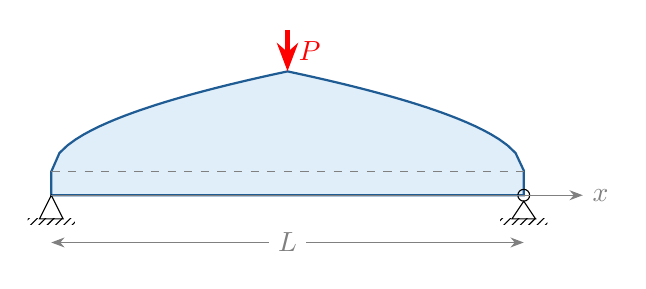
\begin{tikzpicture}[scale=1.5, >=Stealth]
    % Draw equal strength beam (parabolic profile)
    \draw[thick, accent, fill=softblue] (0,-0.2) -- plot[domain=0:2, samples=30] (\x, {0.6*sqrt(\x)}) 
                          -- plot[domain=2:4, samples=30] (\x, {0.6*sqrt(4-\x)}) 
                          -- (4,-0.2) -- cycle;
    
    % Draw axis
    \draw[dashed, gray] (0,0) -- (4,0);
    
    % Supports
    \draw (0,-0.2) -- (-0.1,-0.4) -- (0.1,-0.4) -- cycle;
    \pattern[pattern=north east lines] (-0.2,-0.45) rectangle (0.2,-0.4);
    
    \draw (4,-0.2) circle (0.05);
    \draw (4,-0.25) -- (3.9,-0.4) -- (4.1,-0.4) -- cycle;
    \pattern[pattern=north east lines] (3.8,-0.45) rectangle (4.2,-0.4);
    
    % Load P
    \draw[->, red, ultra thick] (2,1.2) -- node[right] {$P$} (2,0.85);
    
    % Coordinates
    \draw[->, gray] (0,-0.2) -- (4.5,-0.2) node[right] {$x$};
    \draw[<->, gray] (0,-0.6) -- node[fill=white] {$L$} (4,-0.6);
\end{tikzpicture}
\end{center}

\subsubsection*{解答：}

由于简支梁和载荷具有对称性，我们仅需分析左半截面 $x \in [0, L/2]$。

\textbf{1. 确定弯矩方程}
在 $x \in [0, L/2]$ 范围内，梁的支座反力为 $R_A = P/2$，弯矩方程为：
\[
    M(x) = \frac{P}{2} x
\]

\textbf{2. 基于最大正应力条件确定高度 $h(x)$}
对于矩形截面梁（宽为常数 $b$，高度为 $h(x)$），其截面法向抵抗矩为 $W(x) = \frac{1}{6} b h^2(x)$。
截面上的最大正应力必须达到材料的许用应力 $[\sigma]$：
\[
    \sigma_{\max}(x) = \frac{M(x)}{W(x)} = \frac{\frac{P}{2} x}{\frac{1}{6} b h^2(x)} = \frac{3 P x}{b h^2(x)} = [\sigma]
\]
由此求得高度 $h(x)$ 随位置 $x$ 的变化关系为：
\[
    h(x) = \sqrt{\frac{3 P x}{b [\sigma]}}
\]
可见，梁的高度呈抛物线规律变化。在中点 $x = L/2$ 处，高度达到最大值：
\[
    h_{\max} = \sqrt{\frac{3 P L}{2 b [\sigma]}}
\]

\textbf{3. 在铰支座附近应用切应力准则进行校核与修正}
\noindent\textbullet\ 在支座附近 $x \to 0$ 时，弯矩 $M(x) \to 0$，若仅按正应力设计，则 $h(0) \to 0$。然而，支座处的剪力不为零，其值为常数 $V(x) = P/2$。
\noindent\textbullet\ 矩形截面上最大剪应力发生在中性轴处，其计算公式为：
    \[
        \tau_{\max}(x) = \frac{3 V(x)}{2 A(x)} = \frac{3 P}{4 b h(x)}
    \]
\noindent\textbullet\ 按韧性材料的最大切应力准则，许用切应力取 $[\tau]=[\sigma]/2$。因此支座附近要求：
    \[
        \tau_{\max}(x) \le \frac{[\sigma]}{2}
        \implies
        \frac{3 P}{4 b h(x)} \le \frac{[\sigma]}{2}
        \implies
        h(x) \ge h_{\min} = \frac{3 P}{2 b [\sigma]}
    \]
\noindent\textbullet\ 这说明在支座附近，梁的高度必须保持一个常数 $h_{\min}$，以满足抗剪强度要求。

\textbf{4. 确定转换点位置 $x_0$}
当正应力要求的高度等于剪应力要求的最小高度时，对应的轴线位置为 $x_0$：
\[
    \sqrt{\frac{3 P x_0}{b [\sigma]}}
    =
    \frac{3 P}{2 b [\sigma]}
    \implies
    x_0 = \frac{3P}{4b[\sigma]}.
\]

\textbf{结论}：梁的高度 $h(x)$ 与轴线位置 $x$ 的完整关系（左半跨）为：
\[
    h(x) = \begin{cases}
        \dfrac{3 P}{2 b [\sigma]} & x \in \left[ 0, \, \dfrac{3P}{4b[\sigma]} \right] \\[10pt]
        \sqrt{\dfrac{3 P x}{b [\sigma]}} & x \in \left[ \dfrac{3P}{4b[\sigma]}, \, \dfrac{L}{2} \right]
    \end{cases}
\]
右半跨 ($x \in [L/2, L]$) 满足关于跨中对称的分布。


% \newpage removed


\section*{四、受热铝圆柱与钢立柱超静定温度应力分析（20分）}

\textbf{4、在中心铝圆柱 CD 上绕有热电阻丝，通电后将铝圆柱从 $30\text{ °C}$ 加热到 $180\text{ °C}$。在 $30\text{ °C}$ 时，铝圆柱顶端距上面的横梁底面间隙为 $0.7\text{ mm}$。如果设横梁为刚性梁，求两侧钢立柱 AB 和 EF 所受的应力。（铝圆柱截面积为 $375\text{ mm}^2$，钢立柱截面积为 $125\text{ mm}^2$（单侧），铝的弹性模量为 $70\text{ GPa}$，温度膨胀系数为 $23 \times 10^{-6}/\text{°C}$，钢的弹性模量为 $200\text{ GPa}$，钢柱长为 $300\text{ mm}$，铝柱长为 $240\text{ mm}$。）}

\begin{center}
\begin{tikzpicture}[scale=1.2, >=Stealth]
    % Draw rigid top beam
    \draw[ultra thick, fill=gray!30] (-2,2) rectangle (2,2.3);
    \node[above] at (0,2.3) {刚性梁 BF};
    
    % Draw steel columns AB and EF
    \draw[line width=3pt, accent] (-1.5,2) -- (-1.5,-1);
    \draw[line width=3pt, accent] (1.5,2) -- (1.5,-1);
    \node[left] at (-1.5,0.5) {钢柱 AB};
    \node[right] at (1.5,0.5) {钢柱 EF};
    
    % Ground supports for steel columns
    \pattern[pattern=north east lines] (-1.8,-1.2) rectangle (-1.2,-1);
    \draw[thick] (-1.8,-1) -- (-1.2,-1);
    \pattern[pattern=north east lines] (1.2,-1.2) rectangle (1.8,-1);
    \draw[thick] (1.2,-1) -- (1.8,-1);
    
    % Draw aluminum column CD
    \draw[line width=5pt, orange] (0,1.8) -- (0,-1);
    \node[right] at (0,0.4) {铝柱 CD};
    \pattern[pattern=north east lines] (-0.3,-1.2) rectangle (0.3,-1);
    \draw[thick] (-0.3,-1) -- (0.3,-1);
    
    % Gap
    \draw[<->, red, thick] (0,1.8) -- node[fill=white, inner sep=1pt] {$\delta_0$} (0,2.0);
\end{tikzpicture}
\end{center}

\subsubsection*{解答：}

\textbf{1. 自由膨胀变形分析}
若铝圆柱 CD 在不受约束的情况下自由受热膨胀，其温度变形 $\Delta L_{\text{Al}, T}$ 为：
\[
    \Delta L_{\text{Al}, T} = \alpha_{\text{Al}} \cdot \Delta T \cdot L_{\text{Al}}
\]
已知 $\alpha_{\text{Al}} = 23 \times 10^{-6}/\text{°C}$，$\Delta T = 180 - 30 = 150\text{ °C}$，$L_{\text{Al}} = 240\text{ mm}$。代入计算：
\[
    \Delta L_{\text{Al}, T} = 23 \times 10^{-6} \times 150 \times 240 = 0.828\text{ mm}
\]
因为自由膨胀量 $\Delta L_{\text{Al}, T} = 0.828\text{ mm}$ 大于初始间隙 $\delta_0 = 0.7\text{ mm}$，所以铝圆柱的膨胀必定会消除间隙并顶起刚性横梁，使整个系统产生内力（超静定受力状态）。

\textbf{2. 平衡条件分析}
设在平衡状态下，铝圆柱 CD 承受的轴向压紧力为 $F_{\text{Al}}$（以受压为正），两根对称分布的钢立柱承受的轴向拉力均为 $F_{\text{St}}$（以受拉为正）。根据刚性横梁的垂直方向平衡条件：
\[
    \sum F_y = 0 \implies F_{\text{Al}} = 2 F_{\text{St}}
\]

\textbf{3. 变形协调分析}
\noindent\textbullet\ 铝圆柱的实际伸长量为温度膨胀减去受压带来的弹性缩短量：
    \[
        \Delta L_{\text{Al}} = \Delta L_{\text{Al}, T} - \frac{F_{\text{Al}} L_{\text{Al}}}{E_{\text{Al}} A_{\text{Al}}}
    \]
\noindent\textbullet\ 两侧钢立柱的拉伸量为：
    \[
        \Delta L_{\text{St}} = \frac{F_{\text{St}} L_{\text{St}}}{E_{\text{St}} A_{\text{St}}}
    \]
\noindent\textbullet\ 系统整体的变形协调方程为：
    \[
        \Delta L_{\text{Al}} = \delta_0 + \Delta L_{\text{St}}
    \]
    将上式展开：
    \[
        \Delta L_{\text{Al}, T} - \frac{F_{\text{Al}} L_{\text{Al}}}{E_{\text{Al}} A_{\text{Al}}} = \delta_0 + \frac{F_{\text{St}} L_{\text{St}}}{E_{\text{St}} A_{\text{St}}}
    \]

\textbf{4. 联立求解钢立柱的受力}
代入平衡条件 $F_{\text{Al}} = 2 F_{\text{St}}$：
\[
    \Delta L_{\text{Al}, T} - \delta_0 = F_{\text{St}} \left( \frac{2 L_{\text{Al}}}{E_{\text{Al}} A_{\text{Al}}} + \frac{L_{\text{St}}}{E_{\text{St}} A_{\text{St}}} \right)
\]
已知数据为：
\noindent\textbullet\ $\Delta L_{\text{Al}, T} - \delta_0 = 0.828 - 0.7 = 0.128\text{ mm}$
\noindent\textbullet\ 铝的参数：$E_{\text{Al}} = 70\text{ GPa} = 7 \times 10^4\text{ N/mm}^2$，$A_{\text{Al}} = 375\text{ mm}^2$，$L_{\text{Al}} = 240\text{ mm}$
\noindent\textbullet\ 钢的参数：$E_{\text{St}} = 200\text{ GPa} = 2 \times 10^5\text{ N/mm}^2$，$A_{\text{St}} = 125\text{ mm}^2$，$L_{\text{St}} = 300\text{ mm}$

分别计算弹性变形系数：
\[
    \frac{2 L_{\text{Al}}}{E_{\text{Al}} A_{\text{Al}}} = \frac{2 \times 240}{70 \times 10^3 \times 375} = \frac{480}{2.625 \times 10^7} \approx 1.8286 \times 10^{-5}\text{ mm/N}
\]
\[
    \frac{L_{\text{St}}}{E_{\text{St}} A_{\text{St}}} = \frac{300}{200 \times 10^3 \times 125} = \frac{300}{2.5 \times 10^7} = 1.2000 \times 10^{-5}\text{ mm/N}
\]
两项之和为：
\[
    1.8286 \times 10^{-5} + 1.2000 \times 10^{-5} = 3.0286 \times 10^{-5}\text{ mm/N}
\]
从而求得钢立柱承受的拉力 $F_{\text{St}}$：
\[
    F_{\text{St}} = \frac{0.128}{3.0286 \times 10^{-5}} \approx 4226.4\text{ N}
\]

\textbf{5. 计算钢立柱的应力}
钢立柱的轴向拉应力为：
\[
    \sigma_{\text{St}} = \frac{F_{\text{St}}}{A_{\text{St}}} = \frac{4226.4}{125} \approx 33.81\text{ MPa}
\]

\textbf{结论}：加热至 $180\text{ °C}$ 时，两侧钢立柱 AB 和 EF 承受拉应力，其应力大小为：
\[
    \sigma_{\text{St}} = 33.81\text{ MPa}
\]


% \newpage removed


\section*{五、L型悬臂梁弯扭组合变形与危险点分析（20分）}

\textbf{5、L 型悬臂梁自由端受力如图所示，试求距梁固端 $15\text{ cm}$ 处横截面上 D 点和 E 点的应力状态，并用微元法表示。B 端的外力 $F=90\text{ N}$，作用方向与 L 型梁所在平面的垂直方向成 $\theta$ 角度，设 $\theta=45\text{°}$。圆形截面直径 $d = 3\text{ cm}$，直段 AC 总长 $35\text{ cm}$，弯折段 CB 长度为 $7.5\text{ cm}$。}

\begin{center}
\begin{tikzpicture}[scale=1.2, >=Stealth]
    % Draw 3D coordinate system
    \draw[->, gray] (0,0,0) -- (4.5,0,0) node[right] {$x$};
    \draw[->, gray] (0,0,0) -- (0,0,-2.5) node[left] {$y$};
    \draw[->, gray] (0,0,0) -- (0,2.5,0) node[above] {$z$};
    
    % Draw L-beam center line
    \draw[ultra thick, accent] (0,0,0) -- (3,0,0);
    \draw[ultra thick, accent] (3,0,0) -- (3,0,-1.5);
    
    % Nodes
    \node[above left] at (0,0,0) {A (固端)};
    \node[above] at (3,0,0) {C (肘部)};
    \node[right] at (3,0,-1.5) {B (自由端)};
    
    % Target Section
    \draw[fill=softblue, opacity=0.8] (1.2,0,0) circle [radius=3pt];
    \node[above] at (1.2,0.18,0) {D};
    \node[below] at (1.2,-0.18,0) {E};
    \node[below] at (1.2,-0.2,0) {目标截面 ($x=15\text{cm}$)};
    
    % Force F at B
    \draw[dashed] (3,0,-1.5) -- (3,1.5,-1.5);
    \draw[->, red, ultra thick] (3,0,-1.5) -- (3, 1.06, -0.44);
    \node[red, right] at (3, 1.06, -0.44) {$F$};
    \node at (3.3, 0.6, -1.2) {$\theta = 45^\circ$};
\end{tikzpicture}
\end{center}

\subsubsection*{解答：}

\textbf{1. 几何尺寸与截面常数}
\noindent\textbullet\ 从固定端 A ($x = 0$) 到目标截面距离为 $15\text{ cm} = 0.15\text{ m}$，因此目标截面到拐角 C 的长度为：$a = 35 - 15 = 20\text{ cm} = 0.2\text{ m}$。
\noindent\textbullet\ 弯折段 CB 的长度（力臂）为：$b = 7.5\text{ cm} = 0.075\text{ m}$。
\noindent\textbullet\ 圆形截面的几何惯性特征参数为：
\noindent\textbullet\ 面积：$A = \frac{\pi d^2}{4} = \frac{\pi \times 0.03^2}{4} \approx 7.0686 \times 10^{-4}\text{ m}^2$
\noindent\textbullet\ 弯曲截面系数：$W = \frac{\pi d^3}{32} = \frac{\pi \times 0.03^3}{32} \approx 2.6507 \times 10^{-6}\text{ m}^3$
\noindent\textbullet\ 抗扭截面系数：$W_p = \frac{\pi d^3}{16} \approx 5.3014 \times 10^{-6}\text{ m}^3$

\textbf{2. 载荷分解与内力分析}
按原题图，外力位于 L 型梁平面与其法平面构成的斜面内。取
\[
    F_n=F\cos45^\circ=63.64\text{ N},\qquad
    F_p=F\sin45^\circ=63.64\text{ N},
\]
其中 $F_n$ 为垂直于 L 型梁平面的分力，$F_p$ 为 L 型梁平面内的分力。两分力都不是沿直段 AC 的轴力，故目标截面轴力为
\[
    N=0.
\]

目标截面到肘部的距离为 $a=0.20\text{ m}$，短臂为 $b=0.075\text{ m}$。将外力向目标截面形心等效，得到
\[
    T=F_n b=63.64\times0.075=4.773\text{ N}\cdot\text{m},
\]
\[
    M=F_p a=63.64\times0.20=12.728\text{ N}\cdot\text{m}.
\]
由 $F_n a$ 产生的另一弯矩绕另一主轴作用；由于原题图中 D、E 位于上下直径上，对这两个点的正应力贡献为零。

\textbf{3. 计算 D 点和 E 点的应力状态}

按原题图，D 在截面上侧，E 在截面下侧。取拉应力为正，则弯曲正应力为
\[
    \frac{M}{W}
    =\frac{12.728}{2.6507\times10^{-6}}
    =4.80\text{ MPa}.
\]
故
\[
    \sigma_D=+4.80\text{ MPa},\qquad
    \sigma_E=-4.80\text{ MPa}.
\]

扭转剪应力为
\[
    \tau_T=\frac{T}{W_p}
    =\frac{4.773}{5.3014\times10^{-6}}
    =0.900\text{ MPa}.
\]
D、E 位于圆截面外表面。横向剪力引起的截面剪应力在外边界处不作为该边缘微元的主导剪应力叠加；本题 D、E 点剪应力按扭转给出。两点扭转剪应力方向相反，按本文符号约定可写为
\[
    \tau_D=-0.900\text{ MPa},\qquad
    \tau_E=+0.900\text{ MPa}.
\]

\textbf{4. 用微元法表示应力状态}

D点和E点的应力微元（平面应力状态）如下图所示：

\begin{center}
\begin{tikzpicture}[scale=1.5]
    % Element D
    \draw[thick, fill=softblue!30] (0,0) rectangle (1.2,1.2);
    \node at (0.6,0.6) {D};
    
    % Normal stress
    \draw[->, red, thick] (1.2,0.6) -- (1.8,0.6) node[right] {$\sigma_D = 4.80\text{ MPa}$};
    \draw[->, red, thick] (0,0.6) -- (-0.6,0.6);
    
    % Shear stress
    \draw[->, blue, thick] (1.2,1.0) -- (1.2,0.2) node[right] {$\tau_D = -0.90\text{ MPa}$};
    \draw[->, blue, thick] (0,0.2) -- (0,1.0);
    \draw[->, blue, thick] (1.0,1.2) -- (0.2,1.2);
    \draw[->, blue, thick] (0.2,0) -- (1.0,0);
    
    \node[below] at (0.6,-0.3) {(a) D 点微元};
    
    % Element E
    \begin{scope}[xshift=4.5cm]
        \draw[thick, fill=softred!30] (0,0) rectangle (1.2,1.2);
        \node at (0.6,0.6) {E};
        
        % Normal stress (compressive)
        \draw[<-, red, thick] (1.2,0.6) -- (1.8,0.6) node[right] {$\sigma_E = -4.80\text{ MPa}$};
        \draw[<-, red, thick] (0,0.6) -- (-0.6,0.6);
        
        % Shear stress
        \draw[->, blue, thick] (1.2,0.2) -- (1.2,1.0) node[right] {$\tau_E = 0.90\text{ MPa}$};
        \draw[->, blue, thick] (0,1.0) -- (0,0.2);
        \draw[->, blue, thick] (0.2,1.2) -- (1.0,1.2);
        \draw[->, blue, thick] (1.0,0) -- (0.2,0);
        
        \node[below] at (0.6,-0.3) {(b) E 点微元};
    \end{scope}
\end{tikzpicture}
\end{center}


}

\chapter{清华大学 2002 年《工程力学》期末考试题修订解答}
{


\vspace{-1.0cm}

\section*{一、积分求解分布载荷与最大正应力位置题（20分）}

\textbf{1、AB端铰支的工字形截面横梁如图所示，垂直方向受一分布载荷力的作用。所产生的挠度可由如下挠度方程表示：}
\[
    w(x) = \frac{q_0 L^4}{840 EI} \left[ \left(\frac{x}{L}\right)^7 - 7\left(\frac{x}{L}\right)^3 + 6\left(\frac{x}{L}\right) \right]
\]
\textbf{试求：(a) 确定分布载荷的数学表达形式；(b) 确定支撑力 $A_y$，$B_y$ 的表达式；(c) 求梁上最大正应力的位置。}

\subsubsection*{解答：}

以左支座 A 为坐标原点 $x = 0$，向右为 $x$ 轴正方向。设向下为挠度 $w(x)$ 的正方向。

\textbf{(a) 确定分布载荷 $q(x)$ 的数学表达形式}
根据梁的弯曲微分方程，分布载荷 $q(x)$（向下为正）与挠度 $w(x)$ 的关系为：
\[
    q(x) = EI \frac{\diff^4 w(x)}{\diff x^4}
\]
令无量纲参数 $u = \frac{x}{L}$，则有 $w(x) = \frac{q_0 L^4}{840 EI} (u^7 - 7u^3 + 6u)$。对 $x$ 依次求导：
\[
    \frac{\diff w}{\diff x} = \frac{\diff w}{\diff u} \frac{\diff u}{\diff x} = \frac{q_0 L^3}{840 EI} (7u^6 - 21u^2 + 6)
\]
\[
    \frac{\diff^2 w}{\diff x^2} = \frac{q_0 L^2}{840 EI} (42u^5 - 42u) = \frac{q_0 L^2}{20 EI} (u^5 - u)
\]
\[
    \frac{\diff^3 w}{\diff x^3} = \frac{q_0 L}{20 EI} (5u^4 - 1)
\]
\[
    \frac{\diff^4 w}{\diff x^4} = \frac{q_0}{20 EI} (20u^3) = \frac{q_0}{EI} u^3 = \frac{q_0}{EI} \left(\frac{x}{L}\right)^3
\]
代入微分方程中得到：
\[
    q(x) = EI \frac{\diff^4 w(x)}{\diff x^4} = q_0 \left(\frac{x}{L}\right)^3
\]
所以，分布载荷的数学表达形式为 $q(x) = q_0 \left(\frac{x}{L}\right)^3$。

\textbf{(b) 确定支撑力 $A_y$，$B_y$ 的表达式}
根据剪力与挠度三阶导数的关系 $V(x) = -EI \frac{\diff^3 w(x)}{\diff x^3}$，有：
\[
    V(x) = -\frac{q_0 L}{20} \left[ 5\left(\frac{x}{L}\right)^4 - 1 \right]
\]
在简支梁两端，支反力与端部剪力的平衡关系为：
\noindent\textbullet\ 在 A 端 ($x = 0$)：向上支反力 $A_y = V(0) = \frac{q_0 L}{20}$。
\noindent\textbullet\ 在 B 端 ($x = L$)：向上支反力 $B_y = -V(L) = -\left( -\frac{q_0 L}{20} (5 - 1) \right) = \frac{q_0 L}{5}$。

\textit{校核平衡方程：}
1.  垂直方向受力平衡：$\sum F_y = A_y + B_y - \int_0^L q_0 \left(\frac{x}{L}\right)^3 \diff x = \frac{q_0 L}{20} + \frac{q_0 L}{5} - \frac{q_0 L}{4} = 0$。（平衡）
2.  对 A 点力矩平衡：$\sum M_A = B_y \cdot L - \int_0^L x \cdot q_0 \left(\frac{x}{L}\right)^3 \diff x = \frac{q_0 L^2}{5} - \frac{q_0 L^2}{5} = 0$。（平衡）
所以，支撑力表达式为：
\[
    A_y = \frac{q_0 L}{20}, \qquad B_y = \frac{q_0 L}{5}
\]

\textbf{(c) 求梁上最大正应力的位置}
对于等截面直梁，最大弯曲正应力发生在弯矩绝对值 $|M(x)|$ 最大的截面上。弯矩方程为：
\[
    M(x) = EI \frac{\diff^2 w(x)}{\diff x^2} = \frac{q_0 L^2}{20} \left[ \left(\frac{x}{L}\right)^5 - \frac{x}{L} \right]
\]
求弯矩的驻点（令剪力 $V(x) = 0$）：
\[
    \frac{\diff M(x)}{\diff x} = 0 \implies 5\left(\frac{x}{L}\right)^4 - 1 = 0 \implies x = \frac{L}{\sqrt[4]{5}} \approx 0.669 L
\]
因为在 $x=0$ 和 $x=L$ 处弯矩为 0，所以此唯一驻点即为最大弯矩截面。
故梁上最大正应力发生在距 A 端 $x = \frac{L}{\sqrt[4]{5}} \approx 0.669 L$ 处。


% \newpage removed


\section*{二、梁-柱组合结构失稳分析题（20分）}

\textbf{2、简支的横梁上作用了垂直向下的均匀分布载荷 $q$，在中点 C 处有一垂直立柱与之铰接，立柱的 D 点与地面固支。已知横梁和立柱的弹性模量相同，用 $E$ 表示。假设立柱是属于长杆弹性失稳，截面积为 $A$，横梁对 $y$ 轴的惯性矩为 $I_a$，立柱对 $x$ 轴的惯性矩为 $I_b$，对 $y$ 轴的惯性矩为 $I_c$，$I_b/I_c=3/4$。如果结构的破坏为失稳破坏，计算临界载荷集度 $q_{\text{cr}}$。（横梁总长为 $a$，立柱长度为 $L$。）}

\subsubsection*{解答：}

\textbf{1. 梁柱节点 C 的受力与变形协调}

设立柱受到的轴向压力为 $F$。对横梁而言，立柱在 C 点给横梁一个向上的集中力 $F$。
简支梁在均布载荷 $q$ 和中点集中力 $F$ 共同作用下，C 点向下位移为
\[
    w_C = \frac{5 q a^4}{384 E I_a} - \frac{F a^3}{48 E I_a}
\]
立柱轴向压缩量为
\[
    \delta_c=\frac{FL}{EA}.
\]
节点 C 处横梁和立柱铰接，故位移协调条件为
\[
    \frac{5 q a^4}{384 E I_a} - \frac{F a^3}{48 E I_a}
    =
    \frac{FL}{EA}.
\]
由此得到立柱压力与均布载荷集度的关系：
\[
    F
    =
    \frac{5qa}{8}
    \frac{1}{1+\dfrac{48I_aL}{Aa^3}}.
\]

\textbf{2. 立柱临界压力}

立柱底端 D 固定，顶端 C 与横梁铰接。横梁可约束 C 点沿横梁轴向的侧移；
垂直于横梁轴线方向则可按固定-自由柱处理。于是两种可能失稳形式为
\[
    P_{cr,y}
    =
    \frac{\pi^2 E I_c}{(0.7L)^2},
    \qquad
    P_{cr,x}
    =
    \frac{\pi^2 E I_b}{(2L)^2}.
\]
又因 $I_b/I_c=3/4$，有
\[
    P_{cr,x}
    =
    \frac{\pi^2 E I_b}{4L^2},
    \qquad
    P_{cr,y}
    =
    \frac{\pi^2 E I_c}{0.49L^2}
    =
    \frac{4}{3}\frac{\pi^2 E I_b}{0.49L^2}.
\]
显然 $P_{cr,x}<P_{cr,y}$，故立柱绕 $x$ 轴方向失稳控制：
\[
    F_{cr}=P_{cr,x}=\frac{\pi^2 E I_b}{4L^2}.
\]

\textbf{3. 临界载荷集度}

令 $F=F_{cr}$，由上面的 $F-q$ 关系得
\[
    \frac{5q_{cr}a}{8}
    \frac{1}{1+\dfrac{48I_aL}{Aa^3}}
    =
    \frac{\pi^2 E I_b}{4L^2}.
\]
所以
\[
    q_{cr}
    =
    \frac{2\pi^2 E I_b}{5aL^2}
    \left(
    1+\frac{48I_aL}{Aa^3}
    \right).
\]

% \newpage removed


\section*{三、超静定温升极限求解题（20分）}

\textbf{3、在中心铝圆柱 CD 上绕有热电阻丝，通电后将铝圆柱从 $30\text{ °C}$ 开始加热。在 $30\text{ °C}$ 时，铝圆柱顶端距上面的横梁底面间隙为 $0.7\text{ mm}$。如果设横梁为刚性梁，所有材料的安全因数等于 3，求保证系统正常工作时，铝柱能够达到的最高温度。}
\textbf{（铝圆柱截面积为 $375\text{ mm}^2$，钢立柱截面积为 $125\text{ mm}^2$（单侧），铝的弹性模量为 $70\text{ GPa}$，温度膨胀系数为 $23 \times 10^{-6}/\text{°C}$，钢的弹性模量为 $200\text{ GPa}$。铝的屈服极限为 $240\text{ MPa}$，钢的屈服极限为 $220\text{ MPa}$。铝柱长 $L_{\text{Al}} = 240\text{ mm}$，钢柱长 $L_{\text{St}} = 300\text{ mm}$。）}

\subsubsection*{解答：}

\textbf{1. 材料的许用应力计算}
安全因数 $n = 3$，两材料的许用应力（抗拉/抗压强度极限）为：
\noindent\textbullet\ 铝柱：$[\sigma]_{\text{Al}} = \frac{\sigma_{s, \text{Al}}}{n} = \frac{240}{3} = 80\text{ MPa}$
\noindent\textbullet\ 钢柱：$[\sigma]_{\text{St}} = \frac{\sigma_{s, \text{St}}}{n} = \frac{220}{3} = 73.33\text{ MPa}$

\textbf{2. 静力学平衡与强度限制分析}
设铝柱受到的轴向力为 $F_{\text{Al}}$（受压），单侧钢柱受到的轴向力为 $F_{\text{St}}$（受拉）。
平衡关系为：
\[
    F_{\text{Al}} = 2 F_{\text{St}}
\]
根据两材料的许用应力限制系统最大承载力：
\noindent\textbullet\ 若铝柱达到强度极限：$F_{\text{Al}} = [\sigma]_{\text{Al}} A_{\text{Al}} = 80 \times 375 = 30,000\text{ N}$
\noindent\textbullet\ 若钢柱达到强度极限：$F_{\text{St}} = [\sigma]_{\text{St}} A_{\text{St}} = 73.33 \times 125 = 9,166.7\text{ N} \implies F_{\text{Al}} = 2 F_{\text{St}} = 18,333.3\text{ N}$
比较可知，系统强度瓶颈在钢立柱上。因此，系统能承受的最大压紧力限制为：
\[
    F_{\text{Al, max}} = 18,333.3\text{ N}, \qquad F_{\text{St, max}} = 9,166.7\text{ N}
\]

\textbf{3. 变形协调分析与最大温升计算}
根据间隙闭合后的变形协调方程：
\[
    \Delta L_{\text{Al}, T} - \frac{F_{\text{Al}} L_{\text{Al}}}{E_{\text{Al}} A_{\text{Al}}} = \delta_0 + \frac{F_{\text{St}} L_{\text{St}}}{E_{\text{St}} A_{\text{St}}}
\]
将最大限制力代入协调方程，求解此时铝柱所需的自由热膨胀量 $\Delta L_{\text{Al}, T}$：
\[
    \Delta L_{\text{Al}, T} = \delta_0 + F_{\text{St, max}} \left( \frac{2 L_{\text{Al}}}{E_{\text{Al}} A_{\text{Al}}} + \frac{L_{\text{St}}}{E_{\text{St}} A_{\text{St}}} \right)
\]
代入数值计算：
\[
    \frac{2 L_{\text{Al}}}{E_{\text{Al}} A_{\text{Al}}} = \frac{2 \times 240}{70 \times 10^3 \times 375} \approx 1.8286 \times 10^{-5}\text{ mm/N}
\]
\[
    \frac{L_{\text{St}}}{E_{\text{St}} A_{\text{St}}} = \frac{300}{200 \times 10^3 \times 125} = 1.2000 \times 10^{-5}\text{ mm/N}
\]
所以：
\[
    \Delta L_{\text{Al}, T} = 0.7 + 9166.7 \times (1.8286 + 1.2000) \times 10^{-5} = 0.7 + 0.2776 = 0.9776\text{ mm}
\]

由热膨胀公式 $\Delta L_{\text{Al}, T} = \alpha_{\text{Al}} \Delta T L_{\text{Al}}$，求温升 $\Delta T$：
\[
    0.9776 = 23 \times 10^{-6} \times \Delta T \times 240 \implies \Delta T = \frac{0.9776}{5.52 \times 10^{-3}} \approx 177.1\text{ °C}
\]

最高能达到的温度为：
\[
    T_{\max} = T_0 + \Delta T = 30 + 177.1 = 207.1\text{ °C}
\]


% \newpage removed


\section*{四、自行车蹬踏机构轴向弯扭组合应力分析题（20分）}

\textbf{4、自行车的蹬踏系统由下图所示，设人的蹬踏力 $P=750\text{ N}$ 为恒力，在任意时刻都垂直于地面。杆件尺寸为：曲柄臂长 $b_1 = 125\text{ mm}$，脚蹬轴长 $b_2 = 60\text{ mm}$，圆截面轴直径 $d=15\text{ mm}$。当脚蹬子从水平位置 ($\varphi=0$) 运动到最低点位置 ($\varphi=\pi/2$) 过程中：}
\textbf{（a）求连接处 A 点弯矩、扭矩、轴力和剪力的变化；（b）当忽略剪力作用时，求 A 点应力状态的表达形式；（c）用微元法给出 $\varphi=0$，$\varphi=\pi/4$，$\varphi=\pi/2$ 时的应力状态。}

\subsubsection*{解答：}

把 A 截面看作曲柄臂根部截面。取曲柄臂轴线为局部 $s$ 轴，从 A 指向脚蹬；取 $x$ 轴沿脚蹬轴方向，另一个横向主轴记为 $n$。脚蹬从水平位置转到最低位置时，
\[
    0\le \varphi\le \frac{\pi}{2}.
\]
脚蹬中心相对 A 截面的矢径可写成
\[
    \boldsymbol r=b_1\boldsymbol e_s+b_2\boldsymbol e_x,
\]
其中 $b_1=125\text{ mm}$ 为曲柄臂长度，$b_2=60\text{ mm}$ 为脚蹬轴外伸长度。外力始终竖直向下，大小为 $P=750\text{ N}$。

\textbf{(a) A 点内力随转角 $\varphi$ 的变化规律}
将竖直力分解到曲柄臂局部轴线方向和横向方向，可得
\[
    N(\varphi)=P\sin\varphi,\qquad Q(\varphi)=P\cos\varphi.
\]
其中 $N$ 为 A 截面轴力，$Q$ 为横向剪力的合力大小。

A 截面的内力矩由两部分组成：曲柄臂长度 $b_1$ 产生平面弯矩，脚蹬轴外伸 $b_2$ 产生随曲柄角分解的扭矩和侧向弯矩。因此
\[
    M_1(\varphi)=P b_1\cos\varphi,\qquad
    M_2(\varphi)=P b_2\sin\varphi,
\]
\[
    T(\varphi)=P b_2\cos\varphi.
\]
所以 A 截面的合成弯矩为
\[
    M_b(\varphi)=\sqrt{M_1^2+M_2^2}
    =P\sqrt{b_1^2\cos^2\varphi+b_2^2\sin^2\varphi}.
\]
代入 $b_1=0.125\text{ m}$、$b_2=0.060\text{ m}$：
\[
    N=750\sin\varphi,\quad Q=750\cos\varphi,
\]
\[
    M_1=93.75\cos\varphi\,\mathrm{N\cdot m},\quad
    M_2=45\sin\varphi\,\mathrm{N\cdot m},\quad
    T=45\cos\varphi\,\mathrm{N\cdot m}.
\]

\textbf{(b) 忽略剪力作用时 A 点的应力状态}
圆截面面积、抗弯截面系数和抗扭截面系数分别为
\[
    A=\frac{\pi d^2}{4},\qquad W=\frac{\pi d^3}{32},\qquad W_p=\frac{\pi d^3}{16}=2W.
\]
忽略横向剪力时，A 截面危险点的正应力由轴力和弯曲共同产生：
\[
    \sigma_{\max}(\varphi)
    =\frac{N(\varphi)}{A}+\frac{M_b(\varphi)}{W}
    =\frac{4P\sin\varphi}{\pi d^2}
    +\frac{32P}{\pi d^3}
      \sqrt{b_1^2\cos^2\varphi+b_2^2\sin^2\varphi}.
\]
扭转切应力为
\[
    \tau(\varphi)=\frac{T(\varphi)}{W_p}
    =\frac{16P b_2\cos\varphi}{\pi d^3}.
\]
因此危险点处为平面应力状态：
\[
    \sigma=\sigma_{\max}(\varphi),\qquad \tau=\tau(\varphi).
\]
微元作图时，正应力 $\sigma$ 画在轴向外法线面上，拉应力向外、压应力向内；切应力 $\tau$ 按扭矩 $T$ 的右手螺旋方向画在互相垂直的两个面上，并在相邻面上配成平衡剪应力。

\textbf{(c) 典型角度下的应力微元状态表示}
取 $d=0.015\text{ m}$，则 $A=1.767\times10^{-4}\text{ m}^2$，$W=3.313\times10^{-7}\text{ m}^3$，$W_p=6.627\times10^{-7}\text{ m}^3$。
\begin{enumerate}
    \item \textbf{$\varphi=0$：}
    \[
        N=0,\quad Q=P,\quad M_b=P b_1=93.75\,\mathrm{N\cdot m},\quad T=P b_2=45\,\mathrm{N\cdot m}.
    \]
    \[
        \sigma_{\max}=283.0\text{ MPa},\qquad \tau=67.9\text{ MPa}.
    \]
    微元上同时有弯曲正应力和扭转切应力。

    \item \textbf{$\varphi=\pi/4$：}
    \[
        N=\frac{P}{\sqrt2},\quad Q=\frac{P}{\sqrt2},\quad
        M_b=\frac{P}{\sqrt2}\sqrt{b_1^2+b_2^2},\quad
        T=\frac{P b_2}{\sqrt2}.
    \]
    \[
        \sigma_{\max}
        =\frac{4P}{\sqrt2\,\pi d^2}
        +\frac{32P\sqrt{b_1^2+b_2^2}}{\sqrt2\,\pi d^3}
        \approx 225.0\text{ MPa},
    \]
    \[
        \tau=\frac{16P b_2}{\sqrt2\,\pi d^3}\approx48.0\text{ MPa}.
    \]

    \item \textbf{$\varphi=\pi/2$：}
    \[
        N=P,\quad Q=0,\quad M_b=P b_2=45\,\mathrm{N\cdot m},\quad T=0.
    \]
    \[
        \sigma_{\max}
        =\frac{4P}{\pi d^2}+\frac{32P b_2}{\pi d^3}
        \approx 140.1\text{ MPa},\qquad \tau=0.
    \]
\end{enumerate}

三种角度下的危险点微元可按下图誊写，数值单位均为 MPa：
\begin{center}
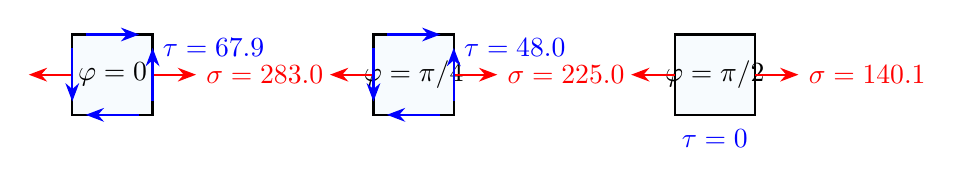
\begin{tikzpicture}[scale=0.85, >=Stealth]
    \draw[thick, fill=softblue!25] (0,0) rectangle (1.2,1.2);
    \node at (0.6,0.6) {$\varphi=0$};
    \draw[->, red, thick] (1.2,0.6) -- (1.85,0.6) node[right] {$\sigma=283.0$};
    \draw[->, red, thick] (0,0.6) -- (-0.65,0.6);
    \draw[->, blue, thick] (1.2,0.2) -- (1.2,1.0) node[right] {$\tau=67.9$};
    \draw[->, blue, thick] (0,1.0) -- (0,0.2);
    \draw[->, blue, thick] (0.2,1.2) -- (1.0,1.2);
    \draw[->, blue, thick] (1.0,0) -- (0.2,0);

    \begin{scope}[xshift=4.5cm]
        \draw[thick, fill=softblue!25] (0,0) rectangle (1.2,1.2);
        \node at (0.6,0.6) {$\varphi=\pi/4$};
        \draw[->, red, thick] (1.2,0.6) -- (1.85,0.6) node[right] {$\sigma=225.0$};
        \draw[->, red, thick] (0,0.6) -- (-0.65,0.6);
        \draw[->, blue, thick] (1.2,0.2) -- (1.2,1.0) node[right] {$\tau=48.0$};
        \draw[->, blue, thick] (0,1.0) -- (0,0.2);
        \draw[->, blue, thick] (0.2,1.2) -- (1.0,1.2);
        \draw[->, blue, thick] (1.0,0) -- (0.2,0);
    \end{scope}

    \begin{scope}[xshift=9.0cm]
        \draw[thick, fill=softblue!25] (0,0) rectangle (1.2,1.2);
        \node at (0.6,0.6) {$\varphi=\pi/2$};
        \draw[->, red, thick] (1.2,0.6) -- (1.85,0.6) node[right] {$\sigma=140.1$};
        \draw[->, red, thick] (0,0.6) -- (-0.65,0.6);
        \node[blue] at (0.6,-0.35) {$\tau=0$};
    \end{scope}
\end{tikzpicture}
\end{center}


% \newpage removed


\section*{五、变宽度变高度等应力悬臂梁设计（20分）}

\textbf{5、有一均布载荷的悬臂梁，任意截面均为矩形，固定端 B 的截面高度为 $h_B$，宽度为 $b_B$。如果梁的宽度随轴线 $x$ 成线性函数变化，即 $b(x) = b_B \frac{x}{L}$（其中 $x$ 自自由端向固定端计量），那么要设计一条等应力梁（即梁任意截面的最大正应力相等），试求梁的高度随 $x$ 变化的关系。}

\subsubsection*{解答：}

\textbf{1. 确定弯矩方程}
设自由端为原点 $x = 0$，固定端为 $x = L$。在距离自由端为 $x$ 的截面上，均布载荷 $q$ 产生的弯矩为：
\[
    M(x) = \frac{1}{2} q x^2
\]

\textbf{2. 确定截面系数 $W(x)$}
截面为矩形，宽度随位置线性变化 $b(x) = b_B \frac{x}{L}$，设截面高度为 $h(x)$。截面抵抗矩为：
\[
    W(x) = \frac{1}{6} b(x) h^2(x) = \frac{b_B x h^2(x)}{6 L}
\]

\textbf{3. 应用等应力条件}
要求任意横截面上的最大弯曲正应力均等于固定端 B 处的最大正应力（即设计为等应力梁）：
\[
    \sigma_{\max}(x) = \frac{M(x)}{W(x)} = \frac{\frac{1}{2} q x^2}{\frac{b_B x h^2(x)}{6 L}} = \frac{3 q L x}{b_B h^2(x)} = \text{常数}
\]
因为在固定端 $x = L$ 处，高度为 $h_B$，其应力为：
\[
    \sigma_{\max}(L) = \frac{3 q L^2}{b_B h_B^2}
\]
令 $\sigma_{\max}(x) = \sigma_{\max}(L)$：
\[
    \frac{3 q L x}{b_B h^2(x)} = \frac{3 q L^2}{b_B h_B^2}
\]
约去两端共同的常数项：
\[
    \frac{x}{h^2(x)} = \frac{L}{h_B^2} \implies h^2(x) = h_B^2 \frac{x}{L} \implies h(x) = h_B \sqrt{\frac{x}{L}}
\]

\textbf{结论}：等应力梁的高度随 $x$ 的变化关系为：
\[
    h(x) = h_B \sqrt{\frac{x}{L}}
\]


}

\chapter{工程力学 2003 年秋季期末考试试题卷 B卷 修订解答}
{
\renewcommand{\assetdir}{../../考题_按知识点整理/visual_assets/question_crops/2003_2003年期末_B卷}


\vspace{-1.0cm}

\section*{一、（25分）}

\textbf{梁 AB 的 A 端固支在左侧的垂直刚性壁面，B 端通过一个滚轴支撑着梁 BC 的左端。梁 BC 的右端为固定铰支约束。设两根梁有相同的弯曲刚度 $EI$ 和相同的长度 $L$，当没有外载荷时，都处于水平状态。当梁 BC 上有垂直向下的均布载荷 $q_0$ 时，求：}
\textbf{(1) BC 梁中点的挠度；}
\textbf{(2) 梁 AB 中点的转角；}
\textbf{(3) 梁 BC 在 C 点的转角；}
\textbf{(4) 两根梁各自截面的最大正应力位置和大小。}

\begin{center}
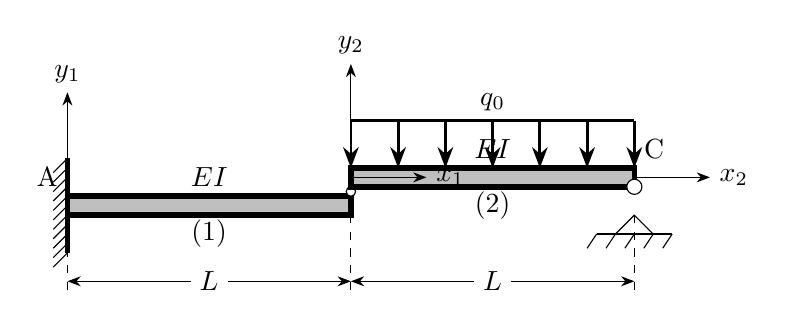
\begin{tikzpicture}[scale=1.2, >=Stealth]
    % Wall A
    \draw [line width=1.5pt] (0, 0.3) -- (0, 1.3);
    \foreach \y in {0.3, 0.4, 0.5, 0.6, 0.7, 0.8, 0.9, 1.0, 1.1, 1.2, 1.3}
        \draw (0,\y) -- (-0.15,\y-0.15);
        
    % Beam AB (1)
    \draw [line width=2.0pt, fill=lightgray] (0, 0.7) rectangle (3.0, 0.9);
    \node at (1.5, 0.5) {(1)};
    \node [above left] at (0, 0.9) {A};
    \node [above right] at (3.0, 0.9) {B};
    \node at (1.5, 1.1) {$EI$};
    
    % Roller support at B
    \draw [fill=white] (3.0, 0.95) circle (0.05);
    
    % Beam BC (2)
    \draw [line width=2.0pt, fill=lightgray] (3.0, 1.0) rectangle (6.0, 1.2);
    \node at (4.5, 0.8) {(2)};
    \node [above right] at (6.0, 1.2) {C};
    \node at (4.5, 1.4) {$EI$};
    
    % Support C (hinge)
    \draw (6.0, 0.7) -- (6.2, 0.5) -- (5.8, 0.5) -- cycle;
    \draw (5.6, 0.5) -- (6.4, 0.5);
    \foreach \x in {5.6, 5.8, 6.0, 6.2, 6.4}
        \draw (\x, 0.5) -- (\x-0.1, 0.35);
    \draw [fill=white] (6.0, 1.0) circle (0.08);
    
    % Distributed load q0 on BC
    \draw [line width=1.0pt, ->] (3.0, 1.7) -- (3.0, 1.2);
    \draw [line width=1.0pt, ->] (3.5, 1.7) -- (3.5, 1.2);
    \draw [line width=1.0pt, ->] (4.0, 1.7) -- (4.0, 1.2);
    \draw [line width=1.0pt, ->] (4.5, 1.7) -- (4.5, 1.2);
    \draw [line width=1.0pt, ->] (5.0, 1.7) -- (5.0, 1.2);
    \draw [line width=1.0pt, ->] (5.5, 1.7) -- (5.5, 1.2);
    \draw [line width=1.0pt, ->] (6.0, 1.7) -- (6.0, 1.2);
    \draw [line width=1.0pt] (3.0, 1.7) -- (6.0, 1.7);
    \node [above] at (4.5, 1.7) {$q_0$};
    
    % Dimensions
    \draw [<->] (0, 0.0) -- (3.0, 0.0) node[midway, fill=white] {$L$};
    \draw [<->] (3.0, 0.0) -- (6.0, 0.0) node[midway, fill=white] {$L$};
    \draw [dashed] (0, 0.7) -- (0, -0.1);
    \draw [dashed] (3.0, 0.7) -- (3.0, -0.1);
    \draw [dashed] (6.0, 0.7) -- (6.0, -0.1);
    
    % Coordinate axis
    \draw [->] (0, 0.8) -- (0, 2.0) node[above] {$y_1$};
    \draw [->] (3.0, 1.1) -- (3.0, 2.3) node[above] {$y_2$};
    \draw [->] (3.0, 1.1) -- (3.8, 1.1) node[right] {$x_1$};
    \draw [->] (6.0, 1.1) -- (6.8, 1.1) node[right] {$x_2$};
\end{tikzpicture}
\end{center}

\subsubsection*{解答：}

根据题目描述，B端滚轴在梁AB和梁BC之间传递垂直反力。设BC梁在左端B点受AB梁向上的支承力为 $R_B$，根据作用力与反作用力关系，AB梁在右端B点承受BC梁施加的垂直向下的集中力，其大小同样为 $R_B$。

\textbf{1. 静定分析与支反力计算} \\
由于BC梁的C端为固定铰支座（弯矩为0），B端仅受滚轴垂直支撑力 $R_B$，且其上作用有向下均布载荷 $q_0$。对BC梁列关于C点的力矩平衡方程：
\[
    \sum M_C = 0 \implies R_B \cdot L - q_0 L \cdot \frac{L}{2} = 0 \implies R_B = \frac{q_0 L}{2}
\]
由此可知，AB梁自由端受到的向下集中力为 $P = R_B = \frac{q_0 L}{2}$。

\textbf{2. 梁 AB 的变形分析} \\
以A端为原点，建立向右为 $x$ 轴、向上为 $y$ 轴的坐标系。梁AB是受自由端集中力 $P = \frac{q_0 L}{2}$ 的悬臂梁。
其弯矩方程为（拉应力在下侧为正）：
\[
    M_{AB}(x) = -P(L - x) = -\frac{q_0 L}{2}(L - x)
\]
根据挠曲线近似微分方程：
\[
    EI w_{AB}''(x) = M_{AB}(x) = -\frac{q_0 L}{2}(L - x)
\]
积分一次，结合固定端边界条件 $w_{AB}'(0) = 0$：
\[
    EI w_{AB}'(x) = -\frac{q_0 L}{2}\left( L x - \frac{1}{2} x^2 \right)
\]
积分两次，结合固定端边界条件 $w_{AB}(0) = 0$：
\[
    EI w_{AB}(x) = -\frac{q_0 L}{2}\left( \frac{1}{2} L x^2 - \frac{1}{6} x^3 \right)
\]
由此可得AB梁自由端B点（$x=L$）的下挠量为：
\[
    w_B = -w_{AB}(L) = \frac{q_0 L}{2EI} \left( \frac{L^3}{2} - \frac{L^3}{6} \right) = \frac{q_0 L^4}{6EI} \quad (\text{向下})
\]
\textbf{(2) 梁 AB 中点的转角}：
将 $x = L/2$ 代入转角方程：
\[
    \theta_{AB}(L/2) = w_{AB}'(L/2) = -\frac{q_0 L}{2EI} \left( L \frac{L}{2} - \frac{L^2}{8} \right) = -\frac{3 q_0 L^3}{16 EI}
\]
绝对值大小为 \textbf{$\frac{3 q_0 L^3}{16 EI}$}，转角方向为\textbf{顺时针}。

\textbf{3. 梁 BC 的变形分析} \\
建立以B端为原点，向右为 $x$ 轴，向上为 $y$ 轴的坐标系。
BC梁的B端处产生向下的位移，其值为AB梁B端的挠度，即 $w_{BC}(0) = -w_B = -\frac{q_0 L^4}{6EI}$。
C端（$x=L$）为铰支座，位移为 $w_{BC}(L) = 0$。
BC梁的弯矩方程为：
\[
    M_{BC}(x) = R_B x - \frac{1}{2}q_0 x^2 = \frac{q_0 L}{2} x - \frac{1}{2}q_0 x^2
\]
近似微分方程为：
\[
    EI w_{BC}''(x) = \frac{q_0 L}{2} x - \frac{1}{2}q_0 x^2
\]
积分一次，引入常数 $C_1$：
\[
    EI w_{BC}'(x) = \frac{q_0 L}{4} x^2 - \frac{q_0}{6} x^3 + C_1
\]
积分两次，引入常数 $C_2$：
\[
    EI w_{BC}(x) = \frac{q_0 L}{12} x^3 - \frac{q_0}{24} x^4 + C_1 x + C_2
\]
代入边界条件：
\begin{itemize}
    \item $x = 0$ 处：$EI w_{BC}(0) = C_2 = -EI w_B = -\frac{q_0 L^4}{6} \implies C_2 = -\frac{q_0 L^4}{6}$
    \item $x = L$ 处：$EI w_{BC}(L) = \frac{q_0 L^4}{12} - \frac{q_0 L^4}{24} + C_1 L - \frac{q_0 L^4}{6} = 0$
          \[
              \frac{q_0 L^4}{24} + C_1 L - \frac{4q_0 L^4}{24} = 0 \implies C_1 L = \frac{3q_0 L^4}{24} = \frac{q_0 L^4}{8} \implies C_1 = \frac{q_0 L^3}{8}
          \]
\end{itemize}
得到BC梁的转角及挠度曲线方程：
\[
    w_{BC}'(x) = \frac{q_0}{24 EI} \left( 6 L x^2 - 4 x^3 + 3 L^3 \right)
\]
\[
    w_{BC}(x) = \frac{q_0}{24 EI} \left( 2 L x^3 - x^4 + 3 L^3 x - 4 L^4 \right)
\]

\textbf{(1) BC 梁中点的挠度}：
将 $x = L/2$ 代入挠度曲线方程：
\[
    w_{BC}(L/2) = \frac{q_0}{24 EI} \left[ 2 L \left(\frac{L^3}{8}\right) - \frac{L^4}{16} + 3 L^3 \left(\frac{L}{2}\right) - 4 L^4 \right] 
    = \frac{q_0 L^4}{24 EI} \left( \frac{1}{4} - \frac{1}{16} + \frac{3}{2} - 4 \right)
\]
\[
    \frac{1}{4} - \frac{1}{16} + \frac{3}{2} - 4 = \frac{4 - 1 + 24 - 64}{16} = -\frac{37}{16}
\]
\[
    w_{BC}(L/2) = -\frac{37 q_0 L^4}{384 EI}
\]
因此，BC梁中点的向下挠度大小为 \textbf{$\frac{37 q_0 L^4}{384 EI}$}。

\textbf{(3) 梁 BC 在 C 点的转角}：
将 $x = L$ 代入转角方程：
\[
    \theta_{BC}(L) = w_{BC}'(L) = \frac{q_0}{24 EI} \left( 6 L^3 - 4 L^3 + 3 L^3 \right) = \frac{5 q_0 L^3}{24 EI}
\]
绝对值大小为 \textbf{$\frac{5 q_0 L^3}{24 EI}$}，转角方向为\textbf{逆时针}。

\textbf{(4) 两根梁各自截面的最大正应力位置和大小}：
设梁的抗弯截面模量为 $W_z$。最大弯曲正应力大小由最大弯矩值确定，计算公式为 $\sigma_{\max} = M_{\max} / W_z$。
\begin{itemize}
    \item \textbf{梁 AB}：
          由于梁AB受自由端集中力作用，最大弯矩发生在固定端A（$x=0$）：
          \[
              |M_{AB}|_{\max} = \frac{q_0 L^2}{2}
          \]
          所以最大拉应力在 \textbf{A端固定截面的上边缘}，大小为 \textbf{$\sigma_{AB,\max} = \frac{q_0 L^2}{2 W_z}$}；同截面下边缘为等值压应力。
    \item \textbf{梁 BC}：
          弯矩方程为 $M_{BC}(x) = \frac{q_0 L}{2} x - \frac{1}{2}q_0 x^2$。
          求导数确定极值位置：$\frac{\diff M_{BC}}{\diff x} = \frac{q_0 L}{2} - q_0 x = 0 \implies x = \frac{L}{2}$。
          最大弯矩发生在BC梁的中点 $x = L/2$ 处：
          \[
              M_{BC,\max} = \frac{q_0 L^2}{4} - \frac{q_0 L^2}{8} = \frac{q_0 L^2}{8}
          \]
          所以最大拉应力在 \textbf{BC梁中点截面的下边缘}，大小为 \textbf{$\sigma_{BC,\max} = \frac{q_0 L^2}{8 W_z}$}；同截面上边缘为等值压应力。
\end{itemize}


% \newpage removed


\section*{二、（25分）}

\textbf{滑雪场缆车由截面为圆环的钢管和车厢构成。钢管的内径 $d_i = 52\text{ mm}$，外径 $d_o = 60\text{ mm}$。与车厢相比，钢管的重量可以忽略不计，车厢的重量为 $W = 2\text{ kN}$。}
\textbf{(a) 确定 C 点的应力分量 $\sigma_{xx}$，$\sigma_{yy}$ 和 $\tau_{xy}$，C 点处于管截面的外表面，并用微元表示。}
\textbf{(b) 计算 C 点的主应力及其方向，计算 C 点的最大切应力。}
\textbf{(c) 计算 DE 段上截面的最大拉伸应力。}

\begin{center}
    \includegraphics[width=0.86\textwidth]{\assetdir/q-002.png}
\end{center}

\subsubsection*{解答：}

\textbf{1. 截面几何性质计算} \\
圆环外径 $d_o = 60\text{ mm}$，内径 $d_i = 52\text{ mm}$。
\begin{itemize}
    \item 截面积
          \[
              A=\frac{\pi}{4}(d_o^2-d_i^2)
              =224\pi\text{ mm}^2
              =703.7\text{ mm}^2 .
          \]
    \item 对形心直径的惯性矩
          \[
              I=\frac{\pi}{64}(d_o^4-d_i^4)
              =2.773\times 10^5\text{ mm}^4 .
          \]
    \item 抗弯截面模量
          \[
              W_z=\frac{I}{d_o/2}
              =9.243\times 10^3\text{ mm}^3 .
          \]
\end{itemize}

\textbf{2. C 截面内力} \\
设局部 $x$ 轴沿斜管轴线，$y$ 轴取题图截面内方向。斜管与水平线成 $45^\circ$，车厢重力 $W=2\text{ kN}$ 在 C 截面上分解为
\begin{itemize}
    \item 轴力
          \[
              N=W\sin45^\circ=1.414\text{ kN}.
          \]
    \item 横向剪力
          \[
              V=W\cos45^\circ=1.414\text{ kN}.
          \]
    \item 对 C 截面的弯矩由题图的 $0.6\text{ m}$ 水平偏距给出：
          \[
              M_z=W(0.6\text{ m})=1.2\text{ kN}\cdot\text{m}.
          \]
\end{itemize}

\textbf{3. C 点应力分析} \\
题图中 C 点在截面前侧外表面，位于弯矩 $M_z$ 对应的中性轴处，因此 $M_z$ 在 C 点不产生弯曲正应力。C 点的正应力只来自轴力；横向剪力在薄壁圆管前侧点可按课程常用近似取 $\tau_{xy}=2V/A$。

\textbf{(a) 应力分量}：
\begin{itemize}
    \item 轴向正应力
          \[
              \sigma_{xx}
              =\frac{N}{A}
              =\frac{1414}{703.7}
              =2.01\text{ MPa}.
          \]
    \item 管外表面无横向面力，故
          \[
              \sigma_{yy}=0 .
          \]
    \item 剪应力
          \[
              \tau_{xy}
              =\frac{2V}{A}
              =\frac{2(1414)}{703.7}
              =4.02\text{ MPa}.
          \]
\end{itemize}
所以 C 点微元为平面应力状态：
\[
    \sigma_{xx}=2.01\text{ MPa},\qquad
    \sigma_{yy}=0,\qquad
    \tau_{xy}=4.02\text{ MPa}.
\]

\begin{center}
\begin{tikzpicture}[scale=1.2, >=Stealth]
    \draw[thick, fill=softblue!25] (0,0) rectangle (1.4,1.4);
    \node at (0.7,0.7) {C};
    \draw[->, red, thick] (1.4,0.7) -- (2.2,0.7) node[right] {$\sigma_{xx}=2.01\text{ MPa}$};
    \draw[->, red, thick] (0,0.7) -- (-0.8,0.7);
    \draw[->, blue, thick] (1.4,0.25) -- (1.4,1.15) node[right] {$\tau_{xy}=4.02\text{ MPa}$};
    \draw[->, blue, thick] (0,1.15) -- (0,0.25);
    \draw[->, blue, thick] (0.25,1.4) -- (1.15,1.4);
    \draw[->, blue, thick] (1.15,0) -- (0.25,0);
    \node[below] at (0.7,-0.35) {$\sigma_{yy}=0$，横向正应力不画};
\end{tikzpicture}
\end{center}

\textbf{(b) 主应力与最大切应力}：
平面主应力为
\[
    \sigma_{1,2}
    =\frac{\sigma_{xx}+\sigma_{yy}}{2}
    \pm
    \sqrt{\left(\frac{\sigma_{xx}-\sigma_{yy}}{2}\right)^2+\tau_{xy}^2}
    =1.005\pm\sqrt{1.005^2+4.02^2}.
\]
故
\[
    \sigma_1=5.15\text{ MPa},\qquad
    \sigma_2=-3.15\text{ MPa}.
\]
主方向满足
\[
    \tan 2\theta_p=\frac{2\tau_{xy}}{\sigma_{xx}-\sigma_{yy}}
    =4.00,\qquad
    \theta_p\approx 38.0^\circ ,
\]
这里的 $\theta_p$ 是从局部 $x$ 轴正向量到 $\sigma_1$ 所在主平面法线的角度，按题图所取正剪应力方向逆时针为正；另一主方向与其相差 $90^\circ$。最大切应力为
\[
    \tau_{\max}
    =
    \sqrt{\left(\frac{\sigma_{xx}-\sigma_{yy}}{2}\right)^2+\tau_{xy}^2}
    =4.15\text{ MPa}.
\]

\textbf{(c) 计算 DE 段上截面的最大拉伸应力} \\
DE段为垂直段。对DE段截面进行内力分析：
\begin{itemize}
    \item 轴向拉力：$F_N^{DE} = W = 2000\text{ N}$（向下悬挂重力引起拉伸）。
    \item 弯矩：整个DE段上均承受恒定弯矩 $M^{DE} = W \cdot e = 2000\text{ N} \times 0.6\text{ m} = 1200\text{ Nm}$。
    \item 剪力为0。
\end{itemize}
DE段的最大拉应力发生在截面拉伸侧的最外侧纤维处：
\[
    \sigma_{\max}^{DE}
    =
    \frac{F_N^{DE}}{A}+\frac{M^{DE}}{W_z}
    =
    \frac{2000}{703.7}
    +
    \frac{1.2\times10^6}{9.243\times10^3}
    =
    2.84\text{ MPa}+129.83\text{ MPa}
    =
    132.67\text{ MPa}.
\]
所以，DE段上的最大拉伸应力为 \textbf{$132.67\text{ MPa}$}。


% \newpage removed


\section*{三、（25分）}

\textbf{简支梁如图(a)，A 端固定铰支，B 端滚轴铰支，梁上作用有垂直向下的函数分布载荷，若梁的挠度以向上为正，其表达式为：}
\[
    w = \frac{q_0 L^4}{\pi^4 EI} \left[ -16 \cos\left(\frac{\pi x}{2L}\right) + \frac{2\pi^2}{3}\left(\frac{x}{L}\right)^3 - 2\pi^2\left(\frac{x}{L}\right)^2 + \left(\frac{4\pi^2}{3} - 16\right)\left(\frac{x}{L}\right) + 16 \right]
\]
\textbf{(1) 求梁上分布载荷函数的表达式；}
\textbf{(2) 求 A 和 B 点的约束力；}
\textbf{(3) 求梁上最大正应力的位置和大小；}
\textbf{(4) 如果在 AB 梁的中点 C 处增加一个滚轴约束(如图 (b))，求此滚轴的约束力。}

\begin{center}
\begin{tikzpicture}[scale=1.2, >=Stealth]
    % Beam (a)
    \draw [line width=2.5pt, fill=lightgray] (0, 1.8) rectangle (5.0, 2.0);
    \node [above left] at (0, 2.0) {A};
    \node [above right] at (5.0, 2.0) {B};
    \node at (2.5, 1.5) {$EI = \text{const}$};
    \node at (5.3, 1.9) {(a)};
    
    % Hinge A
    \draw (0, 1.5) -- (0.2, 1.3) -- (-0.2, 1.3) -- cycle;
    \draw (-0.3, 1.3) -- (0.3, 1.3);
    \foreach \x in {-0.3, -0.1, 0.1, 0.3}
        \draw (\x, 1.3) -- (\x-0.1, 1.15);
        
    % Roller B
    \draw (5.0, 1.5) -- (5.2, 1.3) -- (4.8, 1.3) -- cycle;
    \draw (4.6, 1.3) -- (5.4, 1.3);
    \draw [fill=white] (4.9, 1.2) circle (0.05);
    \draw [fill=white] (5.1, 1.2) circle (0.05);
    \draw (4.6, 1.1) -- (5.4, 1.1);
    \foreach \x in {4.6, 4.8, 5.0, 5.2, 5.4}
        \draw (\x, 1.1) -- (\x-0.1, 0.95);
        
    % Distributed Load q(x) (a)
    \draw [domain=0:5, samples=100, smooth, variable=\x, line width=1.0pt] plot ({\x}, {2.0 + 0.8*cos(\x*18.0)});
    \foreach \x in {0, 0.5, 1.0, 1.5, 2.0, 2.5, 3.0, 3.5, 4.0, 4.5, 5.0}
        \draw [->, line width=0.8pt] (\x, {2.0 + 0.8*cos(\x*18.0)}) -- (\x, 2.0);
    \node [left] at (0, 2.8) {$q_0$};
    \node [above] at (2.5, 2.6) {函数分布载荷};
    
    % Beam (b)
    \begin{scope}[yshift=-2.0cm]
        \draw [line width=2.5pt, fill=lightgray] (0, 1.8) rectangle (5.0, 2.0);
        \node [above left] at (0, 2.0) {A};
        \node [above right] at (5.0, 2.0) {B};
        \node [below] at (2.5, 1.8) {C};
        \node at (5.3, 1.9) {(b)};
        
        % Hinge A
        \draw (0, 1.5) -- (0.2, 1.3) -- (-0.2, 1.3) -- cycle;
        \draw (-0.3, 1.3) -- (0.3, 1.3);
        \foreach \x in {-0.3, -0.1, 0.1, 0.3}
            \draw (\x, 1.3) -- (\x-0.1, 1.15);
            
        % Roller B
        \draw (5.0, 1.5) -- (5.2, 1.3) -- (4.8, 1.3) -- cycle;
        \draw (4.6, 1.3) -- (5.4, 1.3);
        \draw [fill=white] (4.9, 1.2) circle (0.05);
        \draw [fill=white] (5.1, 1.2) circle (0.05);
        \draw (4.6, 1.1) -- (5.4, 1.1);
        \foreach \x in {4.6, 4.8, 5.0, 5.2, 5.4}
            \draw (\x, 1.1) -- (\x-0.1, 0.95);
            
        % Roller C
        \draw (2.5, 1.5) -- (2.7, 1.3) -- (2.3, 1.3) -- cycle;
        \draw (2.1, 1.3) -- (2.9, 1.3);
        \draw [fill=white] (2.4, 1.2) circle (0.05);
        \draw [fill=white] (2.6, 1.2) circle (0.05);
        \draw (2.1, 1.1) -- (2.9, 1.1);
        \foreach \x in {2.1, 2.3, 2.5, 2.7, 2.9}
            \draw (\x, 1.1) -- (\x-0.1, 0.95);
            
        % Distributed Load q(x) (b)
        \draw [domain=0:5, samples=100, smooth, variable=\x, line width=1.0pt] plot ({\x}, {2.0 + 0.8*cos(\x*18.0)});
        \foreach \x in {0, 0.5, 1.0, 1.5, 2.0, 2.5, 3.0, 3.5, 4.0, 4.5, 5.0}
            \draw [->, line width=0.8pt] (\x, {2.0 + 0.8*cos(\x*18.0)}) -- (\x, 2.0);
    \end{scope}
    
    % Dimensions
    \draw [<->] (0, -0.6) -- (5.0, -0.6) node[midway, fill=white] {$L$};
    \draw [dashed] (0, 1.8) -- (0, -0.7);
    \draw [dashed] (5.0, 1.8) -- (5.0, -0.7);
    \draw [dashed, ->] (0, 2.0) -- (0, 3.2) node[above] {$y,w$};
    \draw [dashed, ->] (0, 2.0) -- (5.8, 2.0) node[right] {$x$};
\end{tikzpicture}
\end{center}

\subsubsection*{解答：}

\textbf{(1) 求梁上分布载荷函数的表达式} \\
已知梁的挠度 $w(x)$ 向上为正。根据梁的弯曲基本微分方程：
\[
    EI \frac{\diff^4 w}{\diff x^4} = -q(x) \implies q(x) = -EI \frac{\diff^4 w}{\diff x^4}
\]
（其中负号表示分布载荷 $q(x)$ 的方向向下）。我们将 $w(x)$ 对 $x$ 依次求四次导数：
\[
    w(x) = \frac{q_0 L^4}{\pi^4 EI} \left[ -16 \cos\left(\frac{\pi x}{2L}\right) + \frac{2\pi^2}{3}\left(\frac{x}{L}\right)^3 - 2\pi^2\left(\frac{x}{L}\right)^2 + \left(\frac{4\pi^2}{3} - 16\right)\left(\frac{x}{L}\right) + 16 \right]
\]
设 $w(x) = \frac{q_0 L^4}{\pi^4 EI} f(x)$，则有：
\begin{align*}
    f'(x) &= 16 \left(\frac{\pi}{2L}\right) \sin\left(\frac{\pi x}{2L}\right) + \frac{2\pi^2}{L^3} x^2 - \frac{4\pi^2}{L^2} x + \frac{1}{L}\left(\frac{4\pi^2}{3} - 16\right) \\
    f''(x) &= 16 \left(\frac{\pi}{2L}\right)^2 \cos\left(\frac{\pi x}{2L}\right) + \frac{4\pi^2}{L^3} x - \frac{4\pi^2}{L^2} = \frac{4\pi^2}{L^2}\left[ \cos\left(\frac{\pi x}{2L}\right) + \frac{x}{L} - 1 \right] \\
    f'''(x) &= -\frac{2\pi^3}{L^3} \sin\left(\frac{\pi x}{2L}\right) + \frac{4\pi^2}{L^3} \\
    f^{(4)}(x) &= -\frac{\pi^4}{L^4} \cos\left(\frac{\pi x}{2L}\right)
\end{align*}
代入四阶微分关系：
\[
    q(x) = -EI \frac{q_0 L^4}{\pi^4 EI} f^{(4)}(x) = -\frac{q_0 L^4}{\pi^4} \left[ -\frac{\pi^4}{L^4} \cos\left(\frac{\pi x}{2L}\right) \right] = q_0 \cos\left(\frac{\pi x}{2L}\right)
\]
所以，梁上向下作用的分布载荷函数表达式为：\textbf{$q(x) = q_0 \cos\left(\frac{\pi x}{2L}\right)$}。

\textbf{(2) 求 A 和 B 点的约束力} \\
A、B两点的垂直支座反力设为向上为正，分别记作 $R_A$ 和 $R_B$。
采用同一内力约定 $V(x)=EIw'''(x)$。端部支反力与梁内剪力方向相反，故左端 $R_A=V(0^+)$，右端 $R_B=-V(L^-)$：
\begin{itemize}
    \item \textbf{A端支反力}（$x = 0$ 处）：
          \[
              R_A = V(0^+) = EI w'''(0) = EI \frac{q_0 L^4}{\pi^4 EI} f'''(0) 
              = \frac{q_0 L^4}{\pi^4} \left( \frac{4\pi^2}{L^3} \right) = \frac{4 q_0 L}{\pi^2}
          \]
    \item \textbf{B端支反力}（$x = L$ 处）：
          \[
              R_B = -V(L^-) = -EI w'''(L) = -EI \frac{q_0 L^4}{\pi^4 EI} f'''(L)
              = -\frac{q_0 L^4}{\pi^4} \left[ -\frac{2\pi^3}{L^3} \sin\left(\frac{\pi}{2}\right) + \frac{4\pi^2}{L^3} \right] 
          \]
          \[
              R_B = -\frac{q_0 L^4}{\pi^4} \left( -\frac{2\pi^3}{L^3} + \frac{4\pi^2}{L^3} \right) = q_0 L \left( \frac{2}{\pi} - \frac{4}{\pi^2} \right)
          \]
\end{itemize}
（静力平衡校验：总外载荷 $F_{\text{total}} = \int_0^L q_0 \cos(\frac{\pi x}{2L}) \diff x = \frac{2q_0 L}{\pi}$，而 $R_A + R_B = \frac{4q_0 L}{\pi^2} + \frac{2q_0 L}{\pi} - \frac{4q_0 L}{\pi^2} = \frac{2q_0 L}{\pi}$，校验无误）。
所以支反力为：\textbf{$R_A = \frac{4 q_0 L}{\pi^2}$}， \textbf{$R_B = q_0 L \left( \frac{2}{\pi} - \frac{4}{\pi^2} \right)$}。

\textbf{(3) 求梁上最大正应力的位置和大小} \\
截面上的正应力由弯矩决定。简支梁的弯矩方程为 $M(x) = EI w''(x)$：
\[
    M(x) = EI \frac{q_0 L^4}{\pi^4 EI} f''(x) = \frac{4 q_0 L^2}{\pi^2} \left[ \cos\left(\frac{\pi x}{2L}\right) + \frac{x}{L} - 1 \right]
\]
寻找弯矩取得极值的截面位置，令其关于 $x$ 的一阶导数（即剪力）等于0：
\[
    \frac{\diff M(x)}{\diff x} = \frac{4 q_0 L}{\pi^2} \left[ -\frac{\pi}{2L} \sin\left(\frac{\pi x}{2L}\right) + \frac{1}{L} \right] = 0 \implies \sin\left(\frac{\pi x}{2L}\right) = \frac{2}{\pi}
\]
由此解得极值点坐标 $x_m$ 满足：
\[
    \frac{\pi x_m}{2L} = \arcsin\left(\frac{2}{\pi}\right) \approx 0.6901\text{ rad} \implies x_m \approx 0.4393 L
\]
该截面处的最大弯矩大小为：
\[
    M_{\max} = |M(x_m)| = \frac{4 q_0 L^2}{\pi^2} \left[ \sqrt{1 - \left(\frac{2}{\pi}\right)^2} + \frac{2}{\pi} \arcsin\left(\frac{2}{\pi}\right) - 1 \right]
\]
代入数值计算：
\[
    M_{\max} \approx \frac{4 q_0 L^2}{\pi^2} \left( 0.7712 + 0.4393 - 1 \right) \approx 0.0853 q_0 L^2
\]
最大弯曲正应力位于 \textbf{$x \approx 0.4393 L$} 截面，大小为 \textbf{$\sigma_{\max} = \frac{0.0853 q_0 L^2}{W_z}$}。

\textbf{(4) 如果在 AB 梁的中点 C 处增加一个滚轴约束，求此滚轴的约束力} \\
这是一个一次超静定结构。选用力法求解，以C端去掉滚轴后的静定简支梁为基本体系，C端向上反力 $R_C$ 为多余未知力。
变形协调条件为：中点 C 处的实际挠度为 0：
\[
    w_C = w_C^{(0)} + w_C^{(R)} = 0
\]
\begin{itemize}
    \item $w_C^{(0)}$：基本体系在中点 C ($x = L/2$) 处由荷载 $q(x)$ 引起的向上挠度：
          \[
              w_C^{(0)} = w(L/2) = \frac{q_0 L^4}{\pi^4 EI} \left[ -16 \cos\left(\frac{\pi}{4}\right) + \frac{2\pi^2}{3}\left(\frac{1}{8}\right) - 2\pi^2\left(\frac{1}{4}\right) + \left(\frac{4\pi^2}{3} - 16\right)\frac{1}{2} + 16 \right]
          \]
          \[
              w_C^{(0)} = \frac{q_0 L^4}{\pi^4 EI} \left( -8\sqrt{2} + \frac{\pi^2}{12} - \frac{\pi^2}{2} + \frac{2\pi^2}{3} + 8 \right) = \frac{q_0 L^4}{\pi^4 EI} \left( 8 - 8\sqrt{2} + \frac{\pi^2}{4} \right)
          \]
    \item $w_C^{(R)}$：多余反力 $R_C$（向上）在中点 C 处引起的向上挠度：
          \[
              w_C^{(R)} = \frac{R_C L^3}{48 EI}
          \]
\end{itemize}
由变形协调方程：
\[
    \frac{q_0 L^4}{\pi^4 EI} \left( 8 - 8\sqrt{2} + \frac{\pi^2}{4} \right) + \frac{R_C L^3}{48 EI} = 0
\]
解出滚轴反力 $R_C$：
\[
    R_C = \frac{48 q_0 L}{\pi^4} \left( 8\sqrt{2} - 8 - \frac{\pi^2}{4} \right) \approx 0.417 q_0 L \quad (\text{方向向上})
\]


% \newpage removed


\section*{五、（25分）}

\textbf{一端固支，另一端自由的横梁上作用了垂直向下的线性分布载荷，A 端的载荷集度为 $q/2$，B 端的载荷集度为 $q$。在中点 C 处有一垂直立柱与横梁用一个球铰连接，立柱的 D 点与地面固支。已知横梁和立柱的弹性模量分别为 $E_{AB}$ 和 $E_{CD}$。假设立柱是属于长杆弹性失稳，截面积为 $A$，横梁对 $z$ 轴的惯性矩为 $I_a$，立柱对 $x$ 轴的惯性矩为 $I_b$，对 $z$ 轴的惯性矩为 $I_c$，$I_b < I_c$。如果结构的破坏为失稳破坏，计算 B 端临界载荷集度 $q_{\text{cr}}$。}

\begin{center}
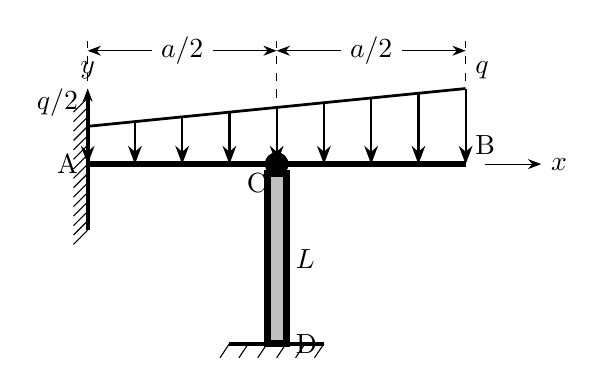
\begin{tikzpicture}[scale=1.2, >=Stealth]
    % Wall A
    \draw [line width=1.5pt] (0, 1.3) -- (0, 2.7);
    \foreach \y in {1.3, 1.4, 1.5, 1.6, 1.7, 1.8, 1.9, 2.0, 2.1, 2.2, 2.3, 2.4, 2.5, 2.6, 2.7}
        \draw (0,\y) -- (-0.15,\y-0.15);
        
    % Beam AB
    \draw [line width=2.0pt] (0, 2.0) -- (4.0, 2.0);
    \node [left] at (0, 2.0) {A};
    \node [above right] at (4.0, 2.0) {B};
    \node [below left] at (2.0, 2.0) {C};
    
    % Column CD
    \draw [line width=2.5pt, fill=lightgray] (1.9, 0.1) rectangle (2.1, 1.9);
    \node [right] at (2.1, 1.0) {$L$};
    \node [right] at (2.1, 0.1) {D};
    
    % Ball Joint C
    \draw [fill=black] (2.0, 2.0) circle (0.12);
    
    % Support D
    \draw [line width=1.5pt] (1.5, 0.1) -- (2.5, 0.1);
    \foreach \x in {1.5, 1.7, 1.9, 2.1, 2.3, 2.5}
        \draw (\x, 0.1) -- (\x-0.1, -0.05);
        
    % Distributed Load q(x)
    \draw [domain=0:4, samples=100, smooth, variable=\x, line width=1.0pt] plot ({\x}, {2.0 + 0.4 + 0.1*\x});
    \foreach \x in {0, 0.5, 1.0, 1.5, 2.0, 2.5, 3.0, 3.5, 4.0}
        \draw [->, line width=0.8pt] (\x, {2.4 + 0.1*\x}) -- (\x, 2.0);
    \node [above left] at (0, 2.4) {$q/2$};
    \node [above right] at (4.0, 2.8) {$q$};
    
    % Dimensions
    \draw [<->] (0, 3.2) -- (2.0, 3.2) node[midway, fill=white] {$a/2$};
    \draw [<->] (2.0, 3.2) -- (4.0, 3.2) node[midway, fill=white] {$a/2$};
    \draw [dashed] (0, 2.0) -- (0, 3.3);
    \draw [dashed] (2.0, 2.0) -- (2.0, 3.3);
    \draw [dashed] (4.0, 2.0) -- (4.0, 3.3);
    
    % Coordinates
    \draw [->] (4.2, 2.0) -- (4.8, 2.0) node[right] {$x$};
    \draw [->] (0, 2.2) -- (0, 2.8) node[above] {$y$};
\end{tikzpicture}
\end{center}

\subsubsection*{解答：}

这是一个涉及压杆稳定与梁的组合受力超静定问题。

\textbf{1. 压杆的临界载荷 $P_{\text{cr}}$ 分析} \\
立柱 CD 的下端 D 为固定端，上端 C 采用球铰与横梁相连。
题目只说明 C 端为球铰连接、D 端固支，没有给出防止立柱侧向位移的额外支撑。因此按最不利的弱轴失稳计算：立柱绕 $x$ 轴弯曲，惯性矩取 $I_b$；边界条件为下端固支、上端可侧移转动，取有效长度系数 $\mu=2.0$。由于 $I_b<I_c$，该方向控制失稳：
\[
    P_{\text{cr}}
    =\frac{\pi^2 E_{CD}I_b}{(2L)^2}
    =\frac{\pi^2 E_{CD}I_b}{4L^2}.
\]

\textbf{2. 线性分布载荷下梁的变形分析} \\
横梁 AB 上的线性分布载荷为 $q(x) = \frac{q}{2} + \frac{q}{2a} x$（以A为原点 $x \in [0, a]$）。
设立柱对横梁 C 点产生的垂直向上推力为 $R_C$。
根据叠加法，C 点的净下挠度由分布载荷 $q(x)$ 引起的下挠度 $w_C^{(q)}$ 和反力 $R_C$ 引起的上挠度 $w_C^{(R)}$ 组合而成。
\begin{enumerate}
    \item \textbf{分布载荷 $q(x)$ 引起的 C 点下挠度 $w_C^{(q)}$}：
          将分布载荷分解为均布载荷 $q_1 = q/2$ 和三角形分布载荷 $q_2(x) = \frac{q}{2a} x$：
          \begin{itemize}
              \item 均布载荷 $q_1 = q/2$ 引起的中点下挠度：
                    \[
                        w_{C1} = \frac{(q/2) (a/2)^2}{24 E_{AB} I_a} \left[ 6a^2 - 4a(a/2) + (a/2)^2 \right] = \frac{17 q a^4}{768 E_{AB} I_a}
                    \]
              \item 三角形载荷 $q_2(x) = \frac{q}{2a} x$ 引起的弯矩为 $M_2(x) = -\frac{q}{12a} (2a^3 - 3a^2 x + x^3)$。
                    根据微分方程积分，求得中点处的下挠度为：
                    \[
                        w_{C2} = \frac{121 q a^4}{7680 E_{AB} I_a}
                    \]
              \item 叠加得到总下挠度：
                    \[
                        w_C^{(q)} = w_{C1} + w_{C2} = \frac{170 q a^4 + 121 q a^4}{7680 E_{AB} I_a} = \frac{291 q a^4}{7680 E_{AB} I_a} = \frac{97 q a^4}{2560 E_{AB} I_a}
                    \]
          \end{itemize}
    \item \textbf{集中反力 $R_C$ 引起的 C 点向上挠度 $w_C^{(R)}$}：
          \[
              w_C^{(R)} = \frac{R_C (a/2)^3}{3 E_{AB} I_a} = \frac{R_C a^3}{24 E_{AB} I_a}
          \]
\end{enumerate}

\textbf{3. 变形协调条件与临界状态} \\
C 点的实际下挠度等于立柱的轴向压缩量 $\Delta L = \frac{R_C L}{E_{CD} A}$：
\[
    w_C^{(q)} - w_C^{(R)} = \frac{R_C L}{E_{CD} A} \implies \frac{97 q a^4}{2560 E_{AB} I_a} - \frac{R_C a^3}{24 E_{AB} I_a} = \frac{R_C L}{E_{CD} A}
\]
解得立柱承受的压力 $R_C$ 与荷载集度 $q$ 的关系为：
\[
    R_C = \frac{\frac{97 q a^4}{2560 E_{AB} I_a}}{\frac{a^3}{24 E_{AB} I_a} + \frac{L}{E_{CD} A}}
\]
在临界破坏状态，立柱承受的压力达到临界屈曲力，即 $R_C = P_{\text{cr}}$。
代入关系式，求得临界载荷集度 $q_{\text{cr}}$：
\[
    q_{\text{cr}} = \frac{2560 E_{AB} I_a}{97 a^4} \left( \frac{a^3}{24 E_{AB} I_a} + \frac{L}{E_{CD} A} \right) P_{\text{cr}}
\]
代入控制临界力，得到本题的临界载荷集度
\[
    q_{\text{cr}}
    =
    \frac{2560 E_{AB} I_a}{97a^4}
    \left(
        \frac{a^3}{24E_{AB}I_a}
        +\frac{L}{E_{CD}A}
    \right)
    \frac{\pi^2E_{CD}I_b}{4L^2}.
\]

}

\chapter{2004 工程力学期中考试解答}
{
\renewcommand{\assetdir}{../../考题_按知识点整理/visual_assets/question_crops/2004_2004工程力学期中考试}



\section*{一、三角形分布载荷梁的剪力和弯矩}

\textbf{一、（30分）\\
两端简支梁AD长，AB端上为线性分布载荷，A端最小载荷集度为零，B端最大载荷集度为$q_0$，在C处作用一个集中载荷$P$，$q_0 = P/L$，试求：\\
a) A端和D端的约束力；\\
b) 写出梁的剪力和弯矩方程；\\
c) 画出剪力和弯矩图。}

\begin{center}
    \includegraphics[width=0.92\linewidth]{\assetdir/q-001.png}
\end{center}

取 A 点为坐标原点，向右为 $x$ 正方向。题图中
\[
    A:0,\qquad B:L,\qquad C:\frac{4L}{3},\qquad D:\frac{5L}{3}.
\]
AB 段线性分布载荷为
\[
    q(x)=q_0\frac{x}{L}=\frac{P}{L^2}x,\qquad 0\le x\le L.
\]
该三角形载荷的合力为
\[
    W=\frac12 q_0L=\frac{P}{2},
\]
作用点距 A 为 $2L/3$。由整体平衡：
\[
    R_A+R_D=\frac{P}{2}+P=\frac{3P}{2},
\]
\[
    R_D\frac{5L}{3}
    =\frac{P}{2}\frac{2L}{3}+P\frac{4L}{3}
    =\frac{5PL}{3}.
\]
故
\[
    R_D=P,\qquad R_A=\frac{P}{2}.
\]

梁的剪力方程为
\[
F_Q(x)=
\begin{cases}
\dfrac{P}{2}-\dfrac{P x^2}{2L^2},&0\le x\le L,\\[6pt]
0,&L\le x\le \dfrac{4L}{3},\\[6pt]
-P,&\dfrac{4L}{3}\le x\le \dfrac{5L}{3}.
\end{cases}
\]
梁的弯矩方程为
\[
M(x)=
\begin{cases}
\dfrac{P}{2}x-\dfrac{P}{6L^2}x^3,&0\le x\le L,\\[6pt]
\dfrac{PL}{3},&L\le x\le \dfrac{4L}{3},\\[6pt]
P\left(\dfrac{5L}{3}-x\right),&
\dfrac{4L}{3}\le x\le \dfrac{5L}{3}.
\end{cases}
\]
其中
\[
    M(0)=0,\qquad M(L)=M\left(\frac{4L}{3}\right)=\frac{PL}{3},\qquad M\left(\frac{5L}{3}\right)=0.
\]

\begin{figure}[H]
\centering
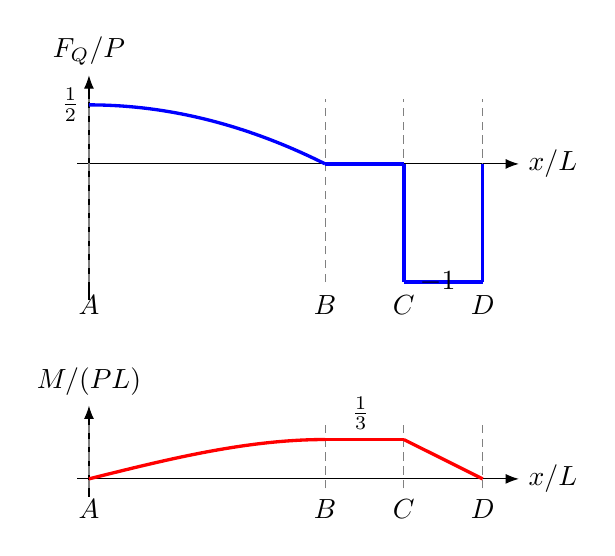
\begin{tikzpicture}[x=3.0cm,y=1.5cm,>=Latex]
  \draw[->] (-0.05,0) -- (1.82,0) node[right] {$x/L$};
  \draw[->] (0,-1.15) -- (0,0.75) node[above] {$F_Q/P$};
  \foreach \x/\lab in {0/A,1/B,1.333/C,1.667/D}{
    \draw[densely dashed,gray] (\x,-1.0)--(\x,0.55);
    \node[below] at (\x,-1.03) {$\lab$};
  }
  \draw[very thick,blue,domain=0:1,samples=80] plot (\x,{0.5-0.5*\x*\x});
  \draw[very thick,blue] (1,0)--(1.333,0);
  \draw[very thick,blue] (1.333,0)--(1.333,-1);
  \draw[very thick,blue] (1.333,-1)--(1.667,-1);
  \draw[very thick,blue] (1.667,-1)--(1.667,0);
  \node[left] at (0,0.5) {$\frac12$};
  \node[right] at (1.36,-1) {$-1$};

  \begin{scope}[yshift=-4.0cm]
    \draw[->] (-0.05,0) -- (1.82,0) node[right] {$x/L$};
    \draw[->] (0,-0.15) -- (0,0.62) node[above] {$M/(PL)$};
    \foreach \x/\lab in {0/A,1/B,1.333/C,1.667/D}{
      \draw[densely dashed,gray] (\x,-0.08)--(\x,0.50);
      \node[below] at (\x,-0.09) {$\lab$};
    }
    \draw[very thick,red,domain=0:1,samples=80] plot (\x,{0.5*\x-\x*\x*\x/6});
    \draw[very thick,red] (1,0.333)--(1.333,0.333);
    \draw[very thick,red] (1.333,0.333)--(1.667,0);
    \node[above] at (1.15,0.333) {$\frac13$};
  \end{scope}
\end{tikzpicture}
\caption{题 1 剪力图和弯矩图}
\end{figure}


% \newpage removed


\section*{二、均布载荷悬臂等应力梁的高度变化}

\textbf{二、（30分）\\
有一均布载荷的悬臂梁，任意截面均为矩形，固定端B的截面高度为$h_B$，宽度为$b_B$。如果梁的宽度随轴线x成线性函数变化，即$b_x=b_Bx/L$，那么要设计一条等应力梁（即梁任意截面上的最大正应力相等），试求梁的高度随x变化的关系。}

\begin{center}
    \includegraphics[width=0.92\linewidth]{\assetdir/q-002.png}
\end{center}

取自由端 A 为 $x=0$，固定端 B 为 $x=L$。从自由端到任意截面 $x$，均布载荷在该截面产生的弯矩为
\[
    M(x)=\frac{q x^2}{2}.
\]
矩形截面宽度已给定为
\[
    b_x=b_B\frac{x}{L}.
\]
矩形截面对弯曲的截面系数为
\[
    W_x=\frac{b_x h_x^2}{6}
    =\frac{b_B x}{L}\frac{h_x^2}{6}.
\]
最大弯曲正应力为
\[
    \sigma_{\max}(x)
    =\frac{M(x)}{W_x}
    =\frac{q x^2/2}{b_B x h_x^2/(6L)}
    =\frac{3qLx}{b_Bh_x^2}.
\]
等应力要求 $\sigma_{\max}(x)$ 与固定端处应力相等。固定端截面应力为
\[
    \sigma_{\max}(L)=\frac{3qL^2}{b_Bh_B^2}.
\]
于是
\[
    \frac{3qLx}{b_Bh_x^2}
    =\frac{3qL^2}{b_Bh_B^2}
    \quad\Longrightarrow\quad
    h_x^2=h_B^2\frac{x}{L}.
\]
因此梁高随 $x$ 的变化关系为
\[
    h_x=h_B\sqrt{\frac{x}{L}},\qquad 0\le x\le L.
\]


% \newpage removed


\section*{三、L 型圆管 B 截面内力与应力}

\textbf{三、（40分）\\
L型圆管如图所示，处于水平位置，C端固支，D处为直角转弯，A端有一个垂直向下的集中力和一个指向端面外法线方向的集中力偶矩。已知管子的重量为$2\text{ kg/m}$（可等效为管子上垂直向下的分布力）。求：\\
a) 以截面B或C的形心为坐标原点，建立直角坐标系；\\
b) 求B截面的剪力、弯矩和扭矩；\\
c) 如果管子的外直径为$0.05\text{ m}$，内径为$0.03\text{ m}$，试求B截面的最大正应力和最大扭转切应力。}

\begin{center}
    \includegraphics[width=0.92\linewidth]{\assetdir/q-003.png}
\end{center}

取 B 截面形心为原点。令 $x$ 轴沿管段 $BD$ 指向 $D$，$y$ 轴沿管段 $DA$ 指向 $A$，$z$ 轴竖直向上。只取 B 截面右侧部分为研究对象，管自重线集度为
\[
    q_g=2g=19.6\text{ N/m}.
\]

B 截面右侧共有两段管：$BD=0.5\text{ m}$，$DA=1.25\text{ m}$。外力在 B 截面处产生的竖向剪力大小为
\[
    F_{S,z}=50+q_g(0.5+1.25)
    =84.3\text{ N}.
\]

关于 B 截面的扭矩为绕 $x$ 轴的力矩分量。集中力和 $DA$ 段自重对 $x$ 轴产生扭矩，故
\[
    T_B
    =50(1.25)+q_g(1.25)\frac{1.25}{2}
    =77.8\text{ N}\cdot\text{m}.
\]

关于 B 截面的弯矩为垂直于管轴的力矩分量。集中力、两段自重以及 A 端集中力偶共同给出
\[
\begin{aligned}
    M_B
    &=70+50(0.5)+q_g(0.5)\frac{0.5}{2}
      +q_g(1.25)(0.5) \\
    &=109.7\text{ N}\cdot\text{m}.
\end{aligned}
\]
若坐标轴正方向取反，上式符号随之改变；强度计算取其绝对值。

圆管外径 $D=0.05\text{ m}$，内径 $d=0.03\text{ m}$。截面几何量为
\[
    I_y=I_z=\frac{\pi(D^4-d^4)}{64}
    =2.670\times10^{-7}\text{ m}^4,
\]
\[
    W=\frac{I}{D/2}=1.068\times10^{-5}\text{ m}^3,
    \qquad
    I_p=2I=5.341\times10^{-7}\text{ m}^4,
\]
\[
    W_p=\frac{I_p}{D/2}=2.136\times10^{-5}\text{ m}^3.
\]

因此 B 截面的最大正应力为
\[
    \sigma_{\max}=\frac{M_B}{W}
    =\frac{109.7}{1.068\times10^{-5}}
    =1.03\times10^7\text{ Pa}
    =10.3\text{ MPa}.
\]

最大扭转切应力为
\[
    \tau_{\max}=\frac{T_B}{W_p}
    =\frac{77.8}{2.136\times10^{-5}}
    =3.64\times10^6\text{ Pa}
    =3.64\text{ MPa}.
\]

答：B 截面竖向剪力大小 $84.3\text{ N}$，弯矩大小 $109.7\text{ N}\cdot\text{m}$，扭矩大小 $77.8\text{ N}\cdot\text{m}$；最大正应力约为 $10.3\text{ MPa}$，最大扭转切应力约为 $3.64\text{ MPa}$。


}

\chapter{材料力学 2004 年期终考试试题 (A/B卷) 修订解答}
{


\vspace{-1.0cm}

\section*{1. 正方形截面偏心轴向力与双向弯曲问题}

\textbf{正方形截面杆一端固定，另一端自由，中间部分开有切槽。杆自由端受有平行于杆轴线的纵向力 $F_P$。若已知 $F_P = 1\text{ kN}$，杆各部分尺寸如图所示（正方形截面为 $20\text{ mm} \times 20\text{ mm}$，切槽为角部 $10\text{ mm} \times 10\text{ mm}$ 的正方形）。试求杆内横截面上的最大正应力，并指出其作用位置。(25 分)}

\begin{center}
\begin{tikzpicture}[scale=1.2, >=Stealth]
    % Draw 3D-like notched bar
    \draw [line width=1.0pt, fill=lightgray!30] (0,0) -- (1,0.5) -- (1,2.5) -- (0,2) -- cycle;
    \draw [line width=1.0pt, fill=lightgray!50] (1,0.5) -- (3,0.5) -- (3,2.5) -- (1,2.5) -- cycle;
    \draw [line width=1.0pt, fill=lightgray!70] (0,2) -- (1,2.5) -- (3,2.5) -- (2,2) -- cycle;
    
    % Draw cutout region in the middle
    \begin{scope}[xshift=3cm, yshift=0.5cm]
        \draw [line width=1.0pt, fill=lightgray!30] (0,0) -- (2,0) -- (2,1) -- (1,1) -- (1,2) -- (0,2) -- cycle;
        \node at (1, -0.3) {切槽截面};
    \end{scope}
    
    % Annotate cutout dimensions
    \draw [<->] (3, 0.2) -- (4, 0.2) node[midway, below] {$10$};
    \draw [<->] (4, 0.2) -- (5, 0.2) node[midway, below] {$10$};
    \draw [<->] (5.2, 0.5) -- (5.2, 1.5) node[midway, right] {$10$};
    \draw [<->] (5.2, 1.5) -- (5.2, 2.5) node[midway, right] {$10$};
    
    % Force FP
    \draw [line width=1.5pt, red, ->] (-1, 1) -- (0, 1);
    \node [left] at (-1, 1) {$F_P$};
\end{tikzpicture}
\end{center}

\subsubsection*{解答：}

切槽危险截面为 $20\text{ mm}\times20\text{ mm}$ 大正方形挖去左下角 $10\text{ mm}\times10\text{ mm}$ 小正方形。建立以切槽截面左下角为原点的 $y,z$ 坐标。

\textbf{1. 截面几何性质}
\[
    A=20\times20-10\times10=300\text{ mm}^2,
\]
\[
    \bar y=\bar z=\frac{400\cdot10-100\cdot5}{300}
    =\frac{35}{3}\text{ mm}.
\]
令
\[
    u=y-\frac{35}{3},\qquad v=z-\frac{35}{3}.
\]
由于截面关于对角线 $u=v$ 对称，取对角线坐标
\[
    s=\frac{u+v}{\sqrt2},\qquad t=\frac{u-v}{\sqrt2}.
\]
由平行轴定理可得
\[
    I_u=I_v=\frac{82500}{9}\text{ mm}^4,\qquad
    I_{uv}=-\frac{10000}{3}\text{ mm}^4,
\]
故关于 $t$ 轴的主惯性矩为
\[
    I_t=\int_A s^2\diff A=\frac{I_u+I_v+2I_{uv}}{2}
    =\frac{52500}{9}\text{ mm}^4.
\]

\textbf{2. 偏心距与正应力}

轴向力作用线通过未开槽截面的形心 $(10,10)$。相对于切槽截面形心，
\[
    e_s=\frac{(10-\frac{35}{3})+(10-\frac{35}{3})}{\sqrt2}
    =-\frac{10}{3\sqrt2}\text{ mm},\qquad e_t=0.
\]
按题图箭头，$F_P$ 指向杆内，取拉应力为正时
\[
    N=-F_P=-1000\text{ N}.
\]
于是截面正应力为
\[
    \sigma=\frac{N}{A}+\frac{Ne_s}{I_t}s
    =-\frac{1000}{300}+\frac{2}{7}(u+v)
    \quad(\text{MPa}).
\]
即
\[
    \sigma=-\frac{10}{3}+\frac{2}{7}(u+v)\quad(\text{MPa},\ u,v\text{ 以 mm 计}).
\]

\textbf{3. 比较危险顶点}

\[
\begin{array}{c c c}
\toprule
\text{点 }(y,z)\text{ /mm} & u+v\text{ /mm} & \sigma\text{ /MPa}\\
\midrule
(10,0) & -\dfrac{40}{3} & -\dfrac{50}{7}=-7.14\\
(20,0) & -\dfrac{10}{3} & -\dfrac{30}{7}=-4.29\\
(20,20) & \dfrac{50}{3} & \dfrac{10}{7}=1.43\\
(0,20) & -\dfrac{10}{3} & -\dfrac{30}{7}=-4.29\\
(0,10) & -\dfrac{40}{3} & -\dfrac{50}{7}=-7.14\\
\bottomrule
\end{array}
\]

因此，按题图箭头作为压缩偏心轴力时，截面上的最大正应力（拉应力）为
\[
    \sigma_{\max}^{+}=\frac{10}{7}\text{ MPa}=1.43\text{ MPa},
\]
位置在切槽截面的右上角外边缘 $(y,z)=(20,20)\text{ mm}$。最大压应力为
\[
    \sigma_{\max}^{-}=-\frac{50}{7}\text{ MPa}=-7.14\text{ MPa},
\]
出现在切槽内角相邻的两个边缘点 $(10,0)$ 和 $(0,10)$。

\section*{2. T形截面外伸梁弯曲强度与安全校核}

\textbf{T 形截面外伸梁，受力与截面尺寸如图所示，其中 C 为截面形心，$q = 20\text{ kN/m}$，$I_z = 2.136 \times 10^7\text{ mm}^4$。梁的材料为铸铁，其抗拉许用应力 $[\sigma]^+ = 35\text{ MPa}$，抗压许用应力 $[\sigma]^- = 60\text{ MPa}$。试校核该梁是否安全。(25 分)}

\begin{center}
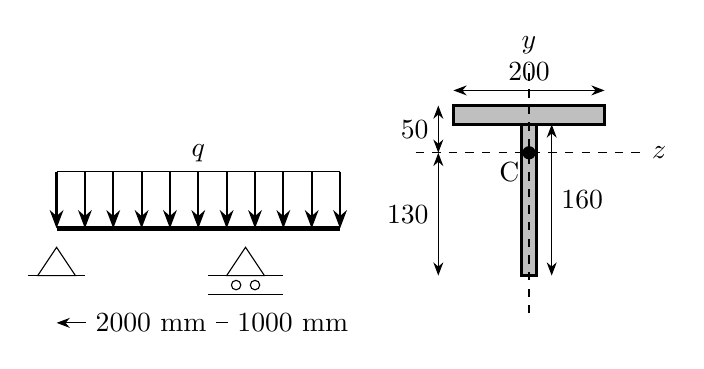
\begin{tikzpicture}[scale=1.2, >=Stealth]
    % Beam axis and loads
    \draw [line width=2.0pt] (0,0) -- (3,0);
    \draw (0,-0.2) -- (0.2,-0.5) -- (-0.2,-0.5) -- cycle;
    \draw (-0.3,-0.5) -- (0.3,-0.5);
    
    \draw (2,-0.2) -- (2.2,-0.5) -- (1.8,-0.5) -- cycle;
    \draw (1.6,-0.5) -- (2.4,-0.5);
    \draw [fill=white] (1.9,-0.6) circle (0.05);
    \draw [fill=white] (2.1,-0.6) circle (0.05);
    \draw (1.6,-0.7) -- (2.4,-0.7);
    
    \foreach \x in {0,0.3,0.6,0.9,1.2,1.5,1.8,2.1,2.4,2.7,3}
        \draw [->, line width=0.8pt] (\x, 0.6) -- (\x, 0);
    \draw (0,0.6) -- (3,0.6);
    \node [above] at (1.5,0.6) {$q$};
    
    \draw [<->] (0,-1) -- (2,-1) node[midway, fill=white] {$2000\text{ mm}$};
    \draw [<->] (2,-1) -- (3,-1) node[midway, fill=white] {$1000\text{ mm}$};
    
    % T-section on the right
    \begin{scope}[xshift=5cm, yshift=-0.5cm, scale=0.8]
        \draw [line width=1.2pt, fill=lightgray] (-1, 2.0) rectangle (1, 2.25);
        \draw [line width=1.2pt, fill=lightgray] (-0.1, 0) rectangle (0.1, 2.0);
        \draw [dashed] (-1.5, 1.625) -- (1.5, 1.625) node[right] {$z$};
        \draw [dashed] (0, -0.5) -- (0, 2.8) node[above] {$y$};
        \draw [fill=black] (0, 1.625) circle (0.08);
        \node [below left] at (0, 1.625) {C};
        
        \draw [<->] (-1.2, 0) -- (-1.2, 1.625) node[midway, left] {$130$};
        \draw [<->] (-1.2, 1.625) -- (-1.2, 2.25) node[midway, left] {$50$};
        \draw [<->] (-1, 2.45) -- (1, 2.45) node[midway, above] {$200$};
        \draw [<->] (0.3, 0) -- (0.3, 2.0) node[midway, right] {$160$};
    \end{scope}
\end{tikzpicture}
\end{center}

\subsubsection*{解答：}

\textbf{1. 梁的内力计算} \\
计算支座反力，设左端支座为 A，右端支座为 B，悬臂端为 D。
梁的总长度为 $3\text{ m}$，受均布载荷 $q = 20\text{ kN/m}$。
\begin{itemize}
    \item 对支座 A 列弯矩平衡：
          \[
              R_B \cdot 2 - q \cdot 3 \cdot 1.5 = 0 \implies R_B = 45\text{ kN}
          \]
    \item 垂直方向力平衡：
          \[
              R_A + R_B = q \cdot 3 \implies R_A = 15\text{ kN}
          \]
\end{itemize}
绘制弯矩图，确定控制截面的弯矩值：
\begin{itemize}
    \item \textbf{最大负弯矩}（位于支座截面 B 处）：
          \[
              M_B = -\frac{1}{2} q \cdot 1^2 = -10\text{ kNm} = -1.0 \times 10^7\text{ Nmm}
          \]
    \item \textbf{最大正弯矩}（位于 AB 跨内剪力为 0 的截面 $x_0$ 处）：
          \[
              V(x_0) = R_A - q x_0 = 0 \implies x_0 = \frac{15}{20} = 0.75\text{ m}
          \]
          \[
              M_{\max} = R_A x_0 - \frac{1}{2} q x_0^2 = 15 \times 0.75 - 10 \times 0.75^2 = 5.625\text{ kNm} = 5.625 \times 10^6\text{ Nmm}
          \]
\end{itemize}

\textbf{2. 截面正应力强度校核} \\
T形截面形心距底边为 $130\text{ mm}$，距顶边为 $50\text{ mm}$。截面关于形心的惯性矩 $I_z = 2.136 \times 10^7\text{ mm}^4$。
\begin{itemize}
    \item \textbf{跨中最大正弯矩截面处}（$M = 5.625\text{ kNm}$，下侧拉伸，上侧压缩）：
          \begin{itemize}
              \item 最大拉应力（下边缘）：
                    \[
                        \sigma_t = \frac{M \cdot y_{\text{bottom}}}{I_z} = \frac{5.625 \times 10^6 \times 130}{2.136 \times 10^7} \approx 34.23\text{ MPa} \le [\sigma]^+ = 35\text{ MPa} \quad (\text{安全})
                    \]
              \item 最大压应力（上边缘）：
                    \[
                        \sigma_c = \frac{M \cdot y_{\text{top}}}{I_z} = \frac{5.625 \times 10^6 \times 50}{2.136 \times 10^7} \approx 13.17\text{ MPa} \le [\sigma]^- = 60\text{ MPa} \quad (\text{安全})
                    \]
          \end{itemize}
    \item \textbf{支座 B 处负弯矩截面处}（$M = -10\text{ kNm}$，上侧拉伸，下侧压缩）：
          \begin{itemize}
              \item 最大拉应力（上边缘）：
                    \[
                        \sigma_t = \frac{|M| \cdot y_{\text{top}}}{I_z} = \frac{1.0 \times 10^7 \times 50}{2.136 \times 10^7} \approx 23.41\text{ MPa} \le [\sigma]^+ = 35\text{ MPa} \quad (\text{安全})
                    \]
              \item 最大压应力（下边缘）：
                    \[
                        \sigma_c = \frac{|M| \cdot y_{\text{bottom}}}{I_z} = \frac{1.0 \times 10^7 \times 130}{2.136 \times 10^7} \approx \mathbf{60.86\text{ MPa}} > [\sigma]^- = 60\text{ MPa} \quad (\mathbf{\text{超标，不安全}})
                    \]
          \end{itemize}
\end{itemize}
\textbf{结论}：由于在支座 B 处下边缘的弯曲压应力达到 $60.86\text{ MPa}$，超过了铸铁材料的抗压许用应力 $60\text{ MPa}$，因此\textbf{该梁不安全}。

---

\section*{3. 卡氏定理求解平面刚架位移}

\textbf{平面刚架受力如图所示，其中横杆和竖杆的弯曲刚度 $EI$、载荷集度 $q$、长度 $l$ 等均为已知。若忽略剪力和轴力的影响，试用卡氏第二定理求竖杆 AB 的中点 D 的水平位移。(25 分)}

\begin{center}
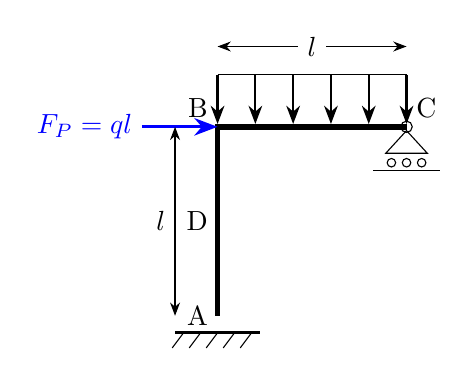
\begin{tikzpicture}[scale=1.2, >=Stealth]
    \draw[line width=2.0pt] (0,0) coordinate(A) -- (0,2) coordinate(B) -- (2,2) coordinate(C);

    \draw[line width=1.2pt] (-0.45,-0.18) -- (0.45,-0.18);
    \foreach \x in {-0.36,-0.18,0,0.18,0.36}
        \draw (\x,-0.18) -- (\x-0.12,-0.34);

    \draw (C) circle (0.06);
    \draw (1.78,1.72) -- (2.22,1.72) -- (2,1.96) -- cycle;
    \foreach \x in {1.84,2.0,2.16}
        \draw[fill=white] (\x,1.62) circle (0.045);
    \draw (1.65,1.54) -- (2.35,1.54);

    \node[left] at (A) {A};
    \node[above left] at (B) {B};
    \node[above right] at (C) {C};
    \node[left] at (0,1) {D};

    \draw[->, line width=1.2pt, blue] (-0.8,2.0) -- (0,2.0);
    \node[left, blue] at (-0.8,2.0) {$F_P=ql$};

    \foreach \x in {0,0.4,0.8,1.2,1.6,2.0}
        \draw[->, thick] (\x,2.55) -- (\x,2.03);
    \draw (0,2.55) -- (2,2.55);
    \node[above] at (1,2.55) {$q$};

    \draw[<->] (-0.45,0) -- (-0.45,2) node[midway, left] {$l$};
    \draw[<->] (0,2.85) -- (2,2.85) node[midway, fill=white] {$l$};
\end{tikzpicture}
\end{center}

\subsubsection*{解答：}

题图中 A 端固支，C 点为竖向滚支，结构为一次超静定刚架。取 C 点竖向反力 $R_C$ 为多余未知力，规定向上为正；竖杆 AB 取坐标 $y$ 自 A 向 B，横杆 BC 取坐标 $x$ 自 B 向 C。

\textbf{1. 由变形协调求 $R_C$}

撤去 C 点竖向支承，得到 A 端固支的基本结构。实际载荷作用下的弯矩为
\[
    M_{AB}(y)=ql(l-y)+R_C l-\frac12ql^2\qquad(0\le y\le l),
\]
\[
    M_{BC}(x)=R_C(l-x)-\frac12q(l-x)^2\qquad(0\le x\le l).
\]
C 点竖向位移为零，由卡氏第二定理得
\[
\frac{\partial U}{\partial R_C}
=\frac1{EI}\left[
\int_0^l M_{AB}l\diff y+
\int_0^l M_{BC}(l-x)\diff x
\right]=0.
\]
代入上式：
\[
\int_0^l\left[ql(l-y)+R_C l-\frac12ql^2\right]l\diff y
+\int_0^l\left[R_C(l-x)-\frac12q(l-x)^2\right](l-x)\diff x=0,
\]
故
\[
    R_C=\frac{3}{32}ql.
\]

\textbf{2. D 点单位水平力体系}

在 D 点沿所求位移正方向施加水平向右单位力。单位体系中 C 点竖向反力增量记为 $r_C$，对应单位弯矩为
\[
    m_{AB}(y)=
    \begin{cases}
        \dfrac l2-y+r_C l, & 0\le y\le \dfrac l2,\\[4pt]
        r_C l, & \dfrac l2\le y\le l,
    \end{cases}
    \qquad
    m_{BC}(x)=r_C(l-x).
\]
同样由 C 点竖向位移协调：
\[
\int_0^l m_{AB}\,l\diff y+\int_0^l m_{BC}(l-x)\diff x=0,
\]
解得
\[
    r_C=-\frac{3}{32}.
\]

\textbf{3. D 点水平位移}

将 $R_C=3ql/32$ 代回实际弯矩，作莫尔积分：
\[
\begin{aligned}
u_D
&=\frac1{EI}\left[
\int_0^l M_{AB}m_{AB}\diff y+
\int_0^l M_{BC}m_{BC}\diff x
\right]\\
&=\frac1{EI}\left[
\frac{137}{3072}ql^4+\frac{9}{1024}ql^4
\right]
=\frac{41ql^4}{768EI}.
\end{aligned}
\]
单位力取向右，结果为正，故
\[
    u_D=\frac{41ql^4}{768EI}\quad(\text{向右}).
\]
---

\section*{4. 细长压杆临界荷载比较}

\textbf{图示两根细长压杆的长度、横截面面积和材料均相同，若 B 杆的内外径之比为 $d_2/D_2 = 0.6$，求两杆临界压力的比值 $P_A : P_B$。(25 分)}

\subsubsection*{解答：}

\textbf{1. 截面惯性矩计算} \\
设两杆截面面积为 $A$。
\begin{itemize}
    \item A杆为实心圆截面，直径为 $D_1$：
          \[
              A_A = \frac{\pi}{4} D_1^2 \implies I_A = \frac{\pi}{64} D_1^4 = \frac{A^2}{4\pi}
          \]
    \item B杆为空心圆截面，外径 $D_2$，内径 $d_2$，内外径比 $\alpha = d_2/D_2 = 0.6$：
          \[
              A_B = \frac{\pi}{4} D_2^2(1 - \alpha^2) \implies D_2^2 = \frac{4 A}{\pi (1 - \alpha^2)}
          \]
          \[
              I_B = \frac{\pi}{64} D_2^4(1 - \alpha^4) = \frac{\pi}{64} \left[ \frac{4 A}{\pi (1 - \alpha^2)} \right]^2 (1 - \alpha^4) = \frac{A^2}{4\pi} \cdot \frac{1 - \alpha^4}{(1 - \alpha^2)^2} = \frac{A^2}{4\pi} \cdot \frac{1 + \alpha^2}{1 - \alpha^2}
          \]
\end{itemize}
代入 $\alpha = 0.6$ 计算两杆的惯性矩之比：
\[
    \frac{I_A}{I_B} = \frac{1 - \alpha^2}{1 + \alpha^2} = \frac{1 - 0.36}{1 + 0.36} = \frac{0.64}{1.36} = \frac{8}{17} \approx 0.471
\]

\textbf{2. 临界力比值分析} \\
根据图示约束，A 杆为两端铰支压杆，取有效长度系数 $\mu_A=1$；B 杆为一端固定、一端铰支导向压杆，取有效长度系数 $\mu_B=0.7$。
由欧拉公式
\[
    P_{\text{cr}}=\frac{\pi^2 E I}{(\mu L)^2},
\]
在两杆长度和材料相同的条件下有
\[
    \frac{P_A}{P_B}
    = \frac{I_A}{I_B}\left(\frac{\mu_B}{\mu_A}\right)^2
    = \frac{8}{17}\times 0.7^2
    \approx 0.231 .
\]
因此两杆临界压力的比值为
\[
    P_A:P_B \approx 0.231:1.
\]


}

\chapter{2004 年期中（1）与秋季工程力学期中解答}
{
\renewcommand{\assetdir}{../../考题_按知识点整理/visual_assets/question_crops/2004_2004年期中_1}



\section*{一、由挠度方程反求载荷、支反力与最大正应力位置}

\begin{center}
    \includegraphics[width=0.92\linewidth]{\assetdir/q-001.png}
\end{center}

题给
\[
    w(x)=\frac{q_0L^4}{840EI}
    \left[
      \left(\frac{x}{L}\right)^7
      -7\left(\frac{x}{L}\right)^3
      +6\frac{x}{L}
    \right].
\]
由梁的微分关系
\[
    EI\,w^{(4)}(x)=q(x)
\]
得
\[
    q(x)=q_0\left(\frac{x}{L}\right)^3,\qquad 0\le x\le L.
\]
故分布载荷为沿梁长按三次方增长的向下载荷，且 $q(L)=q_0$。

载荷合力
\[
    W=\int_0^L q_0\left(\frac{x}{L}\right)^3\,dx=\frac{q_0L}{4},
\]
对 A 点取矩：
\[
    B_yL=\int_0^L xq_0\left(\frac{x}{L}\right)^3\,dx
    =\frac{q_0L^2}{5}.
\]
因此
\[
    B_y=\frac{q_0L}{5},\qquad
    A_y=W-B_y=\frac{q_0L}{20}.
\]

弯矩函数也可由
\[
    M(x)=-EI\,w''(x)
\]
求得：
\[
    M(x)=\frac{q_0L^2}{20}
    \left[
      \frac{x}{L}-\left(\frac{x}{L}\right)^5
    \right].
\]
最大弯矩满足
\[
    F_Q(x)=\frac{dM}{dx}
    =\frac{q_0L}{20}
      \left[
        1-5\left(\frac{x}{L}\right)^4
      \right]=0,
\]
即
\[
    x=\frac{L}{\sqrt[4]{5}}.
\]
横梁为等截面工字形时，最大正应力出现在弯矩绝对值最大截面。故最大正应力位置为
\[
    x=\frac{L}{\sqrt[4]{5}},
\]
截面上的拉伸边缘为最大正应力点。


% \newpage removed


\section*{二、缆车悬臂 AB 与 CD 段最大正应力}

\begin{center}
    \includegraphics[width=0.92\linewidth]{\assetdir/q-002.png}
\end{center}

设车厢和游客总重
\[
    W=5000\text{ N}.
\]
按题图，A、E 两点为铰接，车厢重量通过 A 点作用；E 点支承反力竖直向上。AB 段与载荷作用线重合，CD 段相对 A、E 的竖直作用线有偏心距
\[
    e=0.38\text{ m}.
\]
方形截面边长
\[
    a=0.04\text{ m},
\]
故
\[
    A=a^2=1.6\times10^{-3}\text{ m}^2,\qquad
    W_z=\frac{a^3}{6}=1.0667\times10^{-5}\text{ m}^3.
\]

AB 段只承受轴向力，最大正应力大小为
\[
    \sigma_{AB,\max}=\frac{W}{A}
    =\frac{5000}{1.6\times10^{-3}}
    =3.13\text{ MPa}.
\]

CD 段同时承受轴向力和由偏心距 $e$ 引起的弯矩
\[
    M_{CD}=We=5000\times0.38=1900\text{ N}\cdot\text{m}.
\]
弯曲正应力最大值为
\[
    \sigma_{b,\max}=\frac{M_{CD}}{W_z}
    =\frac{1900}{1.0667\times10^{-5}}
    =178.1\text{ MPa}.
\]
叠加轴向应力，CD 段最大拉应力为
\[
    \sigma_{CD,\max}
    =
    \frac{W}{A}+\frac{M_{CD}}{W_z}
    =3.13+178.1
    =181.3\text{ MPa}.
\]
另一侧边缘为
\[
    \sigma_{CD,\min}=3.13-178.1=-175.0\text{ MPa}.
\]
因此 CD 段控制，最大正应力大小约为 $181\text{ MPa}$。


% \newpage removed


\section*{三、三角形分布载荷外伸梁的内力与挠度积分方程}

\begin{center}
    \includegraphics[width=0.92\linewidth]{\assetdir/q-003.png}
\end{center}

取 A 点为原点，向右为 $x$ 正方向：
\[
    A:0,\qquad B:L,\qquad C:\frac{4L}{3},\qquad D:\frac{5L}{3}.
\]
AB 段载荷为
\[
    q(x)=q_0\frac{x}{L},\qquad 0\le x\le L.
\]
三角形分布载荷合力为 $q_0L/2$，作用点距 A 为 $2L/3$。由整体平衡：
\[
    R_A+R_D=\frac{q_0L}{2}+P,
\]
\[
    R_D\frac{5L}{3}
    =
    \frac{q_0L}{2}\frac{2L}{3}
    +P\frac{4L}{3}.
\]
故
\[
    R_D=\frac{q_0L}{5}+\frac{4P}{5},\qquad
    R_A=\frac{3q_0L}{10}+\frac{P}{5}.
\]

剪力方程为
\[
F_Q(x)=
\begin{cases}
R_A-\dfrac{q_0x^2}{2L},&0\le x\le L,\\[6pt]
R_A-\dfrac{q_0L}{2},&L\le x\le \dfrac{4L}{3},\\[6pt]
R_A-\dfrac{q_0L}{2}-P,&\dfrac{4L}{3}\le x\le \dfrac{5L}{3}.
\end{cases}
\]
也就是
\[
F_Q(x)=
\begin{cases}
\dfrac{3q_0L}{10}+\dfrac{P}{5}-\dfrac{q_0x^2}{2L},&0\le x\le L,\\[6pt]
\dfrac{P-q_0L}{5},&L\le x\le \dfrac{4L}{3},\\[6pt]
-\dfrac{q_0L+4P}{5},&\dfrac{4L}{3}\le x\le \dfrac{5L}{3}.
\end{cases}
\]

弯矩方程为
\[
M(x)=
\begin{cases}
R_Ax-\dfrac{q_0x^3}{6L},&0\le x\le L,\\[6pt]
R_Ax-\dfrac{q_0L}{2}\left(x-\dfrac{2L}{3}\right),
&L\le x\le \dfrac{4L}{3},\\[6pt]
R_D\left(\dfrac{5L}{3}-x\right),
&\dfrac{4L}{3}\le x\le \dfrac{5L}{3}.
\end{cases}
\]
关键弯矩值为
\[
    M(0)=0,\qquad
    M(L)=\frac{2q_0L^2}{15}+\frac{PL}{5},
\]
\[
    M\left(\frac{4L}{3}\right)
    =\frac{q_0L^2}{15}+\frac{4PL}{15},\qquad
    M\left(\frac{5L}{3}\right)=0.
\]
据此即可画出剪力图和弯矩图：AB 段剪力为二次曲线、弯矩为三次曲线；BC 段剪力为常数、弯矩为直线；C 点剪力向下突跳 $P$；CD 段剪力为常数、弯矩线性降至 D 点零值。

挠度积分方程取
\[
    EI\,w''(x)=-M(x).
\]
分段写为
\[
EI\,w_1''=-\left(R_Ax-\frac{q_0x^3}{6L}\right),
\qquad 0\le x\le L,
\]
\[
EI\,w_2''=-\left[
R_Ax-\frac{q_0L}{2}\left(x-\frac{2L}{3}\right)
\right],
\qquad L\le x\le \frac{4L}{3},
\]
\[
EI\,w_3''=-R_D\left(\frac{5L}{3}-x\right),
\qquad \frac{4L}{3}\le x\le \frac{5L}{3}.
\]
边界条件与连续条件为
\[
    w_1(0)=0,\qquad w_3\left(\frac{5L}{3}\right)=0,
\]
\[
    w_1(L)=w_2(L),\qquad w_1'(L)=w_2'(L),
\]
\[
    w_2\left(\frac{4L}{3}\right)=w_3\left(\frac{4L}{3}\right),
    \qquad
    w_2'\left(\frac{4L}{3}\right)=w_3'\left(\frac{4L}{3}\right).
\]


% \newpage removed


\section*{四、L 型圆形截面悬臂梁 D、E 点应力}

\begin{center}
    \includegraphics[width=0.92\linewidth]{\assetdir/q-004.png}
\end{center}

距固定端 $15\text{ cm}$ 的截面到弯折点 B 的距离为
\[
    a=20\text{ cm}=0.20\text{ m},
\]
短梁 $BC$ 长度为
\[
    b=7.5\text{ cm}=0.075\text{ m}.
\]
圆截面直径为
\[
    d=3\text{ cm}=0.03\text{ m}.
\]
截面系数为
\[
    W=\frac{\pi d^3}{32}=2.6507\times10^{-6}\text{ m}^3,
\qquad
    W_p=\frac{\pi d^3}{16}=5.3014\times10^{-6}\text{ m}^3.
\]

将外力分解为垂直于 L 型梁平面的分力和梁平面内分力：
\[
    F_n=F\cos45^\circ=63.64\text{ N},\qquad
    F_p=F\sin45^\circ=63.64\text{ N}.
\]
目标截面轴力为零。对 D、E 两点起作用的弯矩和扭矩取为
\[
    M=F_pa=63.64\times0.20=12.728\text{ N}\cdot\text{m},
\]
\[
    T=F_nb=63.64\times0.075=4.773\text{ N}\cdot\text{m}.
\]
因此弯曲正应力大小为
\[
    \sigma_b=\frac{M}{W}
    =\frac{12.728}{2.6507\times10^{-6}}
    =4.80\text{ MPa}.
\]
扭转切应力大小为
\[
    \tau_T=\frac{T}{W_p}
    =\frac{4.773}{5.3014\times10^{-6}}
    =0.900\text{ MPa}.
\]

按题图 D 点在上侧、E 点在下侧，取本文符号约定，可写为
\[
    \sigma_{xx}(D)=+4.80\text{ MPa},\qquad
    \tau_{xy}(D)=-0.900\text{ MPa},
\]
\[
    \sigma_{xx}(E)=-4.80\text{ MPa},\qquad
    \tau_{xy}(E)=+0.900\text{ MPa}.
\]
两点均为平面应力状态，未列出的面内正应力取零：
\[
    \sigma_{yy}(D)=\sigma_{yy}(E)=0.
\]


}

\chapter{2005 材力期中试题解答}
{
\renewcommand{\assetdir}{../../考题_按知识点整理/visual_assets/question_crops/2005_2005材力期中试题}



\section*{1. 移动集中载荷作用下外伸梁的剪力和弯矩}

\textbf{1．如图所示，某人体重为$P$，从梁的A端走向B端。试写出他在任意位置$x$时，梁的剪力和弯矩表达式；求出当弯矩取最大值时该人所在的位置，并画出相应的剪力图和弯矩图。(25分)}

\begin{center}
    \includegraphics[width=0.92\linewidth]{\assetdir/q-001.png}
\end{center}

取 A 点为坐标原点，梁轴坐标记为 $y$，右侧支座为 C，故
\[
    A: y=0,\qquad C:y=2l,\qquad B:y=3l.
\]
人体重 $P$ 作用于 $y=x$ 处，$0\le x\le 3l$。由整体平衡得
\[
    R_A+R_C=P,\qquad R_C\cdot 2l=Px,
\]
因此
\[
    R_A=P\left(1-\frac{x}{2l}\right),\qquad
    R_C=\frac{Px}{2l}.
\]

\subsection*{人位于 A、C 之间：$0\le x\le 2l$}

\[
Q(y)=
\begin{cases}
P\left(1-\dfrac{x}{2l}\right),&0<y<x,\\[4pt]
-\dfrac{Px}{2l},&x<y<2l,\\[4pt]
0,&2l<y<3l,
\end{cases}
\]
\[
M(y)=
\begin{cases}
P\left(1-\dfrac{x}{2l}\right)y,&0<y<x,\\[4pt]
Px\left(1-\dfrac{y}{2l}\right),&x<y<2l,\\[4pt]
0,&2l<y<3l.
\end{cases}
\]
此时最大弯矩出现在载荷处：
\[
    M_{\max}(x)=Px\left(1-\frac{x}{2l}\right),
    \qquad
    \frac{dM_{\max}}{dx}=P\left(1-\frac{x}{l}\right).
\]
故局部最大值在 $x=l$ 处取得，
\[
    M_{\max,1}=\frac{Pl}{2}.
\]

\subsection*{人位于悬臂段 C、B 之间：$2l<x\le 3l$}

\[
Q(y)=
\begin{cases}
P\left(1-\dfrac{x}{2l}\right),&0<y<2l,\\[4pt]
P,&2l<y<x,\\[4pt]
0,&x<y<3l,
\end{cases}
\]
\[
M(y)=
\begin{cases}
P\left(1-\dfrac{x}{2l}\right)y,&0<y<2l,\\[4pt]
P(y-x),&2l<y<x,\\[4pt]
0,&x<y<3l.
\end{cases}
\]
此时弯矩绝对值最大值发生在 C 截面：
\[
    |M_C|=|P(2l-x)|=P(x-2l).
\]
它随 $x$ 增大而增大，所以全梁、全过程最大弯矩发生在人走到 B 端时：
\[
    x=3l,\qquad |M|_{\max}=Pl,
\]
危险截面为 C 截面。

当 $x=3l$ 时
\[
    R_A=-\frac{P}{2},\qquad R_C=\frac{3P}{2}.
\]
相应剪力图和弯矩图如下。

\begin{figure}[H]
\centering
\begin{tikzpicture}[x=1.75cm,y=0.85cm,>=Latex]
  \draw[->] (-0.15,0) -- (3.35,0) node[right] {$y/l$};
  \draw[->] (0,-0.9) -- (0,1.35) node[above] {$Q/P$};
  \foreach \x/\lab in {0/A,2/C,3/B}{
    \draw[densely dashed,gray] (\x,-0.75)--(\x,1.15);
    \node[below] at (\x,-0.8) {$\lab$};
  }
  \draw[very thick,blue] (0,-0.5)--(2,-0.5);
  \draw[very thick,blue] (2,-0.5)--(2,1);
  \draw[very thick,blue] (2,1)--(3,1);
  \draw[very thick,blue] (3,1)--(3,0);
  \node[left] at (0,-0.5) {$-\dfrac12$};
  \node[above] at (2.5,1) {$1$};

  \begin{scope}[yshift=-4.9cm]
    \draw[->] (-0.15,0) -- (3.35,0) node[right] {$y/l$};
    \draw[->] (0,-1.25) -- (0,0.45) node[above] {$M/(Pl)$};
    \foreach \x/\lab in {0/A,2/C,3/B}{
      \draw[densely dashed,gray] (\x,-1.05)--(\x,0.25);
      \node[below] at (\x,-1.1) {$\lab$};
    }
    \draw[very thick,red] (0,0)--(2,-1)--(3,0);
    \node[left] at (0,0) {$0$};
    \node[below] at (2,-1) {$-1$};
    \node[above] at (3,0) {$0$};
  \end{scope}
\end{tikzpicture}
\caption{题 1 最大弯矩工况的剪力图和弯矩图}
\end{figure}


% \newpage removed


\section*{2. 切槽正方形截面杆的最大正应力}

\textbf{2．正方形截面杆一端固定，另一端自由，中间部分开有切槽。杆自由端受有平行于杆轴线的纵向力$F_P$。若已知$F_P = 1\text{ kN}$，杆各部分尺寸示于图中。试求杆内横截面上的最大正应力，并指出其作用位置。(25分)}

\begin{center}
    \includegraphics[width=0.92\linewidth]{\assetdir/q-002.png}
\end{center}

危险截面取切槽段横截面。由题图，该截面可按 $10\text{ mm}\times10\text{ mm}$ 正方形挖去 $5\text{ mm}\times5\text{ mm}$ 角部槽计算。建立以原正方形左下角为原点的 $y,z$ 坐标。

\subsection*{截面几何性质}

\[
    A=10\times10-5\times5=75\text{ mm}^2,
\]
\[
    \bar y=\bar z
    =\frac{100\cdot5-25\cdot2.5}{75}
    =\frac{35}{6}\text{ mm}.
\]
令
\[
    u=y-\frac{35}{6},\qquad v=z-\frac{35}{6},
\]
并取对角线主轴坐标
\[
    s=\frac{u+v}{\sqrt2},\qquad t=\frac{u-v}{\sqrt2}.
\]
由平行轴定理：
\[
    I_u=I_v=\frac{6875}{12}\text{ mm}^4,\qquad
    I_{uv}=-\frac{625}{3}\text{ mm}^4.
\]
关于 $t$ 轴的主惯性矩为
\[
    I_t=\int_A s^2\,dA
    =\frac{I_u+I_v+2I_{uv}}{2}
    =\frac{4375}{12}\text{ mm}^4.
\]

\subsection*{偏心轴力应力}

轴向力作用线通过未开槽端面的形心 $(5,5)$。相对于切槽截面形心：
\[
    e_s=\frac{\left(5-\frac{35}{6}\right)+\left(5-\frac{35}{6}\right)}{\sqrt2}
    =-\frac{5}{3\sqrt2}\text{ mm},\qquad e_t=0.
\]
按题图箭头，$F_P$ 指向杆内，取拉应力为正时
\[
    N=-F_P=-1000\text{ N}.
\]
于是任一点正应力为
\[
    \sigma=\frac{N}{A}+\frac{Ne_s}{I_t}s
    =-\frac{40}{3}+\frac{16}{7}(u+v)\quad(\text{MPa}).
\]

比较边界顶点即可确定极值：
\[
\begin{array}{c|c|c}
\text{点 }(y,z)\text{ /mm} & u+v\text{ /mm} & \sigma\text{ /MPa}\\
\hline
(5,0) & -\dfrac{20}{3} & -\dfrac{200}{7}\\[3pt]
(10,0) & -\dfrac{5}{3} & -\dfrac{120}{7}\\[3pt]
(10,10) & \dfrac{25}{3} & \dfrac{40}{7}\\[3pt]
(0,10) & -\dfrac{5}{3} & -\dfrac{120}{7}\\[3pt]
(0,5) & -\dfrac{20}{3} & -\dfrac{200}{7}
\end{array}
\]

因此，按题图所示压缩偏心轴力理解时，最大正应力为：
\[
    \sigma_{\max}^{+}=\frac{40}{7}\text{ MPa}=5.71\text{ MPa},
\]
位置在切槽截面的远离槽口外角点 $(10,10)$。同时可见最大压应力为
\[
    \sigma_{\max}^{-}=-\frac{200}{7}\text{ MPa}=-28.57\text{ MPa},
\]
出现在切槽相邻的两个边缘点 $(5,0)$ 和 $(0,5)$，作为压应力校核值。


% \newpage removed


\section*{3. 圆轴拉扭组合下 $45^\circ$ 方向正应变}

\textbf{3．如图所示，已知实心圆轴的直径$d$、弹性模量$E$和泊松比$\nu$，设圆轴在自由端承受外轴向力$P$和外扭转力偶$M = Pd$联合作用。试求在圆轴外表面任意一点沿与纵向线呈 $45^\circ$ 方向的正应变。(25分)}

\begin{center}
    \includegraphics[width=0.92\linewidth]{\assetdir/q-003.png}
\end{center}

圆轴外表面应力为轴向拉应力与扭转切应力叠加。截面面积和抗扭截面系数为
\[
    A=\frac{\pi d^2}{4},\qquad
    W_p=\frac{J_p}{d/2}=\frac{\pi d^3}{16}.
\]
故
\[
    \sigma_x=\frac{P}{A}=\frac{4P}{\pi d^2},\qquad
    \tau_{x\theta}=\frac{M}{W_p}
    =\frac{Pd}{\pi d^3/16}
    =\frac{16P}{\pi d^2}.
\]
圆周向正应力为零，按平面应力广义胡克定律
\[
    \varepsilon_x=\frac{\sigma_x}{E}
    =\frac{4P}{\pi d^2E},\qquad
    \varepsilon_\theta=-\frac{\nu\sigma_x}{E}
    =-\frac{4\nu P}{\pi d^2E}.
\]
又因
\[
    G=\frac{E}{2(1+\nu)},
\]
工程剪应变为
\[
    \gamma_{x\theta}=\frac{\tau_{x\theta}}{G}
    =\frac{32(1+\nu)P}{\pi d^2E}.
\]

沿与轴线成 $45^\circ$ 的方向，按图示正方向取
\[
\begin{aligned}
    \varepsilon_{45^\circ}
    &=\frac{\varepsilon_x+\varepsilon_\theta}{2}
      +\frac{\gamma_{x\theta}}{2}  \\
    &=\frac{2(1-\nu)P}{\pi d^2E}
      +\frac{16(1+\nu)P}{\pi d^2E} \\
    &=\frac{2P}{\pi d^2E}(9+7\nu).
\end{aligned}
\]
若取相反的 $45^\circ$ 方向，则剪应变项变号；本题图中标出的方向对应上式。


% \newpage removed


\section*{4. 正方形截面悬臂梁的最大主应力}

\textbf{4．如图所示，悬臂梁在自由端受集中载荷$F_P$作用，梁的横截面为边长为$b$的正方形，设梁的长度$l = \alpha b$（$\alpha$为给定的无量纲参数）。在考虑剪切应力影响的条件下，求梁的最大主应力，并且指出相应的发生位置和作用面。(25分)}

\begin{center}
    \includegraphics[width=0.92\linewidth]{\assetdir/q-004.png}
\end{center}

最大弯矩和最大剪力均出现在固定端截面：
\[
    M=F_P l=F_P\alpha b,\qquad V=F_P.
\]
设截面形心为原点，$y$ 轴取向拉伸边缘，令
\[
    \eta=\frac{2y}{b},\qquad 0\le \eta\le 1.
\]
正方形截面
\[
    A=b^2,\qquad I=\frac{b^4}{12}.
\]

固定端截面上，弯曲正应力和矩形截面剪应力为
\[
    \sigma_x(\eta)=\frac{My}{I}
    =6\alpha\eta\frac{F_P}{b^2},
\]
\[
    \tau_{xy}(\eta)=\frac{3V}{2A}(1-\eta^2)
    =\frac{3F_P}{2b^2}(1-\eta^2).
\]

该点最大主应力为
\[
\begin{aligned}
    \sigma_1(\eta)
    &=\frac{\sigma_x}{2}
      +\sqrt{\left(\frac{\sigma_x}{2}\right)^2+\tau_{xy}^2} \\
    &=\frac{3F_P}{b^2}
      \left[
      \alpha\eta+
      \sqrt{\alpha^2\eta^2+\frac{(1-\eta^2)^2}{4}}
      \right].
\end{aligned}
\]

最大值只需在固定端截面的拉伸半边 $0\le\eta\le1$ 上求。

\subsection*{较长梁：边缘弯曲正应力控制}

若
\[
    \alpha\ge \sqrt{\frac{2}{27}},
\]
则最大主应力出现在固定端拉伸边缘，即
\[
    \eta=1,\qquad y=\frac b2.
\]
此时剪应力为零，故
\[
    \sigma_{1,\max}=6\alpha\frac{F_P}{b^2}.
\]
最大主应力作用面为固定端横截面，即该主应力方向沿梁轴线。

\subsection*{较短梁：剪应力影响使危险点进入截面内部}

若
\[
    0<\alpha<\sqrt{\frac{2}{27}},
\]
最大主应力出现在固定端拉伸半边内部点
\[
    \eta_0=
    \sqrt{
    \frac{1-3\alpha^2-\sqrt{(1-\alpha^2)(1-9\alpha^2)}}{2}
    },
    \qquad
    y_0=\frac{\eta_0 b}{2}.
\]
最大主应力为
\[
    \sigma_{1,\max}
    =
    \frac{3F_P}{b^2}
    \left[
      \alpha\eta_0+
      \sqrt{\alpha^2\eta_0^2+\frac{(1-\eta_0^2)^2}{4}}
    \right].
\]
最大主应力作用面的法线与梁轴线的夹角 $\theta$ 满足
\[
    \tan 2\theta
    =
    \frac{2\tau_{xy}}{\sigma_x}
    =
    \frac{1-\eta_0^2}{2\alpha\eta_0}.
\]

答题时若题中给出具体 $\alpha$，先与 $\sqrt{2/27}$ 比较；若 $\alpha$ 不小于该值，直接取固定端拉伸外边缘；若 $\alpha$ 小于该值，按上式取内部危险点。


}

\chapter{材料力学 2005 年期末考试试题 (清华大学) 修订解答}
{



\section{选择题}

\begin{enumerate}
\item \textbf{U形截面梁由铸铁制成，若将梁的放置方式由图1(a)改变为图1(b)，则梁的：}
\begin{enumerate}[label=\Alph*.]
    \item 强度、刚度都提高
    \item 强度降低，刚度不变
    \item 强度、刚度都降低
    \item 强度提高，刚度不变
\end{enumerate}

\begin{center}
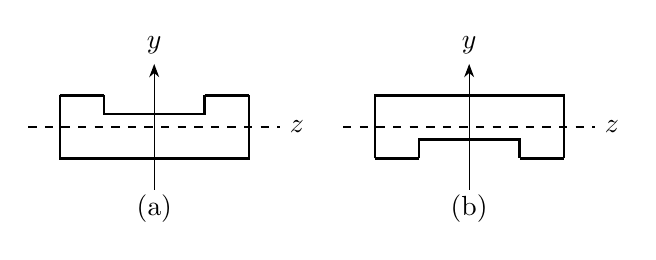
\begin{tikzpicture}[scale=0.8, >=Stealth]
% (a)
\draw[thick] (-1.5,0.5) -- (-1.5,-0.5) -- (1.5,-0.5) -- (1.5,0.5);
\draw[thick] (-0.8,0.5) -- (-0.8,0.2) -- (0.8,0.2) -- (0.8,0.5);
\draw[thick] (-1.5,0.5) -- (-0.8,0.5);
\draw[thick] (0.8,0.5) -- (1.5,0.5);
\draw[dashed] (-2,0) -- (2,0) node[right] {$z$};
\draw[->] (0,-1) -- (0,1) node[above] {$y$};
\node at (0,-1.3) {(a)};

% (b)
\begin{scope}[xshift=5cm]
\draw[thick] (-1.5,-0.5) -- (-1.5,0.5) -- (1.5,0.5) -- (1.5,-0.5);
\draw[thick] (-0.8,-0.5) -- (-0.8,-0.2) -- (0.8,-0.2) -- (0.8,-0.5);
\draw[thick] (-1.5,-0.5) -- (-0.8,-0.5);
\draw[thick] (0.8,-0.5) -- (1.5,-0.5);
\draw[dashed] (-2,0) -- (2,0) node[right] {$z$};
\draw[->] (0,-1) -- (0,1) node[above] {$y$};
\node at (0,-1.3) {(b)};
\end{scope}
\end{tikzpicture}
\par\small 图 1
\end{center}

\textbf{【解答】 正确答案为 B}
\begin{itemize}
    \item \textbf{刚度分析}：梁的弯曲刚度取决于弹性模量 $E$ 和截面惯性矩 $I_z$。由于截面几何形状没有改变，仅仅是绕形心旋转了 $180^\circ$，其绕中性轴 $z$ 的惯性矩 $I_z$ 保持不变。因此，梁的弯曲刚度 $EI_z$ 不变。
    \item \textbf{强度分析}：铸铁是脆性材料，其抗拉强度远低于抗压强度。在向下载荷作用下，梁底弯矩为正，梁下侧受拉，上侧受压。
    对于图(a)（开口朝上），截面重心偏向底部，拉应力侧的距离 $y_t$（中性轴至底部的距离）较小，压应力侧的距离 $y_c$（中性轴至顶部的距离）较大，这样有利于降低最大拉应力值。
    对于图(b)（开口朝下），截面重心偏向顶部，拉应力侧的距离 $y_t$ 变大。根据弯曲正应力公式 $\sigma = M y / I_z$，这会导致底部的最大拉应力增大，使梁的承载能力（强度）显著降低。
\end{itemize}


% \newpage removed


\item \textbf{应力单元体如图2所示，已知斜面 $AB$ 上正应力和切应力均为零，则：}
\begin{enumerate}[label=\Alph*.]
    \item $\sigma_x = \sigma_y, \tau_{xy} = \tau_{yx}$
    \item $\sigma_x \neq \sigma_y, \tau_{xy} \neq \tau_{yx}$
    \item $\sigma_x \neq \sigma_y, \tau_{xy} = \tau_{yx}$
    \item $\sigma_x = \sigma_y, \tau_{xy} \neq \tau_{yx}$
\end{enumerate}

\begin{center}
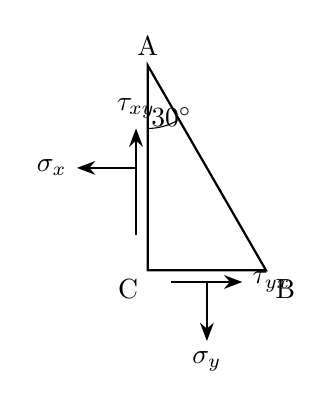
\begin{tikzpicture}[scale=1.5, >=Stealth]
\draw[thick] (0,1.732) coordinate(A) -- (0,0) coordinate(C) -- (1,0) coordinate(B) -- cycle;
\draw (0,1.2) arc (-90:-60:0.5);
\node at (0.2,1.3) {$30^\circ$};
\node[above] at (A) {A};
\node[below left] at (C) {C};
\node[below right] at (B) {B};

% stress arrows
\draw[->, thick] (-0.1, 0.866) -- (-0.6, 0.866) node[left] {$\sigma_x$};
\draw[->, thick] (-0.1, 0.3) -- (-0.1, 1.2) node[above] {$\tau_{xy}$};
\draw[->, thick] (0.5, -0.1) -- (0.5, -0.6) node[below] {$\sigma_y$};
\draw[->, thick] (0.2, -0.1) -- (0.8, -0.1) node[right] {$\tau_{yx}$};
\end{tikzpicture}
\par\small 图 2
\end{center}

\textbf{【解答】 正确答案为 C}
\begin{itemize}
    \item 根据剪应力互等定理，单元体上相互垂直的面上剪应力必然大小相等、方向相对或相反，故恒有 $\tau_{xy} = \tau_{yx}$。
    \item 已知斜面 $AB$（与垂直方向成 $30^\circ$ 角）上正应力和剪应力均为零，这意味着该斜面是一个自由表面，且其法线方向是主应力方向之一，对应的主应力 $\sigma_2 = 0$。另一个主应力 $\sigma_1 \neq 0$ 沿斜面方向。
    \item 由应力状态的变换关系，若设非零主应力为 $\sigma_1$，另一主应力为 0。图中 $AB$ 与竖直边成 $30^\circ$，故 $AB$ 与 $x$ 轴成 $60^\circ$，可取非零主应力方向与 $x$ 轴成 $60^\circ$：
    \[
    \sigma_x = \sigma_1 \cos^2(60^\circ) = \frac{1}{4}\sigma_1,\quad \sigma_y = \sigma_1 \sin^2(60^\circ) = \frac{3}{4}\sigma_1
    \]
    显然 $\sigma_x \neq \sigma_y$。
\end{itemize}

\item \textbf{在圆轴表面点贴应变片如图3所示，当圆轴受到扭转外力偶作用时，应变片\underline{\qquad}的线应变几乎为零。}
\begin{enumerate}[label=\Alph*.]
    \item 1和3
    \item 2
    \item 1和2
    \item 2和3
\end{enumerate}

\begin{center}
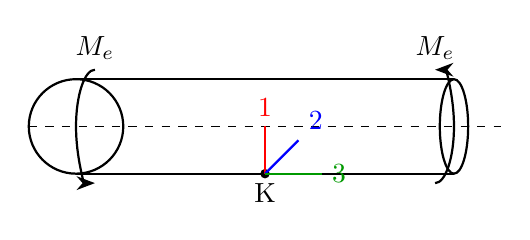
\begin{tikzpicture}[scale=1.2, >=Stealth]
\draw[thick] (0,0.5) -- (4,0.5);
\draw[thick] (0,-0.5) -- (4,-0.5);
\draw[thick] (0,0) circle (0.5);
\draw[thick] (4,0) ellipse (0.15 and 0.5);
\draw[dashed] (-0.5,0) -- (4.5,0);

% torque arrows
\draw[->, thick] (0.2, 0.6) arc (90:270:0.2 and 0.6);
\node[above] at (0.2, 0.6) {$M_e$};
\draw[->, thick] (3.8, -0.6) arc (-90:90:0.2 and 0.6);
\node[above] at (3.8, 0.6) {$M_e$};

% gauges at point K
\coordinate (K) at (2,-0.5);
\fill (K) circle (0.05) node[below] {K};
\draw[thick, red] (K) -- ++(90:0.5) node[above] {1};
\draw[thick, blue] (K) -- ++(45:0.5) node[above right] {2};
\draw[thick, green!60!black] (K) -- ++(0:0.6) node[right] {3};
\end{tikzpicture}
\par\small 图 3
\end{center}

\textbf{【解答】 正确答案为 A}
\begin{itemize}
    \item 圆轴受纯扭转作用时，表面任意点的应力状态为纯剪切状态。在以轴线为 $x$ 轴、横截面切线为 $y$ 轴的坐标系中，正应力 $\sigma_x = \sigma_y = 0$，剪应力 $\tau_{xy} = \tau$。
    \item 沿任意方向 $\theta$ 的线应变为：
    \[
    \varepsilon_\theta = \frac{\varepsilon_x + \varepsilon_y}{2} + \frac{\varepsilon_x - \varepsilon_y}{2}\cos 2\theta + \frac{\gamma_{xy}}{2}\sin 2\theta = \frac{\gamma_{xy}}{2}\sin 2\theta
    \]
    \item 应变片 3 沿轴线方向（$\theta = 0^\circ$），应变片 1 沿横截面切线方向（$\theta = 90^\circ$），因此有 $\varepsilon_{3} = \varepsilon_{0^\circ} = 0$，$\varepsilon_{1} = \varepsilon_{90^\circ} = 0$。应变片 2 沿 $45^\circ$ 方向，线应变为最大主应力方向，不为零。
\end{itemize}
\end{enumerate}


% \newpage removed


\section{计算题}

\begin{enumerate}
\item \textbf{支架如图4所示。载荷 $F = 40\text{ kN}$，三杆的材料相同，$E = 200\text{ GPa}$，各杆横截面面积分别为 $A_1 = 200\text{ mm}^2$，$A_2 = 300\text{ mm}^2$，$A_3 = 400\text{ mm}^2$。试求：(1) 各杆的内力；(2) 节点 A 的位移。}

\begin{center}
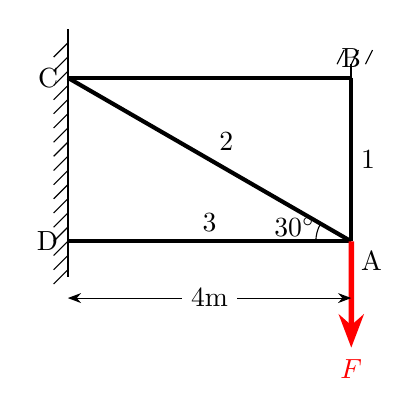
\begin{tikzpicture}[scale=0.9, >=Stealth]
\draw[line width=1.5pt] (0,0) coordinate(D) -- (4,0) coordinate(A);
\draw[line width=1.5pt] (0,2.309) coordinate(C) -- (4,0);
\draw[line width=1.5pt] (4,2.309) coordinate(B) -- (4,0);
\draw[line width=1.5pt] (C) -- (B);

% Wall CD
\draw[thick] (0,-0.5) -- (0,3);
\foreach \y in {-0.4,-0.2,0,0.2,0.4,0.6,0.8,1.0,1.2,1.4,1.6,1.8,2.0,2.2,2.4,2.6,2.8}
  \draw (0,\y) -- (-0.2,\y-0.2);

% Support B
\draw[thick] (4,2.309) -- (4,2.5);
\foreach \x in {3.8,4.0,4.2}
  \draw (\x,2.5) -- (\x+0.1,2.7);

% Labels
\node[left] at (D) {D};
\node[left] at (C) {C};
\node[above] at (B) {B};
\node[below right] at (A) {A};
\node[above] at (2,0) {3};
\node[above right] at (2,1.15) {2};
\node[right] at (4,1.15) {1};

\draw (3.5,0) arc (180:150:0.5);
\node at (3.2,0.2) {$30^\circ$};

% Force F
\draw[->, line width=2pt, red] (A) -- (4,-1.5) node[below] {$F$};

% dimension
\draw[<->] (0,-0.8) -- (4,-0.8) node[midway, fill=white] {4m};
\end{tikzpicture}
\par\small 图 4
\end{center}

\textbf{【解答】}

\textbf{(1) 确定各杆的几何长度}
已知 $l_3 = 4\text{ m}$，由几何关系可知：
\[
l_1 = 4\tan 30^\circ = \frac{4}{\sqrt{3}}\text{ m} \approx 2.309\text{ m}
\]
\[
l_2 = \frac{4}{\cos 30^\circ} = \frac{8}{\sqrt{3}}\text{ m} \approx 4.619\text{ m}
\]

\textbf{(2) 建立平衡方程}
设杆1、杆2受拉为正，杆3受压为正（或由平衡状态可知杆1、2受拉，杆3受压）。对节点 A 进行受力分析：
\[
\sum F_x = F_{N3} - F_{N2}\cos 30^\circ = 0 \implies F_{N3} = F_{N2}\cos 30^\circ \quad \text{--- (1)}
\]
\[
\sum F_y = F_{N1} + F_{N2}\sin 30^\circ - F = 0 \implies F_{N1} + F_{N2}\sin 30^\circ = F \quad \text{--- (2)}
\]

\textbf{(3) 建立变形协调关系}
设节点 A 向左的位移为 $\Delta_x$，向下的位移为 $\Delta_y$。
根据各杆的变形与节点位移的关系：
\begin{align*}
\Delta l_3 &= \Delta_x \quad (\text{杆3缩短}) \\
\Delta l_1 &= \Delta_y \quad (\text{杆1拉伸}) \\
\Delta l_2 &= \Delta_y\sin 30^\circ - \Delta_x\cos 30^\circ \quad (\text{杆2拉伸})
\end{align*}
消除其中的 $\Delta_x$ 和 $\Delta_y$，得到变形协调方程：
\[
\Delta l_1 = \frac{\Delta l_2}{\sin 30^\circ} + \frac{\Delta l_3}{\tan 30^\circ} \quad \text{--- (3)}
\]

\textbf{(4) 物理关系与求解内力}
根据胡克定律，$\Delta l_i = \frac{F_{Ni} l_i}{E A_i}$。将物理关系代入协调方程 (3)：
\[
\frac{F_{N1} l_1}{E A_1} = \frac{F_{N2} l_2}{E A_2 \sin 30^\circ} + \frac{F_{N3} l_3}{E A_3 \tan 30^\circ}
\]
两边消去 $E$，并代入长度和角度关系：
\[
\frac{F_{N1} (4/\sqrt{3})}{A_1} = \frac{F_{N2} (8/\sqrt{3})}{A_2 \cdot 0.5} + \frac{F_{N3} \cdot 4}{A_3 \cdot (1/\sqrt{3})}
\]
简化整理得：
\[
\frac{F_{N1}}{A_1} = \frac{4F_{N2}}{A_2} + \frac{3F_{N3}}{A_3}
\]
代入面积 $A_1=200, A_2=300, A_3=400\text{ mm}^2$：
\[
\frac{F_{N1}}{200} = \frac{4F_{N2}}{300} + \frac{3F_{N3}}{400} \implies 6F_{N1} = 16F_{N2} + 9F_{N3} \quad \text{--- (4)}
\]
联立平衡方程 (1), (2), (4)：
\[
F_{N3} = \frac{\sqrt{3}}{2} F_{N2},\quad F_{N1} = F - 0.5F_{N2}
\]
代入 (4) 中：
\[
6(F - 0.5F_{N2}) = 16F_{N2} + 9\left(\frac{\sqrt{3}}{2} F_{N2}\right) \implies 6F = \left(19 + 4.5\sqrt{3}\right) F_{N2}
\]
代入 $F = 40\text{ kN}$，解得：
\[
F_{N2} = \frac{240}{19 + 4.5\sqrt{3}} \approx 8.96\text{ kN} \quad (\text{受拉})
\]
从而：
\[
F_{N1} = 40 - 0.5 \times 8.96 = 35.52\text{ kN} \approx 35.5\text{ kN} \quad (\text{受拉})
\]
\[
F_{N3} = 8.96 \times \frac{\sqrt{3}}{2} = 7.76\text{ kN} \quad (\text{受压})
\]

\textbf{(5) 计算节点 A 的位移}
\begin{align*}
\Delta_x &= \Delta l_3 = \frac{F_{N3} l_3}{E A_3} = \frac{7.76 \times 10^3 \times 4}{200 \times 10^9 \times 400 \times 10^{-6}} = 0.39\text{ mm} \quad (\text{向左}) \\
\Delta_y &= \Delta l_1 = \frac{F_{N1} l_1}{E A_1} = \frac{35.5 \times 10^3 \times 2.309}{200 \times 10^9 \times 200 \times 10^{-6}} = 2.05\text{ mm} \quad (\text{向下})
\end{align*}
节点 A 的总位移为：
\[
\Delta = \sqrt{\Delta_x^2 + \Delta_y^2} = \sqrt{0.39^2 + 2.05^2} \approx 2.09\text{ mm}
\]
位移方向角（与垂直向下的夹角）：
\[
\theta = \arctan\left(\frac{\Delta_x}{\Delta_y}\right) = \arctan\left(\frac{0.39}{2.05}\right) \approx 10.77^\circ
\]


% \newpage removed


\item \textbf{两端固定的阶梯圆轴，因截面 C 上受到扭动转力偶矩 $M_{ec}$ 的作用。已知 $D_1 = 7\text{ cm}$，$D_2 = 5\text{ cm}$，$[\tau] = 60\text{ MPa}$。试求最大的扭转力偶矩 $M_{ec}$。}

\begin{center}
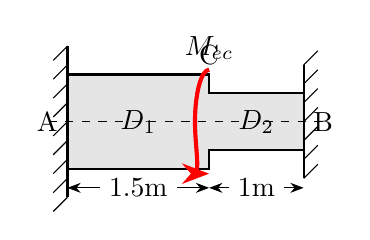
\begin{tikzpicture}[scale=1.2, >=Stealth]
% left support A
\draw[thick] (0,0.8) -- (0,-0.8);
\foreach \y in {-0.8,-0.6,-0.4,-0.2,0,0.2,0.4,0.6,0.8}
  \draw (0,\y) -- (-0.15,\y-0.15);

% right support B
\draw[thick] (2.5,0.6) -- (2.5,-0.6);
\foreach \y in {-0.6,-0.4,-0.2,0,0.2,0.4,0.6}
  \draw (2.5,\y) -- (2.65,\y+0.15);

% shaft AC
\draw[thick, fill=gray!20] (0,0.5) -- (1.5,0.5) -- (1.5,0.3) -- (2.5,0.3) -- (2.5,-0.3) -- (1.5,-0.3) -- (1.5,-0.5) -- (0,-0.5) -- cycle;

% center line
\draw[dashed] (-0.2,0) -- (2.7,0);

% torque at C
\draw[->, line width=1.5pt, red] (1.5,0.55) arc (90:270:0.15 and 0.55);
\node[above] at (1.5,0.55) {$M_{ec}$};

% labels
\node[left] at (0,0) {A};
\node[above] at (1.5,0.5) {C};
\node[right] at (2.5,0) {B};

\draw[<->] (0,-0.7) -- (1.5,-0.7) node[midway, fill=white] {1.5m};
\draw[<->] (1.5,-0.7) -- (2.5,-0.7) node[midway, fill=white] {1m};

\node at (0.75,0) {$D_1$};
\node at (2.0,0) {$D_2$};
\end{tikzpicture}
\par\small 图 5
\end{center}

\textbf{【解答】}

\textbf{(1) 平衡方程}
设 $AC$ 段所受扭矩为 $M_1$，$BC$ 段所受扭矩为 $M_2$，由节点 C 的转动平衡：
\[
M_1 + M_2 = M_{ec} \quad \text{--- (a)}
\]

\textbf{(2) 变形协调条件}
由于两端固定，两段圆轴在 C 截面处的相对转角相等（即 $\varphi_{CA} = \varphi_{CB}$）：
\[
\frac{M_1 l_1}{G I_{p1}} = \frac{M_2 l_2}{G I_{p2}} \implies M_1 = M_2 \frac{l_2}{l_1} \frac{I_{p1}}{I_{p2}}
\]
代入长度与直径：
\[
M_1 = M_2 \frac{1.0}{1.5} \left(\frac{D_1}{D_2}\right)^4 = \frac{2}{3} \left(\frac{7}{5}\right)^4 M_2 \approx 2.56 M_2 \quad \text{--- (b)}
\]

\textbf{(3) 求解段扭矩}
将 (b) 代入 (a) 可得：
\[
M_1 \approx 0.72 M_{ec}, \quad M_2 \approx 0.28 M_{ec}
\]

\textbf{(4) 强度条件约束}
对于 $AC$ 段：
\[
\tau_{1, \max} = \frac{M_1}{W_{p1}} = \frac{0.72 M_{ec}}{\frac{\pi}{16}D_1^3} \le [\tau] \implies M_{ec} \le \frac{60 \times 10^6 \times \frac{\pi}{16} \times 0.07^3}{0.72} \approx 5.6 \times 10^3\text{ N}\cdot\text{m}
\]
对于 $BC$ 段：
\[
\tau_{2, \max} = \frac{M_2}{W_{p2}} = \frac{0.28 M_{ec}}{\frac{\pi}{16}D_2^3} \le [\tau] \implies M_{ec} \le \frac{60 \times 10^6 \times \frac{\pi}{16} \times 0.05^3}{0.28} \approx 5.3 \times 10^3\text{ N}\cdot\text{m}
\]
综合两段的强度要求，取其较小值，以保证全轴安全：
\[
[M_{ec}] = 5.3\text{ kN}\cdot\text{m}
\]


% \newpage removed


\item \textbf{边长为 $a$ 的正方形薄板，两侧面受面分布集度为 $q$ 的均布拉力作用。见图6。已知材料的杨氏弹性模量 $E$ 与泊松比 $\mu$，试求对角线 $AB$ 的伸长。}

\begin{center}
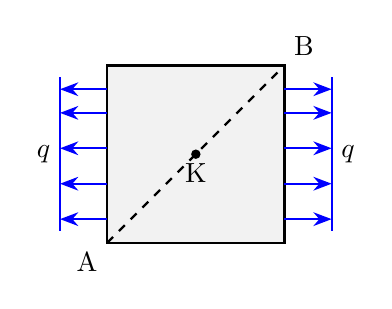
\begin{tikzpicture}[scale=1.5, >=Stealth]
\draw[thick, fill=gray!10] (0,0) coordinate(A) -- (1.5,0) -- (1.5,1.5) coordinate(B) -- (0,1.5) -- cycle;
\draw[thick, dashed] (A) -- (B);
\node[below left] at (A) {A};
\node[above right] at (B) {B};
\node[below] at (0.75,0.75) {K};
\fill (0.75,0.75) circle (0.04);

% tension arrows on left
\foreach \y in {0.2,0.5,0.8,1.1,1.3}
  \draw[->, thick, blue] (0,\y) -- (-0.4,\y);
\draw[thick, blue] (-0.4,0.1) -- (-0.4,1.4);
\node[left] at (-0.4,0.75) {$q$};

% tension arrows on right
\foreach \y in {0.2,0.5,0.8,1.1,1.3}
  \draw[->, thick, blue] (1.5,\y) -- (1.9,\y);
\draw[thick, blue] (1.9,0.1) -- (1.9,1.4);
\node[right] at (1.9,0.75) {$q$};
\end{tikzpicture}
\par\small 图 6
\end{center}

\textbf{【解答】}

\textbf{方法一：主应力法}
\begin{itemize}
    \item 在正方形薄板上取一各面与边界平行的单元体（如 $K$ 点），可知其应力状态为单向受拉：
    \[
    \sigma_x = q,\quad \sigma_y = 0,\quad \tau_{xy} = 0
    \]
    \item 对应对角线 $AB$ 处于与 $x$ 轴成 $45^\circ$ 的方向。由广义胡克定理可先写出 xy 方向的主应变：
    \[
    \varepsilon_x = \frac{q}{E},\quad \varepsilon_y = -\frac{\mu q}{E},\quad \gamma_{xy} = 0
    \]
    \item 根据斜方向线应变计算公式，在 $\theta = 45^\circ$ 的对角线方向上，其线应变 $\varepsilon_{45^\circ}$ 为：
    \[
    \varepsilon_{45^\circ} = \varepsilon_x \cos^2 45^\circ + \varepsilon_y \sin^2 45^\circ = \frac{\varepsilon_x + \varepsilon_y}{2} = \frac{q}{2E}(1 - \mu)
    \]
\end{itemize}

\textbf{方法二：应力圆法}
\begin{itemize}
    \item 绘制该单元体的应力圆，其圆心在 $(q/2, 0)$，半径为 $q/2$。
    \item 旋转 $90^\circ$（物理平面旋转 $45^\circ$）得到对角线 $AB$ 面上的正应力为：
    \[
    \sigma_{45^\circ} = \sigma_{-45^\circ} = \frac{q}{2}
    \]
    \item 同样可由广义胡克定理直接计算该方向线应变：
    \[
    \varepsilon_{45^\circ} = \frac{1}{E}\left(\sigma_{45^\circ} - \mu \sigma_{-45^\circ}\right) = \frac{q}{2E}(1 - \mu)
    \]
\end{itemize}

\textbf{对角线伸长计算}
对角线 $AB$ 的初始几何长度为 $l_{AB} = \sqrt{2}a$，其伸长量 $\Delta l_{AB}$ 为：
\[
\Delta l_{AB} = l_{AB} \cdot \varepsilon_{45^\circ} = \sqrt{2}a \cdot \frac{q}{2E}(1 - \mu) = \frac{\sqrt{2}qa}{2E}(1 - \mu)
\]


% \newpage removed


\item \textbf{偏心的拉伸杆，弹性模量为 $E$，尺寸、受力如图7所示，试求：(1) 最大拉应力和最大压应力的位置和数值；(2) $AB$ 长度的改变量。}

\begin{center}
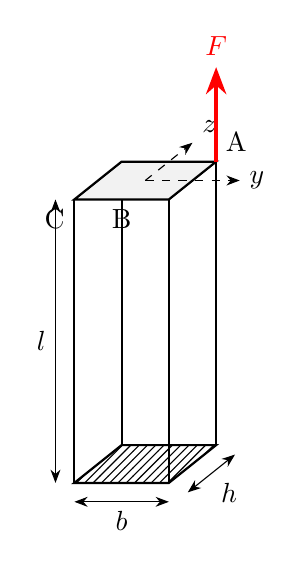
\begin{tikzpicture}[scale=1.2, >=Stealth]
% bottom base
\draw[thick] (0,0) -- (1,0) -- (1.5,0.4) -- (0.5,0.4) -- cycle;
\fill[pattern=north east lines] (0,0) -- (1,0) -- (1.5,0.4) -- (0.5,0.4) -- cycle;

% columns
\draw[thick] (0,0) -- (0,3);
\draw[thick] (1,0) -- (1,3);
\draw[thick] (1.5,0.4) -- (1.5,3.4);
\draw[thick] (0.5,0.4) -- (0.5,3.4);

% top base
\draw[thick, fill=gray!10] (0,3) coordinate(C') -- (1,3) coordinate(B') -- (1.5,3.4) coordinate(A) -- (0.5,3.4) coordinate(C) -- cycle;

% label corners
\node[below left] at (0,3) {C};
\node[above right] at (1.5,3.4) {A};
\node[below] at (0.5,3) {B};

% axes at top centroid
\coordinate (Centroid) at (0.75, 3.2);
\draw[dashed, ->] (Centroid) -- ++(1,0) node[right] {$y$};
\draw[dashed, ->] (Centroid) -- ++(0.5, 0.4) node[above right] {$z$};

% Force F at corner A
\draw[->, line width=1.5pt, red] (A) -- ++(0, 1) node[above] {$F$};

% dimensions
\draw[<->] (-0.2,0) -- (-0.2,3) node[midway, left] {$l$};
\draw[<->] (0,-0.2) -- (1,-0.2) node[midway, below] {$b$};
\draw[<->] (1.2,-0.1) -- (1.7,0.3) node[midway, below right] {$h$};
\end{tikzpicture}
\par\small 图 7
\end{center}

\textbf{【解答】}

\textbf{(1) 偏心拉伸简化与正应力分布}
将偏心拉力 $F$ 向形心轴简化，得到：
\begin{itemize}
    \item 轴向拉力 $F$
    \item 绕 $z$ 轴的弯矩 $M_z = \frac{1}{2} Fb$
    \item 绕 $y$ 轴的弯矩 $M_y = \frac{1}{2} Fh$
\end{itemize}
截面面积 $A = bh$，关于对称轴的弯曲截面系数分别为 $W_z = \frac{1}{6}hb^2$，$W_y = \frac{1}{6}bh^2$。

对于任意点 $(y, z)$，其正应力可表示为：
\[
\sigma(y, z) = \frac{F}{A} + \frac{M_z y}{I_z} + \frac{M_y z}{I_y}
\]
最大应力出现在角点：
\begin{itemize}
    \item \textbf{最大拉应力}出现在偏心力作用侧的角点 A：
    \[
    \sigma_A = \frac{F}{A} + \frac{M_z}{W_z} + \frac{M_y}{W_y} = \frac{F}{bh} + \frac{\frac{1}{2}Fb}{\frac{1}{6}hb^2} + \frac{\frac{1}{2}Fh}{\frac{1}{6}bh^2} = \frac{F}{bh} + 3\frac{F}{bh} + 3\frac{F}{bh} = 7 \frac{F}{bh}
    \]
    \item \textbf{最大压应力}出现在对角线相反侧的角点 C：
    \[
    \sigma_C = \frac{F}{A} - \frac{M_z}{W_z} - \frac{M_y}{W_y} = \frac{F}{bh} - 3\frac{F}{bh} - 3\frac{F}{bh} = -5 \frac{F}{bh}
    \]
\end{itemize}

\textbf{(2) 计算边线 AB 长度的改变量}
由于杆件全长受力恒定，沿着边线 AB 上的各点应力均为最大拉应力 $\sigma_A$。因此其处于单向拉伸状态，线应变为：
\[
\varepsilon_{AB} = \frac{\sigma_A}{E} = 7 \frac{F}{Ebh}
\]
边线 AB 长度的改变值 $\Delta l_{AB}$ 为：
\[
\Delta l_{AB} = \varepsilon_{AB} \cdot l = \frac{7Fl}{Ebh}
\]


% \newpage removed


\item \textbf{试确定图8所示截面的形心位置。}

\begin{center}
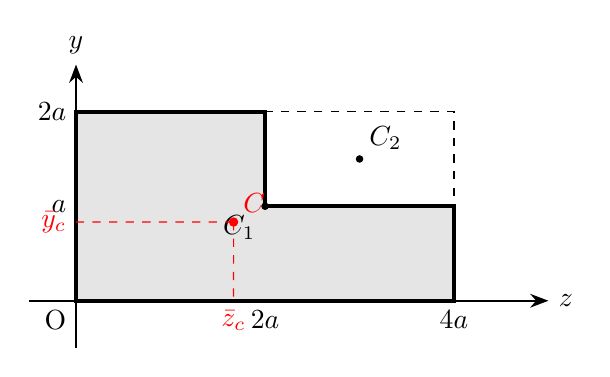
\begin{tikzpicture}[scale=1.2, >=Stealth]
\draw[line width=1.5pt, fill=gray!20] (0,0) -- (4,0) -- (4,1) -- (2,1) -- (2,2) -- (0,2) -- cycle;
\draw[dashed] (2,1) -- (4,1) -- (4,2) -- (2,2) -- cycle;

% axes
\draw[->, thick] (-0.5,0) -- (5,0) node[right] {$z$};
\draw[->, thick] (0,-0.5) -- (0,2.5) node[above] {$y$};

% labels
\node[below left] at (0,0) {O};
\node[below] at (2,0) {$2a$};
\node[below] at (4,0) {$4a$};
\node[left] at (0,1) {$a$};
\node[left] at (0,2) {$2a$};

\coordinate (C1) at (2, 1);
\coordinate (C2) at (3, 1.5);
\fill (C1) circle (0.04) node[below left] {$C_1$};
\fill (C2) circle (0.04) node[above right] {$C_2$};

% centroid of combined shape C
\coordinate (C) at (1.667, 0.833);
\fill[red] (C) circle (0.05) node[above right, red] {$C$};
\draw[dashed, red] (C) -- (1.667, 0) node[below, red] {$\bar{z}_c$};
\draw[dashed, red] (C) -- (0, 0.833) node[left, red] {$\bar{y}_c$};
\end{tikzpicture}
\par\small 图 8
\end{center}

\textbf{【解答】}

\textbf{(1) 采用负面积法（割补法）}
将图示 L 型截面看作是一个完整的大矩形（$4a \times 2a$），割去右上角的一个小矩形（$2a \times a$）而成。

\textbf{(2) 划分单元几何参数}
\begin{itemize}
    \item \textbf{大矩形 (1)}: 
    \begin{align*}
    A_1 &= 4a \times 2a = 8a^2 \\
    \bar{z}_1 &= 2a \\
    \bar{y}_1 &= a
    \end{align*}
    \item \textbf{割去的小矩形 (2)}: 
    \begin{align*}
    A_2 &= 2a \times a = 2a^2 \\
    \bar{z}_2 &= 3a \\
    \bar{y}_2 &= 1.5a
    \end{align*}
\end{itemize}

\textbf{(3) 计算静矩与总面积}
\begin{itemize}
    \item 组合截面的总面积为：
    \[
    A = A_1 - A_2 = 8a^2 - 2a^2 = 6a^2
    \]
    \item 组合截面对 $y$ 轴的静矩 $S_y$ 为：
    \[
    S_y = A_1 \bar{z}_1 - A_2 \bar{z}_2 = (8a^2)(2a) - (2a^2)(3a) = 16a^3 - 6a^3 = 10a^3
    \]
    \item 组合截面对 $z$ 轴的静矩 $S_z$ 为：
    \[
    S_z = A_1 \bar{y}_1 - A_2 \bar{y}_2 = (8a^2)(a) - (2a^2)(1.5a) = 8a^3 - 3a^3 = 5a^3
    \]
\end{itemize}

\textbf{(4) 确定形心位置的坐标}
\[
\bar{z}_c = \frac{S_y}{A} = \frac{10a^3}{6a^2} = \frac{5}{3}a \approx 1.67a
\]
\[
\bar{y}_c = \frac{S_z}{A} = \frac{5a^3}{6a^2} = \frac{5}{6}a \approx 0.83a
\]
因此，形心 $C$ 的坐标位置为 $\left(\frac{5}{3}a, \frac{5}{6}a\right)$。
\end{enumerate}


}

\chapter{材料力学 2005 年期末测验试题 (A) 修订解答}
{



\section*{1. 梁的挠曲线微分方程求解}

\textbf{如图所示，已知：$q$、$EI$、$l$。试根据梁的挠曲线微分方程和约束条件，求梁的挠度曲线表达式。(25 分)}

\begin{center}
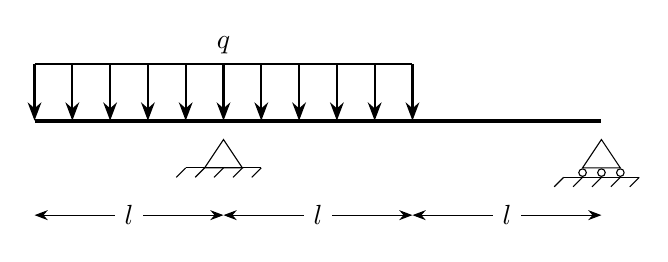
\begin{tikzpicture}[scale=1.2, >=Stealth]
% Beam axis
\draw[line width=1.5pt] (0,0) -- (6,0);

% Supports
\draw (2,-0.2) -- (2.2,-0.5) -- (1.8,-0.5) -- cycle;
\draw (1.6,-0.5) -- (2.4,-0.5);
\foreach \x in {1.6,1.8,2.0,2.2,2.4}
  \draw (\x,-0.5) -- (\x-0.1,-0.6);

\draw (6,-0.2) -- (6.2,-0.5) -- (5.8,-0.5) -- cycle;
\foreach \x in {5.8, 6.0, 6.2}
  \draw[fill=white] (\x,-0.55) circle (0.04);
\draw (5.6,-0.6) -- (6.4,-0.6);
\foreach \x in {5.6,5.8,6.0,6.2,6.4}
  \draw (\x,-0.6) -- (\x-0.1,-0.7);

% Load q
\foreach \x in {0,0.4,0.8,1.2,1.6,2.0,2.4,2.8,3.2,3.6,4.0}
  \draw[->, thick] (\x,0.6) -- (\x,0);
\draw (0,0.6) -- (4,0.6);
\node[above] at (2,0.6) {$q$};

% Dimensions
\draw[<->] (0,-1) -- (2,-1) node[midway, fill=white] {$l$};
\draw[<->] (2,-1) -- (4,-1) node[midway, fill=white] {$l$};
\draw[<->] (4,-1) -- (6,-1) node[midway, fill=white] {$l$};
\end{tikzpicture}
\end{center}

\subsubsection*{解答：}

以梁的最左端为原点 $O$，梁的轴线为 $x$ 轴，设挠度 $w(x)$ 垂直向上为正。

\textbf{1. 确定支反力} \\
设 $x=l$ 处的铰支座反力为 $R_1$，$x=3l$ 处的滚轴支座反力为 $R_2$，均以向上为正。
根据整体静力平衡：
\[
\sum F_y = R_1 + R_2 - 2ql = 0
\]
\[
\sum M_{(x=l)} = R_2 \cdot 2l - q \cdot 2l \cdot 0 = 0 \implies R_2 = 0
\]
由上式可直接解得：
\[
R_2 = 0, \quad R_1 = 2ql
\]

\textbf{2. 分段建立弯矩方程}
\begin{itemize}
    \item \textbf{第一段 ($0 \le x \le l$)}：
    \[
    M_1(x) = -\frac{1}{2}qx^2
    \]
    \item \textbf{第二段 ($l \le x \le 2l$)}：
    \[
    M_2(x) = -\frac{1}{2}qx^2 + R_1(x-l) = -\frac{1}{2}qx^2 + 2ql(x-l)
    \]
    \item \textbf{第三段 ($2l \le x \le 3l$)}：
    \[
    M_3(x) = 0
    \]
\end{itemize}

\textbf{3. 分段积分计算挠曲线表达式}
根据梁的挠曲线微分方程 $EI w''(x) = M(x)$：
\begin{itemize}
    \item \textbf{第一段}：
    \[
    EI w_1''(x) = -\frac{1}{2}qx^2 \implies EI w_1'(x) = -\frac{1}{6}qx^3 + C_1 \implies EI w_1(x) = -\frac{1}{24}qx^4 + C_1 x + D_1
    \]
    \item \textbf{第二段}：
    \[
    EI w_2''(x) = -\frac{1}{2}qx^2 + 2qlx - 2ql^2
    \]
    \[
    EI w_2'(x) = -\frac{1}{6}qx^3 + qlx^2 - 2ql^2 x + C_2
    \]
    \[
    EI w_2(x) = -\frac{1}{24}qx^4 + \frac{1}{3}qlx^3 - ql^2 x^2 + C_2 x + D_2
    \]
    \item \textbf{第三段}：
    \[
    EI w_3''(x) = 0 \implies EI w_3'(x) = C_3 \implies EI w_3(x) = C_3 x + D_3
    \]
\end{itemize}

\textbf{4. 利用边界条件与连续性条件求解常数}
\begin{enumerate}[label=(\arabic*)]
    \item 在 $x=l$ 处位移为零：$w_1(l) = 0 \implies D_1 = \frac{1}{24}ql^4 - C_1 l$。
    \item 在 $x=l$ 处位移连续且为零：$w_2(l) = 0 \implies D_2 = \frac{17}{24}ql^4 - C_2 l$。
    \item 在 $x=l$ 处转角连续：$w_1'(l) = w_2'(l) \implies C_2 = C_1 + ql^3$。
    \item 在 $x=3l$ 处位移为零：$w_3(3l) = 0 \implies D_3 = -3l C_3$。
    \item 在 $x=2l$ 处位移连续：$w_2(2l) = w_3(2l)$。
    \item 在 $x=2l$ 处转角连续：$w_2'(2l) = w_3'(2l)$。
\end{enumerate}

联立以上条件，解得各积分常数分别为：
\[
C_1 = \frac{5}{16}ql^3, \quad D_1 = -\frac{13}{48}ql^4, \quad C_2 = \frac{21}{16}ql^3, \quad D_2 = -\frac{29}{48}ql^4, \quad C_3 = -\frac{1}{48}ql^3, \quad D_3 = \frac{1}{16}ql^4
\]

\textbf{5. 挠度曲线最终表达式}
\[
w(x) = \begin{cases} 
\dfrac{q}{48EI}\left(-2x^4 + 15l^3 x - 13l^4\right) & (0 \le x \le l) \\
\dfrac{q}{48EI}\left(-2x^4 + 16lx^3 - 48l^2 x^2 + 63l^3 x - 29l^4\right) & (l \le x \le 2l) \\
\dfrac{ql^3}{48EI}\left(-x + 3l\right) & (2l \le x \le 3l)
\end{cases}
\]


% \newpage removed


\section*{2. T形截面外伸梁弯曲强度与安全校核}

\textbf{T 形截面外伸梁，受力与截面尺寸如图所示，其中 $C$ 为截面形心，$q=20\text{kN/m}$，$I_z = 2.136 \times 10^7\text{ mm}^4$。梁的材料为铸铁，其抗拉许用应力 $[\sigma]^+ = 35\text{MPa}$，抗压许用应力 $[\sigma]^- = 60\text{MPa}$。试校核该梁是否安全（忽略剪力影响）。(25 分)}

\begin{center}
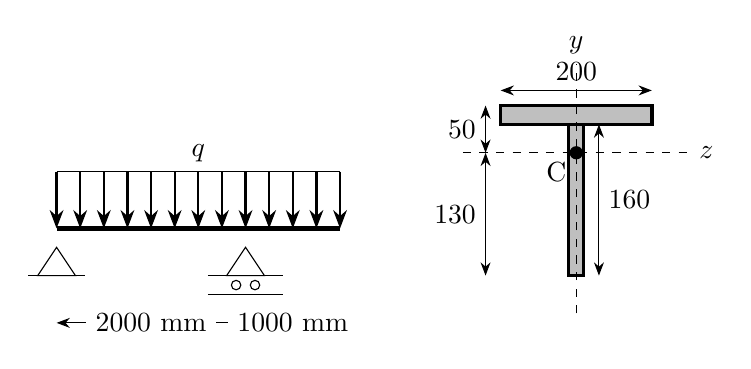
\begin{tikzpicture}[scale=1.2, >=Stealth]
% Beam axis and loads
\draw [line width=2.0pt] (0,0) -- (3,0);
\draw (0,-0.2) -- (0.2,-0.5) -- (-0.2,-0.5) -- cycle;
\draw (-0.3,-0.5) -- (0.3,-0.5);

\draw (2,-0.2) -- (2.2,-0.5) -- (1.8,-0.5) -- cycle;
\draw (1.6,-0.5) -- (2.4,-0.5);
\draw [fill=white] (1.9,-0.6) circle (0.05);
\draw [fill=white] (2.1,-0.6) circle (0.05);
\draw (1.6,-0.7) -- (2.4,-0.7);

\foreach \x in {0,0.25,0.5,0.75,1.0,1.25,1.5,1.75,2.0,2.25,2.5,2.75,3.0}
    \draw [->, line width=0.8pt] (\x, 0.6) -- (\x, 0);
\draw (0,0.6) -- (3,0.6);
\node [above] at (1.5,0.6) {$q$};

\draw [<->] (0,-1) -- (2,-1) node[midway, fill=white] {$2000\text{ mm}$};
\draw [<->] (2,-1) -- (3,-1) node[midway, fill=white] {$1000\text{ mm}$};

% T-section on the right
\begin{scope}[xshift=5.5cm, yshift=-0.5cm, scale=0.8]
    \draw [line width=1.2pt, fill=lightgray] (-1, 2.0) rectangle (1, 2.25);
    \draw [line width=1.2pt, fill=lightgray] (-0.1, 0) rectangle (0.1, 2.0);
    \draw [dashed] (-1.5, 1.625) -- (1.5, 1.625) node[right] {$z$};
    \draw [dashed] (0, -0.5) -- (0, 2.8) node[above] {$y$};
    \draw [fill=black] (0, 1.625) circle (0.08);
    \node [below left] at (0, 1.625) {C};
    
    \draw [<->] (-1.2, 0) -- (-1.2, 1.625) node[midway, left] {$130$};
    \draw [<->] (-1.2, 1.625) -- (-1.2, 2.25) node[midway, left] {$50$};
    \draw [<->] (-1, 2.45) -- (1, 2.45) node[midway, above] {$200$};
    \draw [<->] (0.3, 0) -- (0.3, 2.0) node[midway, right] {$160$};
\end{scope}
\end{tikzpicture}
\end{center}

\subsubsection*{解答：}

\textbf{1. 梁的内力分析}
均布荷载 $q=20\text{ kN/m}$ 作用于梁的全长 $AC=3\text{ m}$，其中 $AB=2\text{ m}$、外伸段 $BC=1\text{ m}$。设左支座为 A，右支座为 B，则
\[
R_A+R_B=q\cdot 3=60\text{ kN},\qquad
\sum M_A=0:\ R_B\cdot2-q\cdot3\cdot1.5=0.
\]
故
\[
R_A=15\text{ kN},\qquad R_B=45\text{ kN}.
\]
在 $AB$ 段内，取 $x$ 自 A 向 B：
\[
V_1(x)=15-20x,\qquad
M_1(x)=15x-10x^2\quad(0\le x\le2),
\]
在外伸段 $BC$ 内：
\[
V_2(x)=60-20x,\qquad
M_2(x)=60x-90-10x^2\quad(2\le x\le3),
\]
其中力单位为 kN、长度单位为 m。令 $V_1=0$ 得正弯矩最大截面
\[
x=0.75\text{ m},\qquad M_{\max}^{+}=5.625\text{ kN}\cdot\text{m}.
\]
B 支座截面处有最大负弯矩
\[
M_B=M_1(2)=M_2(2)=-10\text{ kN}\cdot\text{m}.
\]

\textbf{2. 弯曲正应力计算与校核}
已知形心 $C$ 距离截面底边 $y_{\text{bottom}}=130\text{ mm}$，距离截面顶边 $y_{\text{top}}=50\text{ mm}$，惯性矩 $I_z=2.136\times10^7\text{ mm}^4$。
正弯矩最大截面使下边缘受拉、上边缘受压。下边缘最大拉应力为
\[
\sigma_{t,+}=\frac{M_{\max}^{+}y_{\text{bottom}}}{I_z}
=\frac{5.625\times10^6\times130}{2.136\times10^7}
\approx34.23\text{ MPa}<[\sigma]^+=35\text{ MPa}.
\]
B 截面负弯矩使上边缘受拉、下边缘受压。上边缘拉应力为
\[
\sigma_{t,B}=\frac{|M_B|y_{\text{top}}}{I_z}
=\frac{10\times10^6\times50}{2.136\times10^7}
\approx23.41\text{ MPa}<[\sigma]^+=35\text{ MPa},
\]
下边缘压应力为
\[
\sigma_{c,B}=\frac{|M_B|y_{\text{bottom}}}{I_z}
=\frac{10\times10^6\times130}{2.136\times10^7}
\approx60.86\text{ MPa}>[\sigma]^-=60\text{ MPa}.
\]
\textbf{结论}：B 支座截面下边缘压应力略超过铸铁抗压许用应力，故该梁\textbf{不安全}。


% \newpage removed


\section*{3. 平面刚架位移计算}

\textbf{平面刚架受力如图所示，其中的 $F$、$l$ 以及 $EI$ 等均为已知。若忽略轴力和剪力的影响，试用卡氏第二定理（或莫尔积分法）求 A、B 两点的相对位移 $\Delta_{AB}$。(25 分)}

\begin{center}
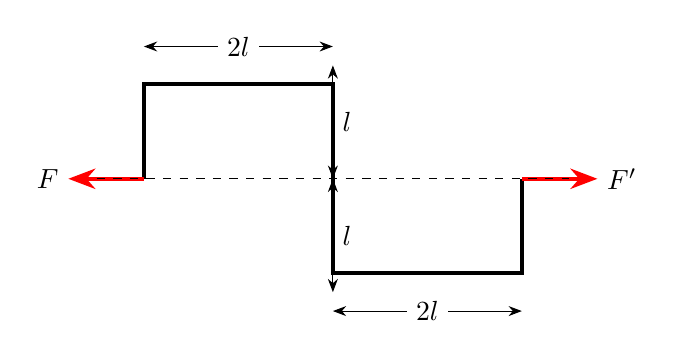
\begin{tikzpicture}[scale=1.2, >=Stealth]
% Draw frame
\draw[line width=1.5pt] (0,0) coordinate(A) -- (0,1) -- (2,1) -- (2,-1) -- (4,-1) -- (4,0) coordinate(B);

% Forces
\draw[->, line width=1.5pt, red] (0,0) -- (-0.8,0);
\node[left] at (-0.8,0) {$F$};

\draw[->, line width=1.5pt, red] (4,0) -- (4.8,0);
\node[right] at (4.8,0) {$F'$};

% Dotted line
\draw[dashed] (-0.5,0) -- (4.5,0);

% Dimensions
\draw[<->] (2,1.2) -- (2,0) node[midway, right] {$l$};
\draw[<->] (2,0) -- (2,-1.2) node[midway, right] {$l$};
\draw[<->] (0,1.4) -- (2,1.4) node[midway, fill=white] {$2l$};
\draw[<->] (2,-1.4) -- (4,-1.4) node[midway, fill=white] {$2l$};
\end{tikzpicture}
\end{center}

\subsubsection*{解答：}

由于结构和外载荷完全自平衡，可以直接利用卡氏第二定理求 A、B 两点沿力方向的相对位移。计算时把右端载荷写成 $F'$，最后令 $F'=F$；等价地，也可以把两端等大反向力看成由同一个参数 $F$ 控制，并对这个共同参数求偏导，所得就是 A、B 两点的相对远离位移 $\Delta_{AB}$。

\textbf{1. 建立分段弯矩方程}
利用结构的对称性，我们可以将结构分成五段进行弯矩计算。设各段弯矩以使构件内侧受拉为正：
\begin{itemize}
    \item \textbf{第一段（左侧外竖直段，长度为 $l$）}：从 A ($y=0$) 到顶部转角 ($y=l$)：
    \[
    M_1(y) = F y \quad (0 \le y \le l)
    \]
    \item \textbf{第二段（左侧水平段，长度为 $2l$）}：自左转角 ($x=0$) 到中节点 ($x=2l$)：
    \[
    M_2(x) = F l \quad (0 \le x \le 2l)
    \]
    \item \textbf{第三段（中间竖直段，长度为 $2l$）}：自顶端 ($y_m=0$) 到底端 ($y_m=2l$)：
    \[
    M_3(y_m) = F(l - y_m) \quad (0 \le y_m \le 2l)
    \]
    \item \textbf{第四段（右侧水平段，长度为 $2l$）}：自中节点 ($x'=0$) 到右转角 ($x'=2l$)：
    \[
    M_4(x') = -F l \quad (0 \le x' \le 2l)
    \]
    \item \textbf{第五段（右侧外竖直段，长度为 $l$）}：从底部转角 ($y'=l$) 到 B ($y'=0$)：
    \[
    M_5(y') = -F y' \quad (0 \le y' \le l)
    \]
\end{itemize}

\textbf{2. 变形能与相对位移计算}
系统的总弯曲变形能为：
\[
U = \sum \int \frac{M^2}{2EI} \diff s = 2 \int_0^l \frac{(Fy)^2}{2EI} \diff y + 2 \int_0^{2l} \frac{(Fl)^2}{2EI} \diff x + \int_0^{2l} \frac{F^2(l - y_m)^2}{2EI} \diff y_m
\]
计算各分项积分：
\begin{align*}
U_{\text{vert, outer}} &= 2 \times \frac{F^2 l^3}{6EI} = \frac{F^2 l^3}{3EI} \\
U_{\text{horiz}} &= 2 \times \frac{F^2 l^3}{EI} = \frac{2F^2 l^3}{EI} \\
U_{\text{vert, mid}} &= \frac{F^2}{2EI} \left[ \frac{(l-y_m)^3}{-3} \right]_0^{2l} = \frac{F^2 l^3}{3EI}
\end{align*}
相加得到总弯曲能：
\[
U = \frac{F^2 l^3}{3EI} + \frac{2F^2 l^3}{EI} + \frac{F^2 l^3}{3EI} = \frac{8 F^2 l^3}{3EI}
\]
由卡氏第二定理，A、B 两点沿力 $F$ 方向的相对位移（即相对远离位移）为：
\[
\Delta_{AB} = \frac{\partial U}{\partial F} = \frac{16 F l^3}{3EI}
\]


% \newpage removed


\section*{4. 结构安全最大载荷计算}

\textbf{图示梁 AB 在 A 端固支、在 C 点与杆 CD 铰接、在 B 点作用集中力 P。设梁 AB 和杆 CD 的横截面均为边长为 $b = a/10$ 的正方形，并且它们具有相同的弹性模量 $E$ 和许用应力 $[\sigma] = 0.5 \times 10^{-3} E$。杆 CD 的稳定安全因数 $[n]_{st} = 1.5$。若忽略剪力影响，试求保证结构安全的最大载荷 P。(25 分)}

\begin{center}
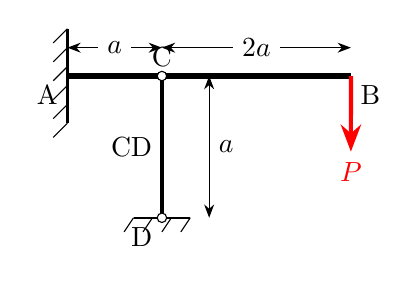
\begin{tikzpicture}[scale=1.2, >=Stealth]
% Wall at A
\draw[thick] (0,-0.5) -- (0,0.5);
\foreach \y in {-0.5,-0.3,-0.1,0.1,0.3,0.5}
  \draw (0,\y) -- (-0.15,\y-0.15);

% Beam AB
\draw[line width=2.0pt] (0,0) coordinate(A) -- (3,0) coordinate(B);

% Rod CD
\draw[line width=1.5pt] (1,0) coordinate(C) -- (1,-1.5) coordinate(D);
\draw[fill=white] (C) circle (0.05);

% Wall at D
\draw[thick] (0.7,-1.5) -- (1.3,-1.5);
\foreach \x in {0.7,0.9,1.1,1.3}
  \draw (\x,-1.5) -- (\x-0.1,-1.65);
\draw[fill=white] (D) circle (0.05);

% Force P
\draw[->, line width=1.5pt, red] (B) -- (3,-0.8) node[below] {$P$};

% Labels
\node[below left] at (A) {A};
\node[above] at (C) {C};
\node[below right] at (B) {B};
\node[left] at (1,-0.75) {CD};
\node[below left] at (D) {D};

% Dimensions
\draw[<->] (0,0.3) -- (1,0.3) node[midway, fill=white] {$a$};
\draw[<->] (1,0.3) -- (3,0.3) node[midway, fill=white] {$2a$};
\draw[<->] (1.5,0) -- (1.5,-1.5) node[midway, right] {$a$};
\end{tikzpicture}
\end{center}

\subsubsection*{解答：}

设杆 CD 顶端对梁 AB 施加的向上支撑力为 $R_C$。杆 CD 本身为两端铰支的受压杆件。

\textbf{1. 求解变形协调关系}
由梁 AB 在 C 点的向下挠度与杆 CD 的轴向压缩量相等：
\begin{itemize}
    \item 集中力 $P$ 引起的 C 点挠度：
    \[
    w_P = \frac{Pa^2}{6EI}(3 \times 3a - a) = \frac{4Pa^3}{3EI}
    \]
    \item 支撑力 $R_C$ 引起的 C 点挠度：
    \[
    w_R = -\frac{R_C a^3}{3EI}
    \]
    \item 杆 CD 自身的弹性压缩量为：
    \[
    \Delta l = \frac{R_C a}{EA_{\text{rod}}} = \frac{R_C a}{E b^2}
    \]
\end{itemize}
由变形协调 $w_P + w_R = \Delta l$ 得：
\[
\frac{4Pa^3}{3EI} - \frac{R_C a^3}{3EI} = \frac{R_C a}{E b^2}
\]
代入截面惯性矩 $I = \frac{b^4}{12}$ 和截面尺寸 $b = a/10$：
\[
\frac{160000 P}{E a} - \frac{40000 R_C}{E a} = \frac{100 R_C}{E a} \implies R_C = \frac{1600}{401}P \approx 3.99 P
\]

\textbf{2. 考虑结构各构件的承载限制条件}
\begin{itemize}
    \item \textbf{限制条件一：梁 AB 的弯曲强度} \\
    梁 AB 的弯矩图在 C 处取最大值 $M_C = 2Pa$。要求：
    \[
    \sigma_{\max} = \frac{M_C}{W} = \frac{2Pa}{\frac{1}{6}b^3} \le [\sigma] \implies \frac{12Pa}{\frac{a^3}{1000}} \le 0.5 \times 10^{-3} E \implies P \le 4.17 \times 10^{-8} Ea^2
    \]
    \item \textbf{限制条件二：杆 CD 的压缩强度} \\
    \[
    \sigma_{CD} = \frac{R_C}{b^2} \le [\sigma] \implies \frac{3.99 P}{\frac{a^2}{100}} \le 0.5 \times 10^{-3} E \implies P \le 1.25 \times 10^{-6} Ea^2
    \]
    \item \textbf{限制条件三：压杆 CD 的稳定安全性} \\
    压杆 CD 两端铰支 ($\mu = 1.0$)，临界载荷由欧拉公式给出：
    \[
    P_{cr} = \frac{\pi^2 EI_{CD}}{a^2} = \frac{\pi^2 E b^4}{12 a^2} = \frac{\pi^2 E a^2}{120000}
    \]
    稳定许用荷载为 $[P]_{st} = \frac{P_{cr}}{[n]_{st}} = \frac{\pi^2 E a^2}{180000}$。要求：
    \[
    R_C \le [P]_{st} \implies 3.99 P \le \frac{\pi^2 E a^2}{180000} \implies P \le 1.37 \times 10^{-5} Ea^2
    \]
\end{itemize}

比较上述三个限制条件，取最小值作为保证结构安全的最大载荷：
\[
P_{\max} = 4.17 \times 10^{-8} Ea^2
\]


}

\chapter{材料力学 2006 年期末测验试题 (A) 修订解答}
{



\section*{1. 梁的挠曲线微分方程求解}

\textbf{如图所示，已知：$q$、$EI$、$l$。试根据梁的挠曲线微分方程和约束条件，求梁的挠度曲线表达式。(25 分)}

\begin{center}
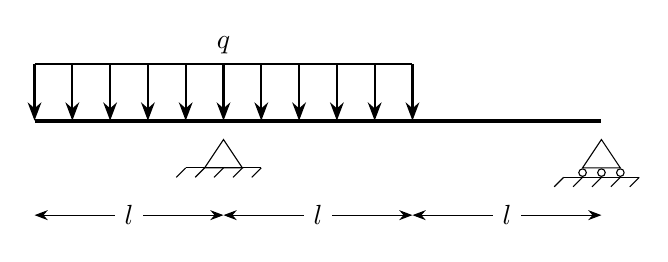
\begin{tikzpicture}[scale=1.2, >=Stealth]
% Beam axis
\draw[line width=1.5pt] (0,0) -- (6,0);

% Supports
\draw (2,-0.2) -- (2.2,-0.5) -- (1.8,-0.5) -- cycle;
\draw (1.6,-0.5) -- (2.4,-0.5);
\foreach \x in {1.6,1.8,2.0,2.2,2.4}
  \draw (\x,-0.5) -- (\x-0.1,-0.6);

\draw (6,-0.2) -- (6.2,-0.5) -- (5.8,-0.5) -- cycle;
\foreach \x in {5.8, 6.0, 6.2}
  \draw[fill=white] (\x,-0.55) circle (0.04);
\draw (5.6,-0.6) -- (6.4,-0.6);
\foreach \x in {5.6,5.8,6.0,6.2,6.4}
  \draw (\x,-0.6) -- (\x-0.1,-0.7);

% Load q
\foreach \x in {0,0.4,0.8,1.2,1.6,2.0,2.4,2.8,3.2,3.6,4.0}
  \draw[->, thick] (\x,0.6) -- (\x,0);
\draw (0,0.6) -- (4,0.6);
\node[above] at (2,0.6) {$q$};

% Dimensions
\draw[<->] (0,-1) -- (2,-1) node[midway, fill=white] {$l$};
\draw[<->] (2,-1) -- (4,-1) node[midway, fill=white] {$l$};
\draw[<->] (4,-1) -- (6,-1) node[midway, fill=white] {$l$};
\end{tikzpicture}
\end{center}

\subsubsection*{解答：}

以梁的最左端为原点 $O$，梁的轴线为 $x$ 轴，设挠度 $w(x)$ 垂直向上为正。

\textbf{1. 确定支反力} \\
设 $x=l$ 处的铰支座反力为 $R_1$，$x=3l$ 处的滚轴支座反力为 $R_2$，均以向上为正。
根据整体静力平衡：
\[
\sum F_y = R_1 + R_2 - 2ql = 0
\]
\[
\sum M_{(x=l)} = R_2 \cdot 2l - q \cdot 2l \cdot 0 = 0 \implies R_2 = 0
\]
解得：
\[
R_2 = 0, \quad R_1 = 2ql
\]

\textbf{2. 分段建立弯矩方程}
\begin{itemize}
    \item \textbf{第一段 ($0 \le x \le l$)}：
    \[
    M_1(x) = -\frac{1}{2}qx^2
    \]
    \item \textbf{第二段 ($l \le x \le 2l$)}：
    \[
    M_2(x) = -\frac{1}{2}qx^2 + R_1(x-l) = -\frac{1}{2}qx^2 + 2ql(x-l)
    \]
    \item \textbf{第三段 ($2l \le x \le 3l$)}：
    \[
    M_3(x) = 0
    \]
\end{itemize}

\textbf{3. 分段积分计算挠曲线表达式}
根据梁的挠曲线微分方程 $EI w''(x) = M(x)$：
\begin{itemize}
    \item \textbf{第一段}：
    \[
    EI w_1''(x) = -\frac{1}{2}qx^2 \implies EI w_1'(x) = -\frac{1}{6}qx^3 + C_1 \implies EI w_1(x) = -\frac{1}{24}qx^4 + C_1 x + D_1
    \]
    \item \textbf{第二段}：
    \[
    EI w_2''(x) = -\frac{1}{2}qx^2 + 2qlx - 2ql^2
    \]
    \[
    EI w_2'(x) = -\frac{1}{6}qx^3 + qlx^2 - 2ql^2 x + C_2
    \]
    \[
    EI w_2(x) = -\frac{1}{24}qx^4 + \frac{1}{3}qlx^3 - ql^2 x^2 + C_2 x + D_2
    \]
    \item \textbf{第三段}：
    \[
    EI w_3''(x) = 0 \implies EI w_3'(x) = C_3 \implies EI w_3(x) = C_3 x + D_3
    \]
\end{itemize}

\textbf{4. 利用边界条件与连续性条件求解常数}
\begin{enumerate}[label=(\arabic*)]
    \item 在 $x=l$ 处位移为零：$w_1(l) = 0 \implies D_1 = \frac{1}{24}ql^4 - C_1 l$。
    \item 在 $x=l$ 处位移连续且为零：$w_2(l) = 0 \implies D_2 = \frac{17}{24}ql^4 - C_2 l$。
    \item 在 $x=l$ 处转角连续：$w_1'(l) = w_2'(l) \implies C_2 = C_1 + ql^3$。
    \item 在 $x=3l$ 处位移为零：$w_3(3l) = 0 \implies D_3 = -3l C_3$。
    \item 在 $x=2l$ 处位移连续：$w_2(2l) = w_3(2l)$。
    \item 在 $x=2l$ 处转角连续：$w_2'(2l) = w_3'(2l)$。
\end{enumerate}

联立以上条件，解得各积分常数分别为：
\[
C_1 = \frac{5}{16}ql^3, \quad D_1 = -\frac{13}{48}ql^4, \quad C_2 = \frac{21}{16}ql^3, \quad D_2 = -\frac{29}{48}ql^4, \quad C_3 = -\frac{1}{48}ql^3, \quad D_3 = \frac{1}{16}ql^4
\]

\textbf{5. 挠度曲线最终表达式}
\[
w(x) = \begin{cases} 
\dfrac{q}{48EI}\left(-2x^4 + 15l^3 x - 13l^4\right) & (0 \le x \le l) \\
\dfrac{q}{48EI}\left(-2x^4 + 16lx^3 - 48l^2 x^2 + 63l^3 x - 29l^4\right) & (l \le x \le 2l) \\
\dfrac{ql^3}{48EI}\left(-x + 3l\right) & (2l \le x \le 3l)
\end{cases}
\]


% \newpage removed


\section*{2. T形截面外伸梁弯曲强度与安全校核}

\textbf{T 形截面外伸梁，受力与截面尺寸如图所示，其中 $C$ 为截面形心，$q=20\text{kN/m}$，$I_z = 2.136 \times 10^7\text{ mm}^4$。梁的材料为铸铁，其抗拉许用应力 $[\sigma]^+ = 35\text{MPa}$，抗压许用应力 $[\sigma]^- = 60\text{MPa}$。试校核该梁是否安全（忽略剪力影响）。(25 分)}

\begin{center}
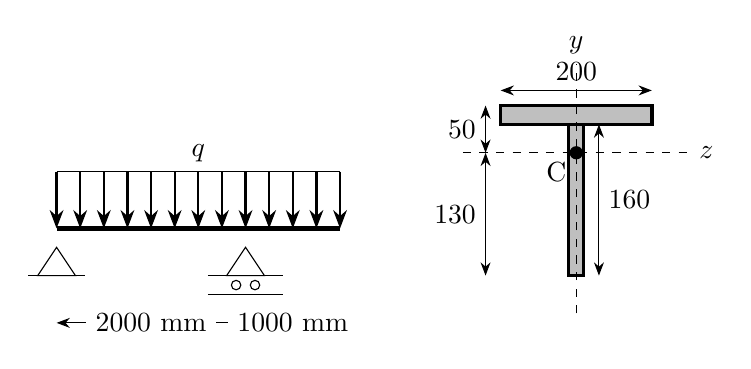
\begin{tikzpicture}[scale=1.2, >=Stealth]
% Beam axis and loads
\draw [line width=2.0pt] (0,0) -- (3,0);
\draw (0,-0.2) -- (0.2,-0.5) -- (-0.2,-0.5) -- cycle;
\draw (-0.3,-0.5) -- (0.3,-0.5);

\draw (2,-0.2) -- (2.2,-0.5) -- (1.8,-0.5) -- cycle;
\draw (1.6,-0.5) -- (2.4,-0.5);
\draw [fill=white] (1.9,-0.6) circle (0.05);
\draw [fill=white] (2.1,-0.6) circle (0.05);
\draw (1.6,-0.7) -- (2.4,-0.7);

\foreach \x in {0,0.25,0.5,0.75,1.0,1.25,1.5,1.75,2.0,2.25,2.5,2.75,3.0}
    \draw [->, line width=0.8pt] (\x, 0.6) -- (\x, 0);
\draw (0,0.6) -- (3,0.6);
\node [above] at (1.5,0.6) {$q$};

\draw [<->] (0,-1) -- (2,-1) node[midway, fill=white] {$2000\text{ mm}$};
\draw [<->] (2,-1) -- (3,-1) node[midway, fill=white] {$1000\text{ mm}$};

% T-section on the right
\begin{scope}[xshift=5.5cm, yshift=-0.5cm, scale=0.8]
    \draw [line width=1.2pt, fill=lightgray] (-1, 2.0) rectangle (1, 2.25);
    \draw [line width=1.2pt, fill=lightgray] (-0.1, 0) rectangle (0.1, 2.0);
    \draw [dashed] (-1.5, 1.625) -- (1.5, 1.625) node[right] {$z$};
    \draw [dashed] (0, -0.5) -- (0, 2.8) node[above] {$y$};
    \draw [fill=black] (0, 1.625) circle (0.08);
    \node [below left] at (0, 1.625) {C};
    
    \draw [<->] (-1.2, 0) -- (-1.2, 1.625) node[midway, left] {$130$};
    \draw [<->] (-1.2, 1.625) -- (-1.2, 2.25) node[midway, left] {$50$};
    \draw [<->] (-1, 2.45) -- (1, 2.45) node[midway, above] {$200$};
    \draw [<->] (0.3, 0) -- (0.3, 2.0) node[midway, right] {$160$};
\end{scope}
\end{tikzpicture}
\end{center}

\subsubsection*{解答：}

\textbf{1. 梁的内力分析}
均布荷载 $q=20\text{ kN/m}$ 作用于梁的全长 $AC=3\text{ m}$，其中 $AB=2\text{ m}$、外伸段 $BC=1\text{ m}$。设左支座为 A，右支座为 B，则
\[
R_A+R_B=q\cdot 3=60\text{ kN},\qquad
\sum M_A=0:\ R_B\cdot2-q\cdot3\cdot1.5=0.
\]
故
\[
R_A=15\text{ kN},\qquad R_B=45\text{ kN}.
\]
在 $AB$ 段内，取 $x$ 自 A 向 B：
\[
V_1(x)=15-20x,\qquad
M_1(x)=15x-10x^2\quad(0\le x\le2),
\]
在外伸段 $BC$ 内：
\[
V_2(x)=60-20x,\qquad
M_2(x)=60x-90-10x^2\quad(2\le x\le3),
\]
其中力单位为 kN、长度单位为 m。令 $V_1=0$ 得正弯矩最大截面
\[
x=0.75\text{ m},\qquad M_{\max}^{+}=5.625\text{ kN}\cdot\text{m}.
\]
B 支座截面处有最大负弯矩
\[
M_B=M_1(2)=M_2(2)=-10\text{ kN}\cdot\text{m}.
\]

\textbf{2. 弯曲正应力计算与校核}
已知形心 $C$ 距离截面底边 $y_{\text{bottom}}=130\text{ mm}$，距离截面顶边 $y_{\text{top}}=50\text{ mm}$，惯性矩 $I_z=2.136\times10^7\text{ mm}^4$。
正弯矩最大截面使下边缘受拉、上边缘受压。下边缘最大拉应力为
\[
\sigma_{t,+}=\frac{M_{\max}^{+}y_{\text{bottom}}}{I_z}
=\frac{5.625\times10^6\times130}{2.136\times10^7}
\approx34.23\text{ MPa}<[\sigma]^+=35\text{ MPa}.
\]
B 截面负弯矩使上边缘受拉、下边缘受压。上边缘拉应力为
\[
\sigma_{t,B}=\frac{|M_B|y_{\text{top}}}{I_z}
=\frac{10\times10^6\times50}{2.136\times10^7}
\approx23.41\text{ MPa}<[\sigma]^+=35\text{ MPa},
\]
下边缘压应力为
\[
\sigma_{c,B}=\frac{|M_B|y_{\text{bottom}}}{I_z}
=\frac{10\times10^6\times130}{2.136\times10^7}
\approx60.86\text{ MPa}>[\sigma]^-=60\text{ MPa}.
\]
\textbf{结论}：B 支座截面下边缘压应力略超过铸铁抗压许用应力，故该梁\textbf{不安全}。


% \newpage removed


\section*{3. 平面刚架位移计算}

\textbf{平面刚架受力如图所示，其中横杆和竖杆的弯曲刚度 $EI$、载荷集度 $q$、长度 $l$ 等均为已知。若忽略轴力和剪力的影响，试用卡氏第二定理（或莫尔积分法）求竖杆 AB 的中点 D 的水平位移。(25 分)}

\begin{center}
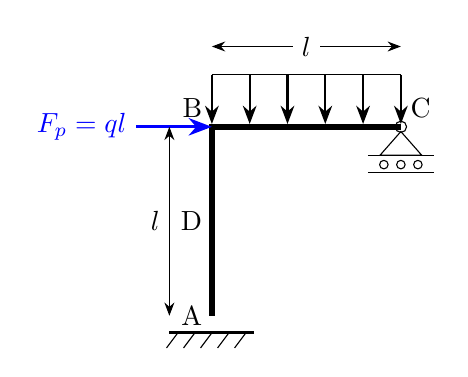
\begin{tikzpicture}[scale=1.2, >=Stealth]
\draw[line width=2.0pt] (0,0) coordinate(A) -- (0,2) coordinate(B) -- (2,2) coordinate(C);

% pin support at A
\draw[line width=1.2pt] (-0.45,-0.18) -- (0.45,-0.18);
\foreach \x in {-0.36,-0.18,0,0.18,0.36}
  \draw (\x,-0.18) -- (\x-0.12,-0.34);

% roller support at C
\draw (C) circle (0.06);
\draw (2,1.95) -- (2.22,1.70) -- (1.78,1.70) -- cycle;
\draw (1.65,1.70) -- (2.35,1.70);
\foreach \x in {1.82,2.0,2.18}
  \draw[fill=white] (\x,1.60) circle (0.045);
\draw (1.65,1.52) -- (2.35,1.52);

\node[left] at (A) {A};
\node[above left] at (B) {B};
\node[above right] at (C) {C};
\node[left] at (0,1) {D};

\draw[->, line width=1.2pt, blue] (-0.8,2.0) -- (0,2.0);
\node[left, blue] at (-0.8,2.0) {$F_p=ql$};

\foreach \x in {0,0.4,0.8,1.2,1.6,2.0}
  \draw[->, thick] (\x,2.55) -- (\x,2.03);
\draw (0,2.55) -- (2,2.55);
\node[above] at (1,2.55) {$q$};

\draw[<->] (-0.45,0) -- (-0.45,2) node[midway, left] {$l$};
\draw[<->] (0,2.85) -- (2,2.85) node[midway, fill=white] {$l$};
\end{tikzpicture}
\end{center}

\subsubsection*{解答：}

题图中 A 端固支，C 点为竖向滚支，结构为一次超静定刚架。取 C 点竖向反力 $R_C$ 为多余未知力，规定向上为正；竖杆 AB 取坐标 $y$ 自 A 向 B，横杆 BC 取坐标 $x$ 自 B 向 C。

\textbf{1. 由变形协调求 $R_C$}

撤去 C 点竖向支承，得到 A 端固支的基本结构。实际载荷作用下的弯矩为
\[
M_{AB}(y)=ql(l-y)+R_C l-\frac12ql^2\qquad(0\le y\le l),
\]
\[
M_{BC}(x)=R_C(l-x)-\frac12q(l-x)^2\qquad(0\le x\le l).
\]
C 点竖向位移为零，由卡氏第二定理得
\[
\frac{\partial U}{\partial R_C}
=\frac1{EI}\left[
\int_0^l M_{AB}l\diff y+\int_0^l M_{BC}(l-x)\diff x
\right]=0.
\]
代入上式：
\[
\int_0^l\left[ql(l-y)+R_C l-\frac12ql^2\right]l\diff y
+\int_0^l\left[R_C(l-x)-\frac12q(l-x)^2\right](l-x)\diff x=0,
\]
故
\[
R_C=\frac{3}{32}ql.
\]

\textbf{2. D 点单位水平力体系}

在 D 点沿所求位移正方向施加水平向右单位力。单位体系中 C 点竖向反力增量记为 $r_C$，对应单位弯矩为
\[
m_{AB}(y)=
\begin{cases}
\dfrac l2-y+r_C l, & 0\le y\le \dfrac l2,\\[4pt]
r_C l, & \dfrac l2\le y\le l,
\end{cases}
\qquad
m_{BC}(x)=r_C(l-x).
\]
同样由 C 点竖向位移协调：
\[
\int_0^l m_{AB}\,l\diff y+\int_0^l m_{BC}(l-x)\diff x=0,
\]
解得
\[
r_C=-\frac{3}{32}.
\]

\textbf{3. D 点水平位移}

将 $R_C=3ql/32$ 代回实际弯矩，作莫尔积分：
\[
\begin{aligned}
u_D
&=\frac1{EI}\left[
\int_0^l M_{AB}m_{AB}\diff y+\int_0^l M_{BC}m_{BC}\diff x
\right]\\
&=\frac1{EI}\left[
\frac{137}{3072}ql^4+\frac{9}{1024}ql^4
\right]
=\frac{41ql^4}{768EI}.
\end{aligned}
\]
单位力取向右，结果为正，故
\[
u_D=\frac{41ql^4}{768EI}\quad(\text{向右}).
\]


% \newpage removed


\section*{4. 结构安全最大载荷计算}

\textbf{图示梁 AB 在 A 端固支、在 C 点与杆 CD 铰接、在 B 点作用集中力 P。设梁 AB 和杆 CD 的横截面均为边长为 $b = a/10$ 的正方形，并且它们具有相同的弹性模量 $E$ 和许用应力 $[\sigma] = 0.5 \times 10^{-3} E$。杆 CD 的稳定安全因数 $[n]_{st} = 1.5$。若忽略剪力影响，试求保证结构安全的最大载荷 P。(25 分)}

\begin{center}
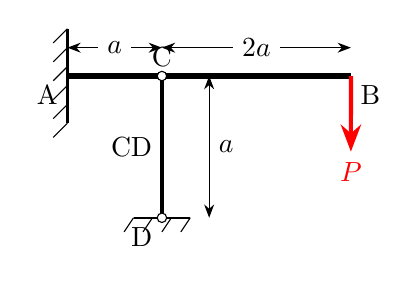
\begin{tikzpicture}[scale=1.2, >=Stealth]
% Wall at A
\draw[thick] (0,-0.5) -- (0,0.5);
\foreach \y in {-0.5,-0.3,-0.1,0.1,0.3,0.5}
  \draw (0,\y) -- (-0.15,\y-0.15);

% Beam AB
\draw[line width=2.0pt] (0,0) coordinate(A) -- (3,0) coordinate(B);

% Rod CD
\draw[line width=1.5pt] (1,0) coordinate(C) -- (1,-1.5) coordinate(D);
\draw[fill=white] (C) circle (0.05);

% Wall at D
\draw[thick] (0.7,-1.5) -- (1.3,-1.5);
\foreach \x in {0.7,0.9,1.1,1.3}
  \draw (\x,-1.5) -- (\x-0.1,-1.65);
\draw[fill=white] (D) circle (0.05);

% Force P
\draw[->, line width=1.5pt, red] (B) -- (3,-0.8) node[below] {$P$};

% Labels
\node[below left] at (A) {A};
\node[above] at (C) {C};
\node[below right] at (B) {B};
\node[left] at (1,-0.75) {CD};
\node[below left] at (D) {D};

% Dimensions
\draw[<->] (0,0.3) -- (1,0.3) node[midway, fill=white] {$a$};
\draw[<->] (1,0.3) -- (3,0.3) node[midway, fill=white] {$2a$};
\draw[<->] (1.5,0) -- (1.5,-1.5) node[midway, right] {$a$};
\end{tikzpicture}
\end{center}

\subsubsection*{解答：}

设杆 CD 顶端对梁 AB 施加的向上支撑力为 $R_C$。杆 CD 本身为两端铰支的受压杆件。

\textbf{1. 求解变形协调关系}
由梁 AB 在 C 点的向下挠度与杆 CD 的轴向压缩量相等：
\begin{itemize}
    \item 集中力 $P$ 引起的 C 点挠度：
    \[
    w_P = \frac{Pa^2}{6EI}(3 \times 3a - a) = \frac{4Pa^3}{3EI}
    \]
    \item 支撑力 $R_C$ 引起的 C 点挠度：
    \[
    w_R = -\frac{R_C a^3}{3EI}
    \]
    \item 杆 CD 自身的弹性压缩量为：
    \[
    \Delta l = \frac{R_C a}{EA_{\text{rod}}} = \frac{R_C a}{E b^2}
    \]
\end{itemize}
由变形协调 $w_P + w_R = \Delta l$ 得：
\[
\frac{4Pa^3}{3EI} - \frac{R_C a^3}{3EI} = \frac{R_C a}{E b^2}
\]
代入截面惯性矩 $I = \frac{b^4}{12}$ 和截面尺寸 $b = a/10$：
\[
\frac{160000 P}{E a} - \frac{40000 R_C}{E a} = \frac{100 R_C}{E a} \implies R_C = \frac{1600}{401}P \approx 3.99 P
\]

\textbf{2. 考虑结构各构件的承载限制条件}
\begin{itemize}
    \item \textbf{限制条件一：梁 AB 的弯曲强度} \\
    梁 AB 的弯矩图在 C 处取最大值 $M_C = 2Pa$。要求：
    \[
    \sigma_{\max} = \frac{M_C}{W} = \frac{2Pa}{\frac{1}{6}b^3} \le [\sigma] \implies \frac{12Pa}{\frac{a^3}{1000}} \le 0.5 \times 10^{-3} E \implies P \le 4.17 \times 10^{-8} Ea^2
    \]
    \item \textbf{限制条件二：杆 CD 的压缩强度} \\
    \[
    \sigma_{CD} = \frac{R_C}{b^2} \le [\sigma] \implies \frac{3.99 P}{\frac{a^2}{100}} \le 0.5 \times 10^{-3} E \implies P \le 1.25 \times 10^{-6} Ea^2
    \]
    \item \textbf{限制条件三：压杆 CD 的稳定安全性} \\
    压杆 CD 两端铰支 ($\mu = 1.0$)，临界载荷由欧拉公式给出：
    \[
    P_{cr} = \frac{\pi^2 EI_{CD}}{a^2} = \frac{\pi^2 E b^4}{12 a^2} = \frac{\pi^2 E a^2}{120000}
    \]
    稳定许用荷载为 $[P]_{st} = \frac{P_{cr}}{[n]_{st}} = \frac{\pi^2 E a^2}{180000}$。要求：
    \[
    R_C \le [P]_{st} \implies 3.99 P \le \frac{\pi^2 E a^2}{180000} \implies P \le 1.37 \times 10^{-5} Ea^2
    \]
\end{itemize}

比较上述三个限制条件，取最小值作为保证结构安全的最大载荷：
\[
P_{\max} = 4.17 \times 10^{-8} Ea^2
\]


}

\chapter{材料力学 2007 年期末测验试题 (A) 修订解答}
{

\renewcommand{\assetdir}{../../考题_按知识点整理/visual_assets/question_crops/2007_2007年期末_A卷}

\section*{一、悬臂梁变形及超静定分析 (25 分)}

\begin{center}
    \includegraphics[width=0.8\textwidth]{\assetdir/q-001.png}
\end{center}

\textbf{悬臂梁如图(a)，A 端固定支撑，B 端自由，梁上作用有垂直向上的函数分布载荷，若梁的挠度以向上为正，A 端的载荷分布值为 $q_0$，挠度表达式为：}
\[
w(x) = \frac{q_0 L^4}{360 EI} \left[ 45\left(\frac{x}{L}\right)^2 - 40\left(\frac{x}{L}\right)^3 + 15\left(\frac{x}{L}\right)^4 - \left(\frac{x}{L}\right)^6 \right]
\]
\textbf{试求：}
\textbf{(1) 梁上截面转角的函数表达式；}
\textbf{(2) 梁上截面弯矩的函数表达式；}
\textbf{(3) 梁上截面剪力的函数表达式；}
\textbf{(4) 梁上的载荷分布函数；}
\textbf{(5) 梁上固定端 A 截面的约束力和约束力偶；}
\textbf{(6) 如果在 AB 梁的中点 C 处增加一个滚轴约束（如图（b）），求此滚轴的约束力的方向和大小。}

\subsubsection*{解答：}

以梁的最左端为原点 $O$（即 A 点），以梁的轴线为 $x$ 轴。设挠度 $w(x)$ 向上为正，转角 $\theta(x) = \frac{\diff w}{\diff x}$ 逆时针为正。

\textbf{(1) 截面转角函数 $\theta(x)$}
对挠度 $w(x)$ 求一阶导数：
\[
\theta(x) = \frac{\diff w}{\diff x} = \frac{q_0 L^4}{360 EI} \left[ \frac{90x}{L^2} - \frac{120x^2}{L^3} + \frac{60x^3}{L^4} - \frac{6x^5}{L^6} \right] = \frac{q_0 x}{60 EI L^2} \left( 15L^4 - 20L^3 x + 10L^2 x^2 - x^4 \right)
\]

\textbf{(2) 截面弯矩函数 $M(x)$}
由于挠度以向上为正，其微分方程关系为 $EI \frac{\diff^2 w}{\diff x^2} = M(x)$。
对 $w(x)$ 求二阶导数：
\[
M(x) = EI \frac{\diff^2 w}{\diff x^2} = \frac{q_0 L^4}{360} \left[ \frac{90}{L^2} - \frac{240x}{L^3} + \frac{180x^2}{L^4} - \frac{30x^4}{L^6} \right] = \frac{q_0}{12 L^2} \left( 3L^4 - 8L^3 x + 6L^2 x^2 - x^4 \right)
\]

\textbf{(3) 截面剪力函数 $Q(x)$}
剪力与弯矩的关系为 $Q(x) = \frac{\diff M}{\diff x}$：
\[
Q(x) = \frac{\diff M}{\diff x} = \frac{q_0}{12 L^2} \left( -8L^3 + 12L^2 x - 4x^3 \right) = q_0 \left( -\frac{2}{3}L + x - \frac{x^3}{3L^2} \right)
\]

\textbf{(4) 载荷分布函数 $q(x)$}
载荷集度与剪力的关系为 $q(x) = \frac{\diff Q}{\diff x}$：
\[
q(x) = \frac{\diff Q}{\diff x} = q_0 \left( 1 - \frac{x^2}{L^2} \right)
\]
方向向上。当 $x=0$ 时 $q(0) = q_0$，当 $x=L$ 时 $q(L) = 0$。

\textbf{(5) 固定端 A 截面的约束力与约束力偶}
根据 A 点 ($x=0$) 处的内力：
\noindent\textbullet\ 剪力 $Q(0) = -\frac{2}{3}q_0 L$，故固定端向下的约束力为 $R_A = \frac{2}{3}q_0 L$。
\noindent\textbullet\ 弯矩 $M(0) = \frac{1}{4}q_0 L^2$，故固定端的约束力偶矩为 $M_A = \frac{1}{4}q_0 L^2$（顺时针，平衡向上载荷产生的逆时针力矩）。

\textbf{(6) 中点 C 处增加滚轴约束时的约束力}
设 C 点的滚轴约束力为 $R_C$（方向向下）。
\noindent\textbullet\ 在分布载荷 $q(x)$ 作用下，C 点 ($x=L/2$) 的向上挠度为：
  \[
  w_{C, q} = w\left(\frac{L}{2}\right) = \frac{q_0 L^4}{360 EI} \left[ 45\left(\frac{1}{2}\right)^2 - 40\left(\frac{1}{2}\right)^3 + 15\left(\frac{1}{2}\right)^4 - \left(\frac{1}{2}\right)^6 \right] = \frac{51 q_0 L^4}{2560 EI}
  \]
\noindent\textbullet\ 集中力 $R_C$ 作用于悬臂梁中点 C 时，引起的 C 点向下变形为：
  \[
  w_{C, R} = \frac{R_C (L/2)^3}{3EI} = \frac{R_C L^3}{24 EI}
  \]
\noindent\textbullet\ 根据变形协调条件 $w_{C, q} - w_{C, R} = 0$：
  \[
  \frac{51 q_0 L^4}{2560 EI} = \frac{R_C L^3}{24 EI} \implies R_C = \frac{153}{320} q_0 L \approx 0.478 q_0 L \quad (\text{方向向下})
  \]


% \newpage removed


\section*{二、管钳与受扭管件的强度校核 (25 分)}

\begin{center}
    \includegraphics[width=0.65\textwidth]{\assetdir/q-002.png}
\end{center}

\textbf{垂直向下的 $200\text{ N}$ 力作用在管钳的手柄上，手柄与 $z$ 轴平行。管子左端 $x=0$ 处视作固支，外径 $D=32\text{ mm}$，内径 $d=26\text{ mm}$。手柄作用力位置的 $z$ 坐标为 $0.2\text{ m}$，到固支端距离为 $0.3\text{ m}$（即 $x=0.3\text{ m}$）。试求：}
\textbf{(1) 通过 A 点和 B 点的截面（固支端截面 $x=0$）上的剪力、弯矩和扭矩；}
\textbf{(2) 用微元表示 A 点和 B 点的正应力和切应力的方向和大小（忽略剪力产生的切应力）；}
\textbf{(3) 给出 A 点和 B 点主应力的大小；}
\textbf{(4) 如果用最大切应力准则验证管子的强度，试给出管子上最大切应力的值。}

\subsubsection*{解答：}

\textbf{(1) 固支端截面上的内力计算}
力 $F = 200\text{ N}$ 沿 $-y$ 方向作用，其作用点坐标为 $x = 0.3\text{ m}$, $z = 0.2\text{ m}$。对固支端截面 $x=0$：
\noindent\textbullet\ 剪力：$V_y = F = 200\text{ N}$。
\noindent\textbullet\ 弯矩（关于 $z$ 轴）：$M_z = F \cdot x = 200 \times 0.3 = 60\text{ N}\cdot\text{m}$。
\noindent\textbullet\ 扭矩（关于 $x$ 轴）：$T_x = F \cdot z = 200 \times 0.2 = 40\text{ N}\cdot\text{m}$。

\textbf{(2) A 点和 B 点的应力状态}
管子的截面几何性质：
\[
I_z = \frac{\pi}{64} (D^4 - d^4) = \frac{\pi}{64} (32^4 - 26^4) \approx 29040\text{ mm}^4 = 2.904 \times 10^{-8}\text{ m}^4
\]
\[
I_p = 2 I_z \approx 5.808 \times 10^{-8}\text{ m}^4
\]
\noindent\textbullet\ \textbf{A 点（最上端 $y = R = 16\text{ mm}$）}：
\noindent\textbullet\ 正应力由弯矩产生（受拉）：
    \[
    \sigma_x = \frac{M_z R}{I_z} = \frac{60 \times 0.016}{2.904 \times 10^{-8}} \approx 33.06\text{ MPa}
    \]
\noindent\textbullet\ 切应力由扭矩产生：
    \[
    \tau_x = \frac{T_x R}{I_p} = \frac{40 \times 0.016}{5.808 \times 10^{-8}} \approx 11.02\text{ MPa}
    \]
\noindent\textbullet\ \textbf{B 点（侧面中性轴上 $y = 0, z = R = 16\text{ mm}$）}：
\noindent\textbullet\ 正应力为 0（位于弯曲中性轴上）：$\sigma_x = 0$。
\noindent\textbullet\ 切应力由扭矩产生：
    \[
    \tau_x = \frac{T_x R}{I_p} \approx 11.02\text{ MPa}
    \]
微元表示时，A 点画轴向拉应力 $\sigma_x$ 和由扭矩 $T_x$ 产生的切应力 $\tau_x$；B 点位于弯曲中性轴，只画扭转剪应力。剪应力箭头按右手螺旋方向与题图扭矩 $T_x$ 保持一致。

\textbf{(3) A 点和 B 点的主应力}
\noindent\textbullet\ \textbf{A 点}的应力状态为 $\sigma_x = 33.06\text{ MPa}$，$\tau_{xy} = 11.02\text{ MPa}$：
  \[
  \sigma_{1,3} = \frac{\sigma_x}{2} \pm \sqrt{\left(\frac{\sigma_x}{2}\right)^2 + \tau_x^2} = 16.53 \pm \sqrt{16.53^2 + 11.02^2} = 16.53 \pm 19.87\text{ MPa}
  \]
  解得：$\sigma_1 = 36.39\text{ MPa}$，$\sigma_2 = 0$，$\sigma_3 = -3.34\text{ MPa}$。
\noindent\textbullet\ \textbf{B 点}的应力状态为纯剪切 $\tau = 11.02\text{ MPa}$：
  解得：$\sigma_1 = 11.02\text{ MPa}$，$\sigma_2 = 0$，$\sigma_3 = -11.02\text{ MPa}$。

\textbf{(4) 管子上的最大切应力}
管子上弯矩和扭矩最大的截面均为固支端 $x=0$，且在管子的最外层表面（A 点及其对称点）。
最大切应力值为：
\[
\tau_{\max} = \frac{\sigma_1 - \sigma_3}{2} = \sqrt{\left(\frac{\sigma_x}{2}\right)^2 + \tau_x^2} \approx 19.87\text{ MPa}
\]


% \newpage removed


\section*{三、压杆稳定与温度应力分析 (20 分)}

\begin{center}
    \includegraphics[width=0.55\textwidth]{\assetdir/q-003.png}
\end{center}

\textbf{直径为 $d$，长为 $L$ 的圆截面直杆，两端在初始温度固定时，任意截面为无应力状态。(a) 为两端铰支，(b) 为一端固支，一端铰支。当温度升高后，若假设杆件的失稳为弹性失稳，试求：}
\textbf{(1) 杆件的内力和截面上的正应力与温度变化量 $\Delta T$ 之间的关系；}
\textbf{(2) 两种约束情况下杆件各自能够承受的临界失稳温度升高值 $\Delta T_{cr}$；}
\textbf{(3) 两种约束情况下的临界载荷比。}

\subsubsection*{解答：}

\textbf{(1) 内力与正应力与温度变化量 $\Delta T$ 的关系}
两端固定约束限制了直杆的轴向变形。自由温度升高 $\Delta T$ 时产生的热应变为 $\epsilon_{th} = \alpha \Delta T$。由于总变形为零：
\[
\epsilon = \frac{\sigma}{E} + \alpha \Delta T = 0 \implies \sigma = -E \alpha \Delta T \quad (\text{受压应力})
\]
杆件的压轴力大小为：
\[
P = |\sigma| A = E \alpha \Delta T \frac{\pi d^2}{4}
\]

\textbf{(2) 临界失稳温度升高值 $\Delta T_{cr}$}
根据欧拉公式，临界压应力为：
\[
\sigma_{cr} = \frac{\pi^2 E}{\lambda^2} = \frac{\pi^2 E I}{\mu^2 L^2 A}
\]
其中圆截面的惯性矩 $I = \frac{\pi d^4}{64}$，面积 $A = \frac{\pi d^2}{4}$，故 $\frac{I}{A} = \frac{d^2}{16}$。
令 $\sigma = \sigma_{cr}$，即 $E \alpha \Delta T_{cr} = \frac{\pi^2 E d^2}{16 \mu^2 L^2}$：
\[
\Delta T_{cr} = \frac{\pi^2 d^2}{16 \mu^2 \alpha L^2}
\]
\noindent\textbullet\ \textbf{(a) 两端铰支} ($\mu = 1.0$)：
  \[
  \Delta T_{cr, a} = \frac{\pi^2 d^2}{16 \alpha L^2}
  \]
\noindent\textbullet\ \textbf{(b) 一端固支，一端铰支} ($\mu = 0.7$)：
  \[
  \Delta T_{cr, b} = \frac{\pi^2 d^2}{16 \times 0.7^2 \alpha L^2} = \frac{\pi^2 d^2}{7.84 \alpha L^2} \approx 2.04 \Delta T_{cr, a}
  \]

\textbf{(3) 两种约束情况下的临界载荷比}
临界载荷与长度系数平方成反比：
\[
P_{cr, a} : P_{cr, b} = \frac{1}{\mu_a^2} : \frac{1}{\mu_b^2} = \frac{1}{1.0^2} : \frac{1}{0.7^2} = 0.49 : 1
\]


% \newpage removed


\section*{四、梁的变形计算与叠加原理 (25 分)}

\begin{center}
    \includegraphics[width=0.6\textwidth]{\assetdir/q-004.png}
\end{center}

\textbf{(1) 用叠加原理给出 (a) 和 (b) 的挠度表达式；}
\textbf{(2) 计算 (b) 杆件的最大挠度值及其位置。}
\textbf{其中设杆件的弹性模量为 $E$，截面为矩形，惯性矩为 $I$。}

\subsubsection*{解答：}

\textbf{(1) 挠度表达式 (a)}
图(a)为简支梁，跨度为 $L$，承受从 $q_0$ 到 $2q_0$ 的渐变（梯形）载荷，向下。
该载荷可分解为两部分：
1. 均布载荷 $q_1 = q_0$。
2. 三角形分布载荷 $q_2(x) = q_0 \frac{x}{L}$（$x=0$ 处为 $0$，$x=L$ 处为 $q_0$）。
两部分对应的挠度公式分别为：
\noindent\textbullet\ 均布载荷 $q_0$ 产生的挠度：
  \[
  w_1(x) = \frac{q_0 x}{24EI} (L^3 - 2Lx^2 + x^3)
  \]
\noindent\textbullet\ 三角形载荷 $q_0 \frac{x}{L}$ 产生的挠度：
  \[
  w_2(x) = \frac{q_0 x}{360 EIL} (7L^4 - 10L^2 x^2 + 3x^4)
  \]
叠加后，简支梁的向下挠度表达式为：
\[
w_a(x) = w_1(x) + w_2(x) = \frac{q_0 x (L - x)}{360 EI L} \left( 22 L^3 + 22 L^2 x - 18 L x^2 - 3 x^3 \right)
\]

\textbf{(2) 挠度表达式及最大挠度 (b)}
图(b)为悬臂梁，固定端在 $x=0$，自由端在 $x=L$。载荷为：$0\le x\le L/2$ 段为均布载荷 $q_0$，$L/2\le x\le L$ 段从 $q_0$ 线性减小到 0。

求自由端最大挠度时，在自由端沿载荷方向（向下）加单位力，虚拟弯矩为 $m(x)=L-x$。实际弯矩为
\[
M(x)=\frac{q_0}{24}\left(7L^2-18Lx+12x^2\right)\quad(0\le x\le L/2)
\]
\[
M(x)=\frac{q_0}{3L}(L-x)^3\quad(L/2\le x\le L)
\]
因此自由端挠度为
\[
w_b(L)=\frac{1}{EI}\left[
\int_0^{L/2}\frac{q_0}{24}\left(7L^2-18Lx+12x^2\right)(L-x)\diff x
+\int_{L/2}^{L}\frac{q_0}{3L}(L-x)^4\diff x
\right]
=\frac{119q_0L^4}{1920EI}
\]
最大挠度发生在自由端 $x=L$，方向与载荷方向相同。


% \newpage removed


\section*{五、双层薄壁圆环温差缩紧应力分析 (5 分)}

\begin{center}
    \includegraphics[width=0.45\textwidth]{\assetdir/q-005.png}
\end{center}

\textbf{两个薄壁圆环（材料相同，弹性模量为 $E$）紧密套在一起。在没有套在一起的初始温度下，外环内直径为 $D_1$，壁厚为 $\delta_1$；内环内直径为 $D_2$，壁厚为 $\delta_2$；内环外直径比外环内直径大 $\zeta$。求冷却到初始温度后，两环间的均匀接触压力 $p$ 以及两环的环向应力 $\sigma_{\theta1}$、$\sigma_{\theta2}$。}

\subsubsection*{解答：}

记外环内、外半径为
\[
a_1=\frac{D_1}{2},\qquad b_1=a_1+\delta_1,
\]
内环内、外半径为
\[
a_2=\frac{D_2}{2},\qquad b_2=a_2+\delta_2.
\]
题给过盈量为外环内直径与内环外直径之差，所以半径方向的过盈为
\[
b_2-a_1=\frac{\zeta}{2}.
\]

轴对称圆环在内压 $p_i$、外压 $p_o$ 作用下有
\[
\sigma_r=A-\frac{B}{r^2},\qquad
\sigma_\theta=A+\frac{B}{r^2},
\]
\[
A=\frac{p_i a^2-p_o b^2}{b^2-a^2},\qquad
B=\frac{a^2b^2(p_i-p_o)}{b^2-a^2},
\]
由题给的应变关系和 $\varepsilon_r=\diff u/\diff r,\ \varepsilon_\theta=u/r$ 可得位移
\[
u(r)=\frac{1}{E}\left[(1-\nu)Ar+(1+\nu)\frac{B}{r}\right].
\]

外环受内压 $p$，即 $p_i=p,\ p_o=0$，其内表面向外胀大量为
\[
u_1=u_o(a_1)
=\frac{p a_1}{E(b_1^2-a_1^2)}
\left[(1-\nu)a_1^2+(1+\nu)b_1^2\right].
\]
内环受外压 $p$，即 $p_i=0,\ p_o=p$，其外表面向内缩小量为
\[
u_2=-u_i(b_2)
=\frac{p b_2}{E(b_2^2-a_2^2)}
\left[(1-\nu)b_2^2+(1+\nu)a_2^2\right].
\]
变形协调条件为
\[
u_1+u_2=\frac{\zeta}{2}.
\]
故两环间均匀接触压力为
\[
p=
\frac{E\zeta/2}
{\dfrac{a_1\left[(1-\nu)a_1^2+(1+\nu)b_1^2\right]}{b_1^2-a_1^2}
+\dfrac{b_2\left[(1-\nu)b_2^2+(1+\nu)a_2^2\right]}{b_2^2-a_2^2}}.
\]

两环中的环向应力分布分别为
\[
\sigma_{\theta1}(r)=
\frac{p a_1^2}{b_1^2-a_1^2}
\left(1+\frac{b_1^2}{r^2}\right)
\quad (a_1\le r\le b_1),
\]
\[
\sigma_{\theta2}(r)=
-\frac{p b_2^2}{b_2^2-a_2^2}
\left(1+\frac{a_2^2}{r^2}\right)
\quad (a_2\le r\le b_2).
\]
其中外环为环向拉应力，内环为环向压应力。

若按题意进一步采用薄壁近似，令界面直径近似为 $D$，则
\[
p=\frac{2E\zeta}{D^2\left(\dfrac1{\delta_1}+\dfrac1{\delta_2}\right)}
=\frac{2E\zeta\delta_1\delta_2}{D^2(\delta_1+\delta_2)},
\]
\[
\sigma_{\theta1}\simeq \frac{pD}{2\delta_1}
=\frac{E\zeta\delta_2}{D(\delta_1+\delta_2)},\qquad
\sigma_{\theta2}\simeq -\frac{pD}{2\delta_2}
=-\frac{E\zeta\delta_1}{D(\delta_1+\delta_2)}.
\]


}

\chapter{材料力学 2007 年期末测验试题 (B) 修订解答}
{



\section*{1. 连续梁的变形计算与约束反力 (20 分)}

\textbf{如图所示，已知 $q$、$EI$、$l$。试根据梁的挠曲线微分方程和约束条件，求梁的挠度曲线表达式，并给出截面 A 的挠度和截面 B 的转角。}

\subsubsection*{解答：}

以最左端支座为原点 $O$，以梁的轴心线为 $x$ 轴，向上为挠度 $w(x)$ 的正方向。梁分为两个部分：
\noindent\textbullet\ 第一段 $OB$（$0 \le x \le 2l$）：受 $x=l$ 处的集中力 $P = ql$（向下）。
\noindent\textbullet\ 第二段 $BA$（$2l \le x \le 3l$）：受均布载荷 $q$（向下）。

根据静定关系，可求得支座反力：
设左支座 $O$ 处向上反力为 $R_O$，中间支座 $B$ ($x=2l$) 处向上反力为 $R_B$。
\noindent\textbullet\ 对整个梁列矩平衡方程（绕 $B$ 点）：
  \[
  R_O \cdot 2l - (ql) \cdot l + q \cdot l \cdot \frac{l}{2} = 0 \implies 2 R_O l - q l^2 + \frac{1}{2} q l^2 = 0 \implies R_O = \frac{1}{4} ql \quad (\text{向上})
  \]
\noindent\textbullet\ 竖向受力平衡：
  \[
  R_O + R_B = ql + ql = 2ql \implies R_B = 2ql - \frac{1}{4}ql = \frac{7}{4} ql \quad (\text{向上})
  \]

\textbf{1. 弯矩方程 $M(x)$ 与挠曲线微分方程}
\noindent\textbullet\ 在 $0 \le x < l$ 段：
  \[
  EI w_1''(x) = M_1(x) = R_O x = \frac{1}{4} ql x
  \]
\noindent\textbullet\ 在 $l \le x < 2l$ 段：
  \[
  EI w_2''(x) = M_2(x) = R_O x - ql(x-l) = -\frac{3}{4} ql x + ql^2
  \]
\noindent\textbullet\ 在 $2l \le x \le 3l$ 段（也可以从自由端 $A$ 开始列式，设离 $A$ 的距离为 $t = 3l - x$）：
  \[
  EI w_3''(x) = M_3(x) = -\frac{1}{2} q (3l-x)^2 = -\frac{1}{2} q (9l^2 - 6lx + x^2)
  \]

\textbf{2. 积分求解挠度曲线}
\noindent\textbullet\ \textbf{第一段 $0 \le x < l$}：
  \[
  EI w_1'(x) = \frac{1}{8} ql x^2 + C_1
  \]
  \[
  EI w_1(x) = \frac{1}{24} ql x^3 + C_1 x + D_1
  \]
  由于 $x=0$ 处 $w_1(0) = 0$，得 $D_1 = 0$。
\noindent\textbullet\ \textbf{第二段 $l \le x < 2l$}：
  \[
  EI w_2'(x) = -\frac{3}{8} ql x^2 + ql^2 x + C_2
  \]
  \[
  EI w_2(x) = -\frac{1}{8} ql x^3 + \frac{1}{2} ql^2 x^2 + C_2 x + D_2
  \]
\noindent\textbullet\ \textbf{第三段 $2l \le x \le 3l$}：
  \[
  EI w_3'(x) = \frac{1}{6} q (3l-x)^3 + C_3
  \]
  \[
  EI w_3(x) = -\frac{1}{24} q (3l-x)^4 + C_3 x + D_3
  \]

\textbf{3. 边界条件与连续性条件}
1. 在 $x=l$ 处的连续性条件（$w_1(l) = w_2(l)$, $w_1'(l) = w_2'(l)$）：
   \[
   \frac{1}{8} ql^3 + C_1 = -\frac{3}{8} ql^3 + ql^3 + C_2 \implies C_1 - C_2 = \frac{1}{2} ql^3
   \]
   \[
   \frac{1}{24} ql^4 + C_1 l = -\frac{1}{8} ql^4 + \frac{1}{2} ql^4 + C_2 l + D_2 \implies (C_1 - C_2)l - D_2 = \frac{1}{3} ql^4 \implies D_2 = \frac{1}{6} ql^4
   \]
2. 支座 $B$ 处 ($x=2l$) 处的挠度为零（$w_2(2l) = 0$, $w_3(2l) = 0$）：
   \[
   -\frac{1}{8} ql (2l)^3 + \frac{1}{2} ql^2 (2l)^2 + C_2 (2l) + \frac{1}{6} ql^4 = 0 \implies -ql^4 + 2ql^4 + 2 C_2 l + \frac{1}{6} ql^4 = 0 \implies C_2 = -\frac{7}{12} ql^3
   \]
   解得 $C_1 = C_2 + \frac{1}{2} ql^3 = -\frac{1}{12} ql^3$。
   同时由 $w_3(2l) = 0$：
   \[
   -\frac{1}{24} q l^4 + C_3 (2l) + D_3 = 0 \implies 2 C_3 l + D_3 = \frac{1}{24} ql^4
   \]
3. 在 $x=2l$ 处的转角连续性条件（$w_2'(2l) = w_3'(2l)$）：
   \[
   EI w_2'(2l) = -\frac{3}{8} ql (2l)^2 + ql^2 (2l) + C_2 = -\frac{3}{2} ql^3 + 2ql^3 - \frac{7}{12} ql^3 = -\frac{1}{12} ql^3
   \]
   \[
   EI w_3'(2l) = \frac{1}{6} q (l)^3 + C_3 = \frac{1}{6} ql^3 + C_3
   \]
   两者相等：
   \[
   \frac{1}{6} ql^3 + C_3 = -\frac{1}{12} ql^3 \implies C_3 = -\frac{1}{4} ql^3
   \]
   进而求得 $D_3$：
   \[
   D_3 = \frac{1}{24} ql^4 - 2 C_3 l = \frac{1}{24} ql^4 + \frac{1}{2} ql^4 = \frac{13}{24} ql^4
   \]

各段挠度表达式为：
\noindent\textbullet\ $0 \le x < l$：$w_1(x) = \frac{ql}{24EI} x^3 - \frac{ql^3}{12EI} x$
\noindent\textbullet\ $l \le x < 2l$：$w_2(x) = -\frac{ql}{8EI} x^3 + \frac{ql^2}{2EI} x^2 - \frac{7ql^3}{12EI} x + \frac{ql^4}{6EI}$
\noindent\textbullet\ $2l \le x \le 3l$：$w_3(x) = -\frac{q}{24EI} (3l-x)^4 - \frac{ql^3}{4EI} x + \frac{13ql^4}{24EI}$

\textbf{A 点的挠度 $w_A$ ($x=3l$)}：
\[
w_A = w_3(3l) = -\frac{ql^3}{4EI} (3l) + \frac{13ql^4}{24EI} = -\frac{5}{24} \frac{q l^4}{EI} \quad (\text{方向向下})
\]

\textbf{B 点的转角 $\theta_B$ ($x=2l$)}：
\[
\theta_B = w_2'(2l) = -\frac{1}{12} \frac{q l^3}{EI} \quad (\text{顺时针})
\]


% \newpage removed


\section*{2. 带有间隙的超静定梁弯曲内力分析 (20 分)}

\textbf{梁的 A 端固支、B 端在加载前与支承之间有一间隙 $\delta_0$，在梁的中点施加力矩 $M$。设梁的弯曲刚度 $EI$ 已知，试作出梁的弯矩图和剪力图。}

\subsubsection*{解答：}

以 A 点为原点，设梁总长度为 $2L$，中点为 C（$x=L$），右端为 B（$x=2L$）。

\textbf{1. 间隙未闭合情况}
如果施加的弯矩较小，梁的右端变形 $w_B$ 未达到间隙 $\delta_0$，则 B 端约束不起作用，梁为静定悬臂梁。
\noindent\textbullet\ A 端固定端反力：$M_A = M$（顺时针），支反力为 0。
\noindent\textbullet\ 弯矩分布：
\noindent\textbullet\ $0 < x < L$（AC 段）：$M(x) = M$
\noindent\textbullet\ $L < x < 2L$（CB 段）：$M(x) = 0$
\noindent\textbullet\ 剪力分布：$Q(x) = 0$。
\noindent\textbullet\ B 点的挠度 $w_B$：
\noindent\textbullet\ C 点的转角为 $\theta_C = \frac{ML}{EI}$。
\noindent\textbullet\ C 点的挠度为 $w_C = \frac{ML^2}{2EI}$。
\noindent\textbullet\ 由于 CB 段无弯矩，为直线段：
    \[
    w_B = w_C + \theta_C \cdot L = \frac{ML^2}{2EI} + \frac{ML^2}{EI} = \frac{3ML^2}{2EI}
    \]
\noindent\textbullet\ 间隙刚好闭合的临界弯矩 $M_{cr}$：
  \[
  \frac{3 M_{cr} L^2}{2 EI} = \delta_0 \implies M_{cr} = \frac{2 EI \delta_0}{3 L^2}
  \]
  当 $M \le M_{cr}$ 时，剪力图为 0，弯矩图在 AC 段为矩形 $M$，CB 段为 0。

\textbf{2. 间隙闭合情况 ($M > M_{cr}$)}
当 $M > M_{cr}$ 时，B 端与支座接触，产生向上反力 $R_B$。
系统为一次超静定梁。根据变形协调条件，B 端的最终挠度为 $\delta_0$。
\noindent\textbullet\ 利用叠加原理，B 端的挠度为施加弯矩 $M$ 产生的挠度减去 $R_B$ 产生的挠度：
  \[
  w_B = \frac{3ML^2}{2EI} - \frac{R_B (2L)^3}{3EI} = \delta_0
  \]
  \[
  \frac{8 R_B L^3}{3 EI} = \frac{3ML^2}{2EI} - \delta_0 \implies R_B = \frac{9M}{16L} - \frac{3EI \delta_0}{8L^3}
  \]
\noindent\textbullet\ 剪力分布：
  \[
  Q(x) = -R_B = -\left( \frac{9M}{16L} - \frac{3EI \delta_0}{8L^3} \right) \quad (0 < x < 2L)
  \]
\noindent\textbullet\ 弯矩分布：
\noindent\textbullet\ $L < x \le 2L$（CB 段）：
    \[
    M(x) = -R_B (2L - x)
    \]
\noindent\textbullet\ $0 \le x < L$（AC 段）：
    \[
    M(x) = M - R_B (2L - x)
    \]

\textbf{3. 剪力图和弯矩图}

\begin{figure}[H]
\centering
\begin{tikzpicture}[x=2.0cm,y=0.72cm,>=Latex]
  \node[anchor=west] at (-0.15,2.25) {间隙未闭合：$M\le M_{cr}$};
  \draw[->] (-0.1,0) -- (2.25,0) node[right] {$x/L$};
  \draw[->] (0,-0.45) -- (0,1.15) node[above] {$Q$};
  \foreach \x/\lab in {0/A,1/C,2/B}{
    \draw[densely dashed,gray] (\x,-0.25)--(\x,0.95);
    \node[below] at (\x,-0.3) {$\lab$};
  }
  \draw[very thick,blue] (0,0)--(2,0);
  \node[above] at (1.2,0) {$Q=0$};

  \begin{scope}[yshift=-4.0cm]
    \draw[->] (-0.1,0) -- (2.25,0) node[right] {$x/L$};
    \draw[->] (0,-0.45) -- (0,1.35) node[above] {$M_b$};
    \foreach \x/\lab in {0/A,1/C,2/B}{
      \draw[densely dashed,gray] (\x,-0.25)--(\x,1.15);
      \node[below] at (\x,-0.3) {$\lab$};
    }
    \draw[very thick,red] (0,1)--(1,1);
    \draw[very thick,red] (1,1)--(1,0);
    \draw[very thick,red] (1,0)--(2,0);
    \node[left] at (0,1) {$M$};
    \node[above] at (1.5,0) {$0$};
  \end{scope}

  \begin{scope}[xshift=6.0cm]
    \node[anchor=west] at (-0.15,2.25) {间隙闭合：$M>M_{cr}$};
    \draw[->] (-0.1,0) -- (2.25,0) node[right] {$x/L$};
    \draw[->] (0,-1.15) -- (0,0.65) node[above] {$Q$};
    \foreach \x/\lab in {0/A,1/C,2/B}{
      \draw[densely dashed,gray] (\x,-0.95)--(\x,0.45);
      \node[below] at (\x,-1.0) {$\lab$};
    }
    \draw[very thick,blue] (0,-0.75)--(2,-0.75);
    \node[below] at (1,-0.75) {$-R_B$};

    \begin{scope}[yshift=-4.0cm]
      \draw[->] (-0.1,0) -- (2.25,0) node[right] {$x/L$};
      \draw[->] (0,-1.25) -- (0,1.45) node[above] {$M_b$};
      \foreach \x/\lab in {0/A,1/C,2/B}{
        \draw[densely dashed,gray] (\x,-1.05)--(\x,1.2);
        \node[below] at (\x,-1.1) {$\lab$};
      }
      \draw[very thick,red] (0,0.8)--(1,1.1);
      \draw[very thick,red] (1,1.1)--(1,-0.7);
      \draw[very thick,red] (1,-0.7)--(2,0);
      \node[left] at (0,0.8) {$M-2R_BL$};
      \node[above] at (1,1.1) {$M-R_BL$};
      \node[right] at (1,-0.7) {$-R_BL$};
      \node[above] at (2,0) {$0$};
    \end{scope}
  \end{scope}
\end{tikzpicture}
\caption{题 2 两种工况下的剪力图和弯矩图}
\end{figure}


% \newpage removed


\section*{3. 斜向力作用下的悬臂梁强度校核 (20 分)}

\textbf{矩形截面悬臂梁（200mm $\times$ 120mm $\times$ 1200mm）左端固定，右端中心施加面内沿 $\theta = 30^\circ$ 方向的集中力 $F_p = 100\text{ KN}$。已知材料的许用应力 $[\sigma]=30\text{ MPa}$。求：固定端截面上 A、B、C、D 四点的正应力，并在不考虑剪切应力影响的情况下判断梁的强度是否满足要求。}

\subsubsection*{解答：}

题中说力作用在端面内，因此 $F_p$ 不产生轴力，而应分解为截面内的 $y,z$ 两个横向分量。取 $y$ 向上，$z$ 沿图中 $200\text{ mm}$ 宽度方向，A、B 位于 $-z$ 侧，C、D 位于 $+z$ 侧。
\[
F_y=F_p\cos30^\circ=86.60\text{ kN},\qquad
F_z=F_p\sin30^\circ=50.00\text{ kN}.
\]

固定端处产生两个弯矩：
\[
M_z=F_yL=86.60\times 1.2=103.92\text{ kN}\cdot\text{m},\qquad
M_y=F_zL=50.00\times 1.2=60.00\text{ kN}\cdot\text{m}.
\]

截面惯性矩为
\[
I_z=\frac{200\times120^3}{12}=2.88\times10^7\text{ mm}^4,\qquad
I_y=\frac{120\times200^3}{12}=8.00\times10^7\text{ mm}^4.
\]
两个方向弯曲在边缘产生的正应力大小为
\[
\frac{M_z(120/2)}{I_z}
=\frac{103.92\times10^6\times60}{2.88\times10^7}
=216.5\text{ MPa},
\]
\[
\frac{M_y(200/2)}{I_y}
=\frac{60.00\times10^6\times100}{8.00\times10^7}
=75.0\text{ MPa}.
\]

按图示力的方向，$F_y$ 使下缘受拉、上缘受压，$F_z$ 使 A、B 侧受拉，C、D 侧受压。因此
\[
\begin{aligned}
\sigma_A&=+216.5+75.0=+291.5\text{ MPa},\\
\sigma_B&=-216.5+75.0=-141.5\text{ MPa},\\
\sigma_C&=-216.5-75.0=-291.5\text{ MPa},\\
\sigma_D&=+216.5-75.0=+141.5\text{ MPa}.
\end{aligned}
\]

最大正应力绝对值为 $291.5\text{ MPa}$，远大于 $[\sigma]=30\text{ MPa}$，故梁的强度不满足要求。


% \newpage removed


\section*{4. 刚架的变形与莫尔积分法 (20 分)}

\textbf{平面刚架受力如图所示，其中横梁和立柱的横截面积 A、弯曲刚度 $EI$、载荷集度 $q$、长度 $l$ 等均为已知。若忽略剪力的影响，试用卡氏第二定理（或莫尔积分法）求横梁 BC 的中点 D 的竖向位移。}

\subsubsection*{解答}

这是一个静定平面刚架。立柱 AB 长度为 $l$，横梁 BC 长度为 $l$。A 端为铰支座，C 端为滚动支座。
在横梁中点 D 处施加一个虚拟向下的集中力 $P$。

\textbf{1. 支座反力}
在 D 点加向下的虚拟载荷 $P$，取向下位移为正。题图中的水平外力记为 $F_p=ql$。由整体平衡，绕 A 点取矩：
\[
V_C l-q l\frac{l}{2}+F_p l-P\frac{l}{2}=0,\qquad F_p=ql
\]
\[
V_C=\frac{1}{2}P-\frac{1}{2}ql,\qquad
V_A=ql+P-V_C=\frac{3}{2}ql+\frac{1}{2}P
\]
其中 $P=0$ 时 $V_C=-ql/2$，负号表示 C 点实际支反力方向与所设向上正方向相反。

\textbf{2. 弯曲位移}
横梁 BC 自 C 点向左取坐标 $x$。则
\[
M(x)=\left(\frac{P}{2}-\frac{ql}{2}\right)x-\frac{1}{2}qx^2\quad(0\le x\le l/2),
\]
\[
M(x)=\left(\frac{P}{2}-\frac{ql}{2}\right)x-\frac{1}{2}qx^2-P\left(x-\frac{l}{2}\right)\quad(l/2\le x\le l).
\]
\[
\frac{\partial M}{\partial P}=\frac{x}{2}\quad(0\le x\le l/2),\qquad
\frac{\partial M}{\partial P}=\frac{l-x}{2}\quad(l/2\le x\le l)
\]
令 $P=0$，由莫尔积分：
\[
\delta_{D,M}
=\frac{1}{EI}\left[
\int_0^{l/2}\left(-\frac{1}{2}qlx-\frac{1}{2}qx^2\right)\frac{x}{2}\diff x
+\int_{l/2}^{l}\left(-\frac{1}{2}qlx-\frac{1}{2}qx^2\right)\frac{l-x}{2}\diff x
\right]
\]
\[
=-\frac{19ql^4}{384EI}.
\]
立柱 AB 的弯曲由水平力产生，但对应 D 点竖向虚拟载荷的虚拟弯矩为零，所以立柱弯曲项对本位移不贡献。

\textbf{3. 立柱轴向变形}
题目给出截面积 $A$ 且只忽略剪力，所以还应计入立柱 AB 的轴向变形：
\[
\delta_{D,N}=\int_0^l \frac{Nn}{EA}\diff y
=\frac{1}{EA}\left(-\frac{3}{2}ql\right)\left(-\frac{1}{2}\right)l
=\frac{3ql^2}{4EA}.
\]

因此，中点 D 的竖向位移为
\[
\delta_D=\frac{3ql^2}{4EA}-\frac{19ql^4}{384EI}.
\]
上式以向下为正；若结果为正则向下，若结果为负则向上。题干给出截面积 $A$ 且只忽略剪力，所以本题采用含轴向变形的结果。


% \newpage removed


\section*{5. 组合变形下的应变分析 (20 分)}

\textbf{已知实心圆轴的直径 $d$、弹性模量 $E$ 和泊松比 $\nu$，设圆轴在自由端承受轴向压力 $P$ 和扭矩 $M = Pd$ 联合作用。试求在圆轴外表面任意一点沿与纵向线呈 $45^\circ$ 方向的正应变。}

\subsubsection*{解答}

圆轴在外载荷联合作用下，其外表面任意一点处于二向应力状态。以圆轴的纵轴向为 $x$ 轴，外表面的切向为 $y$ 轴。
\noindent\textbullet\ 轴力为 $P$（压），产生的轴向正应力为：
  \[
  \sigma_x = -\frac{P}{A} = -\frac{4P}{\pi d^2}
  \]
\noindent\textbullet\ 环向正应力：$\sigma_y = 0$。
\noindent\textbullet\ 扭矩为 $T = M = Pd$，产生的剪应力为：
  \[
  \tau_{xy} = \frac{T R}{I_p} = \frac{Pd \cdot (d/2)}{\pi d^4 / 32} = \frac{16P}{\pi d^2}
  \]

由广义胡克定律，外表面的应变分量为：
\[
\epsilon_x = \frac{1}{E} (\sigma_x - \nu \sigma_y) = -\frac{4P}{\pi d^2 E}
\]
\[
\epsilon_y = \frac{1}{E} (\sigma_y - \nu \sigma_x) = \frac{4\nu P}{\pi d^2 E}
\]
\[
\gamma_{xy} = \frac{\tau_{xy}}{G} = \frac{2(1+\nu)\tau_{xy}}{E} = \frac{32(1+\nu)P}{\pi d^2 E}
\]

按题图若应变片方向由纵向 $x$ 轴转向圆周切向 $y$ 轴为正，则贴片方向取 $\phi=+45^\circ$。利用平面应变状态的转轴公式：
\[
\epsilon_{45^\circ} = \frac{\epsilon_x + \epsilon_y}{2} + \frac{\epsilon_x - \epsilon_y}{2} \cos 2\phi + \frac{\gamma_{xy}}{2} \sin 2\phi
\]
当 $\phi = 45^\circ$ 时，$\cos 90^\circ = 0$, $\sin 90^\circ = 1$：
\[
\epsilon_{45^\circ} = \frac{\epsilon_x + \epsilon_y}{2} + \frac{\gamma_{xy}}{2}
\]
将各个应变分量代入式中：
\[
\epsilon_{45^\circ} = \frac{1}{2} \left( -\frac{4P}{\pi d^2 E} + \frac{4\nu P}{\pi d^2 E} \right) + \frac{16(1+\nu)P}{\pi d^2 E} = \frac{2P}{\pi d^2 E} (\nu - 1) + \frac{16(1+\nu)P}{\pi d^2 E}
\]
\[
= \frac{2P}{\pi d^2 E} \left[ \nu - 1 + 8(1 + \nu) \right] = \frac{2P}{\pi d^2 E} (9\nu + 7)
\]

\textit{注：如果选择另一个 $45^\circ$ 方向（即 $\phi = -45^\circ$），其正应变为：}
\[
\epsilon_{-45^\circ} = \frac{\epsilon_x + \epsilon_y}{2} - \frac{\gamma_{xy}}{2} = \frac{2P}{\pi d^2 E} (\nu - 1) - \frac{16(1+\nu)P}{\pi d^2 E} = -\frac{2P}{\pi d^2 E} (7\nu + 9)
\]


}

\chapter{材料力学 2008 年期中考试试题 修订解答}
{



\section*{1. 悬臂梁的剪力图与弯矩图 (25 分)}

\textbf{试画出图示梁的剪力图和弯矩图，并确定 $|F_Q|_{\max}$、$|M|_{\max}$ 和相应的发生位置。}

\subsubsection*{解答：}

以左端固定端为原点 $O$。梁全长为 $3l$。
\noindent\textbullet\ 在 $0 < x < 2l$ 段，梁上作用有向下均布载荷 $q$。
\noindent\textbullet\ 在 $2l < x < 3l$ 段，无均布载荷。
\noindent\textbullet\ 在 $x=2l$ 处作用有向上的集中力 $ql$。
\noindent\textbullet\ 自由端 $x=3l$ 处作用有逆时针集中力偶 $ql^2$。

\textbf{1. 剪力分布 $F_Q(x)$}
\noindent\textbullet\ $0 < x < 2l$ 段：
  \[
  F_Q(x) = q(l-x)
  \]
  在固定端 $x=0$ 处，$F_Q(0)=ql$；在 $x=l$ 处，$F_Q(l)=0$；在 $x=2l^-$ 处，$F_Q(2l^-)=-ql$。
\noindent\textbullet\ $2l < x < 3l$ 段：
  \[
  F_Q(x) = 0 .
  \]
最大剪力值为：
\[
|F_Q|_{\max} = ql \quad (0\le x\le 2l \text{ 段端点处})
\]

\textbf{2. 弯矩分布 $M(x)$（以下侧受拉为正）}
\noindent\textbullet\ $2l \le x \le 3l$ 段：
  \[
  M(x) = ql^2
  \]
  弯矩为常数。
\noindent\textbullet\ $0 \le x \le 2l$ 段：
  \[
  M(x) = ql^2 + qlx - \frac{1}{2}qx^2
  \]
  在 $x=0$ 处，$M(0)=ql^2$；在 $x=2l$ 处，$M(2l)=ql^2$。
  因为 $M'(x)=F_Q(x)=q(l-x)$，故弯矩在 $x=l$ 处取得极值：
  \[
  M(l)=ql^2+ql^2-\frac12ql^2=\frac32ql^2.
  \]

最大弯矩值为：
\[
|M|_{\max} = \frac32ql^2 \quad (\text{发生在 } x=l \text{ 处})
\]

\begin{figure}[H]
\centering
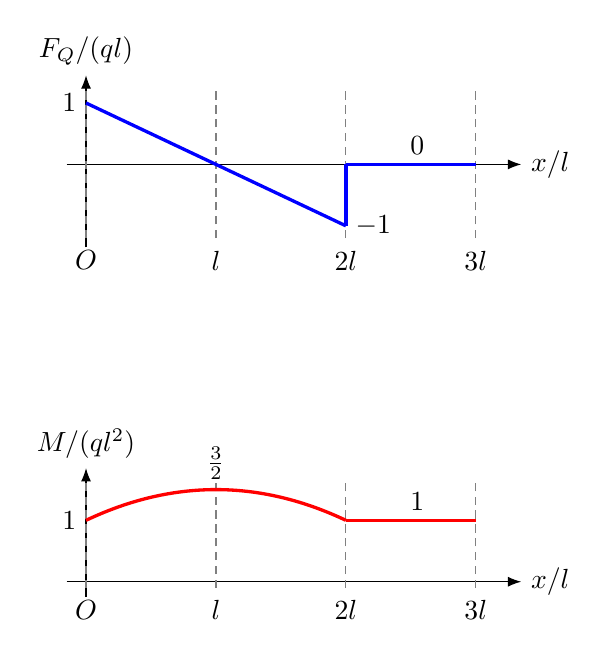
\begin{tikzpicture}[x=1.65cm,y=0.78cm,>=Latex]
  \draw[->] (-0.15,0) -- (3.35,0) node[right] {$x/l$};
  \draw[->] (0,-1.35) -- (0,1.45) node[above] {$F_Q/(ql)$};
  \foreach \x/\lab in {0/O,1/{l},2/{2l},3/{3l}}{
    \draw[densely dashed,gray] (\x,-1.2)--(\x,1.2);
    \node[below] at (\x,-1.25) {$\lab$};
  }
  \draw[very thick,blue] (0,1)--(2,-1);
  \draw[very thick,blue] (2,-1)--(2,0);
  \draw[very thick,blue] (2,0)--(3,0);
  \node[left] at (0,1) {$1$};
  \node[right] at (2,-1) {$-1$};
  \node[above] at (2.55,0) {$0$};

  \begin{scope}[yshift=-5.3cm]
    \draw[->] (-0.15,0) -- (3.35,0) node[right] {$x/l$};
    \draw[->] (0,-0.25) -- (0,1.85) node[above] {$M/(ql^2)$};
    \foreach \x/\lab in {0/O,1/{l},2/{2l},3/{3l}}{
      \draw[densely dashed,gray] (\x,-0.1)--(\x,1.65);
      \node[below] at (\x,-0.15) {$\lab$};
    }
    \draw[very thick,red,domain=0:2,samples=80] plot (\x,{1+\x-0.5*\x*\x});
    \draw[very thick,red] (2,1)--(3,1);
    \node[left] at (0,1) {$1$};
    \node[above] at (1,1.5) {$\frac32$};
    \node[above] at (2.55,1) {$1$};
  \end{scope}
\end{tikzpicture}
\caption{题 1 剪力图和弯矩图}
\end{figure}


% \newpage removed


\section*{2. 移动载荷作用下简支梁的内力分析 (25 分)}

\textbf{如图所示，某人体重为 $P$，从梁的 A 端走向 B 端。试写出他在任意位置 $x$ 时，梁的剪力和弯矩表达式；求出当弯矩取最大值时该人所在的位置，并画出相应的剪力图和弯矩图。}

\subsubsection*{解答：}

以 A 点为原点 $O$。简支梁 A 支座在 $y=0$ 处，中右部支座在 $y=2l$ 处，右端 B 为自由端在 $y=3l$ 处。
人体重为 $P$（向下），其所在位置为 $y=x$（$0 \le x \le 3l$）。

首先求支座反力 $R_A$ 和 $R_C$（以向上为正）：
\noindent\textbullet\ 绕支座 $C$ ($y=2l$) 力矩平衡：
  \[
  R_A \cdot 2l - P(2l-x) = 0 \implies R_A = P\left(1 - \frac{x}{2l}\right)
  \]
\noindent\textbullet\ 竖向受力平衡：
  \[
  R_C = P - R_A = \frac{Px}{2l}
  \]

下面按人所在位置 $x$ 的不同讨论梁截面 $y$ 上的内力：

\textbf{第一种情况：人位于支座之间 ($0 \le x \le 2l$)}
\noindent\textbullet\ 当 $0 < y < x$ 时：
  \[
  Q(y) = R_A = P\left(1 - \frac{x}{2l}\right), \quad M(y) = P\left(1 - \frac{x}{2l}\right)y
  \]
\noindent\textbullet\ 当 $x < y < 2l$ 时：
  \[
  Q(y) = R_A - P = -\frac{Px}{2l}, \quad M(y) = Px\left(1 - \frac{y}{2l}\right)
  \]
\noindent\textbullet\ 当 $2l < y < 3l$ 时：
  \[
  Q(y) = 0, \quad M(y) = 0
  \]
此时，梁上最大弯矩发生在人所在位置 $y=x$：
\[
M_{\max}(x) = Px\left(1 - \frac{x}{2l}\right)
\]
对其求导求极值点：$\frac{\diff M_{\max}}{\diff x} = P\left(1 - \frac{x}{l}\right) = 0 \implies x = l$。
即当人位于 AC 中点时，梁上最大弯矩取得局部最大值 $M_{\max, 1} = \frac{Pl}{2}$。

\textbf{第二种情况：人位于悬臂段 ($2l < x \le 3l$)}
\noindent\textbullet\ 当 $0 < y < 2l$ 时：
  \[
  Q(y) = R_A = P\left(1 - \frac{x}{2l}\right) < 0, \quad M(y) = P\left(1 - \frac{x}{2l}\right)y
  \]
\noindent\textbullet\ 当 $2l < y < x$ 时：
  \[
  Q(y) = R_A + R_C = P, \quad M(y) = P(y-x)
  \]
\noindent\textbullet\ 当 $x < y < 3l$ 时：
  \[
  Q(y) = 0, \quad M(y) = 0
  \]
此时，弯矩的绝对值最大值发生在支座 $C$ ($y=2l$) 处：
\[
|M(2l)| = P(x-2l)
\]
显然当人走到最右端 B 点 ($x=3l$) 时，取得最大值：
\[
|M|_{\max, 2} = Pl
\]

\textbf{结论}：整个过程中，弯矩最大值发生在人位于 B 端 ($x=3l$) 时，最大弯矩为 $Pl$（发生在支座 $C$ 处）。另一个局部极大值发生在人位于 AC 中点 ($x=l$) 时，最大弯矩为 $\frac{Pl}{2}$（发生在人脚下）。

当最大弯矩发生时，$x=3l$，支反力为
\[
R_A=-\frac{P}{2},\qquad R_C=\frac{3P}{2}.
\]
相应剪力图和弯矩图如下。

\begin{figure}[H]
\centering
\begin{tikzpicture}[x=1.75cm,y=0.85cm,>=Latex]
  \draw[->] (-0.15,0) -- (3.35,0) node[right] {$y/l$};
  \draw[->] (0,-0.9) -- (0,1.35) node[above] {$Q/P$};
  \foreach \x/\lab in {0/A,2/C,3/B}{
    \draw[densely dashed,gray] (\x,-0.75)--(\x,1.15);
    \node[below] at (\x,-0.8) {$\lab$};
  }
  \draw[very thick,blue] (0,-0.5)--(2,-0.5);
  \draw[very thick,blue] (2,-0.5)--(2,1);
  \draw[very thick,blue] (2,1)--(3,1);
  \draw[very thick,blue] (3,1)--(3,0);
  \node[left] at (0,-0.5) {$-\frac12$};
  \node[above] at (2.5,1) {$1$};

  \begin{scope}[yshift=-4.9cm]
    \draw[->] (-0.15,0) -- (3.35,0) node[right] {$y/l$};
    \draw[->] (0,-1.25) -- (0,0.45) node[above] {$M/(Pl)$};
    \foreach \x/\lab in {0/A,2/C,3/B}{
      \draw[densely dashed,gray] (\x,-1.05)--(\x,0.25);
      \node[below] at (\x,-1.1) {$\lab$};
    }
    \draw[very thick,red] (0,0)--(2,-1)--(3,0);
    \node[left] at (0,0) {$0$};
    \node[below] at (2,-1) {$-1$};
    \node[above] at (3,0) {$0$};
  \end{scope}
\end{tikzpicture}
\caption{题 2 最大弯矩工况的剪力图和弯矩图}
\end{figure}


% \newpage removed


\section*{3. 斜向力作用下悬臂梁的正应力计算 (25 分)}

\textbf{矩形截面悬臂梁（1200mm $\times$ 200mm $\times$ 120mm）左端固定，右端中心施加面内沿 $\theta = 30^\circ$ 方向的集中力 $F_p = 100\text{ KN}$。试求固定端截面上 A、B、C、D 四点的正应力。}

\subsubsection*{解答：}

本题按斜弯曲处理。题中说力作用在端面内，因此 $F_p$ 不产生轴力，而应分解为截面内的 $y,z$ 两个横向分量。取 $y$ 向上，$z$ 沿图中 $200\text{ mm}$ 宽度方向，A、B 位于 $-z$ 侧，C、D 位于 $+z$ 侧。
\[
F_y=F_p\cos30^\circ=86.60\text{ kN},\qquad
F_z=F_p\sin30^\circ=50.00\text{ kN}.
\]

固定端弯矩和截面惯性矩为
\[
M_z=F_yL=103.92\text{ kN}\cdot\text{m},\qquad
M_y=F_zL=60.00\text{ kN}\cdot\text{m},
\]
\[
I_z=\frac{200\times120^3}{12}=2.88\times10^7\text{ mm}^4,\qquad
I_y=\frac{120\times200^3}{12}=8.00\times10^7\text{ mm}^4.
\]
两个弯曲分量在边缘处产生的正应力大小分别为
\[
\frac{M_z(120/2)}{I_z}=216.5\text{ MPa},\qquad
\frac{M_y(200/2)}{I_y}=75.0\text{ MPa}.
\]

按图示方向，$F_y$ 使下缘受拉、上缘受压，$F_z$ 使 A、B 侧受拉，C、D 侧受压，所以
\[
\begin{aligned}
\sigma_A&=+216.5+75.0=+291.5\text{ MPa},\\
\sigma_B&=-216.5+75.0=-141.5\text{ MPa},\\
\sigma_C&=-216.5-75.0=-291.5\text{ MPa},\\
\sigma_D&=+216.5-75.0=+141.5\text{ MPa}.
\end{aligned}
\]


% \newpage removed


\section*{4. 拉弯扭组合变形下的应变分析 (25 分)}

\textbf{已知实心圆轴的直径 $d$、弹性模量 $E$ 和泊松比 $\nu$，设圆轴在自由端承受外轴向力 $P$ 和外扭转力偶 $M=Pd$ 联合作用。试求在圆轴外表面任意一点沿与纵向线呈 $45^\circ$ 方向的正应变。}

\subsubsection*{解答：}

圆轴外表面任意一点处的应力分量为：
\noindent\textbullet\ 轴向正应力：$\sigma_x = \frac{P}{A} = \frac{4P}{\pi d^2}$（拉应力）。
\noindent\textbullet\ 环向正应力：$\sigma_y = 0$。
\noindent\textbullet\ 剪应力：由扭矩 $T = M = Pd$ 产生：
  \[
  \tau_{xy} = \frac{T R}{I_p} = \frac{Pd \cdot (d/2)}{\pi d^4 / 32} = \frac{16P}{\pi d^2}
  \]

由广义胡克定律得到外表面应变分量为：
\[
\epsilon_x = \frac{1}{E} (\sigma_x - \nu \sigma_y) = \frac{4P}{\pi d^2 E}
\]
\[
\epsilon_y = \frac{1}{E} (\sigma_y - \nu \sigma_x) = -\frac{4\nu P}{\pi d^2 E}
\]
\[
\gamma_{xy} = \frac{\tau_{xy}}{G} = \frac{2(1+\nu)\tau_{xy}}{E} = \frac{32(1+\nu)P}{\pi d^2 E}
\]

对于与纵轴线呈 $\phi = 45^\circ$ 方向的线应变 $\epsilon_{45^\circ}$：
\[
\epsilon_{45^\circ} = \frac{\epsilon_x + \epsilon_y}{2} + \frac{\gamma_{xy}}{2}
\]
将分量代入可得：
\[
\epsilon_{45^\circ} = \frac{2P}{\pi d^2 E} (1 - \nu) + \frac{16(1+\nu)P}{\pi d^2 E} = \frac{2P}{\pi d^2 E} \left[ 1 - \nu + 8(1 + \nu) \right] = \frac{2P}{\pi d^2 E} (7\nu + 9)
\]
对于另一个呈 $\phi = -45^\circ$ 方向的线应变 $\epsilon_{-45^\circ}$：
\[
\epsilon_{-45^\circ} = \frac{\epsilon_x + \epsilon_y}{2} - \frac{\gamma_{xy}}{2} = -\frac{2P}{\pi d^2 E} (9\nu + 7)
\]


}

\chapter{2009 材料力学模拟试卷及答案六套题 A 卷解答}
{
\renewcommand{\assetdir}{../../考题_按知识点整理/visual_assets/question_crops/2009_2009材料力学模拟试卷及答案六套题}


\vspace{-1.0cm}

\section*{题源核查说明}

本文件整理 `2009材料力学模拟试卷及答案六套题.pdf` 中 A 卷解答。选择题、填空题按题源校对；计算题补足必要方程、符号说明和可直接照画的内力图。B--F 卷已另建独立解答文件。

\section*{一、选择题}

\begin{center}
\begin{tabular}{c c c c c}
\toprule
题号 & 1 & 2 & 3 & 4\\
\midrule
答案 & C & B & B & D\\
\bottomrule
\end{tabular}
\end{center}

其中第 1 题小变形扭转关系为
\[
    \gamma=\frac{r\varphi}{l},\qquad
    M_T=\frac{GI_p}{l}\varphi=\frac{GI_p}{r}\gamma,
    \qquad
    \varphi=\frac{l}{r}\gamma .
\]

第 2 题利用平面应力不变量：
\[
    \sigma_1+\sigma_2=\sigma_x+\sigma_y.
\]

第 3 题两点 C、D 对称，两个相同集中力共用同一个参数 $F$ 时，
\[
    \frac{\mathrm d U}{\mathrm d F}=f_C+f_D=2f_C,
    \qquad
    f_C=f_D=\frac{1}{2}\frac{\mathrm d U}{\mathrm d F}.
\]
若把两力先记为独立的 $F_C,F_D$，则应分别写
\[
    f_C=\frac{\partial U}{\partial F_C},\qquad
    f_D=\frac{\partial U}{\partial F_D}.
\]

第 4 题按两构架竖杆受压稳定控制关系判断，正确组合为 2、3，即选 D。

\section*{二、填空题}

\begin{enumerate}
    \item 强度；刚度。
    \item 剪切面面积为
    \[
        A_s=4at,
    \]
    挤压面面积为
    \[
        A_{bs}=a^2.
    \]
    \item 由已知基本梁的端部转角叠加可得
    \[
        \theta_C=\frac{q l^3}{8EI}.
    \]
    \item 因 $z_2$ 与 $z_1$ 为同一形心主轴方向，题给
    \[
        I_{z1}=\frac{bh^3}{12},
    \]
    故
    \[
        I_{z2}=I_{z1}=\frac{bh^3}{12}.
    \]
\end{enumerate}

\section*{三、计算题}

\subsection*{1. 静不定刚体-杆系：列方程求 $F_{N1}$ 与 $F_{N2}$}

\textbf{题图：}
\begin{center}
\includegraphics[width=0.48\linewidth]{\assetdir/q-009.png}
\end{center}

取刚体 AB 为研究对象，对 A 点列力矩平衡。按题图距离，外力 $F$ 的力臂为 $3a$，1 杆竖向分力力臂为 $a$，2 杆竖向分力为 $F_{N2}\cos\alpha$、力臂为 $2a$，故
\[
    \sum M_A=0:\qquad
    3F-2F_{N2}\cos\alpha-F_{N1}=0.
\]

由刚体转动几何关系，2 杆连接点竖向位移为 1 杆连接点竖向位移的 2 倍。2 杆轴向伸长在竖向的投影为 $\Delta l_2/\cos\alpha$，所以
\[
    \frac{\Delta l_2}{\cos\alpha}=2\Delta l_1.
\]

两杆 $EA$ 相同，1 杆长度为 $l$，2 杆长度为 $l/\cos\alpha$，因此
\[
    \Delta l_1=\frac{F_{N1}l}{EA},\qquad
    \Delta l_2=\frac{F_{N2}(l/\cos\alpha)}{EA}.
\]
代入协调条件：
\[
    \frac{F_{N2}l}{EA\cos^2\alpha}
    =
    \frac{2F_{N1}l}{EA},
    \qquad
    F_{N2}=2F_{N1}\cos^2\alpha.
\]

联立可得
\[
    F_{N1}=\frac{3F}{1+4\cos^3\alpha},\qquad
    F_{N2}=\frac{6F\cos^2\alpha}{1+4\cos^3\alpha}.
\]

\subsection*{2. 作梁的剪力图与弯矩图}

\textbf{题图：}
\begin{center}
\includegraphics[width=0.62\linewidth]{\assetdir/q-010.png}
\end{center}

梁两端为简支，总长 $2a$。左半跨受向下均布载荷 $q$，右半跨受向上均布载荷 $q$，跨中有集中力偶 $qa^2$。全梁竖向合力为零，且题图集中力偶与两半跨均布载荷对支座的合力矩相抵消，故
\[
    R_A=0,\qquad R_B=0.
\]

取 $x$ 自左端起，剪力方程为
\[
F_S(x)=
\begin{cases}
-qx, & 0<x<a,\\
q(x-2a), & a<x<2a.
\end{cases}
\]
因此剪力图为全负三角形，跨中处
\[
    F_S(a)=-qa.
\]

按本答案采用的弯矩正负号，跨中集中力偶使弯矩图在 $x=a$ 处发生大小为 $qa^2$ 的突变。弯矩方程可写为
\[
M(x)=
\begin{cases}
\dfrac{q x^2}{2}, & 0<x<a,\\[6pt]
-\dfrac{q(2a-x)^2}{2}, & a<x<2a.
\end{cases}
\]
关键值为
\[
    M(0)=0,\qquad M(a^-)=+\frac{qa^2}{2},\qquad
    M(a^+)=-\frac{qa^2}{2},\qquad M(2a)=0.
\]

剪力图和弯矩图如下：
\begin{center}
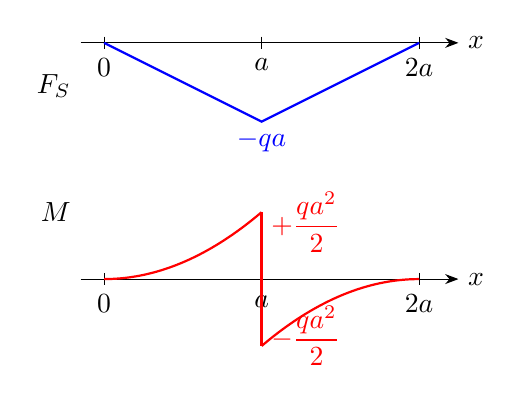
\begin{tikzpicture}[x=2.0cm,y=1.0cm,>=Stealth]
    \draw[->] (-0.15,0) -- (2.25,0) node[right] {$x$};
    \foreach \x/\lab in {0/0,1/a,2/2a}{
        \draw (\x,0.08) -- (\x,-0.08) node[below] {$\lab$};
    }
    \node[left] at (-0.15,-0.55) {$F_S$};
    \draw[thick,blue] (0,0) -- (1,-1) -- (2,0);
    \node[blue] at (1,-1.25) {$-qa$};

    \begin{scope}[yshift=-3.0cm]
        \draw[->] (-0.15,0) -- (2.25,0) node[right] {$x$};
        \foreach \x/\lab in {0/0,1/a,2/2a}{
            \draw (\x,0.08) -- (\x,-0.08) node[below] {$\lab$};
        }
        \node[left] at (-0.15,0.85) {$M$};
        \draw[thick,red,domain=0:1,samples=40] plot(\x,{0.85*\x*\x});
        \draw[thick,red] (1,0.85) -- (1,-0.85);
        \draw[thick,red,domain=1:2,samples=40] plot(\x,{-0.85*(2-\x)*(2-\x)});
        \node[red,right] at (1,0.72) {$+\dfrac{qa^2}{2}$};
        \node[red,right] at (1,-0.72) {$-\dfrac{qa^2}{2}$};
    \end{scope}
\end{tikzpicture}
\end{center}

\subsection*{3. T 形铸铁外伸梁许用载荷与合理放置}

\textbf{题图：}
\begin{center}
\includegraphics[width=0.68\linewidth]{\assetdir/q-011.png}
\end{center}

支座位于 A、B，$AB=2\text{ m}$，$BD=1\text{ m}$；C 点有集中力 $2F$，D 点有集中力 $F$。由平衡方程
\[
    R_A+R_B=3F,\qquad
    \sum M_A=0:\quad 2R_B-2F\cdot1-F\cdot3=0,
\]
得
\[
    R_B=2.5F,\qquad R_A=0.5F.
\]

关键弯矩为
\[
    M_C=R_A\cdot1=0.5F\ \text{kN}\cdot\text{m},
    \qquad
    |M_B|=F\ \text{kN}\cdot\text{m}.
\]

图 (a) 放置时，按弯矩图判断，C 截面下缘受拉，B 截面上缘受拉。由拉应力控制：
\[
    \sigma_{t,C}=\frac{M_Cy_2}{I_z}\le[\sigma_t],
    \qquad
    \sigma_{t,B}=\frac{|M_B|y_1}{I_z}\le[\sigma_t].
\]
代入
\[
    [\sigma_t]=35\text{ MPa},\quad
    I_z=5000\times10^4\text{ mm}^4,\quad
    y_1=70\text{ mm},\quad y_2=130\text{ mm},
\]
得
\[
    F\le 26.9\text{ kN}\quad(C\text{ 截面}),
    \qquad
    F\le 25.0\text{ kN}\quad(B\text{ 截面}).
\]
所以
\[
    [F]=25.0\text{ kN}.
\]

若按图 (b) 放置，$B$ 截面受拉边缘距离变为 $y_2=130\text{ mm}$，由拉应力控制约得
\[
    F\le 13.5\text{ kN}.
\]
该值小于图 (a) 的 $25.0\text{ kN}$，所以图 (a) 放置合理。

\subsection*{4. 第四强度理论确定传动轴直径}

\textbf{题图：}
\begin{center}
\includegraphics[width=0.70\linewidth]{\assetdir/q-012.png}
\end{center}

皮带轮位于两支承中点。两皮带拉力均向上，轮重向下，因此中点处竖向合力为
\[
    F_v=F_{T1}+F_{T2}-F_W
    =6+3-1=8\text{ kN}.
\]
最大弯矩出现在跨中：
\[
    M_0=\frac{F_v l}{4}
    =\frac{8\times1.6}{4}
    =3.2\text{ kN}\cdot\text{m}.
\]

传递扭矩为
\[
    M_T=(F_{T1}-F_{T2})\frac{D}{2}
    =(6-3)\times0.6
    =1.8\text{ kN}\cdot\text{m}.
\]

圆轴危险点处
\[
    \sigma=\frac{32M_0}{\pi d^3},
    \qquad
    \tau=\frac{16M_T}{\pi d^3}.
\]
按第四强度理论：
\[
    \sigma_{r4}
    =
    \sqrt{\sigma^2+3\tau^2}
    =
    \frac{32}{\pi d^3}
    \sqrt{M_0^2+\frac34M_T^2}
    \le[\sigma].
\]
因此
\[
    d\ge
    \left[
    \frac{32\sqrt{M_0^2+\frac34M_T^2}}
    {\pi[\sigma]}
    \right]^{1/3}.
\]
代入 $M_0=3.2\times10^6\text{ N}\cdot\text{mm}$、$M_T=1.8\times10^6\text{ N}\cdot\text{mm}$、$[\sigma]=50\text{ MPa}$：
\[
    d\ge
    \left[
    \frac{32\sqrt{(3.2\times10^6)^2+\frac34(1.8\times10^6)^2}}
    {\pi\times50}
    \right]^{1/3}
    =
    89.8\text{ mm}.
\]

故传动轴直径应取
\[
    d\ge 89.8\text{ mm}.
\]


}

\chapter{2009 材料力学模拟试卷及答案六套题 B 卷解答}
{
\renewcommand{\assetdir}{../../考题_按知识点整理/visual_assets/question_crops/2009_2009材料力学模拟试卷及答案六套题}


\vspace{-1.0cm}

\section*{题源核查说明}

本文件整理 `2009材料力学模拟试卷及答案六套题.pdf` 中 B 卷解答。选择题、填空题按题源校对；证明题和计算题补足必要方程、符号说明和内力图关键值。

\section*{一、选择题}

\begin{center}
\begin{tabular}{c c}
\toprule
题号 & 1\\
\midrule
答案 & B\\
\bottomrule
\end{tabular}
\end{center}

纯弯曲条件下，中性轴通过横截面的形心，故选 B。

\section*{二、填空题}

\begin{enumerate}
    \item 连续性假设；均匀性假设；各向同性假设。
    \item 强度；刚度。
    \item 螺栓杆身拉伸面积为
    \[
        A_t=\frac{\pi d^2}{4},
    \]
    螺栓头剪切面面积为
    \[
        A_\tau=\pi d h.
    \]
    由
    \[
        \frac{F}{A_t}\le [\sigma],\qquad
        \frac{F}{A_\tau}\le [\tau]=0.6[\sigma],
    \]
    两者同时达到许用值时
    \[
        \frac{4F/(\pi d^2)}{F/(\pi d h)}
        =\frac{1}{0.6},
        \qquad
        \frac{d}{h}=2.4.
    \]
\end{enumerate}

\section*{三、证明题}

\subsection*{1. 均布载荷梁支座间距的最优位置}

\textbf{题图：}
\begin{center}
\includegraphics[width=0.72\linewidth]{\assetdir/q-029.png}
\end{center}

设梁总长为 $l$，两个对称支座间距为 $a$。由对称性，两端外伸长度均为
\[
    c=\frac{l-a}{2}.
\]

支座处负弯矩为
\[
    M_B=-\frac{q c^2}{2}
    =-\frac{q}{2}\left(\frac{l-a}{2}\right)^2.
\]
跨中正弯矩为
\[
    M_x=\frac{qla}{4}-\frac{ql^2}{8}.
\]
要使横截面内最大弯矩的绝对值达到最小，应使最大正弯矩与最大负弯矩等值：
\[
    -M_B=M_x.
\]
代入得
\[
    \frac{q}{2}\left(\frac{l-a}{2}\right)^2
    =\frac{qla}{4}-\frac{ql^2}{8},
\]
\[
    a^2-4la+2l^2=0.
\]
因 $0<a<l$，取
\[
    a=(2-\sqrt{2})l.
\]

\subsection*{2. 同截面梁弯成同心圆弧后的最大正应力比较}

\textbf{题图：}
\begin{center}
\includegraphics[width=0.72\linewidth]{\assetdir/q-031.png}
\end{center}

纯弯曲时，梁轴线曲率与最大边缘应变满足
\[
    \varepsilon_{\max}=\frac{y_{\max}}{\rho}.
\]
故
\[
    (\sigma_{\max})_A
    =E(\varepsilon_{\max})_A
    =E\frac{y_{\max}}{\rho_A},
\]
\[
    (\sigma_{\max})_B
    =E(\varepsilon_{\max})_B
    =E\frac{y_{\max}}{\rho_B}.
\]
两梁材料相同、截面相同，故 $E$ 与 $y_{\max}$ 相同。题图中两梁弯成同心圆弧，A 梁的曲率半径大于 B 梁：
\[
    \rho_A>\rho_B.
\]
因此
\[
    (\sigma_{\max})_A<(\sigma_{\max})_B.
\]

\section*{四、计算题}

\subsection*{1. 刚性杆与两拉压杆}

\textbf{题图：}
\begin{center}
\includegraphics[width=0.58\linewidth]{\assetdir/q-032.png}
\end{center}

设 1 杆轴力拉力为正，2 杆轴力拉力为正。BC 为刚性杆，1、2 两杆抗拉压刚度均为 $EA$。由刚性杆平衡与两杆变形协调可得
\[
    F_{N1}=\frac{3F}{5},\qquad
    F_{N2}=-\frac{3F}{5}.
\]
所以
\[
    F_{N1}=\frac{3F}{5}\quad(\text{拉力}),\qquad
    |F_{N2}|=\frac{3F}{5}\quad(\text{压力}).
\]

\subsection*{2. 分布力偶圆轴的扭矩图与相对扭转角}

\textbf{题图：}
\begin{center}
\includegraphics[width=0.58\linewidth]{\assetdir/q-033.png}
\end{center}

AB 段长 $l/2$，受均布力偶矩 $m_q$。从 A 截面向左取截面，AB 段扭矩线性增加，B 到 C 段扭矩为常数：
\[
    M_T(x)=m_q x,\qquad 0\le x\le \frac{l}{2},
\]
\[
    M_T=\frac{m_q l}{2},\qquad \frac{l}{2}\le x\le l.
\]

\begin{center}
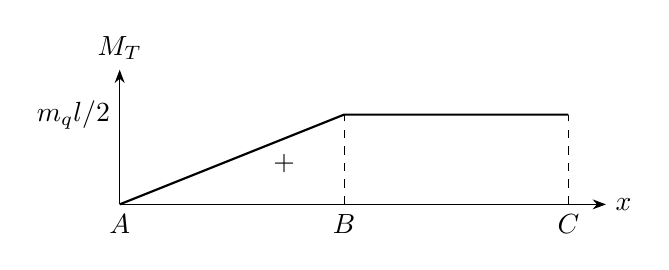
\begin{tikzpicture}[>=Stealth,scale=0.95]
    \draw[->] (0,0) -- (6.5,0) node[right] {$x$};
    \draw[->] (0,0) -- (0,1.8) node[above] {$M_T$};
    \draw[thick] (0,0) -- (3,1.2) -- (6,1.2);
    \draw[dashed] (3,0) node[below] {$B$} -- (3,1.2);
    \draw[dashed] (6,0) node[below] {$C$} -- (6,1.2);
    \node[below] at (0,0) {$A$};
    \node[left] at (0,1.2) {$m_q l/2$};
    \node at (2.2,0.55) {$+$};
\end{tikzpicture}
\end{center}

圆截面极惯性矩为
\[
    I_p=\frac{\pi d^4}{32}.
\]
A、C 两截面间相对扭转角为
\[
    \varphi_{AC}
    =\frac{1}{GI_p}
    \left[
        \int_0^{l/2}m_q x\,dx
        +\frac{m_q l}{2}\cdot\frac{l}{2}
    \right]
\]
\[
    =\frac{1}{GI_p}
    \left(
        \frac{m_q l^2}{8}
        +\frac{m_q l^2}{4}
    \right)
    =\frac{3m_q l^2}{8GI_p}
    =\frac{12m_q l^2}{G\pi d^4}.
\]

\subsection*{3. 悬臂梁剪力图与弯矩图}

\textbf{题图：}
\begin{center}
\includegraphics[width=0.62\linewidth]{\assetdir/q-034.png}
\end{center}

取固定端为 $x=0$，自由端为 $x=3a$，向上分布载荷为正。固定端反力为
\[
    R_A=qa.
\]
剪力方程为
\[
    F_S(x)=q(x-a),\qquad 0\le x\le 2a,
\]
\[
    F_S(x)=q(3a-x),\qquad 2a\le x\le 3a.
\]
弯矩方程为
\[
    M(x)=-qa^2+\frac{q}{2}(x-a)^2,\qquad 0\le x\le 2a,
\]
\[
    M(x)=-\frac{q}{2}(3a-x)^2,\qquad 2a\le x\le 3a.
\]

关键值为
\[
    F_S(0)=-qa,\quad F_S(a)=0,\quad F_S(2a)=qa,\quad F_S(3a)=0,
\]
\[
    M(0)=-\frac{qa^2}{2},\quad M(a)=-qa^2,\quad
    M(2a)=-\frac{qa^2}{2},\quad M(3a)=0.
\]
可直接按下图誊画：

\begin{center}
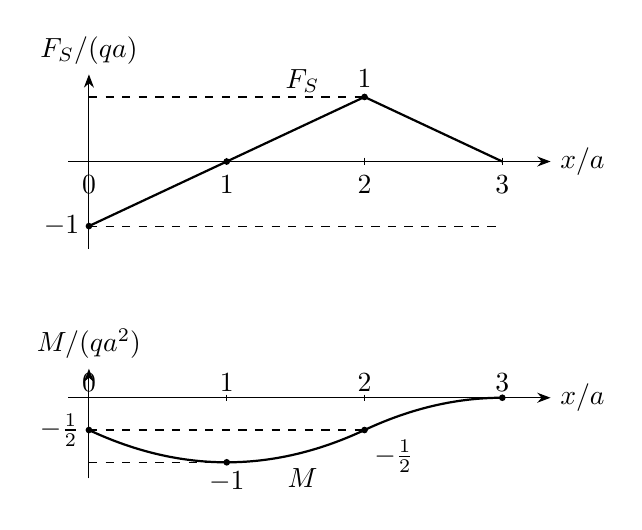
\begin{tikzpicture}[x=1.75cm,y=0.82cm,>=Stealth]
    \begin{scope}
        \draw[->] (-0.15,0) -- (3.35,0) node[right] {$x/a$};
        \draw[->] (0,-1.35) -- (0,1.35) node[above] {$F_S/(qa)$};
        \foreach \x/\lab in {0/0,1/1,2/2,3/3}{
            \draw (\x,0.06)--(\x,-0.06) node[below] {$\lab$};
        }
        \draw[dashed] (0,-1)--(3,-1);
        \draw[dashed] (0,1)--(2,1);
        \draw[thick] (0,-1)--(2,1)--(3,0);
        \fill (0,-1) circle (1.2pt) node[left] {$-1$};
        \fill (1,0) circle (1.2pt);
        \fill (2,1) circle (1.2pt) node[above] {$1$};
        \node at (1.55,1.25) {$F_S$};
    \end{scope}
    \begin{scope}[yshift=-3.0cm]
        \draw[->] (-0.15,0) -- (3.35,0) node[right] {$x/a$};
        \draw[->] (0,-1.25) -- (0,0.45) node[above] {$M/(qa^2)$};
        \foreach \x/\lab in {0/0,1/1,2/2,3/3}{
            \draw (\x,0.05)--(\x,-0.05) node[above] {$\lab$};
        }
        \draw[dashed] (0,-0.5)--(2,-0.5);
        \draw[dashed] (0,-1)--(1,-1);
        \draw[thick,domain=0:2,samples=80] plot (\x,{-1+0.5*(\x-1)^2});
        \draw[thick,domain=2:3,samples=60] plot (\x,{-0.5*(3-\x)^2});
        \fill (0,-0.5) circle (1.2pt) node[left] {$-\frac12$};
        \fill (1,-1) circle (1.2pt) node[below] {$-1$};
        \fill (2,-0.5) circle (1.2pt) node[below right] {$-\frac12$};
        \fill (3,0) circle (1.2pt);
        \node at (1.55,-1.25) {$M$};
    \end{scope}
\end{tikzpicture}
\end{center}

\subsection*{4. 外伸梁剪力图与弯矩图}

\textbf{题图：}
\begin{center}
\includegraphics[width=0.70\linewidth]{\assetdir/q-035.png}
\end{center}

取 A 点为 $x=0$，B 点为 $x=10\text{ m}$，右端为 $x=12\text{ m}$。均布载荷从 $x=2\text{ m}$ 到 $x=12\text{ m}$，大小为 $20\text{ kN/m}$；右端集中力为 $20\text{ kN}$。由整体平衡得
\[
    F_A=80\text{ kN}\quad(\uparrow),\qquad
    F_B=140\text{ kN}\quad(\uparrow).
\]

剪力方程为
\[
    F_S=80,\qquad 0<x<2,
\]
\[
    F_S=80-20(x-2)=120-20x,\qquad 2<x<10,
\]
\[
    F_S=80+140-20(x-2)=260-20x,\qquad 10<x<12.
\]
在右端集中力处，剪力由 $20\text{ kN}$ 跳至 0。

弯矩方程为
\[
    M=80x,\qquad 0<x<2,
\]
在 $x=2\text{ m}$ 处受 $240\text{ kN}\cdot\text{m}$ 集中力偶，弯矩图发生突跳。按题图力偶方向取
\[
    M(2^-)=160\text{ kN}\cdot\text{m},\qquad
    M(2^+)=-80\text{ kN}\cdot\text{m}.
\]
之后
\[
    M=-10x^2+120x-280,\qquad 2<x<10,
\]
\[
    M=-10x^2+260x-1680,\qquad 10<x<12.
\]
关键值为
\[
    M(6)=80\text{ kN}\cdot\text{m},\qquad
    M(10)=-80\text{ kN}\cdot\text{m},\qquad
    M(12)=0.
\]

可直接按下图誊画，注意 $x=2\text{ m}$ 处弯矩因集中力偶由 $160$ 突跳到 $-80$：
\begin{center}
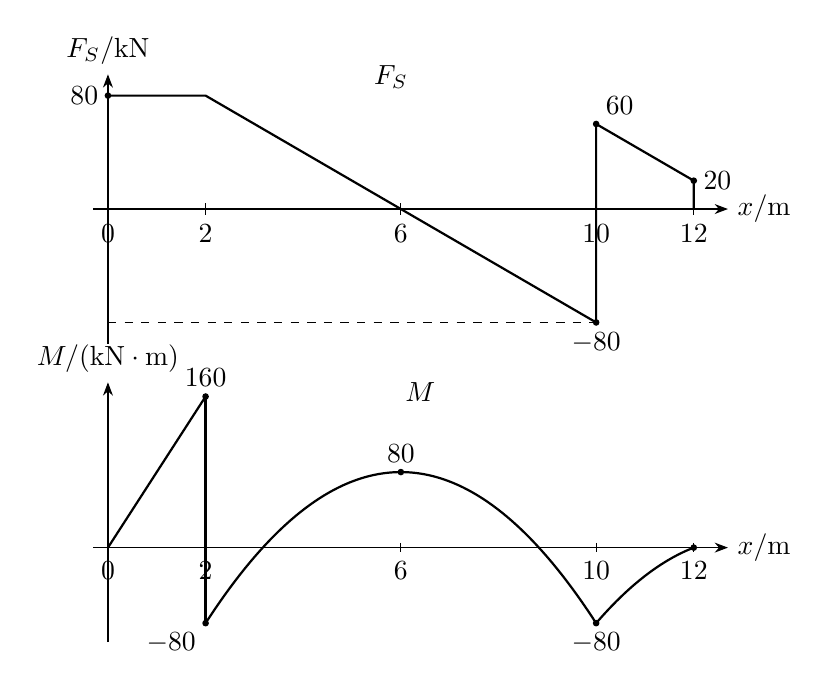
\begin{tikzpicture}[x=0.62cm,>=Stealth]
    \begin{scope}[y=0.018cm]
        \draw[->] (-0.3,0) -- (12.7,0) node[right] {$x/\text{m}$};
        \draw[->] (0,-95) -- (0,95) node[above] {$F_S/\text{kN}$};
        \foreach \x/\lab in {0/0,2/2,6/6,10/10,12/12}{
            \draw (\x,4)--(\x,-4) node[below] {$\lab$};
        }
        \draw[dashed] (0,80)--(2,80);
        \draw[dashed] (0,-80)--(10,-80);
        \draw[thick] (0,80)--(2,80)--(10,-80);
        \draw[thick] (10,-80)--(10,60)--(12,20)--(12,0);
        \fill (0,80) circle (1.2pt) node[left] {$80$};
        \fill (10,-80) circle (1.2pt) node[below] {$-80$};
        \fill (10,60) circle (1.2pt) node[above right] {$60$};
        \fill (12,20) circle (1.2pt) node[right] {$20$};
        \node at (5.8,93) {$F_S$};
    \end{scope}
    \begin{scope}[yshift=-4.3cm,y=0.012cm]
        \draw[->] (-0.3,0) -- (12.7,0) node[right] {$x/\text{m}$};
        \draw[->] (0,-100) -- (0,175) node[above] {$M/(\text{kN}\cdot\text{m})$};
        \foreach \x/\lab in {0/0,2/2,6/6,10/10,12/12}{
            \draw (\x,5)--(\x,-5) node[below] {$\lab$};
        }
        \draw[thick] (0,0)--(2,160);
        \draw[thick] (2,160)--(2,-80);
        \draw[thick,domain=2:10,samples=80] plot (\x,{-10*\x*\x+120*\x-280});
        \draw[thick,domain=10:12,samples=50] plot (\x,{-10*\x*\x+260*\x-1680});
        \fill (2,160) circle (1.2pt) node[above] {$160$};
        \fill (2,-80) circle (1.2pt) node[below left] {$-80$};
        \fill (6,80) circle (1.2pt) node[above] {$80$};
        \fill (10,-80) circle (1.2pt) node[below] {$-80$};
        \fill (12,0) circle (1.2pt);
        \node at (6.4,165) {$M$};
    \end{scope}
\end{tikzpicture}
\end{center}

\subsection*{5. T 形截面梁 B 截面 K 点应力}

\textbf{题图：}
\begin{center}
\includegraphics[width=0.78\linewidth]{\assetdir/q-036.png}
\end{center}

B 截面的剪力和弯矩为
\[
    F_{SB}=-1.0\times10^4\text{ N},
\]
\[
    M_B=1.5\times10^4\text{ N}\cdot\text{m}.
\]
题给
\[
    I_z=4.03\times10^7\text{ mm}^4.
\]
截面中性轴距底边为 $61\text{ mm}$，K 点位于腹板与翼缘交界处，距底边 $30\text{ mm}$，故
\[
    y_K=61-30=31\text{ mm}.
\]
正应力为
\[
    \sigma_K=\frac{M_B y_K}{I_z}
    =\frac{1.5\times10^7\times31}{4.03\times10^7}
    =11.5\text{ MPa}.
\]

K 点切应力用弯曲剪应力公式
\[
    \tau_K=\frac{F_{SB}S_z^*(K)}{bI_z}.
\]
K 点以上为腹板面积 $30\times170\text{ mm}^2$，其形心距中性轴为
\[
    30+\frac{170}{2}-61=54\text{ mm},
\]
故
\[
    S_z^*(K)=30\times170\times54=2.754\times10^5\text{ mm}^3.
\]
取腹板宽度 $b=30\text{ mm}$，得
\[
    \tau_K
    =\frac{-1.0\times10^4\times2.754\times10^5}
    {30\times4.03\times10^7}
    =-2.28\text{ MPa}.
\]

因此 B 截面 K 点应力为
\[
    \sigma_K=11.5\text{ MPa},\qquad
    \tau_K=-2.28\text{ MPa}.
\]


}

\chapter{2009 材料力学模拟试卷及答案六套题 C 卷解答}
{
\renewcommand{\assetdir}{../../考题_按知识点整理/visual_assets/question_crops/2009_2009材料力学模拟试卷及答案六套题}


\vspace{-1.0cm}

\section*{题源核查说明}

本文件整理 `2009材料力学模拟试卷及答案六套题.pdf` 中 C 卷解答。填空题、证明题按题源校对；计算题补入关键公式、内力图关键值和应力计算。

\section*{一、填空题}

\begin{enumerate}
    \item 轴向拉伸或压缩；剪切；扭转；弯曲。
    \item 图示铆钉连接在外力作用下可能产生的破坏方式为：
    \[
        \text{铆钉被剪断；钢板或铆钉被挤压破坏；钢板端部被剪坏；钢板被拉断。}
    \]
\end{enumerate}

\section*{二、证明题}

\textbf{题图：}
\begin{center}
\includegraphics[width=0.72\linewidth]{\assetdir/q-050.png}
\end{center}

由梁内力微分关系
\[
    \frac{dM(x)}{dx}=F_S(x),
\]
对全梁积分得
\[
    \int_0^l F_S(x)\,dx
    =\int_0^l dM(x)
    =M(l)-M(0).
\]
简支梁两端铰支，端弯矩均为零：
\[
    M(0)=0,\qquad M(l)=0.
\]
因此
\[
    \int_0^l F_S(x)\,dx=0,
\]
即全梁剪力图的代数面积之和为零。

\section*{三、计算题}

\subsection*{1. 刚性梁三杆结构的许可载荷}

\textbf{题图：}
\begin{center}
\includegraphics[width=0.58\linewidth]{\assetdir/q-051.png}
\end{center}

AB 为刚性梁，三杆横截面积均为 $A$，材料许用应力为 $[\sigma]$。由刚性梁平衡与三杆变形协调可得控制杆轴力满足
\[
    F_{\max}=\frac{2}{5}F.
\]
强度条件为
\[
    \frac{F_{\max}}{A}\le [\sigma],
\]
故
\[
    \frac{2F}{5A}\le [\sigma],
    \qquad
    [F]=\frac{5[\sigma]A}{2}.
\]

\subsection*{2. 圆轴扭转求剪变模量}

已知
\[
    d=30\text{ mm}=0.03\text{ m},\qquad
    M_T=0.25\text{ kN}\cdot\text{m}=250\text{ N}\cdot\text{m},
\]
\[
    l=2\text{ m},\qquad
    \varphi=3.74^\circ=\frac{3.74\pi}{180}\text{ rad}.
\]
实心圆轴极惯性矩
\[
    I_p=\frac{\pi d^4}{32}.
\]
由扭转角公式
\[
    \varphi=\frac{M_T l}{GI_p}
\]
得
\[
    G=\frac{M_T l}{I_p\varphi}
    =96.4\text{ GPa}.
\]

\subsection*{3. 梁的剪力图和弯矩图}

\textbf{题图：}
\begin{center}
\includegraphics[width=0.62\linewidth]{\assetdir/q-053.png}
\end{center}

取左端为 $x=0$，固定端为 $x=3a$，按本解中剪力正号约定，剪力方程为
\[
    F_S=2qa,\qquad 0<x<a,
\]
\[
    F_S=q(3a-x),\qquad a<x<2a,
\]
\[
    F_S=qa,\qquad 2a<x<3a.
\]
弯矩在 $x=a$ 处受集中力偶影响发生突跳：
\[
    M=2qax,\qquad 0<x<a,
\]
\[
    M(a^-)=2qa^2,\qquad M(a^+)=-qa^2,
\]
\[
    M=q\left(-\frac{x^2}{2}+3ax-\frac{7a^2}{2}\right),\qquad a<x<2a,
\]
\[
    M=qa(x-2a)+\frac{qa^2}{2},\qquad 2a<x<3a.
\]

剪力图与弯矩图如下。抄图时保留关键值：剪力图在 $0<x<a$ 保持 $2qa$，在 $a<x<2a$ 线性降至 $qa$，右段保持 $qa$；弯矩图关键值为 $2qa^2$、$-qa^2$、$qa^2/2$ 与 $3qa^2/2$。

\begin{center}
\includegraphics[width=0.70\linewidth]{\assetdir/q-062.png}
\end{center}

重画时可按下列坐标图誊写：
\begin{center}
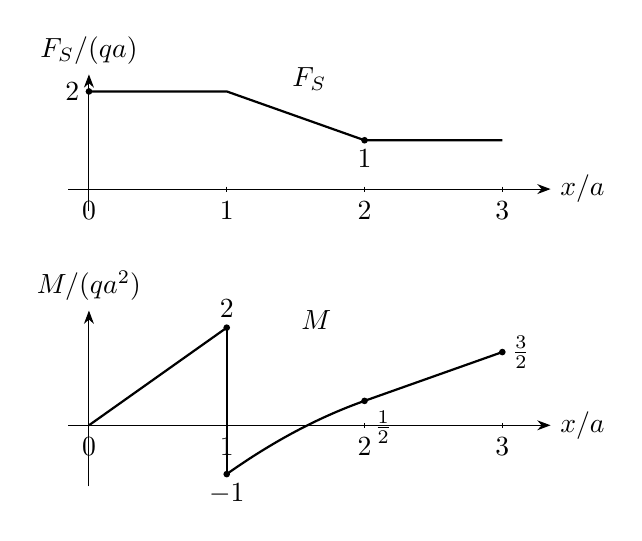
\begin{tikzpicture}[x=1.75cm,y=0.62cm,>=Stealth]
    \begin{scope}
        \draw[->] (-0.15,0) -- (3.35,0) node[right] {$x/a$};
        \draw[->] (0,-0.45) -- (0,2.35) node[above] {$F_S/(qa)$};
        \foreach \x/\lab in {0/0,1/1,2/2,3/3}{
            \draw (\x,0.05)--(\x,-0.05) node[below] {$\lab$};
        }
        \draw[thick] (0,2)--(1,2)--(2,1)--(3,1);
        \fill (0,2) circle (1.2pt) node[left] {$2$};
        \fill (2,1) circle (1.2pt) node[below] {$1$};
        \node at (1.6,2.25) {$F_S$};
    \end{scope}
    \begin{scope}[yshift=-3.0cm]
        \draw[->] (-0.15,0) -- (3.35,0) node[right] {$x/a$};
        \draw[->] (0,-1.25) -- (0,2.35) node[above] {$M/(qa^2)$};
        \foreach \x/\lab in {0/0,1/1,2/2,3/3}{
            \draw (\x,0.05)--(\x,-0.05) node[below] {$\lab$};
        }
        \draw[thick] (0,0)--(1,2);
        \draw[thick] (1,2)--(1,-1);
        \draw[thick,domain=1:2,samples=80] plot (\x,{-0.5*\x*\x+3*\x-3.5});
        \draw[thick] (2,0.5)--(3,1.5);
        \fill (1,2) circle (1.2pt) node[above] {$2$};
        \fill (1,-1) circle (1.2pt) node[below] {$-1$};
        \fill (2,0.5) circle (1.2pt) node[below right] {$\frac12$};
        \fill (3,1.5) circle (1.2pt) node[right] {$\frac32$};
        \node at (1.65,2.15) {$M$};
    \end{scope}
\end{tikzpicture}
\end{center}

\subsection*{4. 外伸梁剪力图与弯矩图}

\textbf{题图：}
\begin{center}
\includegraphics[width=0.70\linewidth]{\assetdir/q-035.png}
\end{center}

取 A 点为 $x=0$，B 点为 $x=10\text{ m}$，右端为 $x=12\text{ m}$。均布载荷从 $x=2\text{ m}$ 到 $x=12\text{ m}$，大小为 $20\text{ kN/m}$；右端集中力为 $20\text{ kN}$。由整体平衡得
\[
    F_A=80\text{ kN}\quad(\uparrow),\qquad
    F_B=140\text{ kN}\quad(\uparrow).
\]

剪力方程为
\[
    F_S=80,\qquad 0<x<2,
\]
\[
    F_S=120-20x,\qquad 2<x<10,
\]
\[
    F_S=260-20x,\qquad 10<x<12.
\]
在右端集中力处，剪力由 $20\text{ kN}$ 跳至 0。

弯矩方程为
\[
    M=80x,\qquad 0<x<2,
\]
\[
    M(2^-)=160\text{ kN}\cdot\text{m},\qquad
    M(2^+)=-80\text{ kN}\cdot\text{m},
\]
\[
    M=-10x^2+120x-280,\qquad 2<x<10,
\]
\[
    M=-10x^2+260x-1680,\qquad 10<x<12.
\]
关键值：
\[
    M(6)=80\text{ kN}\cdot\text{m},\qquad
    M(10)=-80\text{ kN}\cdot\text{m},\qquad
    M(12)=0.
\]

可直接按下图誊画，注意 $x=2\text{ m}$ 处弯矩因集中力偶由 $160$ 突跳到 $-80$：
\begin{center}
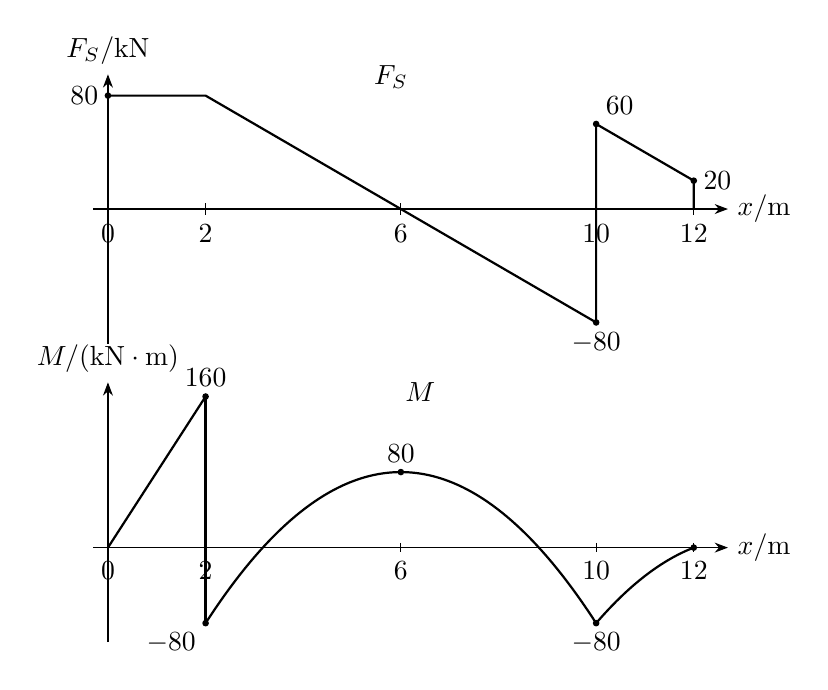
\begin{tikzpicture}[x=0.62cm,>=Stealth]
    \begin{scope}[y=0.018cm]
        \draw[->] (-0.3,0) -- (12.7,0) node[right] {$x/\text{m}$};
        \draw[->] (0,-95) -- (0,95) node[above] {$F_S/\text{kN}$};
        \foreach \x/\lab in {0/0,2/2,6/6,10/10,12/12}{
            \draw (\x,4)--(\x,-4) node[below] {$\lab$};
        }
        \draw[thick] (0,80)--(2,80)--(10,-80);
        \draw[thick] (10,-80)--(10,60)--(12,20)--(12,0);
        \fill (0,80) circle (1.2pt) node[left] {$80$};
        \fill (10,-80) circle (1.2pt) node[below] {$-80$};
        \fill (10,60) circle (1.2pt) node[above right] {$60$};
        \fill (12,20) circle (1.2pt) node[right] {$20$};
        \node at (5.8,93) {$F_S$};
    \end{scope}
    \begin{scope}[yshift=-4.3cm,y=0.012cm]
        \draw[->] (-0.3,0) -- (12.7,0) node[right] {$x/\text{m}$};
        \draw[->] (0,-100) -- (0,175) node[above] {$M/(\text{kN}\cdot\text{m})$};
        \foreach \x/\lab in {0/0,2/2,6/6,10/10,12/12}{
            \draw (\x,5)--(\x,-5) node[below] {$\lab$};
        }
        \draw[thick] (0,0)--(2,160);
        \draw[thick] (2,160)--(2,-80);
        \draw[thick,domain=2:10,samples=80] plot (\x,{-10*\x*\x+120*\x-280});
        \draw[thick,domain=10:12,samples=50] plot (\x,{-10*\x*\x+260*\x-1680});
        \fill (2,160) circle (1.2pt) node[above] {$160$};
        \fill (2,-80) circle (1.2pt) node[below left] {$-80$};
        \fill (6,80) circle (1.2pt) node[above] {$80$};
        \fill (10,-80) circle (1.2pt) node[below] {$-80$};
        \fill (12,0) circle (1.2pt);
        \node at (6.4,165) {$M$};
    \end{scope}
\end{tikzpicture}
\end{center}

\subsection*{5. T 形截面铸铁梁的最大拉压应力}

\textbf{题图：}
\begin{center}
\includegraphics[width=0.78\linewidth]{\assetdir/q-055.png}
\end{center}

由整体平衡与弯矩图可得关键弯矩：
\[
    M_B=-25\text{ kN}\cdot\text{m},\qquad
    M_{+,\max}=14.1\text{ kN}\cdot\text{m}.
\]
题给
\[
    I_z=2.59\times 10^{-5}\text{ m}^4,
    \qquad y_{\text{下}}=142\text{ mm}=0.142\text{ m}.
\]

B 截面下边缘产生最大压应力：
\[
    (\sigma_c)_{\max}
    =\frac{M_B y_{\text{下}}}{I_z}
    =\frac{-25\times10^3\times0.142}{2.59\times10^{-5}}
    =-137\text{ MPa}.
\]
AB 跨内剪力为零截面处取得最大正弯矩，该截面距 A 为 $0.75\text{ m}$。该截面下边缘产生最大拉应力：
\[
    (\sigma_t)_{\max}
    =\frac{M_{+,\max} y_{\text{下}}}{I_z}
    =\frac{14.1\times10^3\times0.142}{2.59\times10^{-5}}
    =77.3\text{ MPa}.
\]

\subsection*{6. 矩形截面梁 D 左截面 K 点应力}

\textbf{题图：}
\begin{center}
\includegraphics[width=0.78\linewidth]{\assetdir/q-056.png}
\end{center}

由整体平衡得
\[
    F_A=\frac{F}{3}\quad(\uparrow).
\]
取 D 左截面：
\[
    F_{SD}=-\frac{2F}{3},
    \qquad
    M_D=-\frac{Fa}{3}.
\]
矩形截面惯性矩
\[
    I_z=\frac{bh^3}{12}.
\]
K 点位于距中性轴 $h/4$ 处，故正应力
\[
    \sigma_K=\frac{M_D y_K}{I_z}
    =\frac{\left(-Fa/3\right)\left(h/4\right)}{bh^3/12}
    =-\frac{Fa}{bh^2}.
\]
K 点以上面积静矩代入弯曲剪应力公式
\[
    \tau_K=\frac{F_{SD}S_z^*(K)}{bI_z}
    =-\frac{3F}{4bh}.
\]


}

\chapter{2009 材料力学模拟试卷及答案六套题 D 卷解答}
{
\renewcommand{\assetdir}{../../考题_按知识点整理/visual_assets/question_crops/2009_2009材料力学模拟试卷及答案六套题}


\vspace{-1.0cm}

\section*{题源核查说明}

本文件整理 `2009材料力学模拟试卷及答案六套题.pdf` 中 D 卷解答。选择题、填空题按题源校对；计算题补足关键公式，并保留题图或内力图作为核对依据。

\section*{一、选择题}

\begin{center}
\begin{tabular}{c c c c}
\toprule
题号 & 1 & 2 & 3\\
\midrule
答案 & B & A & B\\
\bottomrule
\end{tabular}
\end{center}

\section*{二、填空题}

\begin{enumerate}
    \item 题图如下：
    \begin{center}
    \includegraphics[width=0.70\linewidth]{\assetdir/q-070.png}
    \end{center}
    边界条件：
    \[
        x=0,\quad w_1=0,\quad \theta_1=0;
        \qquad
        x=l,\quad w_2=\frac{ql}{4k}.
    \]
    连续条件：
    \[
        x=\frac{l}{2},\qquad w_1=w_2.
    \]

    \item
    \[
        w_C=0.024\,\frac{F l^3}{EI}.
    \]

    \item
    \[
        \sigma_{\alpha}=72.1\text{ MPa}.
    \]

    \item
    \[
        r_A=-1,\qquad r_B=+1,\qquad r_C=0,\qquad r_D=0,
    \]
    \[
        \sigma_{-1}=410\text{ MPa},\qquad \sigma_b=900\text{ MPa},
    \]
    \[
        \sigma_{\max}=500\text{ MPa},\qquad \sigma_{\min}=300\text{ MPa}.
    \]
\end{enumerate}

\section*{三、计算题}

\subsection*{1. 刚性梁三杆结构}

\textbf{题图：}
\begin{center}
\includegraphics[width=0.62\linewidth]{\assetdir/q-076.png}
\end{center}

设三杆轴力拉为正。刚性梁位移为直线分布，故
\[
    2\delta_2=\delta_1+\delta_3
    \quad\Rightarrow\quad
    2F_{N2}=F_{N1}+F_{N3}.
\]
整体平衡为
\[
    F_{N1}+F_{N2}+F_{N3}=F,
    \qquad
    F_{N2}a+2F_{N3}a=2Fa.
\]
联立得
\[
    F_{N1}=-\frac{F}{6},\qquad
    F_{N2}=\frac{F}{3},\qquad
    F_{N3}=\frac{5F}{6}.
\]

\subsection*{2. 圆轴扭转力偶}

\textbf{题图：}
\begin{center}
\includegraphics[width=0.62\linewidth]{\assetdir/q-077.png}
\end{center}

实心圆轴极惯性矩
\[
    I_p=\frac{\pi d^4}{32}.
\]
由扭转角公式，注意题给扭转角为角度制：
\[
    \varphi_{AB}=\frac{M_e l}{GI_p}\frac{180^\circ}{\pi}.
\]
代入 $d=36\text{ mm}$、$G=80\text{ GPa}$、$l=2\text{ m}$、$\varphi_{AB}=1.2^\circ$，得
\[
    M_e=138\text{ N}\cdot\text{m}.
\]

\subsection*{3. 梁的剪力图和弯矩图}

\textbf{题图：}
\begin{center}
\includegraphics[width=0.70\linewidth]{\assetdir/q-078.png}
\end{center}

取左端为 $x=0$，右端为 $x=3a$。按图示载荷和本解符号约定，剪力方程为
\[
    F_S=\frac{qa}{2},\qquad 0<x<a,
\]
\[
    F_S=-\frac{qa}{2},\qquad a<x<2a,
\]
\[
    F_S=q(3a-x),\qquad 2a<x<3a.
\]
弯矩图在 $x=2a$ 处因集中力偶向负侧突跳：
\[
    M=\frac{qa}{2}x,\qquad 0<x<a,
\]
\[
    M=\frac{qa^2}{2}-\frac{qa}{2}(x-a),\qquad a<x<2a,
\]
\[
    M(2a^-)=0,\qquad M(2a^+)=-\frac{qa^2}{2},
\]
\[
    M=-\frac{q}{2}(3a-x)^2,\qquad 2a<x<3a.
\]

内力图如下。抄图时保留关键值：剪力图左段为 $qa/2$，中段为 $-qa/2$，右段由 $qa$ 线性降至 0；弯矩图最大正弯矩与最大负弯矩的绝对值均为 $qa^2/2$。

\begin{center}
\includegraphics[width=0.62\linewidth]{\assetdir/q-094.png}
\end{center}

重画时可按下列坐标图誊写：
\begin{center}
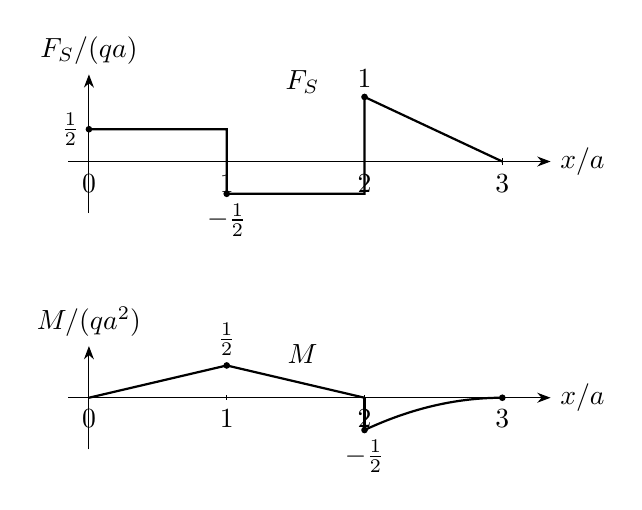
\begin{tikzpicture}[x=1.75cm,y=0.82cm,>=Stealth]
    \begin{scope}
        \draw[->] (-0.15,0) -- (3.35,0) node[right] {$x/a$};
        \draw[->] (0,-0.8) -- (0,1.35) node[above] {$F_S/(qa)$};
        \foreach \x/\lab in {0/0,1/1,2/2,3/3}{
            \draw (\x,0.05)--(\x,-0.05) node[below] {$\lab$};
        }
        \draw[thick] (0,0.5)--(1,0.5)--(1,-0.5)--(2,-0.5)--(2,1)--(3,0);
        \fill (0,0.5) circle (1.2pt) node[left] {$\frac12$};
        \fill (1,-0.5) circle (1.2pt) node[below] {$-\frac12$};
        \fill (2,1) circle (1.2pt) node[above] {$1$};
        \node at (1.55,1.23) {$F_S$};
    \end{scope}
    \begin{scope}[yshift=-3.0cm]
        \draw[->] (-0.15,0) -- (3.35,0) node[right] {$x/a$};
        \draw[->] (0,-0.8) -- (0,0.8) node[above] {$M/(qa^2)$};
        \foreach \x/\lab in {0/0,1/1,2/2,3/3}{
            \draw (\x,0.04)--(\x,-0.04) node[below] {$\lab$};
        }
        \draw[thick] (0,0)--(1,0.5)--(2,0);
        \draw[thick] (2,0)--(2,-0.5);
        \draw[thick,domain=2:3,samples=60] plot (\x,{-0.5*(3-\x)^2});
        \fill (1,0.5) circle (1.2pt) node[above] {$\frac12$};
        \fill (2,-0.5) circle (1.2pt) node[below] {$-\frac12$};
        \fill (3,0) circle (1.2pt);
        \node at (1.55,0.68) {$M$};
    \end{scope}
\end{tikzpicture}
\end{center}

\subsection*{4. 应变片测力与梁强度校核}

\textbf{题图：}
\begin{center}
\includegraphics[width=0.70\linewidth]{\assetdir/q-079.png}
\includegraphics[width=0.40\linewidth]{\assetdir/q-080.png}
\end{center}

由应变读数得 C 点正应力
\[
    \sigma_C=E\varepsilon
    =200\times10^3\text{ MPa}\times0.6\times10^{-3}
    =120\text{ MPa}.
\]
矩形截面抗弯截面系数
\[
    W=\frac{bh^2}{6}
    =\frac{20\times40^2}{6}
    =5.333\times10^3\text{ mm}^3.
\]
于是
\[
    M_C=\sigma_C W=0.640\text{ kN}\cdot\text{m},
    \qquad
    F=3.2\text{ kN}.
\]
若 $F=3.5\text{ kN}$，按危险截面 D 的弯矩校核：
\[
    \sigma_D=\frac{M_D}{W}=157\text{ MPa}<[\sigma]=160\text{ MPa}.
\]
故梁强度安全。

\subsection*{5. 平面应力主应力与最大切应力}

\textbf{题图：}
\begin{center}
\includegraphics[width=0.58\linewidth]{\assetdir/q-082.png}
\end{center}

由图可取
\[
    \sigma_x=100\text{ MPa},\qquad
    \sigma_y=0,\qquad
    \tau_{xy}=50\text{ MPa}.
\]
主应力为
\[
    \sigma_1=\frac{\sigma_x+\sigma_y}{2}
    +\sqrt{\left(\frac{\sigma_x-\sigma_y}{2}\right)^2+\tau_{xy}^2}
    =50(1+\sqrt2)\text{ MPa},
\]
\[
    \sigma_3=\frac{\sigma_x+\sigma_y}{2}
    -\sqrt{\left(\frac{\sigma_x-\sigma_y}{2}\right)^2+\tau_{xy}^2}
    =50(1-\sqrt2)\text{ MPa}.
\]
平面应力状态的第三个主应力为 $\sigma_2=0$；本题中 $\sigma_1>0>\sigma_3$，所以按三维主应力大小排序为 $\sigma_1,\sigma_2=0,\sigma_3$。
最大切应力为
\[
    \tau_{\max}
    =\sqrt{\left(\frac{\sigma_x-\sigma_y}{2}\right)^2+\tau_{xy}^2}
    =50\sqrt2\text{ MPa}.
\]
主方向由
\[
    \tan 2\theta_p=\frac{2\tau_{xy}}{\sigma_x-\sigma_y}=1
\]
确定，因此主平面法线相对 $x$ 正向的夹角为
\[
    \theta_p=22.5^\circ,\qquad \theta_p+90^\circ=112.5^\circ.
\]
若采用相反的剪应力正号约定，旋转方向相反，但主方向夹角的绝对值仍为 $22.5^\circ$。

\begin{center}
\includegraphics[width=0.62\linewidth]{\assetdir/q-097.png}
\end{center}


}

\chapter{2009 材料力学模拟试卷及答案六套题 E 卷解答}
{
\renewcommand{\assetdir}{../../考题_按知识点整理/visual_assets/question_crops/2009_2009材料力学模拟试卷及答案六套题}


\vspace{-1.0cm}

\section*{题源核查说明}

本文件整理 `2009材料力学模拟试卷及答案六套题.pdf` 中 E 卷解答。本文件按 E 卷题号独立列出，便于直接对应卷面。

\section*{一、选择题}

\begin{center}
\begin{tabular}{c c c c}
\toprule
题号 & 1 & 2 & 3\\
\midrule
答案 & A & B & D\\
\bottomrule
\end{tabular}
\end{center}

\section*{二、填空题}

\begin{enumerate}
    \item 边界条件：
    \[
        x=0,\quad w_1=0,\quad \theta_1=0;
        \qquad
        x=l,\quad w_2=\frac{ql}{4k}.
    \]
    连续条件：
    \[
        x=\frac{l}{2},\qquad w_1=w_2.
    \]

    \item
    \[
        w_C=0.024\,\frac{F l^3}{EI}.
    \]

    \item
    \[
        \sigma_{\alpha}=72.1\text{ MPa}.
    \]
\end{enumerate}

\section*{三、计算题}

\subsection*{1. 刚性梁三杆结构}

\textbf{题图：}
\begin{center}
\includegraphics[width=0.62\linewidth]{\assetdir/q-105.png}
\end{center}

设三根杆的轴力以拉力为正。横梁为刚性梁，三杆材料与截面相同，杆端位移沿刚性梁呈线性分布，因此有位移协调关系
\[
    2F_{N2}=F_{N1}+F_{N3},
\]
以及整体平衡
\[
    F_{N1}+F_{N2}+F_{N3}=F,\qquad
    F_{N2}a+2F_{N3}a=2Fa,
\]
联立得
\[
    F_{N1}=-\frac{F}{6},\qquad
    F_{N2}=\frac{F}{3},\qquad
    F_{N3}=\frac{5F}{6}.
\]

\subsection*{2. 圆轴扭转测量}

\textbf{题图：}
\begin{center}
\includegraphics[width=0.70\linewidth]{\assetdir/q-107.png}
\end{center}

B 端截面转角由杆端位移给出：
\[
    \varphi=\frac{\Delta}{s}.
\]
圆轴表面切应变
\[
    \gamma=\frac{d}{2l}\varphi
    =\frac{\Delta d}{2ls}.
\]
代入 $\Delta=1.5\text{ mm}$、$d=10\text{ mm}$、$l=100\text{ mm}$、$s=80\text{ mm}$：
\[
    \gamma=\frac{1.5\times10}{2\times100\times80}
    =9.38\times10^{-4}.
\]
最大切应力
\[
    \tau_{\max}=G\gamma
    =80\text{ GPa}\times9.38\times10^{-4}
    =75.0\text{ MPa}.
\]
因此按题目顺序，答案为 $(1)\ \tau_{\max}=75.0\text{ MPa}$；$(2)\ \gamma=9.38\times10^{-4}$。

\subsection*{3. 梁的剪力图和弯矩图}

\textbf{题图：}
\begin{center}
\includegraphics[width=0.62\linewidth]{\assetdir/q-151.png}
\end{center}

取左端为 $x=0$，中间支座为 $x=a$，右支座为 $x=4a$。由竖向力平衡和对中间支座取矩得
\[
    R_A=qa,\qquad R_B=2qa.
\]

剪力方程为
\[
F_S(x)=
\begin{cases}
0, & 0<x<a,\\
qa-q(x-a), & a<x<4a.
\end{cases}
\]
因此剪力图在左悬臂段为零；过中间支座后从 $qa$ 线性降到 $-2qa$，在右支座处上跳 $2qa$ 回到零。

弯矩方程为
\[
M(x)=
\begin{cases}
\dfrac{3qa^2}{4}, & 0<x<a,\\[4pt]
\dfrac{3qa^2}{2}+qa(x-a)-\dfrac{q(x-a)^2}{2}, & a<x<4a.
\end{cases}
\]
在 $x=a$ 处有集中力偶 $\dfrac{3qa^2}{4}$，弯矩图上跳，故
\[
    M(a^-)=\frac{3qa^2}{4},\qquad M(a^+)=\frac{3qa^2}{2}.
\]
右跨弯矩为开口向下的抛物线，令 $F_S=0$ 得极值点 $x=2a$，于是
\[
    M_{\max}=M(2a)=2qa^2,\qquad M(4a)=0.
\]

剪力图和弯矩图如下。

\begin{center}
\includegraphics[width=0.76\linewidth]{\assetdir/q-152.png}
\end{center}

\subsection*{4. 应变片测力与梁强度校核}

\textbf{题图：}
\begin{center}
\includegraphics[width=0.70\linewidth]{\assetdir/q-109.png}
\includegraphics[width=0.40\linewidth]{\assetdir/q-110.png}
\end{center}

由应变读数得
\[
    \sigma_C=E\varepsilon=120\text{ MPa}.
\]
矩形截面抗弯截面系数
\[
    W=\frac{20\times40^2}{6}
    =5.333\times10^3\text{ mm}^3.
\]
因此
\[
    M_C=\sigma_C W=0.640\text{ kN}\cdot\text{m},
    \qquad
    F=3.2\text{ kN}.
\]
当 $F=3.5\text{ kN}$ 时，
\[
    \sigma_D=\frac{M_D}{W}=157\text{ MPa}<[\sigma]=160\text{ MPa},
\]
梁强度安全。

\subsection*{5. 平面应力主应力与最大切应力}

\textbf{题图：}
\begin{center}
\includegraphics[width=0.58\linewidth]{\assetdir/q-112.png}
\end{center}

由图取
\[
    \sigma_x=100\text{ MPa},\qquad
    \sigma_y=0,\qquad
    \tau_{xy}=50\text{ MPa}.
\]
则
\[
    \sigma_1=50(1+\sqrt2)\text{ MPa},\qquad
    \sigma_3=50(1-\sqrt2)\text{ MPa},
\]
平面应力状态还有第三个主应力 $\sigma_2=0$；由于 $\sigma_1>0>\sigma_3$，按三维主应力大小排序仍可写为 $\sigma_1,\sigma_2=0,\sigma_3$。
\[
    \tau_{\max}=50\sqrt2\text{ MPa}.
\]
主方向由
\[
    \tan 2\theta_p=\frac{2\tau_{xy}}{\sigma_x-\sigma_y}=1
\]
确定，因此主平面法线相对 $x$ 正向的夹角为
\[
    \theta_p=22.5^\circ,\qquad \theta_p+90^\circ=112.5^\circ.
\]
若采用相反的剪应力正号约定，旋转方向相反，但主方向夹角的绝对值仍为 $22.5^\circ$。

\begin{center}
\includegraphics[width=0.62\linewidth]{\assetdir/q-126.png}
\end{center}


}

\chapter{2009 材料力学模拟试卷及答案六套题 F 卷解答}
{
\renewcommand{\assetdir}{../../考题_按知识点整理/visual_assets/question_crops/2009_2009材料力学模拟试卷及答案六套题}


\vspace{-1.0cm}

\section*{题源核查说明}

本文件整理 `2009材料力学模拟试卷及答案六套题.pdf` 中 F 卷解答。选择题、填空题按题源校对；作图题保留关键图值和重画坐标图作为抄图依据。

\section*{一、选择题}

\begin{center}
\begin{tabular}{c c c c c}
\toprule
题号 & 1 & 2 & 3 & 4\\
\midrule
答案 & B & A & A & A\\
\bottomrule
\end{tabular}
\end{center}

\section*{二、填空题}

\begin{enumerate}
    \item 连续性假设；均匀性假设；各向同性假设。

    \item
    \[
        \tau=\frac{2F}{\pi d^2},
        \qquad
        \sigma_{bs}=\frac{F}{td}.
    \]

    \item
    \[
        \theta_C=-\frac{q l^3}{8EI}.
    \]

    \item
    \[
        \tau_{xy}=40\text{ MPa}.
    \]
\end{enumerate}

\section*{三、计算题}

\subsection*{1. 刚性杆与两杆轴力}

\textbf{题图：}
\begin{center}
\includegraphics[width=0.62\linewidth]{\assetdir/q-135.png}
\end{center}

由刚性杆 $BC$ 的平衡和两杆变形协调，可得
\[
    F_{N1}=\frac{3F}{5}\quad(\text{拉力}),
    \qquad
    F_{N2}=\frac{3F}{5}\quad(\text{压力}).
\]

\subsection*{2. 梁的剪力图和弯矩图}

\textbf{题图：}
\begin{center}
\includegraphics[width=0.70\linewidth]{\assetdir/q-136.png}
\end{center}

取左端为 $x=0$，固定端为 $x=5a$。剪力方程为
\[
    F_S=qx,\qquad 0<x<2a,
\]
\[
    F_S=q(4a-x),\qquad 2a<x<5a.
\]
弯矩图在 $x=2a$ 处因集中力偶向正侧突跳 $qa^2$：
\[
    M=\frac{q x^2}{2},\qquad 0<x<2a,
\]
\[
    M(2a^-)=2qa^2,\qquad M(2a^+)=3qa^2,
\]
\[
    M=q\left(-\frac{x^2}{2}+4ax-3a^2\right),\qquad 2a<x<5a.
\]
故 $x=4a$ 处 $M_{\max}=5qa^2$，固定端 $M(5a)=9qa^2/2$。

内力图如下。抄图时保留关键值：剪力图峰值为 $2qa$，右端为 $-qa$；弯矩图关键值为 $3qa^2$、$2qa^2$、$5qa^2$、$9qa^2/2$。

\begin{center}
\includegraphics[width=0.66\linewidth]{\assetdir/q-148.png}
\end{center}

重画时可按下列坐标图誊写：
\begin{center}
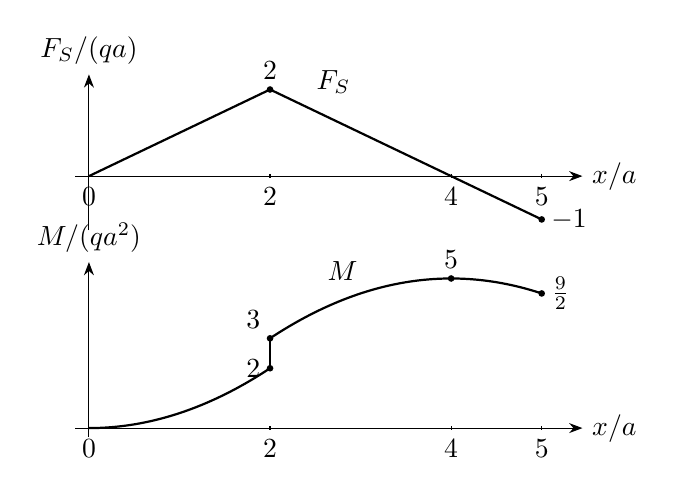
\begin{tikzpicture}[x=1.15cm,y=0.55cm,>=Stealth]
    \begin{scope}
        \draw[->] (-0.15,0) -- (5.45,0) node[right] {$x/a$};
        \draw[->] (0,-1.25) -- (0,2.35) node[above] {$F_S/(qa)$};
        \foreach \x/\lab in {0/0,2/2,4/4,5/5}{
            \draw (\x,0.05)--(\x,-0.05) node[below] {$\lab$};
        }
        \draw[thick] (0,0)--(2,2)--(5,-1);
        \fill (2,2) circle (1.2pt) node[above] {$2$};
        \fill (5,-1) circle (1.2pt) node[right] {$-1$};
        \node at (2.7,2.18) {$F_S$};
    \end{scope}
    \begin{scope}[yshift=-3.2cm,y=0.38cm]
        \draw[->] (-0.15,0) -- (5.45,0) node[right] {$x/a$};
        \draw[->] (0,-0.3) -- (0,5.55) node[above] {$M/(qa^2)$};
        \foreach \x/\lab in {0/0,2/2,4/4,5/5}{
            \draw (\x,0.06)--(\x,-0.06) node[below] {$\lab$};
        }
        \draw[thick,domain=0:2,samples=60] plot (\x,{0.5*\x*\x});
        \draw[thick] (2,2)--(2,3);
        \draw[thick,domain=2:5,samples=80] plot (\x,{-0.5*\x*\x+4*\x-3});
        \fill (2,2) circle (1.2pt) node[left] {$2$};
        \fill (2,3) circle (1.2pt) node[above left] {$3$};
        \fill (4,5) circle (1.2pt) node[above] {$5$};
        \fill (5,4.5) circle (1.2pt) node[right] {$\frac92$};
        \node at (2.8,5.25) {$M$};
    \end{scope}
\end{tikzpicture}
\end{center}

\subsection*{3. 辅助梁最小跨度}

\textbf{题图：}
\begin{center}
\includegraphics[width=0.70\linewidth]{\assetdir/q-137.png}
\end{center}

载荷直接作用于 AB 中点时
\[
    M_{\max}^{(0)}=\frac{Fl}{4},\qquad
    \frac{M_{\max}^{(0)}}{W}=1.3[\sigma].
\]
加设辅助梁后，设 $AC=DB=x$，$CD=a=l-2x$。主梁最大弯矩
\[
    M_{\max}^{(1)}=\frac{F}{2}x,
    \qquad
    \frac{M_{\max}^{(1)}}{W}=[\sigma].
\]
两式相除：
\[
    \frac{Fx/(2W)}{Fl/(4W)}=\frac{1}{1.3}
    \Rightarrow
    x=\frac{l}{2.6}.
\]
代入 $l=6\text{ m}$：
\[
    x=2.31\text{ m},\qquad
    a=l-2x=1.38\text{ m}.
\]

\subsection*{4. 齿轮轴弯扭组合强度校核}

\textbf{题图：}
\begin{center}
\includegraphics[width=0.70\linewidth]{\assetdir/q-138.png}
\end{center}

齿轮位于两支承中点。两个互相垂直方向的弯矩为
\[
    M_F=\frac{Fl}{4}
    =\frac{0.8\times10^3\times160}{4}
    =3.20\times10^4\text{ N}\cdot\text{mm},
\]
\[
    M_{F_T}=\frac{F_Tl}{4}
    =\frac{2.0\times10^3\times160}{4}
    =8.00\times10^4\text{ N}\cdot\text{mm}.
\]
合成弯矩
\[
    M=\sqrt{M_F^2+M_{F_T}^2}.
\]
扭矩为
\[
    M_T=F_T\frac{D}{2}
    =2.0\times10^3\times60
    =1.20\times10^5\text{ N}\cdot\text{mm}.
\]
实心圆轴抗弯截面系数
\[
    W=\frac{\pi d^3}{32}.
\]
第三强度理论等效应力
\[
    \sigma_{r3}
    =\frac{\sqrt{M^2+M_T^2}}{W}
    =55.7\text{ MPa}<[\sigma]=80\text{ MPa}.
\]
故该轴强度安全。


}

\chapter{2009 材料力学模拟试卷及答案六套题补充解答}
{



\section*{题源核查说明}

以下为 `2009材料力学模拟试卷及答案六套题.pdf` 中两道可由题源确认的独立补充题解。

\section*{D 卷计算题 4：应变片测力与梁强度校核}

\textbf{题意}：图示梁在 C 点贴电阻片，测得 $\varepsilon_C=0.6\times 10^{-3}$，材料弹性模量 $E=200\text{ GPa}$，许用应力 $[\sigma]=160\text{ MPa}$。求外力 $F$；若 $F=3.5\text{ kN}$，校核该梁强度。

\textbf{解}：

由应变片读数得到 C 点正应力
\[
\sigma_C=E\varepsilon_C
=200\times10^3\text{ MPa}\times0.6\times10^{-3}
=120\text{ MPa}.
\]

题图截面为矩形，取宽 $b=20\text{ mm}$、高 $h=40\text{ mm}$，抗弯截面系数为
\[
W=\frac{bh^2}{6}
=\frac{20\times40^2}{6}
=5.333\times10^3\text{ mm}^3.
\]

故 C 截面弯矩为
\[
M_C=\sigma_C W
=120\times5.333\times10^3
=6.40\times10^5\text{ N}\cdot\text{mm}
=0.640\text{ kN}\cdot\text{m}.
\]

由题图几何，C 截面对外力 $F$ 的弯矩臂为 $0.20\text{ m}$，因此
\[
M_C=0.20F
\quad\Rightarrow\quad
F=\frac{0.640}{0.20}=3.2\text{ kN}.
\]

当 $F=3.5\text{ kN}$ 时，危险截面 D 的弯矩按题图几何为
\[
M_D=0.24F=0.24\times3.5=0.84\text{ kN}\cdot\text{m}
=8.40\times10^5\text{ N}\cdot\text{mm}.
\]
于是
\[
\sigma_D=\frac{M_D}{W}
=\frac{8.40\times10^5}{5.333\times10^3}
=157.5\text{ MPa}<[\sigma]=160\text{ MPa}.
\]

所以，当 $F=3.5\text{ kN}$ 时，该梁强度满足要求。

\section*{F 卷计算题 3：辅助梁最小跨度}

\textbf{题意}：当载荷 $F$ 直接作用在简支梁 AB 中点时，梁内最大正应力超过许用应力 $30\%$。为消除这一过载现象，在中部配置辅助梁 CD。已知 $l=6\text{ m}$，求辅助梁最小跨度 $a$。

\textbf{解}：

原梁 AB 为简支梁，中点直接受集中力 $F$ 时
\[
M_{\max}^{(0)}=\frac{Fl}{4}.
\]
题意说此时最大应力超过许用应力 $30\%$，即
\[
\frac{M_{\max}^{(0)}}{W}
=\frac{Fl}{4W}
=1.3[\sigma].
\]

加设辅助梁后，集中力 $F$ 由辅助梁两端 C、D 传给主梁，主梁在 C、D 两点各受 $F/2$。设
\[
x=AC=DB,
\qquad
a=CD=l-2x.
\]
主梁最大弯矩为
\[
M_{\max}^{(1)}=\frac{F}{2}x.
\]
为刚好不超过许用应力，应满足
\[
\frac{M_{\max}^{(1)}}{W}
=\frac{Fx}{2W}
=[\sigma].
\]

两式相除得
\[
\frac{Fx/(2W)}{Fl/(4W)}
=\frac{1}{1.3}
\quad\Rightarrow\quad
\frac{2x}{l}=\frac{1}{1.3}
\quad\Rightarrow\quad
x=\frac{l}{2.6}.
\]

代入 $l=6\text{ m}$：
\[
x=\frac{6}{2.6}=2.31\text{ m},
\qquad
a=l-2x=6-2\times2.31=1.38\text{ m}.
\]

故辅助梁的最小跨度为
\[
a_{\min}=1.38\text{ m}.
\]


}

\chapter{材料力学 2009 年春季学期期中考试试题 修订解答}
{



\section*{1. 梁的内力方程与内力图 (20 分)}

\subsection*{(a) 外伸梁的内力分析 (10 分)}
\textbf{外伸梁如图 1 所示，写出内力方程，并画内力图。}

\subsubsection*{解答：}
以最左端 $A$ 为原点 $O$，以梁的轴心线为 $x$ 轴（自左向右）。
梁长为 $4a$，支座 $B$ 位于 $x=a$，支座 $C$ 位于 $x=3a$。
\noindent\textbullet\ 左端 $A$ 作用有顺时针集中力偶 $m = 2qa^2$。
\noindent\textbullet\ $BC$ 段（$a \le x \le 3a$）受向下均布载荷 $q$。
\noindent\textbullet\ 右端 $D$（$x=4a$）作用有向下集中力 $F = 2qa$。

\textbf{1. 计算支座反力}
设支座 $B$ 和 $C$ 处向上反力分别为 $R_B$ 和 $R_C$。
\noindent\textbullet\ 绕 $B$ 点力矩平衡：
  \[
  -m - (q \cdot 2a) \cdot a + R_C \cdot 2a - F \cdot 3a = 0
  \]
  将 $m = 2qa^2$，$F = 2qa$ 代入：
  \[
  -2qa^2 - 2qa^2 + R_C \cdot 2a - 6qa^2 = 0 \implies R_C = 5qa \quad (\text{向上})
  \]
\noindent\textbullet\ 竖向受力平衡：
  \[
  R_B + R_C - 2qa - F = 0 \implies R_B + 5qa - 2qa - 2qa = 0 \implies R_B = -qa \quad (\text{向下})
  \]

\textbf{2. 分段内力方程}
\noindent\textbullet\ \textbf{$AB$ 段 ($0 < x < a$)}：
  \[
  F_Q(x) = 0, \quad M(x) = 2qa^2
  \]
\noindent\textbullet\ \textbf{$BC$ 段 ($a < x < 3a$)}：
  \[
  F_Q(x) = R_B - q(x-a) = -qx
  \]
  \[
  M(x) = 2qa^2 + R_B(x-a) - \frac{1}{2}q(x-a)^2 = -\frac{1}{2}qx^2 + \frac{5}{2}qa^2
  \]
  在 $x=a$ 处，$M(a) = 2qa^2$；在 $x=3a$ 处，$M(3a) = -2qa^2$。由于 $F_Q(x) < 0$，弯矩单调递减。
\noindent\textbullet\ \textbf{$CD$ 段 ($3a < x < 4a$)}：
  \[
  F_Q(x) = R_B + R_C - 2qa = -qa + 5qa - 2qa = 2qa
  \]
  \[
  M(x) = 2qa(x-4a)
  \]
  在 $x=3a$ 处，$M(3a) = -2qa^2$；在 $x=4a$ 处，$M(4a) = 0$。

\textbf{3. 内力图特征}
\noindent\textbullet\ 剪力图：$AB$ 段为 0，$BC$ 段为斜率 $-q$ 的斜直线，$CD$ 段为常数 $2qa$。
\noindent\textbullet\ 弯矩图：$AB$ 段为常数 $2qa^2$，$BC$ 段为开口向下的二次抛物线，$CD$ 段为斜率为 $2qa$ 的斜直线。

\begin{figure}[H]
\centering
\begin{tikzpicture}[x=1.45cm,y=0.62cm,>=Latex]
  \draw[->] (-0.15,0) -- (4.35,0) node[right] {$x/a$};
  \draw[->] (0,-3.4) -- (0,2.7) node[above] {$F_Q/(qa)$};
  \foreach \x/\lab in {0/A,1/B,3/C,4/D}{
    \draw[densely dashed,gray] (\x,-3.2) -- (\x,2.35);
    \node[below] at (\x,-3.25) {$\lab$};
  }
  \draw[very thick,blue] (0,0)--(1,0);
  \draw[very thick,blue] (1,-1)--(3,-3);
  \draw[very thick,blue] (3,2)--(4,2);
  \draw[very thick,blue] (1,0)--(1,-1);
  \draw[very thick,blue] (3,-3)--(3,2);
  \draw[very thick,blue] (4,2)--(4,0);
  \node[left] at (0,0) {$0$};
  \node[right] at (1,-1) {$-1$};
  \node[right] at (3,-3) {$-3$};
  \node[above] at (3.5,2) {$2$};

  \begin{scope}[yshift=-7.4cm]
    \draw[->] (-0.15,0) -- (4.35,0) node[right] {$x/a$};
    \draw[->] (0,-2.6) -- (0,2.8) node[above] {$M/(qa^2)$};
    \foreach \x/\lab in {0/A,1/B,3/C,4/D}{
      \draw[densely dashed,gray] (\x,-2.3) -- (\x,2.45);
      \node[below] at (\x,-2.35) {$\lab$};
    }
    \draw[very thick,red] (0,2)--(1,2);
    \draw[very thick,red,domain=1:3,samples=80] plot (\x,{-0.5*\x*\x+2.5});
    \draw[very thick,red] (3,-2)--(4,0);
    \node[left] at (0,2) {$2$};
    \node[right] at (3,-2) {$-2$};
    \node[above] at (4,0) {$0$};
    \node[below] at ({sqrt(5)},0) {$\sqrt5$};
    \draw[densely dashed] ({sqrt(5)},0.1)--({sqrt(5)},-0.25);
  \end{scope}
\end{tikzpicture}
\caption{题 1(a) 剪力图和弯矩图}
\end{figure}

\subsection*{(b) 组合梁的内力分析 (10 分)}
\textbf{梁 AB 和梁 AC 在 B 点由铰链连接，载荷及几何尺寸如图 2 所示，求该梁的内力方程，并画出剪力图和弯矩图。}

\subsubsection*{解答：}
该梁为简支伸臂梁和悬臂梁组成的复合梁。以 $A$ 端固定端为原点 $O$。
梁全长为 $5a$，铰链 $B$ 位于 $x=3a$，支座 $C$ 位于 $x=5a$。
\noindent\textbullet\ $AD$ 段（$0 \le x \le a$）受均布向下载荷 $q$。
\noindent\textbullet\ $E$ 点（$x=2a$）受逆时针力偶 $m$。
\noindent\textbullet\ $F$ 点（$x=4a$）受向下集中力 $F$。

\textbf{1. 计算支座反力}
首先分析右段 $BC$（$3a \le x \le 5a$），$B$ 为铰链，$C$ 为支座。
\noindent\textbullet\ 绕 $B$ 点力矩平衡：
  \[
  R_C \cdot 2a - F \cdot a = 0 \implies R_C = \frac{F}{2} \quad (\text{向上})
  \]
\noindent\textbullet\ 竖向受力平衡，求得铰 $B$ 处剪力（左段对右段作用力）：
  \[
  V_B = F - R_C = \frac{F}{2} \quad (\text{向上})
  \]
  根据作用力与反作用力，右段对左段 $AB$ 的作用力为 $V_B = \frac{F}{2}$（向下）。

分析左段 $AB$（$0 \le x \le 3a$），固定端 $A$ 处的反力为：
\noindent\textbullet\ $R_A = qa + V_B = qa + \frac{F}{2}$
\noindent\textbullet\ $M_A = \frac{1}{2}qa^2 - m + V_B \cdot 3a = \frac{1}{2}qa^2 - m + \frac{3}{2}Fa$

\textbf{2. 分段内力方程}
\noindent\textbullet\ \textbf{$AD$ 段 ($0 < x < a$)}：
  \[
  F_Q(x) = R_A - qx = qa + \frac{F}{2} - qx
  \]
  \[
  M(x) = -M_A + R_A x - \frac{1}{2}qx^2 = -\left(\frac{1}{2}qa^2 - m + \frac{3}{2}Fa\right) + \left(qa + \frac{F}{2}\right)x - \frac{1}{2}qx^2
  \]
\noindent\textbullet\ \textbf{$DE$ 段 ($a < x < 2a$)}：
  \[
  F_Q(x) = \frac{F}{2}, \quad M(x) = m - \frac{3}{2}Fa + \frac{F}{2}x
  \]
\noindent\textbullet\ \textbf{$EB$ 段 ($2a < x < 3a$)}：
  由于 $x=2a$ 处有逆时针力偶 $m$，弯矩图有突变：
  \[
  F_Q(x) = \frac{F}{2}, \quad M(x) = -\frac{3}{2}Fa + \frac{F}{2}x
  \]
  在 $x=3a$ 处，$M(3a) = 0$（符合铰链处弯矩为 0 的物理实际）。
\noindent\textbullet\ \textbf{$BF$ 段 ($3a < x < 4a$)}：
  \[
  F_Q(x) = \frac{F}{2}, \quad M(x) = -\frac{3}{2}Fa + \frac{F}{2}x
  \]
\noindent\textbullet\ \textbf{$FC$ 段 ($4a < x < 5a$)}：
  \[
  F_Q(x) = -\frac{F}{2}, \quad M(x) = R_C(5a-x) = \frac{F}{2}(5a-x)
  \]

\textbf{3. 内力图}

\begin{figure}[H]
\centering
\begin{tikzpicture}[x=1.25cm,y=0.72cm,>=Latex]
  \draw[->] (-0.15,0) -- (5.35,0) node[right] {$x/a$};
  \draw[->] (0,-2.1) -- (0,3.0) node[above] {$F_Q$};
  \foreach \x/\lab in {0/A,1/D,2/E,3/B,4/F,5/C}{
    \draw[densely dashed,gray] (\x,-1.8) -- (\x,2.65);
    \node[below] at (\x,-1.85) {$\lab$};
  }
  \draw[very thick,blue] (0,2.3)--(1,1.1);
  \draw[very thick,blue] (1,1.1)--(4,1.1);
  \draw[very thick,blue] (4,1.1)--(4,-1.1);
  \draw[very thick,blue] (4,-1.1)--(5,-1.1);
  \draw[very thick,blue] (5,-1.1)--(5,0);
  \node[left] at (0,2.3) {$qa+\frac F2$};
  \node[above] at (2.7,1.1) {$\frac F2$};
  \node[below] at (4.5,-1.1) {$-\frac F2$};

  \begin{scope}[yshift=-7.1cm]
    \draw[->] (-0.15,0) -- (5.35,0) node[right] {$x/a$};
    \draw[->] (0,-2.4) -- (0,2.8) node[above] {$M$};
    \foreach \x/\lab in {0/A,1/D,2/E,3/B,4/F,5/C}{
      \draw[densely dashed,gray] (\x,-2.1) -- (\x,2.45);
      \node[below] at (\x,-2.15) {$\lab$};
    }
    \draw[very thick,red] (0,-0.7) .. controls (0.45,0.35) and (0.75,1.0) .. (1,1.2);
    \draw[very thick,red] (1,1.2)--(2,1.7);
    \draw[very thick,red] (2,1.7)--(2,-0.9);
    \draw[very thick,red] (2,-0.9)--(3,0);
    \draw[very thick,red] (3,0)--(4,0.9);
    \draw[very thick,red] (4,0.9)--(5,0);
    \node[left] at (0,-0.7) {$m-\frac12qa^2-\frac32Fa$};
    \node[above] at (1,1.2) {$m-Fa$};
    \node[above] at (2,1.7) {$m-\frac12Fa$};
    \node[right] at (2,-0.9) {$-\frac12Fa$};
    \node[above] at (4,0.9) {$\frac12Fa$};
    \node[above] at (3,0) {$0$};
  \end{scope}
\end{tikzpicture}
\caption{题 1(b) 剪力图和弯矩图（纵向按符号表达式标注）}
\end{figure}


% \newpage removed


\section*{2. 偏心拉弯组合柱的强度与中性轴 (20 分)}

\textbf{矩形截面如图 3 所示，已知 $q=2\text{ kN/m}$，$P_0=240\text{ kN}$，$P_1=160\text{ kN}$，$P_2=4\text{ kN}$，$b=12\text{ cm}$，$l=2\text{ m}$，$h=16\text{ cm}$。求梁内的最大拉应力和压应力以及危险截面上中性轴的位置。}

\subsubsection*{解答：}

建立坐标系：以柱顶轴心为原点，纵向轴为 $x$ 轴（向下），$y$ 轴指向左侧，$z$ 轴指向纸面向里。
\noindent\textbullet\ 截面面积：$A = b \cdot h = 0.12\text{ m} \times 0.16\text{ m} = 0.0192\text{ m}^2$。
\noindent\textbullet\ 惯性矩：
\[
I_z = \frac{bh^3}{12} = 4.096 \times 10^{-5}\text{ m}^4,\qquad
I_y = \frac{hb^3}{12} = 2.304 \times 10^{-5}\text{ m}^4.
\]

\textbf{1. 内力分析}
在任意截面 $x$（自顶端向下， $0 \le x \le 2\text{ m}$）：
\noindent\textbullet\ 轴力恒为常数：
  \[
  N_x = -(P_0 + P_1) = -(240 + 160) = -400\text{ kN} \quad (\text{压})
  \]
\noindent\textbullet\ 弯矩 $M_z(x)$（使 $y > 0$ 侧受拉为正）：
\noindent\textbullet\ $P_1$ 偏心距为 $e_y = -h/2 = -0.08\text{ m}$，产生恒定弯矩：
    \[
    M_{z, P_1} = -P_1 \cdot e_y = 160\text{ kN} \times 0.08\text{ m} = 12.8\text{ kN}\cdot\text{m}
    \]
\noindent\textbullet\ 均布载荷 $q = 2\text{ kN/m}$ 产生弯矩：
    \[
    M_{z, q}(x) = -\frac{1}{2} q x^2 = -x^2 \quad (\text{kN}\cdot\text{m})
    \]
\noindent\textbullet\ 集中力 $P_2 = 4\text{ kN}$ 位于 $x=l/2=1\text{ m}$ 处，按图沿 $z$ 轴反向作用，因此它不进入 $M_z$，而产生绕 $y$ 轴的弯矩
\[
M_y(x)=
\begin{cases}
0, & 0\le x<1,\\
-P_2(x-1)=-4(x-1), & 1<x\le 2
\end{cases}
\quad(\text{kN}\cdot\text{m}).
\]

因此，分段弯矩方程为：
\noindent\textbullet\ $0 \le x < 1$ 时：
  \[
  M_z(x) = 12.8 - x^2
  \]
  此段弯矩单调递减，端点值为 $M_z(0) = 12.8\text{ kN}\cdot\text{m}$，$M_z(1^-) = 11.8\text{ kN}\cdot\text{m}$。
\noindent\textbullet\ $1 < x \le 2$ 时：
  \[
  M_z(x) = 12.8 - x^2
  \]
  此段继续单调递减，端点值为 $M_z(1^+) = 11.8\text{ kN}\cdot\text{m}$，$M_z(2) = 8.8\text{ kN}\cdot\text{m}$；同时 $|M_y(2)|=4.0\text{ kN}\cdot\text{m}$。

因此需比较顶端截面 $x=0$ 与底端固定截面 $x=2\text{ m}$。顶端只有 $M_z=12.8\text{ kN}\cdot\text{m}$；底端同时有 $M_z=8.8\text{ kN}\cdot\text{m}$ 与 $M_y=-4.0\text{ kN}\cdot\text{m}$。

\textbf{2. 危险截面上的正应力计算}
偏心压弯组合下，截面任一点的正应力为
\[
\sigma_x = \frac{N_x}{A}+\frac{M_z y}{I_z}-\frac{M_y z}{I_y}.
\]
其中 $y=\pm h/2=\pm0.08\text{ m}$，$z=\pm b/2=\pm0.06\text{ m}$。

顶端截面 $x=0$：
\[
\sigma_x=-20.833+312.5y\quad(\text{MPa},\ y\text{ 以 m 计}),
\]
故该截面最大拉、压应力分别为 $4.167\text{ MPa}$ 与 $-45.833\text{ MPa}$。

底端截面 $x=2\text{ m}$：
\[
\sigma_x=-20.833+214.844y+173.611z\quad(\text{MPa},\ y,z\text{ 以 m 计}).
\]
代入四个角点比较：
\[
\begin{array}{c|c|c|c}
y(\text{m}) & z(\text{m}) & \sigma_x(\text{MPa}) & \text{性质}\\
\hline
0.08 & 0.06 & 6.771 & \text{拉}\\
0.08 & -0.06 & -14.062 & \text{压}\\
-0.08 & 0.06 & -27.604 & \text{压}\\
-0.08 & -0.06 & -48.438 & \text{压}
\end{array}
\]

因此全柱最大拉应力为 $6.77\text{ MPa}$，最大压应力为 $48.44\text{ MPa}$，均发生在底端固定截面；若采用相反的 $z$ 轴正向，两个 $z$ 边角互换，但数值不变。

\textbf{3. 中性轴位置}
危险截面为底端截面，令 $\sigma_x=0$，中性轴方程为
\[
-20.833+214.844y+173.611z=0\quad(y,z\text{ 以 m 计}).
\]
它在边 $y=0.08\text{ m}$ 上交于 $z=0.0210\text{ m}=2.10\text{ cm}$，在边 $z=0.06\text{ m}$ 上交于 $y=0.0485\text{ m}=4.85\text{ cm}$。


% \newpage removed


\section*{3. 层叠梁与胶合梁的正应力对比 (20 分)}

\textbf{如图 4 所示，材料相同、宽度相等、厚度比 $h_1 / h_2 = 1/2$ 的两块板，组成一简支梁，其上承受均布载荷 $q$。
(1) 若两块板只是互相重叠在一起，求此时两块板内的最大正应力之比；
(2) 若两块板胶合在一起，不互相滑动，问此时的最大正应力比前一种情况减少了多少？}

\subsubsection*{解答：}

\textbf{1. 两块板叠合在一起（无摩擦滑动）}
由于两板材料相同，弯曲变形时曲率 $\chi$ 相同：
\[
\chi = \frac{M_1}{EI_1} = \frac{M_2}{EI_2} \implies \frac{M_1}{M_2} = \frac{I_1}{I_2} = \left(\frac{h_1}{h_2}\right)^3 = \left(\frac{1}{2}\right)^3 = \frac{1}{8}
\]
两块板分别独立承受弯曲正应力，其最大正应力分别为：
\[
\sigma_{1,\max} = \frac{M_1}{W_1} = \frac{M_1}{\frac{b h_1^2}{6}}, \quad \sigma_{2,\max} = \frac{M_2}{W_2} = \frac{M_2}{\frac{b h_2^2}{6}}
\]
两者之比为：
\[
\frac{\sigma_{1,\max}}{\sigma_{2,\max}} = \frac{M_1}{M_2} \left(\frac{h_2}{h_1}\right)^2 = \frac{1}{8} \times 4 = \frac{1}{2}
\]
此时梁内的最大正应力为下板的最大正应力：
\[
\sigma_{\max, \mathrm{s}} = \sigma_{2,\max} = \frac{M_2}{W_2} = \frac{\frac{8}{9}M}{\frac{b h_2^2}{6}} = \frac{16M}{3b h_2^2}
\]

\textbf{2. 两块板胶合在一起（形成一体）}
胶合后成为一整体矩形截面，宽度为 $b$，总高度为 $h = h_1 + h_2 = 1.5 h_2$。
最大正应力发生在梁的外侧边缘：
\[
\sigma_{\max, \mathrm{b}} = \frac{M}{W} = \frac{M}{\frac{bh^2}{6}} = \frac{6M}{b (1.5 h_2)^2} = \frac{8M}{3b h_2^2}
\]

最大正应力比前一种情况减少了：
\[
\eta = \frac{\sigma_{\max, \mathrm{s}} - \sigma_{\max, \mathrm{b}}}{\sigma_{\max, \mathrm{s}}} = \frac{\frac{16M}{3b h_2^2} - \frac{8M}{3b h_2^2}}{\frac{16M}{3b h_2^2}} = 50\%
\]


% \newpage removed


\section*{4. 薄壁圆环扭转剪应力公式推导 (20 分)}

\textbf{试推导薄壁圆环受扭矩 $M$ 时的切应力公式。}

\subsubsection*{解答：}

设薄壁圆环的平均半径为 $R$，壁厚为 $t$（且满足 $t \ll R$）。

\textbf{1. 几何与变形协调条件}
由于圆环截面具有轴对称性，扭转时满足平面假设。各横截面绕轴线旋转，且半径线仍保持为直线。
在半径 $r$ 处，圆环的剪应变 $\gamma$ 与扭转角变化率 $\theta'$（单位长度扭转角）的关系为：
\[
\gamma(r) = r \theta'
\]

\textbf{2. 物理关系（剪切胡克定律）}
由剪切胡克定律，半径 $r$ 处的剪应力 $\tau(r)$ 为：
\[
\tau(r) = G \gamma(r) = G \theta' r
\]

\textbf{3. 静力平衡条件}
横截面上的扭矩 $M$ 应等于横截面上各微面积上的剪应力对圆心矩之和：
\[
M = \int_A \tau(r) r \diff A = G \theta' \int_A r^2 \diff A = G \theta' I_p
\]
其中 $I_p$ 为极惯性矩：
\[
I_p = \int_A r^2 \diff A
\]
由于壁厚极薄 ($t \ll R$)，可认为极惯性矩近似为：
\[
I_p \approx A R^2 = (2\pi R t) R^2 = 2\pi R^3 t
\]
亦可由积分精确求得：
\[
I_p = \frac{\pi}{2} \left[ \left(R+\frac{t}{2}\right)^4 - \left(R-\frac{t}{2}\right)^4 \right] \approx 2\pi R^3 t
\]

\textbf{4. 剪应力公式}
因为壁厚 $t$ 极小，横截面上的剪应力沿壁厚方向可视为均匀分布，且等于平均半径处的剪应力：
\[
\tau \approx \frac{M R}{I_p} = \frac{M R}{2\pi R^3 t} = \frac{M}{2\pi R^2 t}
\]


% \newpage removed


\section*{5. 不对称薄壁 I 形梁剪切流动与弯曲中心 (20 分)}

\textbf{不对称工字型截面悬臂梁受力以及横截面上的剪力方向如图 6 所示。请分析：\\
(1) 横截面的腹板上的任意点处是否存在水平方向的切应力；\\
(2) 翼缘的切应力流的方向；\\
(3) 判断弯曲中心的大致位置。}

\subsubsection*{解答：}

取腹板中线为水平对称轴。按图示横截面剪力方向记为向下。薄壁截面剪应力流沿截面壁的切线方向流动，因此翼缘内的剪力流沿竖直方向；腹板为水平壁，若有剪力流则沿水平方向。

\begin{enumerate}[label=(\arabic*)]
  \item \textbf{腹板上是否有水平方向切应力}

  本截面关于水平腹板中线对称。对任一竖直翼缘，由于其上、下自由边处剪力流均为零，剪力流从自由边向腹板中线逐渐增大，并在腹板连接处连续通过；上、下两半翼缘在连接点处的流量相等、方向相接，流入水平腹板分支的净剪力流为零。

  因此，水平腹板内的剪力流为零。按薄壁剪力流模型，腹板上任意点不存在水平方向切应力。

  \item \textbf{翼缘剪应力流方向}

  左、右翼缘中的剪力流均沿翼缘竖向分布。按图示截面剪力向下，两个翼缘内的剪力流方向均为向下。剪力流在各翼缘的上、下自由边为零，在腹板中线附近达到最大值。若截面剪力方向反取，则上述箭向全部反向。

  \item \textbf{弯曲中心的大致位置}

  由于截面关于腹板中线对称，弯曲中心必在该水平对称轴上。腹板不提供水平剪力流，竖向剪力主要由两竖直翼缘承担。

  设左、右翼缘承担的竖向剪力合力分别为 $V_1,V_2$，两翼缘剪力合力作用线间距为 $d$。同厚薄壁竖直翼缘中，剪力合力与翼缘高度的三次方成正比，故
  \[
  \frac{V_1}{V_2}
  =
  \left(\frac{5h}{10h}\right)^3
  =
  \frac{1}{8},
  \qquad
  V_2=8V_1 .
  \]
  弯曲中心即剪力流合力的作用点，故其到左翼缘剪力合力作用线的距离为
  \[
  e=\frac{V_2}{V_1+V_2}d=\frac{8}{9}d.
  \]
  因此，弯曲中心位于腹板中线上、两翼缘之间，并明显靠近右侧较高翼缘。

  若将图中两翼缘间距近似取为 $d\simeq 5h$，则
  \[
  e\simeq \frac{40}{9}h,
  \]
  即距右翼缘约 $5h/9$。若按翼缘中线距离计，数值随 $d$ 相应调整，但“靠近右翼缘”的判断不变。
\end{enumerate}


}

\chapter{清华大学 2010 年《材料力学》期终测验试卷 (A卷) 修订解答}
{


\vspace{-1.0cm}

\section*{一、选择题（每小题 5 分，共 20 分）}

\textbf{（1）悬臂梁受集中力和集中力偶作用，相应的弯矩图如图所示。由此可以确定梁上的载荷 $F$、$m$ 的值分别为：}

\begin{minipage}{0.48\textwidth}
\textbf{（A）$F = 6\text{ kN}$， $m = 10\text{ kNm}$} \\
\textbf{（B）$F = 6\text{ kN}$， $m = 6\text{ kNm}$} \\
\textbf{（C）$F = 4\text{ kN}$， $m = 4\text{ kNm}$} \\
\textbf{（D）$F = 4\text{ kN}$， $m = 6\text{ kNm}$}
\end{minipage}
\begin{minipage}{0.5\textwidth}
\centering
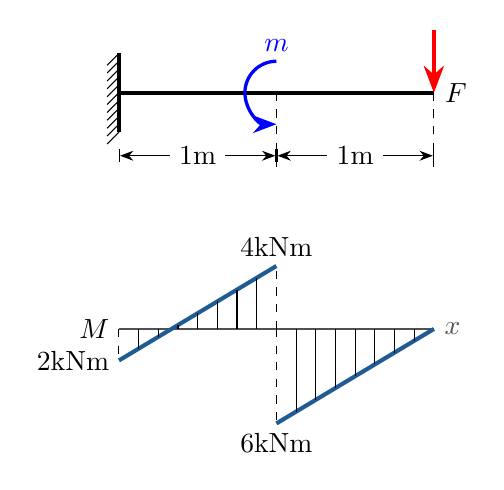
\begin{tikzpicture}[scale=1.0, >=Stealth]
    % Draw beam
    \draw [line width=1.5pt] (0,0.8) -- (4,0.8);
    % Fixed support
    \draw [line width=1.5pt] (0,0.3) -- (0,1.3);
    \foreach \y in {0.3, 0.4, 0.5, 0.6, 0.7, 0.8, 0.9, 1.0, 1.1, 1.2, 1.3}
        \draw (0,\y) -- (-0.15,\y-0.15);
    
    % Force F
    \draw [->, line width=1.5pt, red] (4,1.6) -- (4,0.8) node[right, black] {$F$};
    
    % Moment m at middle
    \draw [->, line width=1.2pt, blue] (2,1.2) arc (90:270:0.4);
    \node [above, blue] at (2,1.2) {$m$};
    
    % Dimension
    \draw [|<->|] (0,0) -- (2,0) node[midway, fill=white] {$1\text{m}$};
    \draw [|<->|] (2,0) -- (4,0) node[midway, fill=white] {$1\text{m}$};
    \draw [dashed] (2,0.8) -- (2,-0.2);
    \draw [dashed] (4,0.8) -- (4,-0.2);
    
    % Bending Moment Diagram
    \begin{scope}[yshift=-2.2cm]
        \draw [line width=1.0pt, axisgray] (0,0) -- (4,0) node[right] {$x$};
        \node [left] at (0,0) {$M$};
        
        % Right segment (0 to 6)
        \draw [line width=1.5pt, accent] (4,0) -- (2,-1.2);
        \draw [dashed] (2,0) -- (2,-1.2) node[below] {$6\text{kNm}$};
        \foreach \x in {2.25, 2.5, 2.75, 3.0, 3.25, 3.5, 3.75}
            \draw (\x,0) -- (\x, -1.2 + 0.6* \x - 1.2);
            
        % Left segment (4 to -2)
        \draw [line width=1.5pt, accent] (2,0.8) -- (0,-0.4);
        \draw [dashed] (2,0) -- (2,0.8) node[above] {$4\text{kNm}$};
        \draw [dashed] (0,0) -- (0,-0.4) node[left] {$2\text{kNm}$};
        \foreach \x in {0.25, 0.5, 0.75, 1.0, 1.25, 1.5, 1.75}
            \draw (\x,0) -- (\x, -0.4 + 0.6*\x);
    \end{scope}
\end{tikzpicture}
\end{minipage}

\subsubsection*{解答：选（A）}
1. \textbf{确定集中力 $F$}：
   在梁的右半段 $x \in (1\text{ m}, 2\text{ m})$，只受自由端的集中力 $F$ 作用，其剪力 $V = F$（常数）。根据弯矩与剪力的微分关系：
   \[
       \frac{\diff M}{\diff x} = V = F
   \]
   由此可知弯矩图斜率为 $F$。由于中点处弯矩值为 $6\text{ kNm}$，自由端弯矩为 0，长度为 $1\text{ m}$，所以斜率大小为：
   \[
       F = \frac{\Delta M}{\Delta x} = \frac{6\text{ kNm} - 0}{1\text{ m}} = 6\text{ kN}
   \]
2. \textbf{确定集中力偶 $m$}：
   在中点 $x = 1\text{ m}$ 处，外加集中力偶 $m$ 导致弯矩图发生突变。突变量的大小等于集中力偶的数值：
   \[
       m = |M(1^+) - M(1^-)| = | (-6\text{ kNm}) - 4\text{ kNm} | = 10\text{ kNm}
   \]
   （由于力偶为逆时针方向，截面弯矩从负弯矩向正弯矩方向突变，突变量为 $10\text{ kNm}$，符合图示）。
   
因此，正确答案为 \textbf{A}。


% \newpage removed


\textbf{（2）按照第三强度理论，判断在图示两种应力状态中危险程度是：}

\begin{minipage}{0.45\textwidth}
\textbf{（A）（a）更危险} \\
\textbf{（B）（b）更危险} \\
\textbf{（C）两者相同} \\
\textbf{（D）无法判断}
\end{minipage}
\begin{minipage}{0.5\textwidth}
\centering
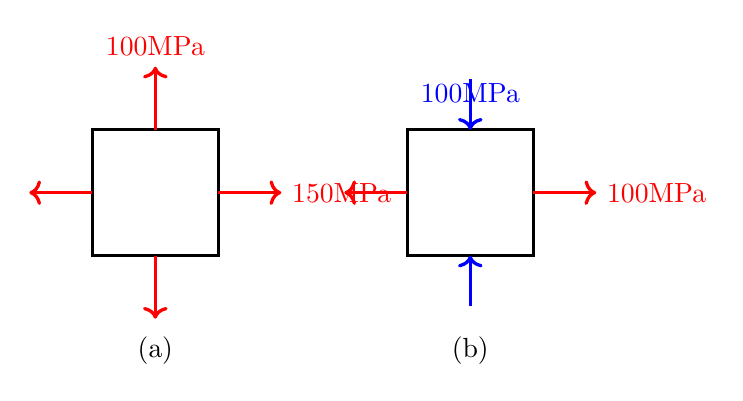
\begin{tikzpicture}[scale=0.8]
    % State (a)
    \draw [line width=1.2pt] (-1,-1) rectangle (1,1);
    \draw [->, line width=1.2pt, red] (1,0) -- (2,0) node[right] {$150\text{MPa}$};
    \draw [->, line width=1.2pt, red] (-1,0) -- (-2,0);
    \draw [->, line width=1.2pt, red] (0,1) -- (0,2) node[above] {$100\text{MPa}$};
    \draw [->, line width=1.2pt, red] (0,-1) -- (0,-2);
    \node at (0,-2.5) {(a)};
    
    % State (b)
    \begin{scope}[xshift=5.0cm]
        \draw [line width=1.2pt] (-1,-1) rectangle (1,1);
        \draw [->, line width=1.2pt, red] (1,0) -- (2,0) node[right] {$100\text{MPa}$};
        \draw [->, line width=1.2pt, red] (-1,0) -- (-2,0);
        \draw [->, line width=1.2pt, blue] (0,1.8) -- (0,1) node[above, yshift=6pt] {$100\text{MPa}$};
        \draw [->, line width=1.2pt, blue] (0,-1.8) -- (0,-1);
        
        \node at (0,-2.5) {(b)};
    \end{scope}
\end{tikzpicture}
\end{minipage}

\subsubsection*{解答：选（B）}
根据第三强度理论（Tresca 屈服准则），当量应力为：
\[
    \sigma_{r3} = \sigma_1 - \sigma_3
\]
我们需要计算两者的主应力大小：

1. \textbf{应力状态 (a)}：
   为双轴拉伸状态，剪应力为零。所以主应力直接为：
   \[
       \sigma_1 = 150\text{ MPa}, \quad \sigma_2 = 100\text{ MPa}, \quad \sigma_3 = 0
   \]
   其当量应力为：
   \[
       \sigma_{r3}^{(a)} = \sigma_1 - \sigma_3 = 150 - 0 = 150\text{ MPa}
   \]

2. \textbf{应力状态 (b)}：
   原图中 (b) 为双向一拉一压状态，没有剪应力：
   \[
       \sigma_x=100\text{ MPa},\qquad \sigma_y=-100\text{ MPa},\qquad \tau_{xy}=0.
   \]
   因此主应力为
   \[
       \sigma_1=100\text{ MPa},\qquad \sigma_2=0,\qquad \sigma_3=-100\text{ MPa}.
   \]
   其第三强度理论当量应力为
   \[
       \sigma_{r3}^{(b)}=\sigma_1-\sigma_3=100-(-100)=200\text{ MPa}.
   \]

因为 $\sigma_{r3}^{(b)} = 200\text{ MPa} > \sigma_{r3}^{(a)} = 150\text{ MPa}$，所以应力状态 (b) 更危险。


% \newpage removed


\textbf{（3）图示悬臂梁的自由端承受集中力偶 $M_e$，若梁的长度减少一半，则梁的最大挠度是原来的：}

\begin{minipage}{0.48\textwidth}
\textbf{（A）$1/2$} \\
\textbf{（B）$1/4$} \\
\textbf{（C）$1/8$} \\
\textbf{（D）$1/16$}
\end{minipage}
\begin{minipage}{0.5\textwidth}
\centering
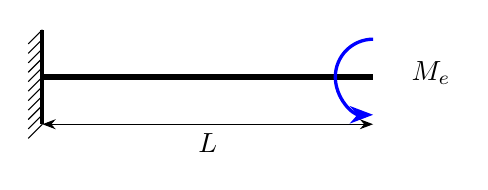
\begin{tikzpicture}[scale=1.2, >=Stealth]
    % Support
    \draw [line width=1.5pt] (0,0.3) -- (0,1.3);
    \foreach \y in {0.3, 0.4, 0.5, 0.6, 0.7, 0.8, 0.9, 1.0, 1.1, 1.2, 1.3}
        \draw (0,\y) -- (-0.15,\y-0.15);
    % Beam
    \draw [line width=2.0pt] (0,0.8) -- (3.5,0.8);
    % Moment Me
    \draw [->, line width=1.2pt, blue] (3.5, 1.2) arc (90:270:0.4) node[right, xshift=10pt, yshift=15pt, black] {$M_e$};
    % Length
    \draw [<->] (0, 0.3) -- (3.5, 0.3) node[midway, below] {$L$};
\end{tikzpicture}
\end{minipage}

\subsubsection*{解答：选（B）}
对于长度为 $L$，弯曲刚度为 $EI$ 的悬臂梁，自由端承受集中力偶 $M_e$。
梁的弯矩方程为恒值 $M(x) = M_e$。根据挠曲线近似微分方程：
\[
    EI w''(x) = M_e
\]
积分两次并代入固定端边界条件 $w(0) = 0$ 和 $w'(0) = 0$，得到挠曲线方程为：
\[
    w(x) = \frac{M_e x^2}{2EI}
\]
最大挠度发生在自由端 $x=L$ 处：
\[
    w_{\max} = \frac{M_e L^2}{2EI}
\]
由公式可见，最大挠度与梁的长度 $L$ 的平方成正比。
若梁的长度减少一半变为 $L/2$，则新的最大挠度为：
\[
    w_{\max}' = \frac{M_e (L/2)^2}{2EI} = \frac{1}{4} \left( \frac{M_e L^2}{2EI} \right) = \frac{1}{4} w_{\max}
\]
所以，最大挠度是原来的 $1/4$。


% \newpage removed


\textbf{（4）如图所示两端简支细长压杆，在材料弹性模量和横截面积相同的前提下，杆的横截面有两种选择，形状尺寸分别如图（a）、(b)所示。则图（a）截面情况对应的压杆临界力是图（b）截面情况对应压杆临界力的：}

\begin{minipage}{0.48\textwidth}
\textbf{（A）$2$} \\
\textbf{（B）$1/2$} \\
\textbf{（C）$1/4$} \\
\textbf{（D）$4$}
\end{minipage}
\begin{minipage}{0.5\textwidth}
\centering
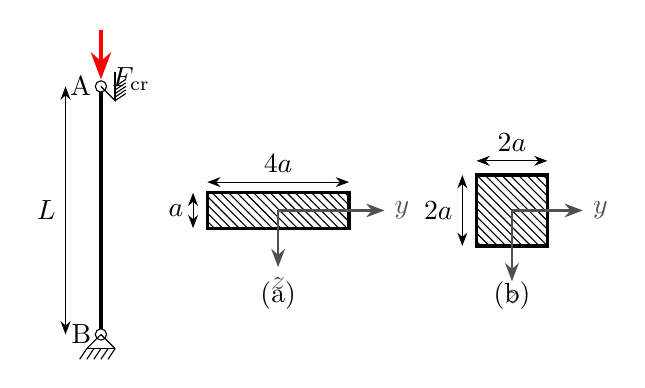
\begin{tikzpicture}[scale=0.9, >=Stealth]
    % Column
    \draw [line width=1.5pt] (0,0) -- (0,3.5);
    \draw [fill=white] (0,3.5) circle (0.08);
    \draw [fill=white] (0,0) circle (0.08);
    % Supports
    \draw (-0.2, -0.2) -- (0.2, -0.2);
    \draw (-0.2, -0.2) -- (0, 0);
    \draw (0.2, -0.2) -- (0, 0);
    \foreach \x in {-0.2, -0.1, 0, 0.1, 0.2}
        \draw (\x, -0.2) -- (\x-0.1, -0.35);
        
    \draw (0.2, 3.5) -- (0.2, 3.3) -- (0, 3.5);
    \foreach \y in {3.3, 3.35, 3.4, 3.45, 3.5}
        \draw (0.2, \y) -- (0.35, \y+0.1);
    \draw [line width=1pt] (0.2, 3.3) -- (0.2, 3.7);
    
    \draw [->, line width=1.5pt, red] (0,4.3) -- (0,3.6) node[right, black] {$F_{\text{cr}}$};
    \draw [<->] (-0.5,0) -- (-0.5,3.5) node[midway, left] {$L$};
    \node [left] at (0,3.5) {A};
    \node [left] at (0,0) {B};
    
    % Section (a)
    \begin{scope}[xshift=2.5cm, yshift=1.75cm]
        \draw [line width=1.2pt, pattern=north west lines] (-1.0, -0.25) rectangle (1.0, 0.25);
        \draw [->, line width=0.8pt, axisgray] (0,0) -- (1.5,0) node[right] {$y$};
        \draw [->, line width=0.8pt, axisgray] (0,0) -- (0,-0.8) node[below] {$z$};
        \draw [<->] (-1.0, 0.4) -- (1.0, 0.4) node[midway, above] {$4a$};
        \draw [<->] (-1.2, -0.25) -- (-1.2, 0.25) node[midway, left] {$a$};
        \node at (0,-1.2) {(a)};
    \end{scope}
    
    % Section (b)
    \begin{scope}[xshift=5.8cm, yshift=1.75cm]
        \draw [line width=1.2pt, pattern=north west lines] (-0.5, -0.5) rectangle (0.5, 0.5);
        \draw [->, line width=0.8pt, axisgray] (0,0) -- (1.0,0) node[right] {$y$};
        \draw [->, line width=0.8pt, axisgray] (0,0) -- (0,-1.0) node[below] {$z$};
        \draw [<->] (-0.5, 0.7) -- (0.5, 0.7) node[midway, above] {$2a$};
        \draw [<->] (-0.7, -0.5) -- (-0.7, 0.5) node[midway, left] {$2a$};
        \node at (0,-1.2) {(b)};
    \end{scope}
\end{tikzpicture}
\end{minipage}

\subsubsection*{解答：选（C）}
两端简支细长压杆的欧拉临界力计算公式为：
\[
    F_{\text{cr}} = \frac{\pi^2 E I_{\min}}{L^2}
\]
由于压杆在两个对称轴方向上均可发生弯曲失稳，其临界力由截面的最小惯性矩 $I_{\min}$ 决定。

1. \textbf{计算截面 (a) 的最小惯性矩}：
   截面为宽 $4a$、高 $a$ 的矩形。
   \[
       I_y^{(a)} = \frac{b h^3}{12} = \frac{4a \cdot a^3}{12} = \frac{1}{3} a^4
   \]
   \[
       I_z^{(a)} = \frac{h b^3}{12} = \frac{a \cdot (4a)^3}{12} = \frac{16}{3} a^4
   \]
   所以，截面 (a) 的最小惯性矩为：
   \[
       I_{\min}^{(a)} = I_y^{(a)} = \frac{1}{3} a^4
   \]

2. \textbf{计算截面 (b) 的最小惯性矩}：
   截面为边长 $2a$ 的正方形。
   \[
       I_{\min}^{(b)} = I_y^{(b)} = I_z^{(b)} = \frac{(2a) \cdot (2a)^3}{12} = \frac{16}{12} a^4 = \frac{4}{3} a^4
   \]

3. \textbf{计算临界力之比}：
   由于材料（$E$）和长度（$L$）完全相同，临界力之比等于最小惯性矩之比：
   \[
       \frac{F_{\text{cr}}^{(a)}}{F_{\text{cr}}^{(b)}} = \frac{I_{\min}^{(a)}}{I_{\min}^{(b)}} = \frac{\frac{1}{3} a^4}{\frac{4}{3} a^4} = \frac{1}{4}
   \]
因此，图 (a) 截面对应的临界力是图 (b) 的 $1/4$。


% \newpage removed


\section*{二、挠曲线积分求解题（20分）}

\textbf{2. 如图所示，已知：$q$、$EI$、$l$。试根据梁的挠曲线微分方程和约束条件，求梁的挠度曲线表达式，并给出梁自由端截面处的挠度和转角。}

\centering
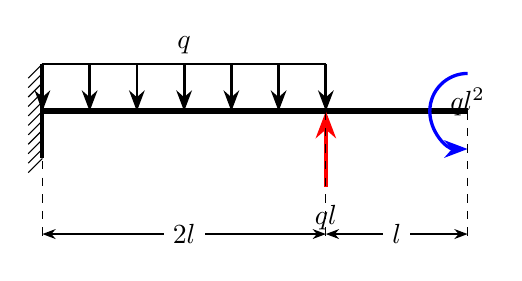
\begin{tikzpicture}[scale=1.2, >=Stealth]
    % Cantilever Fixed support
    \draw [line width=1.5pt] (0,0.5) -- (0,1.5);
    \foreach \y in {0.5, 0.6, 0.7, 0.8, 0.9, 1.0, 1.1, 1.2, 1.3, 1.4, 1.5}
        \draw (0,\y) -- (-0.15,\y-0.15);
        
    % Beam
    \draw [line width=2.0pt] (0,1.0) -- (4.5,1.0);
    
    % Distributed load q on [0, 2l] (0 to 3cm)
    \draw [line width=1.0pt, ->] (0, 1.5) -- (0, 1.0);
    \draw [line width=1.0pt, ->] (0.5, 1.5) -- (0.5, 1.0);
    \draw [line width=1.0pt, ->] (1.0, 1.5) -- (1.0, 1.0);
    \draw [line width=1.0pt, ->] (1.5, 1.5) -- (1.5, 1.0);
    \draw [line width=1.0pt, ->] (2.0, 1.5) -- (2.0, 1.0);
    \draw [line width=1.0pt, ->] (2.5, 1.5) -- (2.5, 1.0);
    \draw [line width=1.0pt, ->] (3.0, 1.5) -- (3.0, 1.0);
    \draw [line width=1.0pt] (0, 1.5) -- (3.0, 1.5);
    \node [above] at (1.5, 1.5) {$q$};
    
    % Force ql at 2l
    \draw [->, line width=1.5pt, red] (3.0, 0.2) -- (3.0, 1.0) node[below, yshift=-30pt, black] {$ql$};
    
    % Moment ql^2 at free end 3l
    \draw [->, line width=1.2pt, blue] (4.5, 1.4) arc (90:270:0.4) node[above, yshift=8pt, black] {$ql^2$};
    
    % Dimension
    \draw [dashed] (0,1.0) -- (0, -0.4);
    \draw [dashed] (3.0,1.0) -- (3.0, -0.4);
    \draw [dashed] (4.5,1.0) -- (4.5, -0.4);
    \draw [<->] (0,-0.3) -- (3.0,-0.3) node[midway, fill=white] {$2l$};
    \draw [<->] (3.0,-0.3) -- (4.5,-0.3) node[midway, fill=white] {$l$};
\end{tikzpicture}

\flushleft

\subsubsection*{解答：}

以固定端为原点，梁轴向右为 $x$ 轴正方向，挠度 $w(x)$ 向上为正。按图示力偶方向取正弯矩，梁分为 $0\le x\le2l$ 与 $2l\le x\le3l$ 两段。

\textbf{1. 弯矩方程}

从截面右侧取隔离体。对 $2l\le x\le3l$，右侧只有自由端力偶：
\[
M_2(x)=ql^2 .
\]
对 $0\le x\le2l$，右侧包含自由端力偶、$x=2l$ 处向上的集中力 $ql$，以及 $x$ 至 $2l$ 范围内向下的均布载荷：
\[
M_1(x)=ql^2+ql(2l-x)-\frac{q}{2}(2l-x)^2
=ql^2+qlx-\frac{1}{2}qx^2 .
\]

\textbf{2. 分段积分}

由 $EIw''=M$，第一段为
\[
EIw_1''=ql^2+qlx-\frac{1}{2}qx^2,
\]
\[
EIw_1'=ql^2x+\frac{1}{2}qlx^2-\frac{1}{6}qx^3+C_1,
\]
\[
EIw_1=\frac{1}{2}ql^2x^2+\frac{1}{6}qlx^3-\frac{1}{24}qx^4+C_1x+C_2.
\]
固定端边界条件 $w_1(0)=0,\ w_1'(0)=0$ 给出 $C_1=C_2=0$。
于是
\[
EIw_1'(2l)=\frac{8}{3}ql^3,\qquad EIw_1(2l)=\frac{8}{3}ql^4.
\]

第二段为
\[
EIw_2''=ql^2,\qquad EIw_2'=ql^2x+D_1,\qquad
EIw_2=\frac{1}{2}ql^2x^2+D_1x+D_2.
\]
由 $x=2l$ 处转角和挠度连续：
\[
2ql^3+D_1=\frac{8}{3}ql^3\quad\Rightarrow\quad D_1=\frac{2}{3}ql^3,
\]
\[
2ql^4+\frac{4}{3}ql^4+D_2=\frac{8}{3}ql^4\quad\Rightarrow\quad D_2=-\frac{2}{3}ql^4.
\]
故
\[
EIw_2'=ql^2x+\frac{2}{3}ql^3,\qquad
EIw_2=\frac{1}{2}ql^2x^2+\frac{2}{3}ql^3x-\frac{2}{3}ql^4.
\]

\textbf{3. 自由端转角与挠度}

令 $x=3l$：
\[
EI\theta(3l)=3ql^3+\frac{2}{3}ql^3=\frac{11}{3}ql^3,
\]
\[
EIw(3l)=\frac{9}{2}ql^4+2ql^4-\frac{2}{3}ql^4=\frac{35}{6}ql^4.
\]
因此自由端截面转角和挠度为
\[
\theta(3l)=\frac{11ql^3}{3EI},\qquad
w(3l)=\frac{35ql^4}{6EI}\quad(\text{向上}).
\]


% \newpage removed


\section*{三、带间隙超静定梁弯矩与剪力图绘制题（20分）}

\textbf{3. 如图所示，梁的 A 端固支、B 端在加载前与支承之间有一间隙 $\delta_0$，在梁的中点施加力矩 $M$。设梁的弯曲刚度 $EI$ 已知，试作出梁的弯矩图和剪力图。}

\centering
\begin{tikzpicture}[scale=1.2, >=Stealth]
    % Beam
    \draw [line width=2.0pt] (0,0.8) -- (4,0.8);
    % A Fixed Support
    \draw [line width=1.5pt] (0,0.3) -- (0,1.3);
    \foreach \y in {0.3, 0.4, 0.5, 0.6, 0.7, 0.8, 0.9, 1.0, 1.1, 1.2, 1.3}
        \draw (0,\y) -- (-0.15,\y-0.15);
    \node [left] at (0,0.8) {A};
    
    % B support with gap
    \draw (4,0.2) -- (4.2, 0) -- (3.8, 0) -- cycle;
    \draw (3.6,0) -- (4.4,0);
    \foreach \x in {3.6, 3.8, 4.0, 4.2, 4.4}
        \draw (\x,0) -- (\x-0.1, -0.15);
    \draw [<->] (4,0.2) -- (4,0.8) node[midway, right] {$\delta_0$};
    \node [above] at (4,0.8) {B};
    
    % Moment M at C
    \draw [->, line width=1.2pt, blue] (2,1.2) arc (90:-180:0.4) node[below, yshift=-5pt, black] {$M$};
    \node [above] at (2,0.8) {C};
    
    % Dimensions
    \draw [<->] (0, 0.4) -- (2, 0.4) node[midway, fill=white] {$L$};
    \draw [<->] (2, 0.4) -- (4, 0.4) node[midway, fill=white] {$L$};
\end{tikzpicture}

\flushleft

\subsubsection*{解答：}

这是一个带有间隙约束的超静定弯曲问题。需要分两种情况进行讨论。

首先计算当 B 端不受支承阻挡（即相当于悬臂梁）时，在 C 点外加顺时针力矩 $M$ 作用下 B 端的自由向下挠度 $w_B^{(0)}$。
使用叠加法或积分法：
\begin{itemize}
    \item 弯矩方程为：$M(x) = -M$ ($x \in [0, L]$)； $M(x) = 0$ ($x \in [L, 2L]$)。
    \item AC段弯曲使得 C 点的转角与挠度为：$\theta_C = -\frac{ML}{EI}$， $w_C = -\frac{ML^2}{2EI}$。
    \item CB段保持直杆，故 B 端的挠度为：
          \[
              w_B^{(0)} = w_C + \theta_C \cdot L = -\frac{ML^2}{2EI} - \frac{ML}{EI} \cdot L = -\frac{3ML^2}{2EI}
          \]
          即自由挠度大小为 $\Delta_B = \frac{3ML^2}{2EI}$，方向向下。
\end{itemize}

\textbf{【情况一】：间隙较大，即 $\delta_0 \ge \frac{3ML^2}{2EI}$} \\
此时，梁在加载后，B 端的向下挠度未达到间隙值 $\delta_0$，B 端不与支承接触。
此时梁为静定悬臂梁。
\begin{itemize}
    \item \textbf{支反力}：$R_B = 0$，$R_A = 0$，$M_A = M$（顺时针）。
    \item \textbf{剪力图}：全梁剪力 $V(x) = 0$。
    \item \textbf{弯矩图}：
          \[
              M(x) = \begin{cases} -M, & x \in [0, L] \\ 0, & x \in (L, 2L] \end{cases}
          \]
\end{itemize}

\begin{center}
\begin{tikzpicture}[scale=0.9, >=Stealth]
    % BMD Case 1
    \draw [line width=1.0pt, axisgray] (0,0) -- (4,0) node[right] {$x$};
    \draw [line width=1.5pt, accent] (0,0.8) -- (2,0.8) -- (2,0) -- (4,0);
    \draw [dashed] (0,0) -- (0,0.8) node[left] {$M$ (上拉)};
    \node [above] at (2,0) {C};
    \node [left] at (0,0) {A};
    \node [right] at (4,0) {B};
    \node at (2,1.2) {弯矩图 $M(x)$ (情况一)};
\end{tikzpicture}
\end{center}

\textbf{【情况二】：间隙较小，即 $\delta_0 < \frac{3ML^2}{2EI}$} \\
此时，梁变形后，B 端将与支承接触，产生一个向上支反力 $R_B$。
系统为一次超静定结构。变形协调条件为 B 端的实际挠度等于间隙值：
\[
    w_B = -\delta_0
\]
根据叠加法，B 端的总挠度由外力矩 $M$ 以及支反力 $R_B$ 共同引起：
\[
    w_B = w_B^{(0)} + \frac{R_B (2L)^3}{3EI} = -\frac{3ML^2}{2EI} + \frac{8 R_B L^3}{3EI} = -\delta_0
\]
由此解出超静定反力 $R_B$：
\[
    R_B = \frac{9M}{16L} - \frac{3EI \delta_0}{8L^3}
\]
由此可得各段的剪力与弯矩方程：
\begin{itemize}
    \item \textbf{剪力图}：全梁剪力为常数（向上为正，符合 $\diff V/\diff x = 0$）：
          \[
              V(x) = -R_B = -\left( \frac{9M}{16L} - \frac{3EI \delta_0}{8L^3} \right)
          \]
    \item \textbf{弯矩图}：
          \[
              M(x) = \begin{cases} R_B(2L - x) - M, & x \in [0, L] \\ R_B(2L - x), & x \in (L, 2L] \end{cases}
          \]
          各关键截面处的弯矩值为：
          \begin{itemize}
              \item A端固支处 ($x=0$)：$M_A = 2R_B L - M = \frac{1}{8}M - \frac{3EI\delta_0}{4L^2}$
              \item C点右侧截面 ($x=L^+$)：$M_{C^+} = R_B L = \frac{9}{16}M - \frac{3EI\delta_0}{8L^2}$
              \item C点左侧截面 ($x=L^-$)：$M_{C^-} = R_B L - M = -\frac{7}{16}M - \frac{3EI\delta_0}{8L^2}$
              \item B端支承处 ($x=2L$)：$M_B = 0$
          \end{itemize}
\end{itemize}

\begin{center}
\begin{tikzpicture}[scale=0.9, >=Stealth]
    % BMD Case 2
    \draw [line width=1.0pt, axisgray] (0,0) -- (4,0) node[right] {$x$};
    \draw [line width=1.5pt, accent] (0, 0.3) -- (2, -0.6) -- (2, 0.8) -- (4, 0);
    \draw [dashed] (2,-0.6) -- (2, 0.8);
    \node [left] at (0, 0.3) {$M_A$};
    \node [left] at (2, -0.6) {$M_{C^-}$};
    \node [right] at (2, 0.8) {$M_{C^+}$};
    \node [left] at (0,0) {A};
    \node [above] at (2,0) {C};
    \node [right] at (4,0) {B};
    \node at (2,1.4) {弯矩图 $M(x)$ (情况二)};
\end{tikzpicture}
\hspace{1.5cm}
\begin{tikzpicture}[scale=0.9, >=Stealth]
    % SFD Case 2
    \draw [line width=1.0pt, axisgray] (0,0) -- (4,0) node[right] {$x$};
    \draw [line width=1.5pt, red] (0, -0.8) -- (4, -0.8);
    \draw [line width=1.0pt, red] (0,0) -- (0, -0.8);
    \draw [line width=1.0pt, red] (4,0) -- (4, -0.8);
    \node [left] at (0, -0.8) {$-R_B$};
    \node [left] at (0,0) {A};
    \node [above] at (2,0) {C};
    \node [right] at (4,0) {B};
    \node at (2,0.6) {剪力图 $V(x)$ (情况二)};
\end{tikzpicture}
\end{center}


% \newpage removed


\section*{四、圆轴拉扭组合变形与电测应变计算题（20分）}

\textbf{4．如图所示，已知实心圆轴的直径 $d$、弹性模量 $E$ 和泊松比 $\nu$，设圆轴在自由端承受外轴向力 $P$ 和外扭转力偶 $M＝Pd$ 联合作用。试求在圆轴外表面任意一点沿与纵向线呈 $30^\circ$ 方向的正应变。}

\centering
\begin{tikzpicture}[scale=1.2, >=Stealth]
    % Shaft
    \draw [line width=1.5pt] (0,0) -- (4,0);
    \draw [line width=1.5pt] (0,1.0) -- (4,1.0);
    \draw (4, 0.5) ellipse (0.15 and 0.5);
    \draw (0, 0.5) ellipse (0.15 and 0.5);
    
    % Support
    \draw [line width=1.5pt] (0, -0.3) -- (0, 1.3);
    \foreach \y in {-0.3, -0.2, -0.1, 0, 0.1, 0.2, 0.3, 0.4, 0.5, 0.6, 0.7, 0.8, 0.9, 1.0, 1.1, 1.2, 1.3}
        \draw (0,\y) -- (-0.15,\y-0.15);
        
    % Force P
    \draw [->, line width=1.5pt, red] (4.15, 0.5) -- (5.0, 0.5) node[right, black] {$P$};
    
    % Torque M
    \draw [->, line width=1.2pt, blue] (4.15, 0.9) arc (90:-90:0.15 and 0.4) node[midway, right, black] {$M$};
    
    % Angle 30 deg
    \draw [line width=0.8pt] (1.5, 0.5) -- (2.5, 0.5);
    \draw [line width=1.2pt, orange] (1.5, 0.5) -- (2.366, 1.0);
    \draw (1.9, 0.5) arc (0:30:0.4);
    \node [right, xshift=10pt, yshift=4pt] at (1.5,0.5) {$30^\circ$};
\end{tikzpicture}

\flushleft

\subsubsection*{解答：}

此问题为圆轴拉扭组合变形下的表面应变分析问题。

\textbf{1. 分析外表面任意一点处的应力状态}：
取圆轴外表面任意一点，建立局部坐标系，设 $x$ 轴沿圆轴纵向线（轴向），$y$ 轴沿圆轴周向切线。
该点处于平面应力状态，应力分量为：
\begin{itemize}
    \item \textbf{轴向正应力 $\sigma_x$}（由拉力 $P$ 引起）：
          \[
              \sigma_x = \frac{P}{A} = \frac{P}{\frac{\pi d^2}{4}} = \frac{4P}{\pi d^2}
          \]
    \item \textbf{周向正应力 $\sigma_y$}：
          \[
              \sigma_y = 0
          \]
    \item \textbf{扭转切应力 $\tau_{xy}$}（由扭矩 $M = Pd$ 引起）：
          对于实心圆轴，其抗扭截面模量为 $W_p = \frac{\pi d^3}{16}$，外表面最大切应力为：
          \[
              \tau_{xy} = \frac{M}{W_p} = \frac{Pd}{\frac{\pi d^3}{16}} = \frac{16P}{\pi d^2}
          \]
\end{itemize}

\textbf{2. 根据广义胡克定律计算主应变分量}：
在建立的平面应力系中，各应变分量为：
\[
    \epsilon_x = \frac{1}{E}(\sigma_x - \nu \sigma_y) = \frac{4P}{\pi E d^2}
\]
\[
    \epsilon_y = \frac{1}{E}(\sigma_y - \nu \sigma_x) = -\frac{4\nu P}{\pi E d^2}
\]
剪切弹性模量为 $G = \frac{E}{2(1+\nu)}$，对应的剪应变为：
\[
    \gamma_{xy} = \frac{\tau_{xy}}{G} = \frac{2(1+\nu)\tau_{xy}}{E} = \frac{32(1+\nu)P}{\pi E d^2}
\]

\textbf{3. 计算与纵向呈 $30^\circ$ 方向的正应变}：
根据应变坐标变换公式，与 $x$ 轴（纵向线）呈 $\theta$ 角的方向的正应变为：
\[
    \epsilon_\theta = \epsilon_x \cos^2\theta + \epsilon_y \sin^2\theta + \gamma_{xy} \sin\theta\cos\theta
\]
按图示方向取 $\theta=30^\circ$，有
\[
    \epsilon_{30^\circ}
    = \frac{4P}{\pi E d^2}\left(\frac{3}{4}\right)
    +\left(-\frac{4\nu P}{\pi E d^2}\right)\left(\frac{1}{4}\right)
    +\frac{32(1+\nu)P}{\pi E d^2}\left(\frac{\sqrt{3}}{4}\right)
    = \frac{P}{\pi E d^2}\left[3-\nu+8\sqrt{3}(1+\nu)\right].
\]

若实际贴片方向相对图示反向，最后一项应改负号；本题按题图所示方向取上式。


% \newpage removed


\section*{五、卡氏第二定理求解平面刚架位移与转角题（20分）}

\textbf{5. 平面刚架受力如图所示，其中横梁和立柱的弯曲刚度均为 $EI$。若忽略剪力和轴力的影响，试用卡氏第二定理（或莫尔积分法）求平面刚架下端截面 D 的水平位移和转角。}

\centering
\begin{tikzpicture}[scale=1.2, >=Stealth]
    % Frame
    \draw [line width=2.0pt] (0,2.0) -- (2.0,2.0) -- (2.0,0);
    % A Fixed Support
    \draw [line width=1.5pt] (0,1.5) -- (0,2.5);
    \foreach \y in {1.5, 1.6, 1.7, 1.8, 1.9, 2.0, 2.1, 2.2, 2.3, 2.4, 2.5}
        \draw (0,\y) -- (-0.15,\y-0.15);
    \node [left] at (0,2.0) {A};
    \node [above] at (1.0,2.0) {B};
    \node [above right] at (2.0,2.0) {C};
    \node [right] at (2.0,0) {D};
    
    % Loads
    \draw [->, line width=1.5pt, red] (1.0, 2.8) -- (1.0, 2.0) node[right, black, yshift=10pt] {$2F$};
    \draw [->, line width=1.5pt, red] (2.6, 0) -- (2.0, 0) node[below, xshift=10pt, black] {$F$};
    
    % Dimensions
    \draw [<->] (0, 2.3) -- (1.0, 2.3) node[midway, above] {$a$};
    \draw [<->] (1.0, 2.3) -- (2.0, 2.3) node[midway, above] {$a$};
    \draw [<->] (2.3, 0) -- (2.3, 2.0) node[midway, right] {$2a$};
\end{tikzpicture}

\flushleft

\subsubsection*{解答：}

为了求得 D 截面的水平位移，在 D 端沿水平力方向另加一个独立广义力 $P$；为了求 D 截面转角，再在 D 端外加一个虚拟顺时针力矩 $M_D$。计算完偏导后令 $P=0,\ M_D=0$。注意题中 B 点竖向载荷 $2F$ 保持不变，不能随水平广义力一起微分。

\textbf{1. 分段建立弯矩方程 $M(s)$（以各段杆件内侧受拉为正）}：
\begin{itemize}
    \item \textbf{CD 段（立柱，坐标自 D 向上为 $y \in [0, 2a]$）}：
          截面受 D 端水平力 $F$、独立广义力 $P$ 和虚拟力矩 $M_D$ 作用：
          \[
              M(y) = (F+P)y + M_D
          \]
          偏导数为：
          \[
              \frac{\partial M(y)}{\partial P} = y, \qquad \frac{\partial M(y)}{\partial M_D} = 1
          \]
    \item \textbf{BC 段（横梁右半段，坐标自 C 向左为 $x_1 \in [0, a]$）}：
          截面受 D 端水平力 $F+P$（力臂为 $2a$）及弯矩 $M_D$ 作用：
          \[
              M(x_1) = 2a(F+P) + M_D
          \]
          偏导数为：
          \[
              \frac{\partial M(x_1)}{\partial P} = 2a, \qquad \frac{\partial M(x_1)}{\partial M_D} = 1
          \]
    \item \textbf{AB 段（横梁左半段，坐标自 B 向左为 $x_2 \in [0, a]$）}：
          在上述载荷基础上，还需计入 B 点集中力 $2F$ 的力矩（力臂为 $x_2$）：
          \[
              M(x_2) = 2a(F+P) + 2F x_2 + M_D
          \]
          偏导数为：
          \[
              \frac{\partial M(x_2)}{\partial P} = 2a, \qquad \frac{\partial M(x_2)}{\partial M_D} = 1
          \]
\end{itemize}

\textbf{2. 使用卡氏第二定理计算 D 处的水平位移 $\Delta_{D,h}$}：
向左的水平位移为：
\[
    \Delta_{D,h} = \left. \frac{\partial U}{\partial P} \right|_{P=0,\,M_D = 0} = \frac{1}{EI} \int M \frac{\partial M}{\partial P} \diff s
\]
分段积分：
\[
    \Delta_{D,h} = \frac{1}{EI} \left[ \int_0^{2a} (Fy)(y) \diff y + \int_0^a (2Fa)(2a) \diff x_1 + \int_0^a (2Fa+2Fx_2)(2a) \diff x_2 \right]
\]
计算各积分项：
\[
    \text{CD项：} \int_0^{2a} F y^2 \diff y = F \left[ \frac{y^3}{3} \right]_0^{2a} = \frac{8}{3} F a^3
\]
\[
    \text{BC项：} \int_0^a 4 F a^2 \diff x_1 = 4 F a^3
\]
\[
    \text{AB项：} \int_0^a (2Fa+2Fx_2)(2a)\diff x_2
    =\int_0^a (4Fa^2+4Fax_2)\diff x_2=6Fa^3
\]
求和：
\[
    \Delta_{D,h} = \frac{F a^3}{EI} \left( \frac{8}{3} + 4 + 6 \right) = \frac{38Fa^3}{3EI}
\]
所以，D 处的水平位移为 \textbf{$\dfrac{38Fa^3}{3EI}$}（方向向左）。

\textbf{3. 使用卡氏第二定理计算 D 处的转角 $\theta_D$}：
顺时针转角为：
\[
    \theta_D = \left. \frac{\partial U}{\partial M_D} \right|_{P=0,\,M_D = 0} = \frac{1}{EI} \int M \frac{\partial M}{\partial M_D} \diff s
\]
分段积分：
\[
    \theta_D = \frac{1}{EI} \left[ \int_0^{2a} (Fy)(1) \diff y + \int_0^a (2Fa)(1) \diff x_1 + \int_0^a 2F(a + x_2)(1) \diff x_2 \right]
\]
计算各积分项：
\[
    \text{CD项：} \int_0^{2a} F y \diff y = F \left[ \frac{y^2}{2} \right]_0^{2a} = 2 F a^2
\]
\[
    \text{BC项：} \int_0^a 2 F a \diff x_1 = 2 F a^2
\]
\[
    \text{AB项：} 2F \int_0^a (a + x_2) \diff x_2 = 2F \left[ a x_2 + \frac{x_2^2}{2} \right]_0^a = 3 F a^2
\]
求和：
\[
    \theta_D = \frac{F a^2}{EI} (2 + 2 + 3) = 7 \frac{F a^2}{EI}
\]
所以，D 处的转角为 \textbf{$7 \frac{F a^2}{EI}$}（方向为顺时针）。


}

\chapter{材料力学 2011 年回忆版 (殷雅俊) 解答与题源边界说明}
{



\section*{题源核查说明}

本卷为回忆版题源。第一、二、三、五题可按现存题干给出可复核的解答；第四题现存题源只保留文字“一个 T 形截面梁，由四部分木板粘合而成，端点施加向下的力 F”，没有梁长、支承方式、截面尺寸和胶缝位置图。因此第四题只能作为符号化通解和答题模板，不能作为原题唯一数值认证解答。

\section*{第一题：薄壁内压圆筒的应力与应变分析}

\textbf{薄壁内压圆筒，内压为 $p$，直径为 $D$，厚度为 $t$。材料杨氏模量为 $E$，泊松比为 $\nu$。}
\textbf{1. 求筒外表面一点的应力状态（忽略径向应力 $p$）；}\\
\textbf{2. 求出该应力状态的两个主要正应力分量；}\\
\textbf{3. 求与轴线呈 $45^\circ$ 方向的线应变与内压的关系；}\\
\textbf{4. 求加载内压前后，圆筒直径变化量 $\Delta D$ 与 $45^\circ$ 方向线应变之间的关系。}

\subsubsection*{解答：}

\textbf{1. 筒外表面的应力状态}
由于忽略径向应力 $p$，筒外表面处于平面应力状态。以圆筒轴向为 $x$ 轴，环向（切向）为 $y$ 轴：
\[
\sigma_x = \sigma_m,\qquad
\sigma_y = \sigma_\theta,\qquad
\tau_{xy}=0.
\]

\textbf{2. 计算两个主要正应力分量}
根据薄壁容器公式，环向应力和轴向应力分别为
\[
\sigma_y = \sigma_\theta = \frac{p D}{2 t},\qquad
\sigma_x = \sigma_m = \frac{p D}{4 t}.
\]

\textbf{3. 与轴线呈 $45^\circ$ 方向的线应变与内压的关系}
由广义胡克定律，主应变分量为：
\[
\epsilon_x = \frac{1}{E} (\sigma_x - \nu \sigma_y) = \frac{p D}{4 t E} (1 - 2\nu)
\]
\[
\epsilon_y = \frac{1}{E} (\sigma_y - \nu \sigma_x) = \frac{p D}{4 t E} (2 - \nu)
\]
根据平面应变转轴公式，与轴线呈 $\phi = 45^\circ$ 方向的线应变 $\epsilon_{45^\circ}$ 满足：
\[
\epsilon_{45^\circ} = \frac{\epsilon_x + \epsilon_y}{2} = \frac{1}{2} \left[ \frac{p D}{4 t E} (1 - 2\nu) + \frac{p D}{4 t E} (2 - \nu) \right] = \frac{3(1-\nu) p D}{8 t E}
\]

\textbf{4. 直径变化量 $\Delta D$ 与 $\epsilon_{45^\circ}$ 的关系}
圆筒直径变化量 $\Delta D$ 由环向应变 $\epsilon_y$ 决定：
\[
\Delta D = D \epsilon_y = D \frac{p D}{4 t E} (2 - \nu)
\]
根据第 3 问的关系式：
\[
\frac{p D}{4 t E} = \frac{2 \epsilon_{45^\circ}}{3(1-\nu)}
\]
代入上式，消去内压 $p$ 及几何材料常数，得直径变化量与 $45^\circ$ 应变的关系：
\[
\Delta D = \frac{2(2-\nu)}{3(1-\nu)} D \epsilon_{45^\circ}
\]


% \newpage removed


\section*{第二题：梯形薄板受拉内力分析与平截面假定}

\textbf{厚度为 $t$ 的梯形薄板，左右两端分别作用拉力 $F$，求证：}\\
\textbf{1. 中间截面必定存在切应力；}\\
\textbf{2. 切应力大小不均匀分布；}\\
\textbf{3. 说明是否满足平截面假定。}

\subsubsection*{解答：}

\textbf{1. 证明中间截面必定存在切应力}
设薄板的中心线为 $x$ 轴，垂直方向为 $y$ 轴。梯形薄板的宽度 $h(x)$ 随 $x$ 变化，其横截面积为 $A(x) = t \cdot h(x)$。
由于 $F$ 恒定，横截面上的平均正应力 $\sigma_x(x) = \frac{F}{t \cdot h(x)}$ 是 $x$ 的函数，即 $\frac{\partial \sigma_x}{\partial x} \neq 0$。
根据弹性力学二维平衡方程：
\[
\frac{\partial \sigma_x}{\partial x} + \frac{\partial \tau_{xy}}{\partial y} = 0 \implies \frac{\partial \tau_{xy}}{\partial y} = - \frac{\partial \sigma_x}{\partial x} \neq 0
\]
因为 $\frac{\partial \tau_{xy}}{\partial y} \neq 0$，剪应力 $\tau_{xy}$ 在截面上不可能恒为零。
另外，从边界条件来看，梯形薄板的倾斜边界上无外载荷（自由边界）。设倾斜角为 $\alpha$，边界法向为 $\vec{n} = (\sin\alpha, \cos\alpha)$。由边界应力条件：
\[
\sigma_x \sin\alpha + \tau_{xy} \cos\alpha = 0 \implies \tau_{xy} = - \sigma_x \tan\alpha
\]
由于板边缘倾斜 ($\alpha \neq 0$) 且 $\sigma_x \neq 0$，板边缘处的剪应力 $\tau_{xy}$ 必然不为零。因此中间截面上必定存在剪应力。

\textbf{2. 证明切应力大小不均匀分布}
由对称性，在中心对称轴 $y = 0$ 处，剪应力必须为零：$\tau_{xy}(x, 0) = 0$。
而在倾斜边界处，剪应力不为零：$\tau_{xy}(x, \pm h/2) \neq 0$。
因此，剪应力在横截面上从中心处的零变化到边缘处的非零值，呈非均匀分布。

\textbf{3. 平截面假定的适用性分析}
平截面假定要求变形后横截面仍保持为平面且垂直于变形后的轴线（即剪切应变 $\gamma_{xy} = 0$）。
由于横截面上存在非均匀分布的剪应力 $\tau_{xy}$，根据剪切胡克定律，必然存在非均匀分布的剪应变 $\gamma_{xy} = \tau_{xy} / G \neq 0$。
这将导致横截面发生剪切翘曲（Warping），不再保持为平面。因此，该梯形薄板\textbf{不满足}平截面假定。


% \newpage removed


\section*{第三题：弹性支座悬臂梁的变形分析}

\textbf{一根悬臂梁，通长受均布荷载 $q$，中部上方加一个刚度系数为 $k$ 的拉伸弹簧约束，梁的弯曲刚度为 $EI$，长度为 $L$。已给出了均布荷载下和端部力作用下悬臂梁的挠度公式。}\\
\textbf{1. 列出变形协调条件和方程；}\\
\textbf{2. 求出梁的挠度曲线方程；}\\
\textbf{3. 求中点转角和悬臂端挠度。}

\subsubsection*{解答：}

以固定端为原点 $O$，自左向右为 $x$ 轴。
均布载荷 $q$ 产生的挠度分布为
  \[
  w_q(x) = \frac{q x^2}{24 EI} (6 L^2 - 4 L x + x^2)
  \]
集中力 $P$ 作用在 $x=a$ 处时产生的挠度分布为
\[
w_P(x)=
\begin{cases}
\dfrac{P x^2}{6 EI}(3a - x), & 0 \le x \le a,\\[4pt]
\dfrac{P a^2}{6 EI}(3x - a), & a \le x \le L.
\end{cases}
\]

\textbf{1. 变形协调条件和方程}
在中点 $x = L/2$ 处设有刚度为 $k$ 的弹簧阻碍梁向下挠曲。设弹簧对梁施加的向上作用力为 $R_C$。
梁在中点处的实际向下挠度 $w(L/2)$ 必须等于弹簧的拉伸量：
\[
w(L/2) = \frac{R_C}{k}
\]
利用叠加原理，梁在中点处的挠度为：
\[
w(L/2) = w_q(L/2) - \frac{R_C (L/2)^2}{6 EI} (3(L/2) - L/2) = \frac{17 q L^4}{384 EI} - \frac{R_C L^3}{24 EI}
\]
由此列出变形协调方程：
\[
\frac{17 q L^4}{384 EI} - \frac{R_C L^3}{24 EI} = \frac{R_C}{k} \implies R_C = \frac{17 q L^4}{384 EI \left(\frac{L^3}{24 EI} + \frac{1}{k}\right)} = \frac{17 q L^4}{16 L^3 + \frac{384 EI}{k}}
\]

\textbf{2. 梁的挠度曲线方程 $w(x)$}
第一段 $0 \le x \le L/2$：
  \[
  w(x) = \frac{q x^2}{24 EI} (6 L^2 - 4 L x + x^2) - \frac{R_C x^2}{12 EI} (3L - 2x)
  \]
第二段 $L/2 \le x \le L$：
  \[
  w(x) = \frac{q x^2}{24 EI} (6 L^2 - 4 L x + x^2) - \frac{R_C L^2}{48 EI} (6x - L)
  \]

\textbf{3. 求中点转角 $\theta(L/2)$ 和悬臂端挠度 $w(L)$}
中点转角取 $0 \le x \le L/2$ 段对 $x$ 求导：
  \[
  w'(x) = \frac{qx}{6EI}(3L^2 - 3Lx + x^2) - \frac{R_C x}{2EI}(L - x)
  \]
  代入 $x = L/2$：
  \[
  \theta(L/2) = w'(L/2) = \frac{7 q L^3}{48 EI} - \frac{R_C L^2}{8 EI}
  \]
悬臂端挠度由第二段方程代入 $x = L$ 得
  \[
  w(L) = \frac{q L^4}{8 EI} - \frac{5 R_C L^3}{48 EI}
  \]


% \newpage removed


\section*{第四题：T 形截面梁的剪切内力与剪力流分析}

\textbf{一个 T 形截面梁，由四部分木板粘合而成。端点施加向下的力 $F$。}\\
\textbf{1. 求轴向弯矩和剪力的分布关系式；}\\
\textbf{2. 求表面的切应力分布，作切应力流。}

\subsubsection*{解答：}

现存题面没有给出梁长、支承方式、截面尺寸和四块板的具体胶缝位置，因此不能给出唯一数值答案。以下按常见情形处理：梁为一端固支、另一自由端受向下集中力 $F$ 的悬臂梁；截面为关于腹板中线对称的薄壁开口 T 形截面。若原题图给出尺寸，应将尺寸代入下列公式。

\textbf{1. 弯矩和剪力分布}

取 $x$ 自固定端指向自由端，梁长为 $L$。按通常弯曲符号：
\[
V(x)=-F,\qquad M(x)=-F(L-x),\qquad 0\le x\le L.
\]
其大小为
\[
|V|=F,\qquad |M|=F(L-x).
\]
固定端弯矩最大，大小为 $FL$。

\textbf{2. 表面切应力与剪力流}

设水平翼缘总宽为 $b_f$、厚度为 $t_f$，腹板厚度为 $t_w$。以截面形心为原点，$y$ 轴竖直向上，$z$ 轴水平，截面对 $z$ 轴的惯性矩为 $I_z$。薄壁截面剪力流采用
\[
q(s)=\frac{VQ_z(s)}{I_z},\qquad \tau(s)=\frac{q(s)}{t(s)},
\]
其中 $Q_z(s)$ 为从自由边到所考位置外侧面积对 $z$ 轴的一次矩，$t(s)$ 为该处壁厚。

在水平翼缘中，从任一自由边向腹板方向取坐标 $s$，$0\le s\le b_f/2$。若翼缘中线到形心轴的距离为 $y_f$，则
\[
Q_f(s)=t_f s\,y_f,
\]
故
\[
q_f(s)=\frac{Vt_f y_f}{I_z}s,\qquad
\tau_f(s)=\frac{Vy_f}{I_z}s.
\]
因此翼缘自由边处剪力流为零，向腹板方向线性增大；两侧翼缘的剪力流均流向腹板，并在腹板处汇合。

设腹板从上端 $y=y_t$ 延至下端 $y=y_b$。腹板上任一点 $y$ 处，取该点以上部分面积的一次矩，有
\[
Q_w(y)=A_f y_f+t_w\int_y^{y_t}\eta\,\diff\eta
      =A_f y_f+\frac{t_w}{2}(y_t^2-y^2),
\]
其中 $A_f=b_f t_f$ 为翼缘面积。因此腹板中的剪力流和剪应力为
\[
q_w(y)=\frac{V}{I_z}
\left(A_f y_f+\frac{t_w}{2}(y_t^2-y^2)\right),
\qquad
\tau_w(y)=\frac{q_w(y)}{t_w}.
\]
腹板下自由边满足 $q_w(y_b)=0$；若形心轴位于腹板内，则腹板剪应力在形心轴附近达到最大值。

\textbf{3. 粘合面的剪力流}

对粘合面，应先求需要由该胶缝传递的剪力流。若翼缘作为整体通过与腹板的胶缝传力，则
\[
q_g=\frac{V A_f y_f}{I_z}.
\]
若该剪力流由总有效胶缝宽度 $b_g$ 承担，则平均胶缝剪应力为
\[
\tau_g=\frac{|q_g|}{b_g}.
\]
若四块板形成多条胶缝，则对每一条胶缝分别取该胶缝外侧板件面积的一次矩 $Q_i$，用
\[
q_{g,i}=\frac{VQ_i}{I_z},\qquad
\tau_{g,i}=\frac{|q_{g,i}|}{b_{g,i}}
\]
计算，并按剪力流连续条件在节点处汇合或分流。

剪力流图应标明：各自由边处 $q=0$；翼缘中剪力流由自由边流向腹板；腹板中剪力流沿腹板方向传递，其大小按上式沿高度变化；外力 $F$ 方向反向时，全部剪力流方向相反。

\begin{center}
\begin{tikzpicture}[scale=1.5, >=Stealth]
    % Draw coordinate system (z horizontal, y vertical pointing up)
    \draw[->, black!60, thick] (-2.2, 0) -- (2.2, 0) node[right] {$z$};
    \draw[->, black!60, thick] (0, -1.4) -- (0, 1.8) node[above] {$y$};
    
    % Draw the 4 wood boards
    % Board 1: Left Flange (x from -1.8 to 0, y from 1.0 to 1.4)
    \draw[fill=yellow!15, draw=black, thick] (-1.8, 1.0) rectangle (0, 1.4);
    
    % Board 2: Right Flange (x from 0 to 1.8, y from 1.0 to 1.4)
    \draw[fill=yellow!15, draw=black, thick] (0, 1.0) rectangle (1.8, 1.4);
    
    % Board 3: Left Web (x from -0.4 to 0, y from -1.2 to 1.0)
    \draw[fill=orange!15, draw=black, thick] (-0.4, -1.2) rectangle (0, 1.0);
    
    % Board 4: Right Web (x from 0 to 0.4, y from -1.2 to 1.0)
    \draw[fill=orange!15, draw=black, thick] (0, -1.2) rectangle (0.4, 1.0);
    
    % Draw the Glue Lines (胶缝) in red/blue
    % Glue Line I: Vertical centerline joint (y from -1.2 to 1.4 at x=0)
    \draw[line width=2.0pt, red] (0, -1.2) -- (0, 1.4);
    
    % Glue Line II: Left horizontal joint (x from -0.4 to 0 at y=1.0)
    \draw[line width=2.0pt, blue] (-0.4, 1.0) -- (0, 1.0);
    
    % Glue Line III: Right horizontal joint (x from 0 to 0.4 at y=1.0)
    \draw[line width=2.0pt, blue] (0, 1.0) -- (0.4, 1.0);
    
    % Label the wood boards (external pointers)
    \node[black] (t1) at (-1.3, 1.6) {木板 1};
    \draw[->, black!70] (t1) -- (-1.0, 1.25);
    
    % Board 2 label
    \node[black] (t2) at (1.3, 1.6) {木板 2};
    \draw[->, black!70] (t2) -- (1.0, 1.25);
    
    % Board 3 label
    \node[black] (t3) at (-1.2, -0.5) {木板 3};
    \draw[->, black!70] (t3) -- (-0.2, -0.5);
    
    % Board 4 label
    \node[black] (t4) at (1.2, -0.5) {木板 4};
    \draw[->, black!70] (t4) -- (0.2, -0.5);
    
    % Label the glue lines (external pointers)
    \node[red, font=\small] (g1) at (-0.9, -1.0) {胶缝 I (中缝)};
    \draw[->, red, thick] (g1) -- (0, -0.9);
    
    \node[blue, font=\small] (g2) at (-1.1, 0.5) {胶缝 II};
    \draw[->, blue, thick] (g2) -- (-0.2, 1.0);
    
    \node[blue, font=\small] (g3) at (1.1, 0.5) {胶缝 III};
    \draw[->, blue, thick] (g3) -- (0.2, 1.0);
    
    % Show shear flow q directions (arrows) - drawn clearly outside/inside
    % On flange: from outside to center (drawn above flange)
    \draw[->, ultra thick, green!50!black] (-1.6, 1.15) -- (-1.1, 1.15);
    \draw[->, ultra thick, green!50!black] (-1.0, 1.15) -- (-0.5, 1.15);
    \node[green!50!black, scale=0.8, below] at (-1.1, 1.15) {$q$};
    
    \draw[->, ultra thick, green!50!black] (1.6, 1.15) -- (1.1, 1.15);
    \draw[->, ultra thick, green!50!black] (1.0, 1.15) -- (0.5, 1.15);
    \node[green!50!black, scale=0.8, below] at (1.1, 1.15) {$q$};
    
    % On web: downwards
    \draw[->, ultra thick, green!50!black] (-0.2, 0.6) -- (-0.2, 0.1);
    \draw[->, ultra thick, green!50!black] (-0.2, -0.1) -- (-0.2, -0.6);
    \node[green!50!black, scale=0.8, left] at (-0.2, 0.25) {$q$};
    
    \draw[->, ultra thick, green!50!black] (0.2, 0.6) -- (0.2, 0.1);
    \draw[->, ultra thick, green!50!black] (0.2, -0.1) -- (0.2, -0.6);
    \node[green!50!black, scale=0.8, right] at (0.2, 0.25) {$q$};
    
    % Neutral axis (z-axis)
    \node[black!60, scale=0.8, anchor=south east] at (-1.8, 0) {中性轴};
    
\end{tikzpicture}
\end{center}


% \newpage removed


\section*{第五题：方形截面梁与纤维杆的稳定性校核}

\textbf{一根长度为 $L$ 的方形截面梁，边长为 $a$。预先施加外力使之弹性伸长 $\Delta L$。此时在中间上下两处分别固定长度为 $l$ 的纤维杆（圆形杆，直径为 $d$）。梁和纤维杆的杨氏模量分别为 $E_1$ 和 $E_2$。之后放松梁。问，要使得两根纤维杆不失稳，$\Delta L$ 不能超过多少？}

\subsubsection*{解答：}

\textbf{1. 变形协调分析}
设梁放松后，中间长度为 $l$ 的部分缩短了 $\delta$。
由于纤维杆是固定在梁的上下表面的，且固定时纤维杆为无应力状态（长度为 $l$），所以当梁缩短 $\delta$ 时，两根纤维杆也将缩短相同的量 $\delta$。
纤维杆的压缩量为 $\delta$，其受到的压力为
  \[
  P = E_2 A_2 \frac{\delta}{l} = E_2 \left(\frac{\pi d^2}{4}\right) \frac{\delta}{l}
  \]
梁原本的弹性伸长为 $\Delta L$，对应的应变为 $\epsilon_0 = \Delta L / L$。
  在中间长度为 $l$ 的段内，原伸长量为 $\Delta l_0 = \frac{l}{L} \Delta L$。
  放松后，该段的最终伸长量为 $\Delta l_0 - \delta$。
  所以梁此段的拉力为
  \[
  N_1 = E_1 A_1 \frac{\Delta l_0 - \delta}{l} = E_1 a^2 \frac{\frac{l}{L}\Delta L - \delta}{l}
  \]

由于梁的其余无约束段已经完全释放为零应力，在约束段，梁的拉力 $N_1$ 与两根纤维杆的合压力 $2P$ 保持平衡：
\[
N_1 = 2P \implies E_1 a^2 \frac{\frac{l}{L}\Delta L - \delta}{l} = 2 E_2 \left(\frac{\pi d^2}{4}\right) \frac{\delta}{l}
\]
解得缩短量 $\delta$：
\[
\delta = \frac{E_1 a^2 \frac{l}{L}\Delta L}{E_1 a^2 + \frac{\pi E_2 d^2}{2}}
\]
由此得到每根纤维杆所承受的轴向压力 $P$ 为：
\[
P = \frac{\pi E_2 d^2}{4 l} \cdot \frac{E_1 a^2 \frac{l}{L}\Delta L}{E_1 a^2 + \frac{\pi E_2 d^2}{2}} = \frac{\pi E_1 E_2 a^2 d^2}{4 L \left( E_1 a^2 + \frac{\pi E_2 d^2}{2} \right)} \Delta L
\]

\textbf{2. 稳定性条件与临界载荷}
纤维杆的端部转角约束在现存题面中没有进一步说明，因此先保留有效长度系数 $\mu$。纤维杆截面惯性矩为
\[
I_2=\frac{\pi d^4}{64}.
\]
Euler 临界载荷为
\[
P_{cr}=\frac{\pi^2E_2I_2}{(\mu l)^2}
=\frac{\pi^3E_2d^4}{64\mu^2l^2}.
\]
不失稳条件为 $P\le P_{cr}$，即
\[
\frac{\pi E_1 E_2 a^2 d^2}{4 L \left( E_1 a^2 + \frac{\pi E_2 d^2}{2} \right)} \Delta L
\le
\frac{\pi^3 E_2 d^4}{64\mu^2 l^2}.
\]
解得预伸长量的上限为
\[
\Delta L \le
\frac{\pi^2 d^2 L}{16\mu^2 l^2}
\left(1+\frac{\pi E_2d^2}{2E_1a^2}\right).
\]
若按纤维杆两端与梁固接、可近似为两端固支压杆处理，则 $\mu=0.5$，上式化为
\[
\Delta L \le
\frac{\pi^2 d^2 L}{4 l^2}
\left(1+\frac{\pi E_2d^2}{2E_1a^2}\right).
\]


}

\chapter{清华大学 2020 年春季学期《材料力学》期末考试题修订解答}
{


\vspace{-1.0cm}

\section*{一、简答题}

\subsection*{题1}
\textbf{（1）写出细长压杆临界载荷的统一表达式；}

细长压杆临界载荷的统一表达式（欧拉公式）为：
\[
    P_{\text{cr}} = \frac{\pi^2 EI}{(\mu l)^2}
\]
式中：$E$ 为材料的弹性模量；$I$ 为压杆横截面的最小轴惯性矩；$l$ 为压杆的实际长度；$\mu$ 为压杆的长度系数，取决于压杆两端的支承约束条件。

\textbf{（2）说明常用哪些措施可以提高压杆的稳定性；}

提高压杆稳定性的常用措施包括：
\begin{itemize}
    \item \textbf{减小压杆的长度 $l$}：通过增加中间支撑来减小无支撑段长度。
    \item \textbf{改善支承条件，减小长度系数 $\mu$}：例如将铰支端改为固定支承端，从而大幅度提高临界载荷。
    \item \textbf{合理选择截面形状，提高惯性矩 $I$}：在横截面面积相同的情况下，使材料尽可能分布在远离形心的外侧（如采用中空圆管、工字钢等），并尽量使压杆在两个主形心轴方向的稳定性相近，即实现等稳定性（如使 $I_y \approx I_z$）。
    \item \textbf{合理选择材料}：对于细长压杆（大柔度压杆），临界力只与材料的弹性模量 $E$ 相关，采用高强度钢并不能提高稳定性，故应选用普通钢材；而对于中粗压杆，临界力与材料的屈服极限等强度指标密切相关，此时选用高强度材料能显著提高稳定性。
\end{itemize}

\textbf{（3）请解释：柔度 $\lambda$ 是怎么定义出来的？为什么这么定义？定义柔度概念有什么好处？}

\textbf{定义过程：}
临界应力公式为 $\sigma_{\text{cr}} = \frac{P_{\text{cr}}}{A} = \frac{\pi^2 EI}{A(\mu l)^2}$。
引入截面的回转半径（惯性半径） $i = \sqrt{\frac{I}{A}}$，则有 $\frac{I}{A} = i^2$。代入临界应力公式中：
\[
    \sigma_{\text{cr}} = \frac{\pi^2 E}{\left(\dfrac{\mu l}{i}\right)^2}
\]
由此定义\textbf{柔度（长细比）}为：
\[
    \lambda = \frac{\mu l}{i}
\]

\textbf{为什么这么定义：}
因为压杆的稳定性不仅与几何尺寸 $l$ 有关，还与约束边界条件（用 $\mu$ 表征）以及横截面的几何形状与尺寸（用 $i$ 表征）有关。无量纲参数 $\lambda$ 将这三个独立影响压杆稳定性的物理量（$\mu, l, i$）融合为一个统一的复合度量指标。

\textbf{好处：}
\begin{itemize}
    \item 极大简化了临界应力计算公式，使其写为简洁形式 $\sigma_{\text{cr}} = \frac{\pi^2 E}{\lambda^2}$。
    \item 提供了一个统一的界限指标来对压杆进行分类（大柔度杆 $\lambda \ge \lambda_P$、中柔度杆 $\lambda_s < \lambda < \lambda_P$ 和小柔度杆 $\lambda \le \lambda_s$），便于工程设计中针对性地选用正确的临界应力计算公式。
\end{itemize}

\textbf{（4）当 $\lambda < \lambda_P$ 时，上述临界应力公式不再成立，试说明如何确定临界柔度 $\lambda_P$？}

欧拉公式推导基于线弹性假设，其适用前提是临界应力不能超过材料的比例极限 $\sigma_P$，即：
\[
    \sigma_{\text{cr}} \le \sigma_P
\]
将欧拉临界应力公式代入得：
\[
    \frac{\pi^2 E}{\lambda^2} \le \sigma_P \implies \lambda \ge \pi \sqrt{\frac{E}{\sigma_P}}
\]
由此定义\textbf{临界柔度（比例极限柔度）} $\lambda_P$ 为：
\[
    \lambda_P = \pi \sqrt{\frac{E}{\sigma_P}}
\]
当压杆柔度 $\lambda \ge \lambda_P$ 时，属于大柔度压杆，欧拉公式成立；当 $\lambda < \lambda_P$ 时，压杆失稳时材料已进入弹塑性阶段，欧拉公式不再成立，需要采用经验公式（如直线公式 $\sigma_{\text{cr}} = a - b\lambda$）进行计算。

\subsection*{题2}
\textbf{（1）写出一般应力状态下广义胡克定律的表达式；}

在三维主应力状态下，广义胡克定律表达式为：
\[
    \begin{aligned}
        \epsilon_1 &= \frac{1}{E} \left[ \sigma_1 - \nu (\sigma_2 + \sigma_3) \right] \\
        \epsilon_2 &= \frac{1}{E} \left[ \sigma_2 - \nu (\sigma_3 + \sigma_1) \right] \\
        \epsilon_3 &= \frac{1}{E} \left[ \sigma_3 - \nu (\sigma_1 + \sigma_2) \right]
    \end{aligned}
\]
在一般坐标系下，应变分量与应力分量的关系为：
\[
    \begin{aligned}
        \epsilon_x &= \frac{1}{E} \left[ \sigma_x - \nu (\sigma_y + \sigma_z) \right], \qquad \gamma_{xy} = \frac{\tau_{xy}}{G} \\
        \epsilon_y &= \frac{1}{E} \left[ \sigma_y - \nu (\sigma_z + \sigma_x) \right], \qquad \gamma_{yz} = \frac{\tau_{yz}}{G} \\
        \epsilon_z &= \frac{1}{E} \left[ \sigma_z - \nu (\sigma_x + \sigma_y) \right], \qquad \gamma_{zx} = \frac{\tau_{zx}}{G}
    \end{aligned}
\]

\textbf{（2）说明广义胡克定律是怎样推导出来的？用到了什么原理？}

广义胡克定律是基于\textbf{叠加原理}和各向同性材料的\textbf{独立作用原理}推导出来的。
假设材料处于线弹性小变形阶段。以主应力状态下的 $x$ 方向应变为例：
\begin{enumerate}
    \item 当仅有正应力 $\sigma_1$ 作用时，由于单轴拉伸效应和泊松效应，引起三个主方向的应变分别为：
          \[
              \epsilon_1' = \frac{\sigma_1}{E}, \qquad \epsilon_2' = -\nu \frac{\sigma_1}{E}, \qquad \epsilon_3' = -\nu \frac{\sigma_1}{E}
          \]
    \item 当仅有正应力 $\sigma_2$ 作用时，引起的应变为：
          \[
              \epsilon_1'' = -\nu \frac{\sigma_2}{E}, \qquad \epsilon_2'' = \frac{\sigma_2}{E}, \qquad \epsilon_3'' = -\nu \frac{\sigma_2}{E}
          \]
    \item 当仅有正应力 $\sigma_3$ 作用时，引起的应变为：
          \[
              \epsilon_1''' = -\nu \frac{\sigma_3}{E}, \qquad \epsilon_2''' = -\nu \frac{\sigma_3}{E}, \qquad \epsilon_3''' = \frac{\sigma_3}{E}
          \]
\end{enumerate}
在线弹性范围内，因为变形是微小的，可以应用叠加原理。当 $\sigma_1, \sigma_2, \sigma_3$ 同时作用时，主方向 1 上的总应变即为单独作用时的代数和：
\[
    \epsilon_1 = \epsilon_1' + \epsilon_1'' + \epsilon_1''' = \frac{1}{E} \left[ \sigma_1 - \nu (\sigma_2 + \sigma_3) \right]
\]
同理可得到 $\epsilon_2$ 和 $\epsilon_3$。

\textbf{（3）试说明：某方向面上有应力，是否一定有应变？为什么？}

\textbf{不一定。}
例如，在三轴应力状态下，若 $x$ 方向的正应力 $\sigma_x$ 与其它方向的应力满足关系 $\sigma_x = \nu (\sigma_y + \sigma_z)$，则代入广义胡克定律可得：
\[
    \epsilon_x = \frac{1}{E} \left[ \sigma_x - \nu (\sigma_y + \sigma_z) \right] = 0
\]
此时，虽然 $x$ 方向面上有不为零的正应力 $\sigma_x$，但由于其它方向正应力所产生的侧向泊松收缩效应与该方向的拉伸变形刚好完全抵消，导致该方向的应变为零。

\textbf{（4）试说明：某方向上有应变，是否一定有应力？为什么？}

\textbf{不一定。}
例如，在单轴拉伸状态下，设仅有 $\sigma_x \ne 0$，而其它两个方向应力 $\sigma_y = \sigma_z = 0$。根据广义胡克定律，在 $y$ 和 $z$ 方向上产生的应变为：
\[
    \epsilon_y = -\nu \frac{\sigma_x}{E} \ne 0, \qquad \epsilon_z = -\nu \frac{\sigma_x}{E} \ne 0
\]
可见，虽然 $y$ 方向和 $z$ 方向截面上没有任何正应力作用，但由于横向效应（泊松效应），这两个方向上都产生了非零的应变（横向收缩）。

\subsection*{题3}
\textbf{如图所示，双向等拉的应力状态：}
\textbf{（1）画出应力圆；}

双向等拉应力状态为 $\sigma_x = \sigma_y = \sigma_0 > 0$，且剪应力 $\tau_{xy} = 0$。因此主应力为：
\[
    \sigma_1 = \sigma_2 = \sigma_0, \qquad \sigma_3 = 0
\]
在 $\sigma-\tau$ 坐标系中，应力圆的圆心坐标为：
\[
    \left( \frac{\sigma_1 + \sigma_2}{2}, 0 \right) = (\sigma_0, 0)
\]
其半径为：
\[
    R = \frac{\sigma_1 - \sigma_2}{2} = 0
\]
因此，该应力圆退化为 $\sigma-\tau$ 面上的一个单点 $(\sigma_0, 0)$，如图 1 所示。
若按三维应力状态完整作莫尔圆，还应同时画出 $\sigma_1=\sigma_2=\sigma_0$ 与 $\sigma_3=0$ 之间的两个重合圆，圆心为 $(\sigma_0/2,0)$，半径为 $\sigma_0/2$；但在题目所画的 $x-y$ 平面内莫尔圆退化为点。

\begin{figure}[H]
\centering
\begin{tikzpicture}[>=Latex, scale=1.2]
    % Stress element
    \draw[thick] (0,0) rectangle (1.5,1.5);
    \draw[->,thick,accent] (0.75,1.5) -- (0.75,2.2) node[above] {$\sigma_0$};
    \draw[->,thick,accent] (0.75,0) -- (0.75,-0.7) node[below] {$\sigma_0$};
    \draw[->,thick,accent] (1.5,0.75) -- (2.2,0.75) node[right] {$\sigma_0$};
    \draw[->,thick,accent] (0,0.75) -- (-0.7,0.75) node[left] {$\sigma_0$};
    
    % Mohr's circle (point and 3D circle)
    \begin{scope}[shift={(5,0.75)}]
        \draw[->,axisgray] (-1.2,0) -- (2.5,0) node[right] {$\sigma$};
        \draw[->,axisgray] (0,-1.2) -- (0,1.2) node[above] {$\tau$};
        % 3D Mohr's circle (dashed red)
        \draw[dashed, red, thick] (0.75,0) circle (0.75);
        \fill[red] (1.5,0) circle (2.5pt) node[above right] {$(\sigma_0, 0)$};
        \draw (1.5,0.05) -- (1.5,-0.05) node[below] {$\sigma_0$};
        \node[below left] at (0,0) {$0$};
    \end{scope}
\end{tikzpicture}
\caption{双向等拉应力状态及其莫尔应力圆}
\end{figure}

\textbf{（2）试说明该应力状态有什么性质（请列出几条）。}

该应力状态的性质包括：
\begin{enumerate}
    \item \textbf{平面内各向等效}：在 $x-y$ 平面内任意转动坐标轴，仍有
    \[
    \sigma_{x'}=\sigma_{y'}=\sigma_0,\qquad \tau_{x'y'}=0.
    \]
    因而该平面内任意方向面上的正应力均为 $\sigma_0$，面内切应力为零。
    \item \textbf{主方向不唯一}：由于 $\sigma_1=\sigma_2=\sigma_0$，$x-y$ 平面内任意一对互相垂直方向都可作为主方向；但三维主应力还包括
    \[
    \sigma_3=0.
    \]
    所以不能说空间任意截面都是主平面。
    \item \textbf{三维最大切应力不为零}：若按平面应力状态理解，第三主应力为 $0$，故
    \[
    \tau_{\max}=\frac{\sigma_1-\sigma_3}{2}=\frac{\sigma_0}{2}.
    \]
    因此“任意空间斜截面均无切应力”的说法不正确；无切应力只对 $x-y$ 平面内转轴后的面内截面成立。
    \item \textbf{应变不是纯体积膨胀}：平面应力下
    \[
    \varepsilon_x=\varepsilon_y=\frac{1-\nu}{E}\sigma_0,\qquad
    \varepsilon_z=-\frac{2\nu}{E}\sigma_0.
    \]
    该状态含有形状改变；只有 $\sigma_x=\sigma_y=\sigma_z$ 的三向等拉才是纯静水拉应力状态。
\end{enumerate}

\subsection*{题4}
\textbf{画出应力圆时，我们有“十三字诀”：(a) 点面对应，(b) 二倍角关系，(c) 转向相同。}
\textbf{（1）试说明，为什么是“二倍角关系”？}

由应力转换公式，旋转角为 $\theta$ 的任意斜截面上的正应力与切应力为：
\[
    \begin{aligned}
        \sigma_\theta &= \frac{\sigma_x + \sigma_y}{2} + \frac{\sigma_x - \sigma_y}{2} \cos(2\theta) + \tau_{xy} \sin(2\theta) \\
        \tau_\theta &= -\frac{\sigma_x - \sigma_y}{2} \sin(2\theta) + \tau_{xy} \cos(2\theta)
    \end{aligned}
\]
由这两个关系式可整理得到莫尔应力圆方程：
\[
    \left(\sigma_\theta - \frac{\sigma_x + \sigma_y}{2}\right)^2 + \tau_\theta^2 = \left(\frac{\sigma_x - \sigma_y}{2}\right)^2 + \tau_{xy}^2 = R^2
\]
在应力圆中，极坐标的幅角对应公式中的自变量 $2\theta$。因此，当真实截面的法线方向偏转了 $\theta$ 时，对应在应力圆上的半径矢径在几何上转动了 $2\theta$。这就是二倍角关系的数学来源。

\textbf{（2）试说明，为什么是“转向相同”？可以通过简单例子或严格证明说明。}

\textbf{证明：}
为简便且不失一般性，取主应力坐标系（此时 $\tau_{xy} = 0$，且令主应力为 $\sigma_1 > \sigma_2$）。
此时，斜截面上的应力计算公式简化为：
\[
    \sigma_\theta = \frac{\sigma_1 + \sigma_2}{2} + \frac{\sigma_1 - \sigma_2}{2} \cos(2\theta), \qquad \tau_\theta = -\frac{\sigma_1 - \sigma_2}{2} \sin(2\theta)
\]
考察外法线从 1 轴逆时针旋转 $\theta$ 角（即 $\theta > 0$）的情形：
由于 $\theta > 0$，则 $2\theta > 0$，此时 $\sin(2\theta) > 0$，故有 $\tau_\theta < 0$。
如果把莫尔圆画成通常数学坐标，即 $\tau$ 轴向上为正，则代表点为
\[
    (\sigma_\theta,\tau_\theta)
    =
    \left(
    \frac{\sigma_1+\sigma_2}{2}
    +\frac{\sigma_1-\sigma_2}{2}\cos2\theta,\,
    -\frac{\sigma_1-\sigma_2}{2}\sin2\theta
    \right),
\]
它从最右端点 $D_1(\sigma_1,0)$ 进入下半圆，几何上是顺时针转过 $2\theta$。因此，在这种 $\tau$ 轴向上的画法中，物理面逆时针转动与莫尔圆点的几何转动方向相反。

材料力学课件中的“转向相同”口诀采用另一种作图约定：将正剪应力轴画在下方，等价于在图上使用纵坐标 $\tau'=-\tau_\theta$。此时
\[
    \tau'=\frac{\sigma_1-\sigma_2}{2}\sin2\theta,
\]
当 $\theta>0$ 时，代表点从 $D_1$ 沿课件规定的正向转到下半圆，转角为 $2\theta$，与真实截面法线的转向相同。

所以结论应写成：二倍角关系总是成立；“转向相同”必须和课件的正剪应力作图约定配套使用。若改用 $\tau$ 轴向上的普通数学坐标，则应改说“转向相反”。

\subsection*{题5}
\textbf{有如下两个命题：a) 主平面上切应力为零；b) 主平面上正应力取极值。试证明：上述两个命题完全等价。}

\textbf{证明：}
对于给定的单元体，设任意斜截面（法线与 $x$ 轴夹角为 $\theta$）上的正应力和切应力分别为：
\[
    \sigma_\theta = \frac{\sigma_x + \sigma_y}{2} + \frac{\sigma_x - \sigma_y}{2} \cos(2\theta) + \tau_{xy} \sin(2\theta)
\]
\[
    \tau_\theta = -\frac{\sigma_x - \sigma_y}{2} \sin(2\theta) + \tau_{xy} \cos(2\theta)
\]
主平面是指正应力取极值的截面（命题b）。根据微积分求极值的原理，正应力 $\sigma_\theta$ 关于自变量 $\theta$ 的一阶导数必须为零：
\[
    \frac{\diff \sigma_\theta}{\diff \theta} = 0
\]
对 $\sigma_\theta$ 表达式求导数：
\[
    \frac{\diff \sigma_\theta}{\diff \theta} = -(\sigma_x - \sigma_y) \sin(2\theta) + 2\tau_{xy} \cos(2\theta)
\]
提取常数 2：
\[
    \frac{\diff \sigma_\theta}{\diff \theta} = 2 \left[ -\frac{\sigma_x - \sigma_y}{2} \sin(2\theta) + \tau_{xy} \cos(2\theta) \right] = 2\tau_\theta
\]
由此可知，一阶导数与切应力的关系为：
\[
    \frac{\diff \sigma_\theta}{\diff \theta} = 2\tau_\theta
\]
因此：
\[
    \frac{\diff \sigma_\theta}{\diff \theta} = 0 \iff 2\tau_\theta = 0 \iff \tau_\theta = 0
\]
即正应力取极值的条件与该截面上切应力为零的条件是完全等价的。证毕。

\subsection*{题6}
\textbf{（1）简述最大切应力准则。并简要描述最大切应力准则的建立过程。}

\textbf{最大切应力准则（第三强度理论）：}
认为引起材料屈服失效的主导因素是最大切应力。当复杂应力状态下的最大切应力 $\tau_{\text{max}}$ 达到材料单向拉伸屈服时的最大切应力 $\tau_0$ 时，材料发生塑性屈服失效。

\textbf{建立过程：}
\begin{enumerate}
    \item 复杂应力状态下的最大切应力为 $\tau_{\text{max}} = \frac{\sigma_1 - \sigma_3}{2}$（假定 $\sigma_1 \ge \sigma_2 \ge \sigma_3$）。
    \item 单向拉伸达到屈服极限 $\sigma_s$ 时，主应力为 $\sigma_1 = \sigma_s, \sigma_2 = 0, \sigma_3 = 0$，此时截面最大切应力为 $\tau_0 = \frac{\sigma_s}{2}$。
    \item 建立等效关系：使 $\tau_{\text{max}} = \tau_0 \implies \frac{\sigma_1 - \sigma_3}{2} = \frac{\sigma_s}{2}$。
    \item 整理得到第三相当应力公式：$\sigma_{\text{r3}} = \sigma_1 - \sigma_3 = \sigma_s$。
\end{enumerate}

\textbf{（2）简述形状改变能密度准则。并简要描述形状改变能密度准则的建立过程。}

\textbf{形状改变能密度准则（第四强度理论）：}
认为引起材料塑性屈服的主导物理量是形状改变能密度（歪斜能密度） $u_d$。当复杂应力状态下的形状改变能密度达到材料单向拉伸屈服时的形状改变能密度极限值时，材料发生屈服失效。

\textbf{建立过程：}
\begin{enumerate}
    \item 在复杂应力状态下，总应变能密度可分解为体积改变能密度和形状改变能密度。其中形状改变能密度表达式为：
          \[
              u_d = \frac{1+\nu}{6E} \left[ (\sigma_1 - \sigma_2)^2 + (\sigma_2 - \sigma_3)^2 + (\sigma_3 - \sigma_1)^2 \right]
          \]
    \item 单向拉伸屈服时，有 $\sigma_1 = \sigma_s, \sigma_2 = 0, \sigma_3 = 0$，代入得其极限形状改变能密度为：
          \[
              u_{d0} = \frac{1+\nu}{3E} \sigma_s^2
          \]
    \item 建立等效关系：令 $u_d = u_{d0}$，得：
          \[
              \frac{1+\nu}{6E} \left[ (\sigma_1 - \sigma_2)^2 + (\sigma_2 - \sigma_3)^2 + (\sigma_3 - \sigma_1)^2 \right] = \frac{1+\nu}{3E} \sigma_s^2
          \]
    \item 化简后定义第四相当应力，即得：
          \[
              \sigma_{\text{r4}} = \sqrt{\frac{1}{2} \left[ (\sigma_1 - \sigma_2)^2 + (\sigma_2 - \sigma_3)^2 + (\sigma_3 - \sigma_1)^2 \right]} = \sigma_s
          \]
\end{enumerate}

\textbf{（3）试说明或证明，最大切应力准则比形状改变能密度准则更保守。}

\textbf{证明：}
对于任意给定的主应力状态 $\sigma_1 \ge \sigma_2 \ge \sigma_3$，引入其平均值和差值的一半，设主应力差值为 $2R = \sigma_1 - \sigma_3$，即最大主应力与最小主应力的差。则有第三相当应力为：
\[
    \sigma_{\text{r3}} = \sigma_1 - \sigma_3 = 2R
\]
定义参数 $\alpha = \frac{\sigma_2 - \frac{\sigma_1 + \sigma_3}{2}}{\frac{\sigma_1 - \sigma_3}{2}}$，因为 $\sigma_1 \ge \sigma_2 \ge \sigma_3$，故 $\alpha \in [-1, 1]$。
可将中间主应力表示为：$\sigma_2 = \frac{\sigma_1 + \sigma_3}{2} + \alpha R$。
将主应力用 $R$ 和 $\alpha$ 展开后代入第四相当应力公式中，可化简得到：
\[
    \sigma_{\text{r4}}^2 = R^2 (3 + \alpha^2) \implies \sigma_{\text{r4}} = R\sqrt{3 + \alpha^2} = \frac{1}{2}\sigma_{\text{r3}}\sqrt{3+\alpha^2}
\]
由于 $\alpha \in [-1, 1]$，则有 $3 \le 3 + \alpha^2 \le 4$，即 $\sqrt{3} \le \sqrt{3 + \alpha^2} \le 2$。
代入关系式，有：
\[
    \frac{\sqrt{3}}{2} \sigma_{\text{r3}} \le \sigma_{\text{r4}} \le \sigma_{\text{r3}}
\]
在相同的主应力状态下，最大切应力准则（第三强度理论）算得的相当应力 $\sigma_{\text{r3}}$ 始终大于或等于形状改变能密度准则（第四强度理论）算得的相当应力 $\sigma_{\text{r4}}$。在结构设计中，使用相当应力较大的第三理论会得到较低的许用载荷（即更容易判定失效），故最大切应力准则比形状改变能密度准则更保守（偏于安全）。

\subsection*{题7}
\textbf{（a）梁弯曲正应力公式与圆轴扭转切应力公式形式上有何共性？}

二式形式上的共性在于：
二者均表示为\textbf{“内力分量与截面上几何位置坐标的乘积，除以对应的截面几何惯性矩”}的形式。
即：
\[
    \text{应力} = \frac{\text{内力} \times \text{几何坐标}}{\text{截面几何特征量}}
\]
其中，弯曲正应力公式中内力为弯矩 $M_z$，坐标为距中性轴的距离 $y$，截面特征量为抗弯惯性矩 $I_z$；扭转切应力公式中内力为扭矩 $M_x$，坐标为距形心的径向距离 $\rho$，截面特征量为极惯性矩 $I_p$。

\textbf{（b）二式在分析方法或基本思想上有何共性？}

二者均采用了材料力学中解决复杂受力变形问题的经典核心思想——\textbf{“三方面分析法”}：
\begin{enumerate}
    \item \textbf{几何变形协调方面}：均基于平面假设提出变形特征假设。弯曲时假设横截面变形后仍保持平面且垂直于轴线，推得轴向应变沿高度呈线性分布；扭转时假设圆横截面变形后仍为平面，且截面半径变形后仍保持为直线，推得剪切变形角沿半径呈线性分布。
    \item \textbf{物理关系方面}：均采用一维线弹性本构关系（弯曲采用胡克定律 $\sigma = E \epsilon$；扭转采用剪切胡克定律 $\tau = G \gamma$），将应变的线性分布规律直接转化为截面上应力的线性分布规律。
    \item \textbf{静力平衡方面}：均利用整个横截面的合力平衡条件（正应力的合成弯矩等于外弯矩，或切应力的合成力矩等于外扭矩），积分求得系数，从而得到最终的应力计算公式。
\end{enumerate}

\subsection*{题8}
\textbf{横弯曲切应力公式与弯曲正应力公式，二者在分析方法或基本思想上，有何差异？}

二者在基本分析思想上的主要差异表现为：
\begin{enumerate}
    \item \textbf{出发点与假设不同}：
          弯曲正应力公式是直接以\textbf{平面假设（几何协调变形条件）}为核心出发点，直接推导出应变的分布，再通过物理关系和静力学平衡建立公式。
          横弯曲切应力公式（Jourawski公式）无法建立像正应力那样简单的变形假设。它的核心出发点是\textbf{局部微元的静力平衡方程}。
    \item \textbf{分析手段不同}：
          横弯曲切应力公式采用了“微元平衡法”或“剪切平衡分析法”。它通过对截取的微段水平块进行平衡分析，利用弯曲正应力在梁轴线方向的不均匀分布（由于剪力存在导致弯矩沿程变化 $\frac{\diff M}{\diff x} = F_S$），产生左右两侧端面上法向压力的不平衡，从而必然在水平面上产生剪切力以维持平衡。再基于剪应力沿壁厚均匀分布的近似假设，通过剪应力互等定理，最终反推出横截面上的剪切应力。
\end{enumerate}

\subsection*{题9}
\textbf{（a）试解释：这个式子是怎么导出来的？}

弹性应变能计算式的一般导出方法是基于\textbf{功能原理}（在变形过程中，外力所做的功全部转化为体内存储的弹性应变能，即 $U = W$）。
对于直杆的微段 $\diff x$：
\begin{itemize}
    \item \textbf{拉压轴力变形}：轴力 $F_N$ 作用下产生的伸长量为 $\diff \Delta = \frac{F_N \diff x}{EA}$，外力功为 $\diff U_N = \frac{1}{2} F_N \diff \Delta = \frac{F_N^2 \diff x}{2EA}$。
    \item \textbf{弯曲变形（绕两主轴 $y, z$）}：弯矩 $M_y, M_z$ 作用下产生的微元转角分别为 $\diff \theta_y = \frac{M_y \diff x}{EI_y}$，$\diff \theta_z = \frac{M_z \diff x}{EI_z}$。对应的外力弯矩做功为 $\diff U_{My} = \frac{1}{2} M_y \diff \theta_y = \frac{M_y^2 \diff x}{2EI_y}$，$\diff U_{Mz} = \frac{1}{2} M_z \diff \theta_z = \frac{M_z^2 \diff x}{2EI_z}$。
    \item \textbf{扭转变形}：扭矩 $M_x$ 作用下产生的微元相对转角为 $\diff \phi = \frac{M_x \diff x}{GI_p}$，外力扭矩做功为 $\diff U_T = \frac{1}{2} M_x \diff \phi = \frac{M_x^2 \diff x}{2GI_p}$。
\end{itemize}
由于各变形单独作用功的独立性（见下问证明），将所有基本变形形式下的微元功代数相加，并在杆长范围内沿 $x$ 轴进行积分，即得杆件的总弹性应变能公式：
\[
    U = \int_0^l \frac{F_N^2(x)}{2EA} \diff x + \int_0^l \frac{M_y^2(x)}{2EI_y} \diff x + \int_0^l \frac{M_z^2(x)}{2EI_z} \diff x + \int_0^l \frac{M_x^2(x)}{2GI_p} \diff x
\]

\textbf{（b）试说明：当拉伸、弯曲、扭转三类变形同时存在时，计算总应变能为什么可以将各类变形单独存在时的应变能叠加起来？}

\textbf{证明：}
根据应变能密度的一般表达式，若忽略径向和次要应力，横截面上的总应变能密度为：
\[
    u = \frac{1}{2} \sigma_x \epsilon_x + \frac{1}{2} \tau_{xy} \gamma_{xy} + \frac{1}{2} \tau_{xz} \gamma_{xz}
\]
在联合变形状态下，截面上的应力由各外力分量产生：
\begin{itemize}
    \item 正应力 $\sigma_x$ 由轴力 $F_N$ 和弯矩 $M_y, M_z$ 共同产生：$\sigma_x = \sigma_x^{(N)} + \sigma_x^{(My)} + \sigma_x^{(Mz)}$。
    \item 切应力 $\tau_{xy}, \tau_{xz}$ 由扭矩 $M_x$ 产生：$\tau = \tau^{(T)}$。
\end{itemize}
由于正应力与切应力在线弹性本构中是相互正交、互不耦合的，因此：
\[
    u = \left( \frac{1}{2} \sigma_x \epsilon_x \right)_{\text{正应力功}} + \left( \frac{1}{2} \tau \gamma \right)_{\text{切应力功}}
\]
对于正应力部分，将拉压和弯曲应力代入并在横截面上积分：
\[
    \int_A \sigma_x \epsilon_x \diff A = \int_A \frac{\sigma_x^2}{E} \diff A = \frac{1}{E} \int_A \left( \frac{F_N}{A} + \frac{M_z y}{I_z} - \frac{M_y z}{I_y} \right)^2 \diff A
    = \frac{1}{E} \int_A \left[ \left(\frac{F_N}{A}\right)^2 + \left(\frac{M_z y}{I_z}\right)^2 + \left(\frac{M_y z}{I_y}\right)^2 + 2\frac{F_N M_z y}{A I_z} - 2\frac{F_N M_y z}{A I_y} - 2\frac{M_z M_y yz}{I_z I_y} \right] \diff A
\]
这里的 $y,z$ 轴取为形心主惯性轴，且忽略横向剪切变形能；因此截面静矩和惯性积为零，即：
\[
    \int_A y \diff A = 0, \qquad \int_A z \diff A = 0, \qquad \int_A yz \diff A = 0
\]
因此，所有的交叉乘积项（耦合项）在截面积分后均完全为零：
\[
    \int_A \sigma_x^2 \diff A = \frac{F_N^2}{A} + \frac{M_z^2}{I_z} + \frac{M_y^2}{I_y}
\]
同样，剪应变能只与扭转相关。这证明了在形心主惯性轴坐标系下，拉压、弯曲和扭转的变形能在横截面积分和全长积分中是相互正交的，没有交叉耦合项，所以总弹性应变能可以直接进行代数叠加。

\subsection*{题10}
\textbf{圆截面直杆，单位长度上作用分布外力偶 $m(x)$。在右端部作用有集中扭转力偶 $T$，试写出微段 $dx$ 的平衡微分方程。}

取微元体 $dx$ 为研究对象，在 $x$ 处截面上的扭矩为 $T(x)$，在 $x+\diff x$ 处截面的扭矩为 $T(x) + \diff T$（设顺时针方向为正）。
在 $dx$ 长度上，作用有分布外力偶 $m(x)$，如图 2 所示。

\begin{figure}[H]
\centering
\begin{tikzpicture}[>=Latex]
    % Element
    \draw[thick] (0, -0.5) -- (2, -0.5);
    \draw[thick] (0, 0.5) -- (2, 0.5);
    \draw[thick] (0,0) ellipse (0.15 and 0.5);
    \draw[thick] (2,0) ellipse (0.15 and 0.5);
    
    % Torque arrows
    \draw[->,thick,accent] (-0.7,0) to [bend left=45] (-0.3,0.3);
    \node[left] at (-0.7,0) {$T(x)$};
    \draw[->,thick,accent] (2.3,0) to [bend right=45] (2.7,0.3);
    \node[right] at (2.7,0) {$T(x)+\diff T$};
    
    % Distributed torque
    \foreach \x in {0.3,0.7,1.1,1.5,1.9} {
        \draw[->,gray] (\x, 0) to [bend left=30] (\x+0.1, 0.25);
    }
    \node[above] at (1.1,0.25) {$m(x)$};
    
    % Dimensions
    \draw[<->] (0,-0.8) -- (2,-0.8);
    \node[below] at (1,-0.8) {$\diff x$};
\end{tikzpicture}
\caption{扭转直杆微段的扭转力矩平衡分析}
\end{figure}

列出该微元体的绕轴向旋转平衡方程：
\[
    \sum M_x = 0 \implies (T + \diff T) - T + m(x) \diff x = 0
\]
整理化简，消去 $T$ 得到：
\[
    \diff T + m(x) \diff x = 0 \implies \frac{\diff T(x)}{\diff x} + m(x) = 0
\]
由于扭转关系有 $T(x) = GI_p \frac{\diff \phi(x)}{\diff x}$，在截面刚度 $GI_p$ 为常数时，该方程亦可表示为关于转角 $\phi(x)$ 的二阶平衡微分方程：
\[
    GI_p \frac{\diff^2 \phi(x)}{\diff x^2} + m(x) = 0
\]


% \newpage removed


\section*{二、计算题}

如图 3 所示，悬臂梁 AB 的长度为 $l$，弯曲刚度为 $EI$；在 B 点处与梁 BC 通过铰链连接，梁 BC 在 C 处有滑动铰支座。
BC 梁的长度为 $l$，中点为 D。整个梁受分布载荷作用：AB 段受集度为 $q$ 的均匀分布载荷；BC 段的左半部分 BD 受集度为 $q$ 的均匀载荷，右半部分 DC 受集度为 $2q$ 的均匀载荷。

\begin{figure}[H]
\centering
\begin{tikzpicture}[x=5.0cm,y=1.0cm,>=Latex]
    % Beam axis
    \draw[line width=1.5pt] (0,0) -- (2,0);
    
    % Supports
    % Fixed Wall at A (x=0)
    \draw[thick] (0,-0.4) -- (0,0.4);
    \foreach \y in {-0.35,-0.25,-0.15,-0.05,0.05,0.15,0.25,0.35} {
        \draw (0,\y) -- (-0.08,\y+0.05);
    }
    
    % Roller at C (x=2)
    \draw[fill=white] (1.95,-0.15) -- (2.05,-0.15) -- (2,-0.03) -- cycle;
    \draw (1.85,-0.15) -- (2.15,-0.15);
    \draw (1.9,-0.2) -- (2.1,-0.2);
    
    % Hinge at B (x=1)
    \draw[fill=white,thick] (1,0) circle (2.5pt);
    
    % Labels
    \node[below left=3pt] at (0,0) {$A$};
    \node[below=4pt] at (1,0) {$B$};
    \node[below=4pt] at (1.5,0) {$D$};
    \node[below right=3pt] at (2,0) {$C$};
    
    % Distributed loads
    % Load on AB (q)
    \draw[thick] (0,0.5) -- (1,0.5);
    \foreach \x in {0.05,0.15,0.25,0.35,0.45,0.55,0.65,0.75,0.85,0.95} {
        \draw[->] (\x,0.5) -- (\x,0.06);
    }
    \node[above] at (0.5,0.5) {$q$};
    
    % Load on BD (q)
    \draw[thick] (1,0.5) -- (1.5,0.5);
    \foreach \x in {1.05,1.15,1.25,1.35,1.45} {
        \draw[->] (\x,0.5) -- (\x,0.06);
    }
    \node[above] at (1.25,0.5) {$q$};
    
    % Load on DC (2q)
    \draw[thick] (1.5,1.0) -- (2,1.0);
    \foreach \x in {1.55,1.65,1.75,1.85,1.95} {
        \draw[->] (\x,1.0) -- (\x,0.06);
    }
    \node[above] at (1.75,1.0) {$2q$};
    \draw[dashed] (1.5,0.5) -- (1.5,1.0);
    
    % Dimensions
    \draw[<->] (0,-0.5) -- (1,-0.5);
    \node[below] at (0.5,-0.5) {$l$};
    \draw[<->] (1,-0.5) -- (1.5,-0.5);
    \node[below] at (1.25,-0.5) {$l/2$};
    \draw[<->] (1.5,-0.5) -- (2,-0.5);
    \node[below] at (1.75,-0.5) {$l/2$};
\end{tikzpicture}
\caption{连片组合梁的受力与尺寸图}
\end{figure}

\subsection*{（a）支座反力及画出剪力图和弯矩图}

首先进行静力平衡分析，计算支座反力。
因为 B 点为铰链，故在该截面处的弯矩恒为零：$M_B = 0$。
取梁 BC（$x \in [l, 2l]$）为研究对象。设 C 处的竖向支撑反力为 $R_C$（向上），B 处铰链对 BC 段的竖向作用力为 $F_{By}$（向上）。
对 B 点取矩：
\[
    \sum M_B = 0 \implies R_C \cdot l - \int_{0}^{l} q(u) u \diff u = 0
\]
其中坐标 $u = x - l$ 自 B 点向右建立，荷载分布为：
\[
    q(u) = \begin{cases} q, & u \in [0, l/2] \ (\text{BD段}) \\ 2q, & u \in [l/2, l] \ (\text{DC段}) \end{cases}
\]
计算合力力矩项：
\[
    \int_{0}^{l} q(u) u \diff u = \int_{0}^{l/2} q u \diff u + \int_{l/2}^{l} 2q u \diff u
    = q \left[ \frac{u^2}{2} \right]_{0}^{l/2} + 2q \left[ \frac{u^2}{2} \right]_{l/2}^{l}
    = q \frac{l^2}{8} + q \left( l^2 - \frac{l^2}{4} \right) = \frac{7}{8} ql^2
\]
代入力矩平衡方程，求得 C 点反力：
\[
    R_C \cdot l = \frac{7}{8} ql^2 \implies R_C = \frac{7}{8} ql \quad (\text{向上})
\]
由 BC 段的竖向力平衡 $\sum F_y = 0$：
\[
    F_{By} + R_C - \int_{0}^{l} q(u) \diff u = 0 \implies F_{By} + \frac{7}{8} ql - \left( q \frac{l}{2} + 2q \frac{l}{2} \right) = 0
\]
\[
    F_{By} = \frac{3}{2} ql - \frac{7}{8} ql = \frac{5}{8} ql \quad (\text{向上})
\]
根据作用力与反作用力原理，BC 段对悬臂梁 AB 端部 B 点施加一个向下的 concentrated force $P_B = F_{By} = \frac{5}{8} ql$。
现取悬臂梁 AB 段为研究对象。设 A 端（固定端）的竖向反力为 $R_A$（向上），反力偶矩为 $M_A$（逆时针）。
由竖向力平衡 $\sum F_y = 0$：
\[
    R_A - ql - P_B = 0 \implies R_A = \frac{13}{8} ql \quad (\text{向上})
\]
由力矩平衡 $\sum M_A = 0$（顺时针为正）：
\[
    M_A - \frac{1}{2} ql^2 - P_B \cdot l = 0 \implies M_A = \frac{1}{2} ql^2 + \frac{5}{8} ql^2 = M_A = \frac{9}{8} ql^2 \quad (\text{逆时针})
\]

\subsubsection*{各段剪力和弯矩函数方程}
以 A 为坐标原点 $x=0$，向右建立全局坐标轴。
\begin{enumerate}
    \item \textbf{AB 段 ($x \in [0, l]$)}：
          \[
              Q(x) = R_A - qx = \frac{13}{8} ql - qx
          \]
          \[
              M(x) = -M_A + R_A x - \frac{1}{2} qx^2 = -\frac{9}{8} ql^2 + \frac{13}{8} qlx - \frac{1}{2} qx^2 = -\frac{1}{2}q(l-x)^2 - \frac{5}{8}ql(l-x)
          \]
          在两端值：
          $Q(0) = \frac{13}{8} ql$，$Q(l) = \frac{5}{8} ql$；
          $M(0) = -\frac{9}{8} ql^2$，$M(l) = 0$。
    \item \textbf{BD 段 ($x \in [l, 1.5l]$)}：令局部坐标 $u = x-l \in [0, 0.5l]$。
          \[
              Q(u) = -(-F_{By}) - qu = \frac{5}{8} ql - qu
          \]
          \[
              M(u) = \frac{5}{8} ql u - \frac{1}{2} qu^2
          \]
          在两端值：
          $Q(0) = \frac{5}{8} ql$，$Q(0.5l) = \frac{1}{8} ql$；
          $M(0) = 0$，$M(0.5l) = \frac{3}{16} ql^2$。
    \item \textbf{DC 段 ($x \in [1.5l, 2l]$)}：局部坐标 $u = x-l \in [0.5l, l]$。
          \[
              Q(u) = \frac{5}{8} ql - q \frac{l}{2} - 2q \left( u - \frac{l}{2} \right) = \frac{9}{8} ql - 2qu
          \]
          \[
              M(u) = \frac{3}{16} ql^2 + \int_{l/2}^{u} Q(t) \diff t = -qu^2 + \frac{9}{8} qlu - \frac{1}{8} ql^2
          \]
          在两端值：
          $Q(0.5l) = \frac{1}{8} ql$，$Q(l) = -\frac{7}{8} ql$；
          $M(0.5l) = \frac{3}{16} ql^2$，$M(l) = 0$。
          由于在 DC 段剪力从正值变为负值，剪力零点满足：
          \[
              Q(u_0) = \frac{9}{8} ql - 2q u_0 = 0 \implies u_0 = \frac{9}{16} l = 0.5625 l
          \]
          对应的最大弯矩为：
          \[
              M_{\text{max}} = M\left(\frac{9}{16}l\right) = -q \left(\frac{9}{16}l\right)^2 + \frac{9}{8} ql \left(\frac{9}{16}l\right) - \frac{1}{8} ql^2 = \frac{49}{256} ql^2 \approx 0.1914 ql^2
          \]
\end{enumerate}

剪力图与弯矩图绘制如图 4、5 所示（规定剪力向上为正，弯矩图画在受拉侧以维持材料力学习惯，此处为统一表达，将弯矩数值绘于图中）。

\begin{figure}[H]
\centering
\begin{minipage}{0.48\textwidth}
\centering
\begin{tikzpicture}[x=2.2cm,y=1.2cm,>=Latex]
    \fill[softblue] (0,0) -- (0,1.625) -- (1,0.625) -- (1,0) -- cycle;
    \fill[softblue] (1,0) -- (1,0.625) -- (1.5,0.125) -- (1.5,0) -- cycle;
    \fill[softblue] (1.5,0) -- (1.5,0.125) -- (1.5625,0) -- cycle;
    \fill[softred] (1.5625,0) -- (2,-0.875) -- (2,0) -- cycle;
    
    \draw[->,axisgray] (-0.1,0) -- (2.3,0) node[right] {$x$};
    \draw[->,axisgray] (0,-1.2) -- (0,2.0) node[above] {$Q/ql$};
    
    \draw[very thick,accent] (0,1.625) -- (1,0.625);
    \draw[dashed,accent] (1,0.625) -- (1,0.625);
    \draw[very thick,accent] (1,0.625) -- (1.5,0.125);
    \draw[very thick,accent] (1.5,0.125) -- (2,-0.875);
    \draw[dashed,accent] (2,-0.875) -- (2,0);
    
    \node[left] at (0,1.625) {$13/8$};
    \node[left] at (0,0.625) {$5/8$};
    \node[right] at (2,-0.875) {$-7/8$};
    \node[above] at (1.5,0.125) {$1/8$};
    
    \node[below] at (0,0) {$A$};
    \node[below] at (1,0) {$B$};
    \node[below] at (1.5,0) {$D$};
    \node[below] at (2,0) {$C$};
\end{tikzpicture}
\caption{剪力图 ($Q$)}
\end{minipage}
\hfill
\begin{minipage}{0.48\textwidth}
\centering
\begin{tikzpicture}[x=2.2cm,y=1.6cm,>=Latex]
    \fill[softred] (0,0) plot[domain=0:1,samples=50] (\x,{-0.5*(1-\x)^2 - 0.625*(1-\x)}) -- (1,0) -- cycle;
    \fill[softblue] (1,0) plot[domain=0:0.5,samples=30] ({1+\x},{0.625*\x - 0.5*\x^2}) -- (1.5,0) -- cycle;
    \fill[softblue] (1.5,0) plot[domain=0.5:1,samples=30] ({1+\x},{-\x^2 + 1.125*\x - 0.125}) -- (2,0) -- cycle;
    
    \draw[->,axisgray] (-0.1,0) -- (2.3,0) node[right] {$x$};
    \draw[->,axisgray] (0,-1.3) -- (0,0.5) node[above] {$M/ql^2$};
    
    \draw[very thick,accent,domain=0:1,samples=50] plot (\x,{-0.5*(1-\x)^2 - 0.625*(1-\x)});
    \draw[very thick,accent,domain=0:0.5,samples=30] plot ({1+\x},{0.625*\x - 0.5*\x^2});
    \draw[very thick,accent,domain=0.5:1,samples=30] plot ({1+\x},{-\x^2 + 1.125*\x - 0.125});
    
    \node[left] at (0,-1.125) {$-9/8$};
    \node[above left] at (1.42,0.30) {$3/16$};
    \node[above right] at (1.62,0.24) {$49/256$};
    
    \node[above] at (0,0) {$A$};
    \node[below] at (1,0) {$B$};
    \node[below] at (1.5,0) {$D$};
    \node[below] at (2,0) {$C$};
\end{tikzpicture}
\caption{弯矩图 ($M$)}
\end{minipage}
\end{figure}

\subsection*{（b）求 B 截面和 D 截面的挠度}

采用控制积分法（初参数法或逐段积分法）求解梁的挠度和转角。
本梁弯曲近似微分方程为 $EI w''(x) = M(x)$。由于绕挠度向下为正，故取微分方程为：
\[
    EI w''(x) = -M(x)
\]
\textbf{1. AB 段 ($x \in [0, l]$)}：
微分方程：
\[
    EI w_1''(x) = - \left( -\frac{1}{2} q(l-x)^2 - \frac{5}{8} ql(l-x) \right) = \frac{1}{2} q(l-x)^2 + \frac{5}{8} ql(l-x)
\]
积分一次，得转角方程：
\[
    EI \theta_1(x) = EI w_1'(x) = -\frac{1}{6} q(l-x)^3 - \frac{5}{16} ql(l-x)^2 + C
\]
由固定端 A ($x=0$) 转角为零的主边界条件 $\theta_1(0) = 0$：
\[
    -\frac{1}{6} ql^3 - \frac{5}{16} ql^3 + C = 0 \implies C = \frac{23}{48} ql^3
\]
所以：
\[
    EI \theta_1(x) = -\frac{1}{6} q(l-x)^3 - \frac{5}{16} ql(l-x)^2 + \frac{23}{48} ql^3
\]
再积分一次，得挠度方程：
\[
    EI w_1(x) = \frac{1}{24} q(l-x)^4 + \frac{5}{48} ql(l-x)^3 + \frac{23}{48} ql^3 x + D
\]
由固定端 A ($x=0$) 挠度为零的主边界条件 $w_1(0) = 0$：
\[
    \frac{1}{24} ql^4 + \frac{5}{48} ql^4 + D = 0 \implies D = -\frac{7}{48} ql^4
\]
所以：
\[
    EI w_1(x) = \frac{1}{24} q(l-x)^4 + \frac{5}{48} ql(l-x)^3 + \frac{23}{48} ql^3 x - \frac{7}{48} ql^4
\]
代入 $x=l$，可求得铰链 B 处的挠度为：
\[
    EI w_B = EI w_1(l) = 0 + 0 + \frac{23}{48} ql^4 - \frac{7}{48} ql^4 = \frac{16}{48} ql^4 = \frac{1}{3} ql^4
\]
即：
\[
    w_B = \frac{ql^4}{3EI} \quad (\text{向下})
\]

\textbf{2. BC 段 ($u = x-l \in [0, l]$)}：
对于 BC 段，由于 B 点是铰链，故 $w_2(0) = w_B = \frac{ql^4}{3EI}$。设 B 点右侧截面的初转角为 $\theta_{B2}$，则在 BD 段（$u \in [0, l/2]$）有：
\[
    EI w_2''(u) = -M_2(u) = -\frac{5}{8} qlu + \frac{1}{2} qu^2
\]
积分一次：
\[
    EI w_2'(u) = -\frac{5}{16} ql u^2 + \frac{1}{6} q u^3 + EI \theta_{B2}
\]
积分两次：
\[
    EI w_2(u) = -\frac{5}{48} ql u^3 + \frac{1}{24} q u^4 + EI \theta_{B2} u + \frac{1}{3} ql^4
\]
对于 DC 段（$u \in [l/2, l]$），由于其荷载集度突变，可以利用奇异函数或直接写出微分方程：
\[
    EI w_3''(u) = -M_3(u) = qu^2 - \frac{9}{8} qlu + \frac{1}{8} ql^2
\]
积分一次，利用 $u=l/2$ 处的转角连续性条件：
\[
    EI w_3'(u) = \frac{1}{3} q u^3 - \frac{9}{16} ql u^2 + \frac{1}{8} ql^2 u + EI \theta_{B2} + D_1
\]
由转角在 D 处连续 $w_2'(l/2) = w_3'(l/2)$ 可解得 $D_1 = -\frac{1}{48} ql^3$。
代入并整理得：
\[
    EI w_3'(u) = \frac{1}{3} q u^3 - \frac{9}{16} ql u^2 + \frac{1}{8} ql^2 u + EI \theta_{B2} - \frac{1}{48} ql^3
\]
再积分一次，利用 $u=l/2$ 处位移连续性解出常数，得到 DC 段的位移方程为：
\[
    EI w_3(u) = \frac{1}{12} q u^4 - \frac{3}{16} ql u^3 + \frac{1}{16} ql^2 u^2 + \left(EI\theta_{B2} - \frac{1}{48}ql^3\right) u + \frac{43}{128} ql^4
\]
滑动支座 C ($u=l$) 处的挠度为零，即 $w_3(l) = 0$：
\[
    \frac{1}{12} q l^4 - \frac{3}{16} q l^4 + \frac{1}{16} q l^4 + EI \theta_{B2} l - \frac{1}{48} ql^4 + \frac{43}{128} ql^4 = 0
\]
解出初参数 $\theta_{B2}$：
\[
    EI \theta_{B2} \cdot l = - \left( \frac{1}{12} - \frac{3}{16} + \frac{1}{16} - \frac{1}{48} + \frac{43}{128} \right) ql^4 = - \frac{105}{384} ql^4
\]
\[
    EI \theta_{B2} = -\frac{35}{128} ql^3
\]
现在将此常数代入以计算 D 点的位移。D 点对应局部坐标 $u = l/2$，代入 BD 段位移方程：
\[
    \begin{aligned}
        EI w_D = EI w_2\left(\frac{l}{2}\right) &= -\frac{5}{48} ql \left(\frac{l}{2}\right)^3 + \frac{1}{24} q \left(\frac{l}{2}\right)^4 + \left(-\frac{35}{128} ql^3\right) \left(\frac{l}{2}\right) + \frac{1}{3} ql^4 \\
        &= -\frac{5}{384} ql^4 + \frac{1}{384} ql^4 - \frac{35}{256} ql^4 + \frac{1}{3} ql^4 \\
        &= \left( -\frac{10}{768} + \frac{2}{768} - \frac{105}{768} + \frac{256}{768} \right) ql^4 = \frac{143}{768} ql^4
    \end{aligned}
\]
因此
\[
    w_D = \frac{143ql^4}{768EI} \quad (\text{向下})
\]

\subsection*{（c）求 C 截面的转角}

C 截面转角对应于 $u=l$ 处的导数 $w_3'(l)$。代入 $u=l$ 的转角方程中：
\[
    EI \theta_C = EI w_3'(l) = \frac{1}{3} q l^3 - \frac{9}{16} ql^3 + \frac{1}{8} ql^3 + EI \theta_{B2} - \frac{1}{48} ql^3
\]
代入 $EI \theta_{B2} = -\frac{35}{128} ql^3$：
\[
    EI \theta_C = \left( \frac{1}{3} - \frac{9}{16} + \frac{1}{8} - \frac{1}{48} - \frac{35}{128} \right) ql^3
\]
通分计算：
\[
    \frac{1}{3} - \frac{9}{16} + \frac{1}{8} - \frac{1}{48}
    = \frac{16 - 27 + 6 - 1}{48}
    = -\frac{1}{8}
    = -\frac{48}{384}
\]
所以：
\[
    EI \theta_C = \left( -\frac{48}{384} - \frac{105}{384} \right) ql^3 = -\frac{153}{384} ql^3 = -\frac{51}{128} ql^3
\]
按本文取“向下挠度为正”的符号约定，负号表示 C 截面逆时针转动，故
\[
    \theta_C = -\frac{51ql^3}{128EI},\qquad |\theta_C|=\frac{51ql^3}{128EI}\quad (\text{逆时针})
\]

\subsection*{（d）求 AB、BC 梁在铰链 B 处的相对转角}

B 处左侧横截面（属于悬臂梁 AB）的转角为：
\[
    EI \theta_{B1} = EI \theta_1(l) = \frac{23}{48} ql^3 \implies \theta_{B1} = \frac{23ql^3}{48EI}
\]
B 处右侧横截面（属于梁 BC）的初转角为：
\[
    EI \theta_{B2} = -\frac{35}{128} ql^3 \implies \theta_{B2} = -\frac{35ql^3}{128EI}
\]
根据相对转角的定义：
\[
    \Delta \theta_B = \theta_{B2} - \theta_{B1}
\]
代入得
\[
    \Delta\theta_B
    =
    -\frac{35ql^3}{128EI}
    -
    \frac{23ql^3}{48EI}
    =
    -\frac{289ql^3}{384EI}.
\]
因此 B 处两侧截面的相对转角大小为
\[
    |\Delta\theta_B|=\frac{289ql^3}{384EI}.
\]


% \newpage removed


\section*{三、证明题}

\textbf{试证明各向同性线弹性材料的三个弹性常数：杨氏模量 $E$、剪切模量 $G$、泊松比 $\nu$ 满足关系式：$G = \frac{E}{2(1 + \nu)}$}

\textbf{证明：}
考虑一处于\textbf{纯剪切应力状态}下的正方形薄板单元体，其四个侧面承受大小相同的剪切应力 $\tau$，如图 6(a) 所示。

\begin{figure}[H]
\centering
\begin{tikzpicture}[>=Latex, scale=1.3]
    % Pure shear element (a)
    \draw[thick] (-1.2,-1.2) rectangle (1.2,1.2);
    % Shear stress arrows
    \draw[->,line width=1.2pt,accent] (-1.2, 0.5) -- (-1.2, 1.0);
    \draw[->,line width=1.2pt,accent] (-1.2, -0.5) -- (-1.2, -1.0);
    \draw[->,line width=1.2pt,accent] (1.2, -0.5) -- (1.2, 0.5);
    \draw[->,line width=1.2pt,accent] (-0.5, 1.2) -- (0.5, 1.2);
    \draw[->,line width=1.2pt,accent] (0.5, -1.2) -- (-0.5, -1.2);
    \node[left] at (-1.2,0) {$\tau$};
    \node[above] at (0,1.2) {$\tau$};
    \node[below] at (0,-1.2) {$\tau$};
    \node[right] at (1.2,0) {$\tau$};
    \node[below] at (0,-1.5) {(a) 纯剪切应力状态};
    
    % Rotated element (b)
    \begin{scope}[shift={(5,0)}]
        \draw[thick,rotate=45] (-0.85,-0.85) rectangle (0.85,0.85);
        \draw[->,line width=1.2pt,red,rotate=45] (0.85,0) -- (1.4,0) node[right] {$\sigma_1=\tau$};
        \draw[->,line width=1.2pt,red,rotate=45] (-0.85,0) -- (-1.4,0) node[left] {$\sigma_1=\tau$};
        \draw[->,line width=1.2pt,blue,rotate=45] (0,0.85) -- (0,0.3) node[right,pos=0] {$\sigma_3=-\tau$};
        \draw[->,line width=1.2pt,blue,rotate=45] (0,-0.85) -- (0,-0.3) node[right,pos=0] {$\sigma_3=-\tau$};
        \node[below] at (0,-1.5) {(b) 主应力状态 (旋转 $45^\circ$)};
    \end{scope}
\end{tikzpicture}
\caption{纯剪切状态与对应的拉压主应力状态}
\end{figure}

根据应力状态分析，纯剪切状态在旋转 $45^\circ$ 后的面上，正应力分别达到极大值和极小值，构成主应力状态。其主应力值为：
\[
    \sigma_1 = \tau, \qquad \sigma_2 = 0, \qquad \sigma_3 = -\tau
\]
如图 6(b) 所示。

根据剪切胡克定律，纯剪切单元的直角剪切变形角（剪应变）为：
\[
    \gamma = \frac{\tau}{G}
\]
下面我们通过主应变来分析该正方形对角线方向的伸长。
在主应力方向上，根据广义胡克定律，最大主应力 $\sigma_1$ 方向的主应变为：
\[
    \epsilon_1 = \frac{1}{E} \left[ \sigma_1 - \nu (\sigma_2 + \sigma_3) \right] = \frac{1}{E} \left[ \tau - \nu (0 - \tau) \right] = \frac{\tau (1 + \nu)}{E}
\]
现在从几何变形角度考察斜截面对角线的应变。
设原正方形单元的边长为 $a$。未变形前，拉伸主方向（对角线方向）的长度为 $L = \sqrt{2}a$。
变形发生后，原直角减少了 $\gamma$。对角线（伸长方向）与边长的夹角由原先的 $45^\circ$ 变为 $45^\circ - \frac{\gamma}{2}$。
新对角线长度可由几何三角形余弦定理计算：
\[
    L'^2 = a^2 + a^2 - 2a^2 \cos\left(90^\circ + \gamma\right) = 2a^2 (1 + \sin\gamma)
\]
由于 $\gamma$ 是极小的微量，可近似认为 $\sin\gamma \approx \gamma$。所以：
\[
    L'^2 \approx 2a^2 (1 + \gamma) \implies L' \approx \sqrt{2}a \sqrt{1 + \gamma} \approx \sqrt{2}a \left( 1 + \frac{\gamma}{2} \right)
  = L \left( 1 + \frac{\gamma}{2} \right)
\]
所以，对角线方向的线应变为：
\[
    \epsilon_1 = \frac{L' - L}{L} = \frac{\gamma}{2}
\]
将前述得到的物理方程关系代入几何方程关系中：
\[
    \frac{\gamma}{2} = \epsilon_1 \implies \frac{\tau}{2G} = \frac{\tau (1 + \nu)}{E}
\]
两边消去共同的应力项 $\tau$：
\[
    \frac{1}{2G} = \frac{1 + \nu}{E} \implies G = \frac{E}{2(1 + \nu)}
\]
证毕。


% \newpage removed


\section*{四、设计题}

\textbf{承受内压 $p$ 的钢制薄壁压力容器，壁厚为 $t$，容器平均直径为 $D$。材料的 $E, \nu$ 已知。}

薄壁圆筒在内压 $p$ 下的应力状态可视为平面应力状态。其主应力分别为环向（Hoop）应力 $\sigma_\theta$ 和轴向（Axial）应力 $\sigma_a$：
\[
    \sigma_1 = \sigma_\theta = \frac{pD}{2t}, \qquad \sigma_2 = \sigma_a = \frac{pD}{4t}, \qquad \sigma_3 \approx 0
\]

\subsection*{（a）试写出应变片读数 $\epsilon$ 与内压 $p$ 之间的关系}

设应变片贴在圆筒外表面，与轴向（主应力 $\sigma_2$ 方向）夹角为 $\theta$（即沿螺线方向贴片）。
根据平面应变转换公式，应变片读取的线应变为：
\[
    \epsilon(\theta) = \epsilon_x \cos^2\theta + \epsilon_y \sin^2\theta + \gamma_{xy} \sin\theta \cos\theta
\]
由于轴向与环向为主应力方向，剪应变 $\gamma_{xy} = 0$。根据广义胡克定律，轴向应变 $\epsilon_x$ 与环向应变 $\epsilon_y$ 分别为：
\[
    \epsilon_x = \epsilon_a = \frac{1}{E} (\sigma_a - \nu \sigma_\theta) = \frac{pD}{4Et} (1 - 2\nu)
\]
\[
    \epsilon_y = \epsilon_\theta = \frac{1}{E} (\sigma_\theta - \nu \sigma_a) = \frac{pD}{4Et} (2 - \nu)
\]
代入转换公式中，得到应变片读数与内压 $p$ 的一般关系式：
\[
    \epsilon(\theta) = \frac{pD}{4Et} \left[ (1 - 2\nu) \cos^2\theta + (2 - \nu) \sin^2\theta \right]
\]

\subsection*{（b）沿哪个方向贴片最有利于减小误差？}

最有利于减小误差的贴片方向为\textbf{环向（$\theta = 90^\circ$）}。

\textbf{理由分析：}
在实验测量中，误差源主要包括角度对齐误差 $\Delta \theta$ 以及仪器的电信号测量噪声。
\begin{enumerate}
    \item \textbf{对角度对齐误差的敏感度}：
          求应变片读数对贴片角度 $\theta$ 的一阶导数：
          \[
              \frac{\diff \epsilon}{\diff \theta} = \frac{pD}{4Et} \cdot 2 \left[ -(1 - 2\nu)\cos\theta\sin\theta + (2-\nu)\sin\theta\cos\theta \right] = \frac{pD}{4Et} (1+\nu)\sin(2\theta)
          \]
          要使读数对角度对齐误差最不敏感，应使该导数为零：
          \[
              \frac{\diff \epsilon}{\diff \theta} = 0 \implies \sin(2\theta) = 0 \implies \theta = 0^\circ \quad \text{或} \quad \theta = 90^\circ
          \]
          因此，轴向（$0^\circ$）与环向（$90^\circ$）均满足对角度初阶误差不敏感的特征。
    \item \textbf{对信号测量噪声的抗干扰性（信噪比）}：
          由于大部分工程材料的泊松比 $\nu \approx 0.3$，比较两个方向的应变数值大小：
          \[
              \epsilon(90^\circ) = \frac{pD}{4Et} (2-\nu) \approx 1.7 \frac{pD}{4Et}
          \]
          \[
              \epsilon(0^\circ) = \frac{pD}{4Et} (1-2\nu) \approx 0.4 \frac{pD}{4Et}
          \]
          环向应变信号强度约为轴向的 4 倍以上。更大的应变信号读数具有更高的信噪比，能显著降低仪器本身的背景误差。
\end{enumerate}
综合上述两点，\textbf{沿环向（$\theta = 90^\circ$）贴片}最有利于减小综合测量误差。

\subsection*{（c）设材料的屈服应力为 $\sigma_s$。问材料屈服失效时，内压 $p$ 和应变片读数 $\epsilon$ 各为多少？（贴片方向为（b）中选定的方向）}

贴片方向选定为 $\theta = 90^\circ$，此时应变片读数为环向应变：
\[
    \epsilon = \epsilon_\theta = \frac{pD}{4Et} (2 - \nu)
\]
下面分别采用第三和第四强度理论求解屈服失效时的极值。
\begin{enumerate}
    \item \textbf{按最大切应力准则（第三强度理论）}：
          失效判据为：
          \[
              \sigma_{\text{r3}} = \sigma_1 - \sigma_3 = \sigma_\theta - 0 = \frac{pD}{2t} = \sigma_s
          \]
          解得材料屈服失效时的临界内压为：
          \[
              p_{\text{cr3}} = \frac{2t\sigma_s}{D}
          \]
          对应的应变片读数为：
          \[
              \epsilon_{\text{cr3}} = \frac{\sigma_s}{2E} (2 - \nu)
          \]
    \item \textbf{按形状改变能密度准则（第四强度理论）}：
          失效判据为：
          \[
              \sigma_{\text{r4}} = \sqrt{\sigma_1^2 + \sigma_2^2 - \sigma_1\sigma_2} = \sqrt{\sigma_\theta^2 + \sigma_a^2 - \sigma_\theta\sigma_a} = \frac{pD}{4t} \sqrt{4 + 1 - 2} = \frac{\sqrt{3}pD}{4t} = \sigma_s
          \]
          解得材料屈服失效时的临界内压为：
          \[
              p_{\text{cr4}} = \frac{4t\sigma_s}{\sqrt{3}D}
          \]
          对应的应变片读数为：
          \[
              \epsilon_{\text{cr4}} = \frac{\sigma_s}{\sqrt{3}E} (2 - \nu)
          \]
\end{enumerate}


% \newpage removed


\section*{五、分析计算题}

图 7 所示半径为 $R$ 的圆截面半圆环，横截面直径为 $d$，弯曲刚度为 $EI$。A、B 两端为固定端约束。在顶点 C 处作用有垂直向下的集中力 $F_P$。

\begin{figure}[H]
\centering
\begin{tikzpicture}[>=Latex]
    % Semicircular arch
    \draw[line width=2pt,domain=0:180,samples=100] plot ({2.5*cos(\x)}, {2.5*sin(\x)});
    
    % Left support A
    \draw[thick] (-2.7,0) -- (-2.3,0);
    \foreach \x in {-2.65,-2.55,-2.45,-2.35} {
        \draw (\x,0) -- (\x-0.08,-0.12);
    }
    
    % Right support B
    \draw[thick] (2.3,0) -- (2.7,0);
    \foreach \x in {2.35,2.45,2.55,2.65} {
        \draw (\x,0) -- (\x-0.08,-0.12);
    }
    
    % Load FP
    \draw[->,line width=1.8pt,red] (0,3.2) -- (0,2.55);
    \node[above=3pt,red] at (0,3.2) {$F_P$};
    
    % Labels
    \node[below left=2pt] at (-2.5,0) {$A$};
    \node[below right=2pt] at (2.5,0) {$B$};
    \node[above right=2pt] at (0,2.5) {$C$};
    
    % Dimensions
    \draw[dashed,gray] (0,0) -- (0,2.5);
    \draw[<->] (0,0.6) -- ({2.5*cos(45)},{2.5*sin(45)});
    \node[above left] at (0.9,1.1) {$R$};
\end{tikzpicture}
\caption{固定端半圆环受力示意图}
\end{figure}

\subsection*{（a）分析结构的超静定次数}

在平面受力情况下：
每一个固定支撑端（A 和 B）包含 3 个约束反力（水平力、竖向力、约束弯矩）。
整个结构的约束反力个数共为 $3 + 3 = 6$ 个。
而平面刚体静力平衡独立方程只有 3 个。
因此，该结构的静超静定次数（超静定次数）为：
\[
    N_s = 6 - 3 = 3
\]
即结构具有\textbf{3 次超静定}。

\subsection*{（b）求 A、B 两端的约束反力}

利用结构的几何对称性与荷载对称性进行化简求解。
由于圆环的几何形状以及作用于 C 点的垂直载荷 $F_P$ 关于通过 C 点的垂直轴对称，因此：
\begin{enumerate}
    \item 两端竖向反力对称相等：
          \[
              R_{Ay} = R_{By} = \frac{F_P}{2} \quad (\text{向上})
          \]
    \item 两端弯矩对称相等：
          \[
              M_A = M_B
          \]
    \item 两端水平反力大小相等、方向相反：
          \[
              R_{Ax} = -R_{Bx} = X_1
          \]
\end{enumerate}
我们采用力法求解。将半圆环在对称轴顶点 C 处截开。
由于对称性，半结构在 C 处承受已知竖向力 $F_P/2$；不把该剪力作为冗余未知，只取对称的水平轴力 $X_1$（假设向外为正）以及弯矩 $M_C$（使圆弧内侧受拉为正）为冗余未知。
这样，我们将一个 3 次超静定问题化简为针对半个圆弧 AC 的 2 次超静定基本体系。
以 C 为坐标原点，用角度 $\theta$ 表示圆弧上的截面位置（C 处 $\theta = 0$，A 处 $\theta = \pi/2$）。
对于任意截面 $\theta$，由静力平衡可写出其弯矩方程为：
\[
    M(\theta) = M_C + X_1 R (1 - \cos\theta) - \frac{F_P}{2} R \sin\theta
\]
根据对称性条件，C 截面的水平位移和截面转角必须为零。由卡氏第二定理（或力法方程），取弯曲应变能，有：
\[
    \Delta_1 = \frac{\partial U}{\partial X_1} = 0, \qquad \Delta_2 = \frac{\partial U}{\partial M_C} = 0
\]
按细长圆弧杆处理，只计弯曲变形能；轴向变形和剪切变形能忽略，平面圆弧内无独立扭转能项。代入力法正则方程：
\[
    \int_{0}^{\pi/2} M(\theta) \frac{\partial M(\theta)}{\partial X_1} R \diff \theta = 0 \implies \int_{0}^{\pi/2} M(\theta) R(1-\cos\theta) \diff \theta = 0
\]
\[
    \int_{0}^{\pi/2} M(\theta) \frac{\partial M(\theta)}{\partial M_C} R \diff \theta = 0 \implies \int_{0}^{\pi/2} M(\theta) \diff \theta = 0
\]
整理得到关于未知量 $X_1$ 和 $M_C$ 的方程组：
\[
    \begin{cases}
        M_C \left(\dfrac{\pi}{2}\right) + X_1 R \left(\dfrac{\pi}{2} - 1\right) - \dfrac{F_P}{2} R = 0 \\
        M_C \left(\dfrac{\pi}{2} - 1\right) + X_1 R \left(\dfrac{3\pi}{4} - 2\right) - \dfrac{F_P}{4} R = 0
    \end{cases}
\]
联立求解此方程组，解得 C 处的内力分量：
\[
    X_1 = -F_P \frac{\pi - 4}{\pi^2 - 8} = F_P \frac{4 - \pi}{\pi^2 - 8}
\]
\[
    M_C = 2 F_P R \frac{\pi - 3}{\pi^2 - 8}
\]
代回求得固定端 A 处（$\theta = \pi/2$）的反力：
\begin{itemize}
    \item \textbf{水平反力}：
          \[
              R_{Ax} = X_1 = F_P \frac{4 - \pi}{\pi^2 - 8} \quad (\text{向外})
          \]
    \item \textbf{竖向反力}：
          \[
              R_{Ay} = \frac{F_P}{2} \quad (\text{向上})
          \]
    \item \textbf{支座弯矩 $M_A$}：将 $\theta = \pi/2$ 代入弯矩公式中：
          \[
              M_A = M(\pi/2) = M_C + X_1 R - \frac{F_P}{2} R = -F_P R \frac{\pi^2 - 2\pi - 4}{2(\pi^2 - 8)}
          \]
\end{itemize}
由于结构对称性，B 端反力与 A 端呈镜面对称：
\[
    R_{Bx} = - R_{Ax}, \qquad R_{By} = R_{Ay}, \qquad M_B = M_A
\]

\subsection*{（c）求顶点 C 的位移}

根据卡氏定理，顶点 C 在垂直外力 $F_P$ 方向的竖向位移 $\delta_{Cy}$ 可由应变能对 $F_P$ 的偏导数求得：
\[
    \delta_{Cy} = 2 \cdot \frac{\partial U_{\text{half}}}{\partial F_P} = 2 \int_{0}^{\pi/2} \frac{M(\theta)}{EI} \left( \frac{\partial M(\theta)}{\partial F_P} \right) R \diff \theta
\]
求位移时，冗余力 $X_1$ 与 $M_C$ 已由力法协调方程确定；按卡氏定理对外载 $F_P$ 求偏导时，只取弯矩表达式中对 $F_P$ 的显式偏导。由于 $\frac{\partial M(\theta)}{\partial F_P} = -\frac{R}{2} \sin\theta$，故有：
\[
    \delta_{Cy} = -\frac{R^2}{EI} \int_{0}^{\pi/2} M(\theta) \sin\theta \diff \theta
\]
将已求得的 $M_C$ 和 $X_1$ 代入弯矩函数 $M(\theta)$ 中，并进行积分计算。
经过精确求积，得到 C 点竖向位移（向下）为：
\[
    \delta_{Cy} = \frac{F_P R^3 (\pi - 2) (\pi^2 + 2\pi - 16)}{8EI (\pi^2 - 8)}
\]
将横截面惯性矩 $EI = E \frac{\pi d^4}{64}$ 代入上式，可得最终以直径 $d$ 表示的位移公式：
\[
    \delta_{Cy} = \frac{8 F_P R^3 (\pi - 2) (\pi^2 + 2\pi - 16)}{\pi E d^4 (\pi^2 - 8)}
\]


}

\chapter{材料力学 2024 年秋季期末考试 (gcx 回忆版) 解答与题源说明}
{



\section*{题源核查说明}

本文件依据 gcx 回忆版题干整理。由于当前题源不是完整原卷扫描，涉及图形几何、载荷方向、边界条件的题目必须以现存回忆题干为准；若后续找到正式试卷或清晰题图，应逐题比对后再升级为原卷认证解答。本版可作为回忆题训练解答，不能直接宣称为完整原卷认证解答。

\section*{1. 三层复合梁的弯曲刚度与最大应力 (20 分)}

\textbf{如图所示的三层梁结构受力矩 $M$ 作用。每层厚度均为 $h$，宽度为 $b$。三层材料的弹性模量分别为 $E_1$、$E_2$、$E_1$。试求在（1）完美粘合，（2）无粘合时，整体弯曲刚度和最大正应力。（提示：分别讨论 $E_1$、$E_2$ 的不同相对关系）}

\subsubsection*{解答：}

由于三层梁的排列关于中性轴（中间层中心线）对称，因此无论是否粘合，整体的弯曲形心轴均位于中间层的中心线上。设此线为 $y = 0$ 轴，向上为 $y$ 正向。以下 $\sigma_{\max}$ 均表示最大正应力的绝对值；实际拉压号随弯矩方向和所在侧纤维确定。

\subsection*{(1) 完美粘合情况}
完美粘合时，三层梁作为一个整体弯曲，满足平截面假设。各层曲率 $\kappa$ 相同。
\noindent\textbullet\ \textbf{整体等效弯曲刚度 $(EI)_{eff}$}：
  各层关于整体中性轴的惯性矩分别为：
\noindent\textbullet\ 中间层（厚度 $h$，模量 $E_2$）：
    \[
    I_2 = \frac{b h^3}{12}
    \]
\noindent\textbullet\ 上、下层（厚度 $h$，模量 $E_1$）：
    利用平行轴定理：
    \[
    I_1 = I_3 = \frac{b h^3}{12} + (bh) \cdot h^2 = \frac{13}{12} b h^3
    \]
\noindent\textbullet\ 整体弯曲刚度为：
    \[
    (EI)_{eff} = E_1 I_1 + E_2 I_2 + E_1 I_3 = \frac{b h^3}{12} (26 E_1 + E_2)
    \]
\noindent\textbullet\ \textbf{最大正应力计算}：
  外加弯矩 $M$ 对应的曲率为：
  \[
  \kappa = \frac{M}{(EI)_{eff}} = \frac{12 M}{b h^3 (26 E_1 + E_2)}
  \]
  各层内的正应力分布为 $\sigma_i(y) = E_i \kappa y$：
\noindent\textbullet\ \textbf{外层（上、下层）的最大正应力} 发生在最外侧边缘 $y = \pm 1.5 h$ 处：
    \[
    \sigma_{1,\max} = E_1 \kappa (1.5 h) = \frac{18 E_1 M}{b h^2 (26 E_1 + E_2)}
    \]
\noindent\textbullet\ \textbf{中间层内的最大正应力} 发生在交界处 $y = \pm 0.5 h$ 处：
    \[
    \sigma_{2,\max} = E_2 \kappa (0.5 h) = \frac{6 E_2 M}{b h^2 (26 E_1 + E_2)}
    \]
\noindent\textbullet\ \textbf{最大正应力讨论}：
    比较 $\sigma_{1,\max}$ 和 $\sigma_{2,\max}$ 的大小：
    \[
    \frac{\sigma_{1,\max}}{\sigma_{2,\max}} = \frac{18 E_1}{6 E_2} = 3 \frac{E_1}{E_2}
    \]
\noindent\textbullet\ 当 $E_2 \le 3 E_1$ 时，最大正应力发生在外层外表面，大小为：
      \[
      \sigma_{\max} = \frac{18 E_1 M}{b h^2 (26 E_1 + E_2)}
      \]
\noindent\textbullet\ 当 $E_2 > 3 E_1$ 时，最大正应力发生在中间层的界面处，大小为：
      \[
      \sigma_{\max} = \frac{6 E_2 M}{b h^2 (26 E_1 + E_2)}
      \]

\subsection*{(2) 无粘合情况}
无粘合时，三层梁之间可以自由滑动；本解按三层仍共同挠曲、曲率 $\kappa$ 相同，但层间不传递组合弯曲正应力来计算。
\noindent\textbullet\ \textbf{整体等效弯曲刚度 $(EI)_{eff}$}：
  每层均绕自身的形心轴弯曲，单层惯性矩为 $I_0 = \frac{b h^3}{12}$。
  \[
  (EI)_{eff} = E_1 I_0 + E_2 I_0 + E_1 I_0 = \frac{b h^3}{12} (2 E_1 + E_2)
  \]
\noindent\textbullet\ \textbf{最大正应力计算}：
  外加弯矩 $M$ 对应的曲率为：
  \[
  \kappa = \frac{M}{(EI)_{eff}} = \frac{12 M}{b h^3 (2 E_1 + E_2)}
  \]
  每一层内的最大正应力均发生在其自身的上下表面（即偏离自身中性轴 $y' = \pm 0.5 h$ 处）：
\noindent\textbullet\ 外层最大正应力：
    \[
    \sigma_{1,\max} = E_1 \kappa (0.5 h) = \frac{6 E_1 M}{b h^2 (2 E_1 + E_2)}
    \]
\noindent\textbullet\ 中间层最大正应力：
    \[
    \sigma_{2,\max} = E_2 \kappa (0.5 h) = \frac{6 E_2 M}{b h^2 (2 E_1 + E_2)}
    \]
\noindent\textbullet\ \textbf{最大正应力讨论}：
\noindent\textbullet\ 当 $E_1 \ge E_2$ 时，最大正应力发生在外层，大小为：
      \[
      \sigma_{\max} = \frac{6 E_1 M}{b h^2 (2 E_1 + E_2)}
      \]
\noindent\textbullet\ 当 $E_1 < E_2$ 时，最大正应力发生在中间层，大小为：
      \[
      \sigma_{\max} = \frac{6 E_2 M}{b h^2 (2 E_1 + E_2)}
      \]


% \newpage removed


\section*{2. 双层梁在温度变化下的变形 (20 分)}

\textbf{如图所示的两层梁结构，两层梁的 $E$、$h$、$l$ 均相同，为完美粘合状态。已知上、下层梁的线膨胀系数分别为 $\alpha_1$ 和 $\alpha_2$。求温度变化 $\Delta T$ 时的变形。}

\subsubsection*{解答：}

这是双金属片受热弯曲问题。取组合截面中面为 $y=0$，上层 $0\le y\le h$，下层 $-h\le y\le0$。设梁的轴向应变分布为
\[
    \epsilon(y)=\epsilon_0-\kappa y,
\]
其中 $\kappa>0$ 表示梁向上弯曲。两层材料的应力分别为
\[
    \sigma_i=E\left(\epsilon_0-\kappa y-\alpha_i\Delta T\right).
\]
自由热弯曲时，截面上无外加轴力和外加弯矩，故
\[
    \int_A \sigma\,\diff A=0,\qquad \int_A \sigma y\,\diff A=0.
\]
由轴力平衡得
\[
    2bh\,\epsilon_0-bh(\alpha_1+\alpha_2)\Delta T=0
    \quad\Rightarrow\quad
    \epsilon_0=\frac{\alpha_1+\alpha_2}{2}\Delta T.
\]
因此中面轴向伸长为
\[
    u(l)=\epsilon_0l=\frac{\alpha_1+\alpha_2}{2}\Delta T\,l.
\]
由弯矩平衡得
\[
    -\kappa b\int_{-h}^{h}y^2\diff y
    -b\Delta T\left(\alpha_1\int_0^h y\diff y+\alpha_2\int_{-h}^0 y\diff y\right)=0,
\]
\[
    -\frac{2}{3}\kappa b h^3-\frac12 b h^2(\alpha_1-\alpha_2)\Delta T=0.
\]
因此
\[
    \kappa=\frac{3(\alpha_2-\alpha_1)\Delta T}{4h}.
\]
若梁左端固定，则梁各点挠度表达式为：
\[
w(x) = \frac{1}{2} \kappa x^2 = \frac{3(\alpha_2 - \alpha_1) \Delta T}{8 h} x^2
\]
自由端最大挠度为：
\[
w_{\max} = \frac{3(\alpha_2 - \alpha_1) \Delta T l^2}{8 h}
\]


% \newpage removed


\section*{3. 弹性模量与剪切模量关系证明 (20 分)}

\textbf{请证明 $G=\frac{E}{2(1+\nu)}$。（提示：可以通过对不同取向微元应变能的分析证明）}

\subsubsection*{解答：}

考虑一个处于纯剪切应力状态的单元体，其四个侧面上的剪应力大小均为 $\tau$。
\noindent\textbullet\ \textbf{在原始坐标系（剪切面）下计算应变能密度 $u$}：
  单元体仅有剪切变形，剪应变为 $\gamma = \tau / G$。
  应变能密度为：
  \[
  u = \frac{1}{2} \tau \gamma = \frac{\tau^2}{2 G}
  \]
\noindent\textbullet\ \textbf{在旋转 $45^\circ$ 后的主应力坐标系下计算应变能密度 $u$}：
  将上述单元体旋转 $45^\circ$ 后，该点处于双向拉压的主应力状态，主应力分别为：
  \[
  \sigma_1 = \tau, \quad \sigma_2 = -\tau, \quad \sigma_3 = 0
  \]
  由广义胡克定律，对应的主应变为：
  \[
  \epsilon_1 = \frac{1}{E} (\sigma_1 - \nu \sigma_2) = \frac{\tau (1+\nu)}{E}
  \]
  \[
  \epsilon_2 = \frac{1}{E} (\sigma_2 - \nu \sigma_1) = -\frac{\tau (1+\nu)}{E}
  \]
  在主应力坐标下，应变能密度为：
  \[
  u = \frac{1}{2} (\sigma_1 \epsilon_1 + \sigma_2 \epsilon_2) = \frac{1}{2} \left[ \tau \cdot \frac{\tau (1+\nu)}{E} + (-\tau) \cdot \left(-\frac{\tau (1+\nu)}{E}\right) \right] = \frac{\tau^2 (1+\nu)}{E}
  \]

由于应变能密度是标量 invariant，与单元体取向无关，故两式相等：
\[
\frac{\tau^2}{2 G} = \frac{\tau^2 (1+\nu)}{E} \implies G = \frac{E}{2(1+\nu)}
\]
证明完毕。


% \newpage removed


\section*{4. 压杆失稳长度系数证明 (20 分)}

\textbf{证明 Euler 杆在以下情况中的等效长度系数：（1）一端自由一端固定时，$\mu = 2$；（2）两端固定时，$\mu = 0.5$。}

\subsubsection*{解答：}

压杆挠曲线弯曲微分方程为：
\[
EI w''''(x) + P w''(x) = 0
\]
设 $k^2 = P / EI$，通解为：
\[
w(x) = A \cos kx + B \sin kx + C x + D
\]

\subsection*{(1) 一端固定 ($x=0$) 一端自由 ($x=L$)}
\noindent\textbullet\ \textbf{边界条件}：
\noindent\textbullet\ 固定端 $x=0$ 处：$w(0) = 0$，$w'(0) = 0$。
\noindent\textbullet\ 自由端 $x=L$ 处：弯矩 $M(L) = 0 \implies w''(L) = 0$，剪力 $V(L) = 0 \implies w'''(L) + k^2 w'(L) = 0$。
\noindent\textbullet\ \textbf{代入条件求解}：
\noindent\textbullet\ $w(0) = 0 \implies A + D = 0$。
\noindent\textbullet\ $w'(0) = 0 \implies B k + C = 0 \implies C = -B k$。
\noindent\textbullet\ $w'''(L) + k^2 w'(L) = 0 \implies C k^2 = 0 \implies C = 0 \implies B = 0$。
\noindent\textbullet\ $w''(L) = 0 \implies -A k^2 \cos kL = 0 \implies A \cos kL = 0$。
\noindent\textbullet\ \textbf{特征方程}：
  若有非平凡失稳解，则 $A \neq 0$，得：
  \[
  \cos kL = 0 \implies kL = \frac{\pi}{2}, \frac{3\pi}{2}, \dots
  \]
  最小临界载荷对应 $kL = \frac{\pi}{2}$：
  \[
  P_{cr} = k^2 EI = \frac{\pi^2 EI}{(2L)^2}
  \]
  与标准形式 $P_{cr} = \frac{\pi^2 EI}{(\mu L)^2}$ 比较，得等效长度系数 $\mu = 2$。

\subsection*{(2) 两端固定 ($x=0$ 及 $x=L$)}
\noindent\textbullet\ \textbf{边界条件}：
\noindent\textbullet\ $w(0) = 0$，$w'(0) = 0$；$w(L) = 0$，$w'(L) = 0$。
\noindent\textbullet\ \textbf{特征方程推导}：
\noindent\textbullet\ $w(0) = 0 \implies D = -A$。
\noindent\textbullet\ $w'(0) = 0 \implies C = -B k$。
\noindent\textbullet\ 将 $x=L$ 处的边界条件代入得关于 $A, B$ 的方程组：
    \[
    A(\cos kL - 1) + B(\sin kL - kL) = 0
    \]
    \[
    -A \sin kL + B(\cos kL - 1) = 0
    \]
\noindent\textbullet\ 方程组有非零解的系数行列式为零：
    \[
    (\cos kL - 1)^2 + \sin kL(\sin kL - kL) = 0 \implies 2(1 - \cos kL) - kL \sin kL = 0
    \]
    利用半角公式 $1-\cos kL = 2\sin^2(kL/2)$，$\sin kL = 2\sin(kL/2)\cos(kL/2)$ 展开：
    \[
    4 \sin^2 \frac{kL}{2} - 2 kL \sin \frac{kL}{2} \cos \frac{kL}{2} = 0 \implies 2 \sin \frac{kL}{2} \left( 2 \sin \frac{kL}{2} - kL \cos \frac{kL}{2} \right) = 0
    \]
\noindent\textbullet\ 对称失稳模式对应：
    \[
    \sin \frac{kL}{2} = 0 \implies \frac{kL}{2} = \pi \implies kL = 2\pi
    \]
    对应的最小临界力为：
    \[
    P_{cr} = k^2 EI = \frac{4 \pi^2 EI}{L^2} = \frac{\pi^2 EI}{(0.5 L)^2}
    \]
  得等效长度系数 $\mu = 0.5$。


% \newpage removed


\section*{5. 空间圆截面折杆弯扭组合变形与强度 (20 分)}

\textbf{折杆由两段组成：水平段 AB 长度为 $L$，与墙面固定；BC 段长度为 $L/2$，在水平面内垂直于 AB。自由端 C 处作用竖直向下的力 $P$。圆截面直径为 $d$，模量为 $E$，泊松比为 $\nu$。求：\\
(1) 圆截面杆件的变形和位移（即 C 点的竖向位移）；\\
(2) 杆件中应力分布，以及应力的最大值（忽略剪力引起的剪应力）。}

\subsubsection*{解答：}

以 A 点为原点，AB 轴线为 $x$ 轴，BC 轴线为 $z$ 轴，竖直向下为 $y$ 轴。
外力 $P$ 作用在 C 点 ($x=L, z=L/2$) 沿 $y$ 正方向。

\textbf{(1) 求解 C 点的竖向位移 $\Delta_{Cy}$}
使用莫尔积分（或卡氏定理）。各段的内力为：
\noindent\textbullet\ \textbf{BC 段}（取局部坐标 $s \in [0, L/2]$，自 C 向 B）：
\noindent\textbullet\ 弯矩：$M_x(s) = P s$
\noindent\textbullet\ \textbf{AB 段} ($x \in [0, L]$，自 A 向 B)：
\noindent\textbullet\ 弯矩：$M_z(x) = P(L-x)$
\noindent\textbullet\ 扭矩：$T_x = P \cdot \frac{L}{2}$

各段轴力均为零；横向剪力产生的直接剪切能按题意忽略，但 AB 段的扭转能必须计入。系统的总变形能为：
\[
U = \int_0^{L/2} \frac{(P s)^2}{2 EI} \diff s + \int_0^L \frac{[P(L-x)]^2}{2 EI} \diff x + \int_0^L \frac{(PL/2)^2}{2 G I_p} \diff x
\]
\[
= \frac{P^2 L^3}{48 EI} + \frac{P^2 L^3}{6 EI} + \frac{P^2 L^3}{8 G I_p} = \frac{3 P^2 L^3}{16 EI} + \frac{P^2 L^3}{8 G I_p}
\]
由于圆截面 $I_p = 2 I$，$G = \frac{E}{2(1+\nu)}$，则 $G I_p = \frac{E I}{1+\nu}$。代入得：
\[
U = \frac{3 P^2 L^3}{16 EI} + \frac{(1+\nu) P^2 L^3}{8 EI} = \frac{P^2 L^3 (5 + 2\nu)}{16 EI}
\]
由卡氏定理，C 点的竖向位移为：
\[
\Delta_{Cy} = \frac{\partial U}{\partial P} = \frac{P L^3 (5 + 2\nu)}{8 EI} = \frac{P L^3}{8 EI} (5 + 2\nu)
\]
由于 $y$ 轴取竖直向下，故 C 点位移方向向下。代入 $I=\pi d^4/64$，也可写成
\[
    \Delta_{Cy}=\frac{8PL^3(5+2\nu)}{\pi E d^4}.
\]

\textbf{(2) 求解杆件中的应力分布与最大值}
各截面上只考虑弯矩和扭矩引起的面内正应力与剪应力（忽略横截面剪力产生的直接剪应力）：
\noindent\textbullet\ \textbf{BC 段}：仅有弯矩作用，最大应力在 B 处：
  \[
  \sigma_{\max, \mathrm{BC}} = \frac{M_{\mathrm{BC}}}{W} = \frac{P L / 2}{\pi d^3 / 32} = \frac{16 PL}{\pi d^3}
  \]
\noindent\textbullet\ \textbf{AB 段}：同时承受弯矩和扭矩作用，最危险截面在固定端 A 处：
\noindent\textbullet\ 最大弯矩：$M_z = PL$
\noindent\textbullet\ 恒定扭矩：$T = PL/2$
\noindent\textbullet\ 对应的最大弯曲正应力及最大扭转剪应力为：
    \[
    \sigma = \frac{M_z}{W} = \frac{PL}{\pi d^3 / 32} = \frac{32 PL}{\pi d^3}
    \]
    \[
    \tau = \frac{T}{W_p} = \frac{PL/2}{\pi d^3 / 16} = \frac{8 PL}{\pi d^3}
    \]
\noindent\textbullet\ \textbf{若仅考虑正应力分布（忽略剪应力）}：
    最大正应力在固定端 A 的最外侧纤维，大小为：
    \[
    \sigma_{\max} = \frac{32 PL}{\pi d^3}
    \]
\noindent\textbullet\ \textbf{若按强度理论进行弯扭组合校核}（按第三强度理论 Tresca 计算等效主应力）：
    \[
    \sigma_{r3} = \sqrt{\sigma^2 + 4\tau^2} = \sqrt{\left(\frac{32 PL}{\pi d^3}\right)^2 + 4\left(\frac{8 PL}{\pi d^3}\right)^2} = \sqrt{1024 + 256} \frac{PL}{\pi d^3} = \frac{8\sqrt{20} PL}{\pi d^3} \approx \frac{35.78 PL}{\pi d^3}
    \]


}

\chapter{清华大学 2024 年《材料力学》（冯雪班）大题回忆版解答与题源说明}
{


\vspace{-1.0cm}

\section*{题源核查说明}

本文件依据冯雪班 2024 材料力学期末大题回忆版整理。当前已有回忆题图可辅助核对部分细节，例如第 3 题应变片角度已按题图标注的 $45^\circ$ 修订；但本文件仍不是完整正式扫描卷。若后续找到正式原卷或更清晰题图，应逐题比对后再升级为原卷认证解答。

\section*{一、空间折杆强度设计题（3D 弯扭组合）}

\textbf{1、图示空间折杆，圆截面直径为 $d$。AB 段位于 $x$ 轴上，长度为 $L$，A 端为固定约束，且 AB 承受向下（$-z$ 方向）的均布载荷 $q$；BC 段位于水平 $x-y$ 面内（平行于 $y$ 轴），长度为 $L$。C 端受垂直力 $F_z$ 和关于 $x$ 轴的集中弯矩 $M_x$，材料许用应力为 $[\sigma]$。求折杆的弯矩图、扭矩图和危险截面，并按第三强度理论进行强度校核。}

\begin{center}
\begin{tikzpicture}[scale=1.5, >=Stealth, x={(-0.35cm,-0.35cm)}, y={(1cm,0cm)}, z={(0cm,1cm)}]
    % Coordinate axes
    \draw[axisgray, ->] (0,0,0) -- (2.5,0,0) node[right] {$x$};
    \draw[axisgray, ->] (0,0,0) -- (0,2.5,0) node[above] {$y$};
    \draw[axisgray, ->] (0,0,0) -- (0,0,2.5) node[above] {$z$};
    
    % Draw beam segment AB
    \draw[ultra thick, accent] (0,0,0) -- (1.5,0,0);
    \node at (0,-0.2,0.2) {A (固支)};
    
    % Draw beam segment BC
    \draw[ultra thick, accent] (1.5,0,0) -- (1.5,1.5,0);
    \node[above] at (1.5,0,0.2) {B};
    \node[right] at (1.5,1.5,0) {C};
    
    % Distributed load on AB (along -z)
    \foreach \x in {0.2,0.5,0.8,1.1,1.4} {
        \draw[->, blue, thin] (\x,0,0.4) -- (\x,0,0.05);
    }
    \draw[blue, thin] (0.2,0,0.4) -- (1.4,0,0.4);
    \node[blue, above] at (0.8,0,0.4) {$q$};
    
    % Force Fz at C
    \draw[->, red, very thick] (1.5,1.5,0.6) -- node[right] {$F_z$} (1.5,1.5,0.05);
    
    % Moment Mx at C
    \draw[->, red, thick] (1.5,1.7,0) arc (90:360:0.2);
    \node[red, right] at (1.5,1.8,0) {$M_x$};
\end{tikzpicture}
\end{center}

\subsubsection*{解答：}

\textbf{（1）计算各截面内力}

截面为圆截面，弯曲截面系数 $W = \frac{\pi d^3}{32}$，极惯性矩截面系数 $W_p = \frac{\pi d^3}{16} = 2W$。
\begin{itemize}
    \item \textbf{BC 段}（$y$ 坐标自 0 到 $L$）：
    截面受 $F_z$ 引起的绕 $x$ 轴弯矩 $M_x(s) = F_z \cdot s + M_x$。无扭矩。
    最大弯矩在 B 点处：$M_B = F_z L + M_x$。
    \item \textbf{AB 段}（$x$ 坐标自 0 到 $L$）：
    外力对 AB 段任意截面 $x$ 的力矩效应为：
    \begin{itemize}
        \item 集中载荷 $F_z$ 产生绕 $y$ 轴弯矩：$M_y = F_z (L - x)$；产生绕 $x$ 轴的扭矩 $T = F_z \cdot L$。
        \item 均布载荷 $q$ 产生绕 $y$ 轴弯矩：$M_{y, q} = \frac{1}{2}q(L - x)^2$。
        \item C 端集中弯矩 $M_x$ 产生绕 $x$ 轴扭矩 $T_0 = M_x$。
    \end{itemize}
    综上，AB 段任意截面 $x$ 处的内力为：
    \[
        M_y(x) = F_z(L - x) + \frac{1}{2}q(L - x)^2
    \]
    \[
        T(x) = F_z L + M_x
    \]
\end{itemize}

\textbf{内力图可按下列关键式绘制：}
\[
\begin{array}{c|c|c}
\text{杆段} & \text{弯矩图} & \text{扭矩图}\\
\hline
\text{BC，令 }s\text{ 为截面到 C 端的距离} &
M_x(s)=M_x+F_zs,\ 0\le s\le L &
T_{BC}=0\\[3pt]
\text{AB，令 }x\text{ 为截面到 A 端的距离} &
M_y(x)=F_z(L-x)+\dfrac12q(L-x)^2,\ 0\le x\le L &
T_{AB}=M_x+F_zL
\end{array}
\]
其中 BC 段弯矩图为从 C 端 $M_x$ 到 B 端 $M_x+F_zL$ 的直线；AB 段弯矩图为 A 端最大、B 端为零的二次曲线，扭矩图为常值矩形。

\textbf{（2）危险截面分析}

内力在固定端 A 处 ($x = 0$) 达到最大值：
\[
    M_A = F_z L + \frac{1}{2}q L^2, \quad T_A = F_z L + M_x
\]
此即为整个折杆的\textbf{危险截面}。

\textbf{（3）强度校核（第三强度理论）}

圆截面弯扭组合，等效弯矩为：
\[
    M_{r3} = \sqrt{M_A^2 + T_A^2} = \sqrt{\left(F_z L + \frac{1}{2}q L^2\right)^2 + (F_z L + M_x)^2}
\]
最大当量应力为：
\[
    \sigma_{r3} = \frac{M_{r3}}{W} = \frac{32 \sqrt{\left(F_z L + \frac{1}{2}q L^2\right)^2 + (F_z L + M_x)^2}}{\pi d^3}
\]
校核强度准则：$\sigma_{r3} \le [\sigma]$。


% \newpage removed


\section*{二、图乘法求复合梁中点挠度}

\textbf{2、简支梁总跨度为 $4L$，左、右两段长度为 $L$，弯曲刚度为 $2EI$；中间段长度为 $2L$，弯曲刚度为 $EI$。在中间段上作用向下均布载荷 $q$，试利用图乘法求梁中点的挠度。}

\begin{center}
\begin{tikzpicture}[scale=1.2, >=Stealth]
    % Draw beam
    \draw[ultra thick, accent] (0,0) -- (4,0);
    
    % Draw supports
    \draw (0,-0.15) -- (0,0);
    \draw (0,-0.15) -- (-0.15,-0.3) -- (0.15,-0.3) -- cycle;
    \pattern[pattern=north east lines] (-0.2,-0.35) rectangle (0.2,-0.3);
    
    \draw (4,-0.1) circle (0.08);
    \draw (4,-0.18) -- (3.85,-0.3) -- (4.15,-0.3) -- cycle;
    \pattern[pattern=north east lines] (3.8,-0.35) rectangle (4.2,-0.3);
    
    % Bending stiffness labels
    \node[above] at (0.5,0.1) {$2EI$};
    \node[above] at (2,0.1) {$EI$};
    \node[above] at (3.5,0.1) {$2EI$};
    
    % Distributed load
    \draw[thick] (1,0.5) -- (3,0.5);
    \foreach \x in {1.0,1.4,1.8,2.2,2.6,3.0} {
        \draw[->, blue, thin] (\x,0.5) -- (\x,0.05);
    }
    \node[blue, above] at (2,0.5) {$q$};
    
    % Spacers
    \draw[dashed, gray] (1,0) -- (1,-0.8);
    \draw[dashed, gray] (3,0) -- (3,-0.8);
    \draw[<->, gray] (0,-0.7) -- node[fill=white] {$L$} (1,-0.7);
    \draw[<->, gray] (1,-0.7) -- node[fill=white] {$2L$} (3,-0.7);
    \draw[<->, gray] (3,-0.7) -- node[fill=white] {$L$} (4,-0.7);
\end{tikzpicture}
\end{center}

\subsubsection*{解答：}

\textbf{（1）实际载荷下的弯矩图 $M(x)$ 及分段表达}

系统支座反力：$R_A = R_B = qL$。由于对称性，我们只分析左半跨 $x \in [0, 2L]$：
\begin{itemize}
    \item $x \in [0, L]$（左段，$2EI$）：
    \[
        M(x) = qL x
    \]
    \item $x \in [L, 2L]$（中段左半，$EI$）：
    \[
        M(x) = qL x - \frac{1}{2}q(x - L)^2
    \]
\end{itemize}

\textbf{（2）中点施加单位虚拟力下的弯矩图 $\bar{M}(x)$ }

在中点 $x = 2L$ 施加向下单位力 $\bar{P} = 1$，支座反力为 $0.5$。左半部分弯矩图为：
\begin{itemize}
    \item $\bar{M}(x) = 0.5 x$
\end{itemize}

\textbf{（3）分段积分求中点挠度}

由于结构和载荷对称，中点挠度为：
\[
    w_C = 2 \left[ \int_{0}^{L} \frac{M(x) \bar{M}(x)}{2EI} \diff x + \int_{L}^{2L} \frac{M(x) \bar{M}(x)}{EI} \diff x \right]
\]
\begin{itemize}
    \item 第一部分（$x \in [0, L]$, 刚度 $2EI$）：
    两个三角形的积分：
    \[
        \int_{0}^{L} M \bar{M} \diff x = \frac{1}{3} \cdot (qL^2) \cdot (0.5L) \cdot L = \frac{1}{6} qL^4
    \]
    \item 第二部分（$x \in [L, 2L]$, 刚度 $EI$）：
    令 $u = x - L$，对应区间 $u \in [0, L]$：
    \[
        M(u) = qL^2 + qL u - \frac{1}{2}q u^2, \quad \bar{M}(u) = 0.5L + 0.5 u
    \]
    \[
        \int_{L}^{2L} M \bar{M} \diff x = \int_{0}^{L} \left(qL^2 + qLu - \frac{1}{2}qu^2\right) \left(0.5L + 0.5u\right) \diff u = \frac{49}{48} qL^4
    \]
\end{itemize}
代入图乘公式：
\[
    w_C = 2\left[\frac{1}{2EI}\left(\frac{1}{6}qL^4\right)+\frac{1}{EI}\left(\frac{49}{48}qL^4\right)\right]
    = \frac{1}{6EI} qL^4 + \frac{49}{24EI} qL^4 = \frac{53}{24EI} qL^4
\]
单位力取向下，结果为正，因此中点挠度为
\[
    w_C=\frac{53qL^4}{24EI}\quad(\text{向下}).
\]


% \newpage removed


\section*{三、斜方向应变片测定集中力分析}

\textbf{3、简支梁长度为 $l$，在中点处受集中力 $F$ 作用。在梁的 K 处贴有与水平线呈 $45^\circ$ 的应变片，测得其应变为 $\epsilon_{45^\circ} = -3 \times 10^{-6}$。已知弹性模量 $E$，泊松比 $\nu$，考虑剪力引起的剪应力的作用，写出集中力 $F$ 的推导表达式。}

\subsubsection*{解答：}

取 $x$ 轴沿梁向右，$y$ 轴竖直向上，$y_K$ 为相对中性轴的带符号坐标；若 K 点在上缘，则 $y_K>0$。本题 K 点在左半跨，$x_K<l/2$。
\begin{itemize}
    \item 在 K 处，弯矩 $M(x_K) = \frac{F}{2} x_K$，剪力 $Q(x_K) = \frac{F}{2}$。
    \item 正弯矩使上缘受压，故弯曲正应力取
    \[
        \sigma_x = -\frac{M(x_K)y_K}{I}=-\frac{F x_K y_K}{2I}.
    \]
    \item 取正截面上沿 $+y$ 方向的剪应力为正。左半跨 K 点对应的截面剪应力方向与 $+y$ 相反；若 $S_z^*$ 按正的静矩大小代入，则
    \[
        \tau_{xy} = -\frac{Q(x_K) S_z^*}{Ib} = -\frac{F S_z^*}{2Ib}.
    \]
\end{itemize}
题图标注为 $45^\circ$ 应变片，因此采用
\[
    \epsilon_{45^\circ} = \frac{1}{2}(\epsilon_x + \epsilon_y) + \frac{1}{2}\gamma_{xy}
\]
由广义胡克定律：
\[
    \epsilon_x = \frac{\sigma_x}{E}, \quad \epsilon_y = -\nu \frac{\sigma_x}{E}, \quad \gamma_{xy} = \frac{\tau_{xy}}{G} = \frac{2(1+\nu)\tau_{xy}}{E}
\]
代入应变片公式中：
\[
    \epsilon_{45^\circ}
    = \frac{1-\nu}{2E}\sigma_x + \frac{1+\nu}{E}\tau_{xy}
    = \frac{F}{2EI} \left[ -\frac{1-\nu}{2} x_K y_K -(1+\nu)\frac{S_z^*}{b} \right]
\]
注意上式中剪应力项已经利用 $G=E/[2(1+\nu)]$ 化简，不能再额外乘以 $E/G$。由此可以解出 $F$：
\[
    F = \frac{2 E I \epsilon_{45^\circ}}{-\frac{1-\nu}{2} x_K y_K -(1+\nu)\frac{S_z^*}{b}}
\]
代入题给读数 $\epsilon_{45^\circ}=-3\times 10^{-6}$ 时，
\[
    F = \frac{-6\times 10^{-6} E I}{-\frac{1-\nu}{2} x_K y_K -(1+\nu)\frac{S_z^*}{b}}
    .
\]
若按题图给出的具体截面和 K 点位置计算，应继续将该点的 $y_K$、截面惯性矩 $I$、该水平线外侧面积对中性轴的静矩 $S_z^*$ 逐项代入。


% \newpage removed


\section*{四、组合结构压杆稳定分析}

\textbf{4、如图所示的组合结构，AB 梁水平放置，长度为 $L$，横截面为 $3a \times 3a$ 的方形截面，A 端固定，B 端为铰链；BC 柱竖直放置，长度为 $3L$，截面为 $a \times a$ 的方形，B 端为铰链，C 端为滑动支座。在 B 节点处作用向下的力 $P$。已知材料为 Q235 钢，弹性模量为 $E$，压杆的长细比非常大，适用 Euler 稳定公式，求临界失稳荷载 $P_{\text{cr}}$。}

\subsubsection*{解答：}

设 BC 杆实际承受的轴向压力为 $N$，梁 AB 在 B 点承担的竖向反力为 $R$。节点 B 的竖向平衡为
\[
    P=R+N.
\]

截面性质为
\[
    I_{AB}=\frac{(3a)(3a)^3}{12}=\frac{27}{4}a^4,\qquad
    A_{BC}=a^2,\qquad
    I_{BC}=\frac{a^4}{12}.
\]
梁 AB 是 A 固定、B 端受竖向力 $R$ 的悬臂梁，因此 B 点下挠为
\[
    \delta_{AB}=\frac{RL^3}{3EI_{AB}}.
\]
BC 杆长为 $3L$，轴向压缩量为
\[
    \delta_{BC}=\frac{N(3L)}{EA_{BC}}.
\]
由 B 点位移协调 $\delta_{AB}=\delta_{BC}$ 得
\[
    \frac{RL^3}{3EI_{AB}}=\frac{3NL}{EA_{BC}}
    \quad\Rightarrow\quad
    R=\frac{9I_{AB}}{A_{BC}L^2}N
    =\frac{243a^2}{4L^2}N.
\]
所以 BC 杆压力与外载 $P$ 的关系为
\[
    N=\frac{P}{1+\dfrac{243a^2}{4L^2}}
    .
\]

BC 杆两端均可视为铰支，长度系数 $\mu=1$，长度为 $3L$。Euler 临界轴压力为
\[
    N_E=\frac{\pi^2 E I_{BC}}{(\mu\,3L)^2}
    =\frac{\pi^2E(a^4/12)}{9L^2}
    =\frac{\pi^2Ea^4}{108L^2}.
\]
结构发生失稳时 $N=N_E$，故外载临界值为
\[
    P_{\text{cr}}
    =\left(1+\frac{243a^2}{4L^2}\right)
      \frac{\pi^2Ea^4}{108L^2}
    .
\]
若题图给出 $L=10a$，则
\[
    N_E=\frac{\pi^2Ea^2}{10800},
    \qquad
    P_{\text{cr}}
    =\left(1+\frac{243}{400}\right)
      \frac{\pi^2Ea^2}{10800}.
\]
此时 BC 杆的 Euler 临界应力为
\[
    \sigma_{\text{cr}}
    =\frac{N_E}{A_{BC}}
    =\frac{\pi^2E}{10800}.
\]


}

\chapter{清华大学 2024 年《材料力学》（吴坚班）回忆版解答与题源说明}
{


\vspace{-1.0cm}

\section*{题源核查说明}

本文件依据吴坚班 2024 材料力学期末回忆版题干整理。当前目录中的题源不是完整正式扫描卷，部分题目的图形细节和边界条件来自回忆整理；因此本版可用于按回忆题训练和复核思路，但在找到正式原卷或清晰题图前，不能直接宣称为完整原卷认证解答。

\section*{一、微元强度与应变基础题}

\textbf{1、微元体处于双轴拉伸状态，拉应力分别为 $\sigma_x$ 和 $\sigma_y$，材料许用应力为 $[\sigma]$，进行强度校核。}

\subsubsection*{解答：}
题目要求按最大拉应力校核时，应采用第一强度理论，而不是第三强度理论。主应力为
\[
    \sigma_1=\max(\sigma_x,\sigma_y,0),\qquad
    \sigma_2=\text{中间主应力},\qquad
    \sigma_3=\min(\sigma_x,\sigma_y,0).
\]
强度条件为
\[
    \sigma_1\le[\sigma].
\]
若图示为两向均拉，且 $\sigma_x\ge\sigma_y>0$，则
\[
    \sigma_x\le[\sigma].
\]

\textbf{2、微元发生剪切变形，已知变形前直角为 $\alpha = \pi/2$，变形后该角变为 $\beta$，求剪应变 $\gamma$。}

\subsubsection*{解答：}
工程剪应变定义为原直角的减小量。若 $\beta$ 表示变形后的夹角，则
\[
    \gamma = \frac{\pi}{2} - \beta
\]
若题图中两条边相对原位置的转角分别为 $\beta$、$\delta$，则应写成
\[
    \gamma_{xy}=\beta+\delta.
\]

\textbf{3、长直圆管（或圆截面杆）被弯曲卷入半径为 $R$ 的圆筒中，已知材料弹性模量为 $E$。求最大弯曲正应力。}

\subsubsection*{解答：}
弯曲后的轴线曲率为
\[
    \kappa=\frac{1}{R}.
\]
纯弯曲小变形下，距中性轴为 $y$ 的纤维轴向应变为
\[
    \epsilon_x(y)=\frac{y}{R}.
\]
由胡克定律得到弯曲正应力
\[
    \sigma_x(y)=E\epsilon_x(y)=\frac{Ey}{R}.
\]
最大正应力发生在最外层纤维。若最外层到中性轴距离为 $c$，则
\[
    \sigma_{\max}=\frac{Ec}{R}.
\]
若题图给的是板/带厚度 $h$，则 $c=h/2$，有
\[
    \sigma_{\max}=\frac{Eh}{2R}.
\]
若题图给的是圆截面外径 $d$，则 $c=d/2$，有 $\sigma_{\max}=Ed/(2R)$。


% \newpage removed


\section*{二、悬臂圆管弯扭组合结构题}

\textbf{4、水平悬臂圆管 AB 长度为 $L$，A 端固定。在自由端 B 处连接一水平拐角折杆 BC，长度为 $L$（平行于 $y$ 轴）。C 端受轴向拉力 $F_x$ 和垂直向下的力 $F_z$。\\
（1）画出 AB 段的弯矩图和扭矩图；\\
（2）确定危险截面和危险点；\\
（3）按第三强度理论对圆管进行强度校核。}

\subsubsection*{解答：}
\textbf{（1）内力图分析}
取 $x$ 自 A 向 B，并约定 $F_z$ 对 AB 段产生的扭矩与图示正扭矩同号。AB 段任意截面内力为
\[
    N=F_x,\qquad T=F_zL,
\]
\[
    M_y(x)=F_z(L-x),\qquad M_z=F_xL,\qquad 0\le x\le L.
\]
其中 $F_x$ 还会在 AB 段产生轴向正应力，不能只当作弯矩来源。

固定端 A 处弯矩绝对值最大：
\[
    M_b(A)=\sqrt{(F_zL)^2+(F_xL)^2}=L\sqrt{F_x^2+F_z^2},
    \qquad T(A)=F_zL.
\]

\textbf{（2）危险截面和危险点}
\begin{itemize}
    \item 危险截面：固定端 A 处 ($x=0$)。
    \item 危险点：固定端外表面、弯曲拉应力最大的一点，位置由 $M_y$ 与 $M_z$ 的合成弯矩方向确定。
\end{itemize}

\textbf{（3）强度校核}
设圆管外径为 $D$、内径为 $d$，记 $\alpha=d/D$。截面面积、抗弯截面系数和抗扭截面系数为
\[
    A=\frac{\pi D^2}{4}(1-\alpha^2),\qquad
    W=\frac{\pi D^3}{32}(1-\alpha^4),\qquad
    W_p=2W.
\]
危险点处正应力和扭转剪应力分别为
\[
    \sigma=\frac{F_x}{A}+\frac{M_b(A)}{W},\qquad
    \tau=\frac{T(A)}{W_p}.
\]
按第三强度理论（最大切应力理论）：
\[
    \sigma_{r3}=\sqrt{\sigma^2+4\tau^2}\le[\sigma]
    .
\]


% \newpage removed


\section*{三、组合梁内力与位移计算题}

\textbf{5、简支外伸梁如图所示，AB 段长为 $2L$，承受均布载荷 $q$，BC 段长为 $L$，C 端承受集中力 $q L$。\\
（1）计算 A、B 支座的反力；\\
（2）绘制剪力图和弯矩图；\\
（3）确定危险截面；\\
（4）计算 B 点转角与 C 点挠度。}

\subsubsection*{解答：}
\textbf{（1）反力计算}
设 $R_A, R_B$ 向上。
\[
    \sum M_A = 0 \implies R_B \cdot 2L - q(2L) \cdot L - qL \cdot 3L = 0 \implies R_B = 2.5 qL
\]
\[
    R_A = 3qL - R_B = 0.5 qL
\]

\textbf{（2）内力图}
取 $x$ 自 A 向右。剪力图和弯矩图可按下列分段式直接绘制：
\[
    V(x)=
    \begin{cases}
    \dfrac12qL-qx, & 0<x<2L,\\[4pt]
    qL, & 2L<x<3L,
    \end{cases}
\]
\[
    M(x)=
    \begin{cases}
    \dfrac12qLx-\dfrac12qx^2, & 0\le x\le 2L,\\[4pt]
    qL(x-3L), & 2L\le x\le 3L.
    \end{cases}
\]
因此
\[
    M(0)=0,\qquad
    M\!\left(\frac L2\right)=\frac18qL^2,\qquad
    M(2L)=-qL^2,\qquad
    M(3L)=0.
\]
剪力在 $x=0.5L$ 处为零，B 点剪力向上突跳 $2.5qL$；C 点处有集中力 $qL$，剪力向下突跳至零。弯矩图在 B 截面达到最大绝对值 $|M_B|=qL^2$。

\textbf{（3）危险截面}
弯矩绝对值最大处在 \textbf{支座 B 截面}。

\textbf{（4）位移计算}
取 $x$ 自 A 向右，$0\le x\le 3L$。弯矩方程为
\[
    M_1(x)=\frac{1}{2}qLx-\frac{1}{2}qx^2,\qquad 0\le x\le 2L,
\]
\[
    M_2(x)=qL(x-3L),\qquad 2L\le x\le 3L.
\]
由 $EIw''=M$ 积分，并用边界条件
$w(0)=0,\ w(2L)=0$ 以及 $x=2L$ 处转角、挠度连续，可得
\[
    EIw_1'=\frac{1}{4}qLx^2-\frac{1}{6}qx^3+C_1,
    \qquad C_1=0,
\]
所以 B 截面转角为
\[
    \theta_B=w_1'(2L)=-\frac{qL^3}{3EI}.
\]
外伸段积分得到
\[
    EIw_2=\frac{1}{6}qLx^3-\frac{3}{2}qL^2x^2+\frac{11}{3}qL^3x-\frac{8}{3}qL^4,
\]
故 C 端挠度为
\[
    w_C=w_2(3L)=-\frac{2qL^4}{3EI}.
\]
若约定向下为正，则写为
\[
    |w_C|=\frac{2qL^4}{3EI}\quad \text{（C 端向下）}.
\]


% \newpage removed


\section*{四、薄壁圆筒受扭受压强度题}

\textbf{6、薄壁圆筒直径为 $D$，壁厚为 $h$，内腔受压力 $P$ 作用，两端受扭矩 $M_x$ 作用。\\
（1）校核圆筒强度；\\
（2）求表面任意点与轴线呈 $60^\circ$ 方向的应力。}

\subsubsection*{解答：}
\textbf{（1）圆筒强度校核}
\begin{itemize}
    \item 环向正应力：$\sigma_\theta = \frac{P D}{2h}$。
    \item 轴向正应力：$\sigma_x = \frac{P D}{4h}$。
    \item 扭转剪应力：$\tau_{x\theta} = \frac{2 M_x}{\pi D^2 h}$。
\end{itemize}
主应力为：
\[
    \sigma_{1,2} =
    \frac{\sigma_x+\sigma_\theta}{2}
    \pm
    \sqrt{\left(\frac{\sigma_\theta-\sigma_x}{2}\right)^2+\tau_{x\theta}^2},
    \qquad \sigma_3\simeq0.
\]
按第三强度理论：
\[
    \sigma_{r3}
    =
    \max\{|\sigma_1-\sigma_2|,\ |\sigma_1|,\ |\sigma_2|\}
    \le [\sigma]
    .
\]
若采用第四强度理论，则写为
\[
    \sigma_{r4}
    =
    \sqrt{\sigma_1^2+\sigma_2^2-\sigma_1\sigma_2}
    \le[\sigma].
\]

\textbf{（2）$60^\circ$ 方向的应力}
这里按“该方向与圆筒轴线夹角为 $60^\circ$”理解。利用坐标变换公式：
\[
    \sigma_{60^\circ}
    = \sigma_x \cos^2 60^\circ
    + \sigma_\theta \sin^2 60^\circ
    +2\tau_{x\theta}\sin60^\circ\cos60^\circ.
\]
代入 $\cos^260^\circ=1/4$、$\sin^260^\circ=3/4$、$2\sin60^\circ\cos60^\circ=\sqrt3/2$，得
\[
    \sigma_{60^\circ}
    =
    \frac{7PD}{16h}
    +\frac{\sqrt3\,M_x}{\pi D^2h}
    .
\]
若扭矩方向与所取正剪应力方向相反，则上式中第二项取负号。
同一斜截面上的切应力为
\[
    \tau_{60^\circ}
    =
    (\sigma_\theta-\sigma_x)\sin60^\circ\cos60^\circ
    +\tau_{x\theta}(\cos^260^\circ-\sin^260^\circ)
    =
    \frac{\sqrt3\,PD}{16h}
    -\frac{M_x}{\pi D^2h}.
\]
若题目只问该方向正应力，写上式的 $\sigma_{60^\circ}$ 即可；若问“该方向截面应力”，则需同时给出 $\sigma_{60^\circ}$ 和 $\tau_{60^\circ}$。


% \newpage removed


\section*{五、并联受力与失稳分析题}

\textbf{7、刚性梁 AB 长度为 $2l$，A 端为固定铰支座。在 C 点（$AC=l$）和 B 点（$AB=2l$）分别连接两根与水平成 $45^\circ$ 的杆 BD、CE，两杆直径分别为 $d_1,d_2$。在 B 端施加竖向向下集中荷载 $F$。已知材料弹性模量 $E$、屈服极限 $\sigma_s$、安全系数 $n_{st}$，求许用载荷 $F$。}

\subsubsection*{解答：}
设刚性梁 AB 绕 A 点顺时针小转角为 $\varphi$，则
\[
    v_C=l\varphi,\qquad v_B=2l\varphi.
\]
两杆与水平成 $45^\circ$，均按两端铰支、杆长 $\sqrt2l$ 计算。设 BD 杆为 1 号杆、CE 杆为 2 号杆，按题图变形方向有 BD 受拉、CE 受压。
\[
    A_1=\frac{\pi d_1^2}{4},\qquad A_2=\frac{\pi d_2^2}{4}.
\]
由几何投影，杆轴向变形等于对应竖向位移乘以 $\sin45^\circ$。因此
\[
    \Delta_1=\sqrt2\,l\varphi,\qquad
    \Delta_2=\frac{l\varphi}{\sqrt2}.
\]
所以两杆轴力为
\[
    N_1=\frac{EA_1\Delta_1}{\sqrt2l}=EA_1\varphi
    \quad(\text{BD 受拉}),
\]
\[
    N_2=\frac{EA_2\Delta_2}{\sqrt2l}=\frac12EA_2\varphi
    \quad(\text{CE 受压}),
\]
从而
\[
    \frac{N_2}{N_1}=\frac{A_2}{2A_1}.
\]

对 A 点取矩。两杆竖向分力分别为 $N_1/\sqrt2$、$N_2/\sqrt2$，其力臂分别为 $2l$ 和 $l$，故
\[
    2lF=\frac{N_1}{\sqrt2}(2l)+\frac{N_2}{\sqrt2}l.
\]
即
\[
    F=\frac{2N_1+N_2}{2\sqrt2}
    .
\]

1 号拉杆按拉伸强度限制：
\[
    N_{1a}=\frac{\sigma_s}{n_{st}}A_1.
\]
2 号杆受压，应同时满足压缩强度和欧拉稳定。若取其长度为 $\sqrt2l$、两端铰支，则
\[
    I_2=\frac{\pi d_2^4}{64},\qquad
    N_{2E}=\frac{\pi^2EI_2}{(\sqrt2l)^2}.
\]
所以 2 号杆许用压力为
\[
    N_{2a}
    =
    \min\left\{
    \frac{\sigma_s}{n_{st}}A_2,\,
    \frac{N_{2E}}{n_{st}}
    \right\}.
\]

由 $N_2/N_1=A_2/(2A_1)$，当 1 号杆达到许用拉力时，对应外载为
\[
    F_1=
    \frac{2N_{1a}+\dfrac{A_2}{2A_1}N_{1a}}{2\sqrt2}
    =
    \frac{4A_1+A_2}{4\sqrt2 A_1}N_{1a}.
\]
当 2 号杆达到许用压力时，对应 $N_1=2A_1N_{2a}/A_2$，因此
\[
    F_2=
    \frac{2\cdot\dfrac{2A_1}{A_2}N_{2a}+N_{2a}}{2\sqrt2}
    =
    \frac{4A_1+A_2}{2\sqrt2 A_2}N_{2a}.
\]
最终许用载荷为
\[
    F_{\mathrm{a}}=\min(F_1,F_2)
    =
    \min\left\{
    \frac{4A_1+A_2}{4\sqrt2 A_1}N_{1a},\,
    \frac{4A_1+A_2}{2\sqrt2 A_2}N_{2a}
    \right\}.
\]


}

\chapter{淮阴工学院《材料力学实验》期末测验修订解答}
{


\vspace{-1.0cm}

\section*{一、在低碳钢拉伸实验中，材料屈服后，试样的表面会产生与轴线成 $45^\circ$ 角的滑移线，为什么？}

\subsubsection*{答：}
试样在单向拉伸作用下，其轴线方向（设为 $x$ 轴）承受拉应力 $\sigma_x$，其余两个正交方向的应力为零。此时，圆棒内任意一点的三个主应力分别为：
\[
    \sigma_1 = \sigma_x, \quad \sigma_2 = 0, \quad \sigma_3 = 0
\]
根据平面应力状态下的切应力分析，在与拉伸轴线呈 $\pm 45^\circ$ 方向的斜截面上，剪切应力达到最大值，其数值为：
\[
    \tau_{\max} = \frac{\sigma_1 - \sigma_3}{2} = \frac{\sigma_x}{2}
\]
低碳钢为典型的韧性金属材料，其微观塑性变形（即晶体错位滑移）主要是由剪切应力驱动的。当轴向应力达到材料的屈服极限 $\sigma_s$ 时，最大斜截面上的最大剪应力 $\tau_{\max}$ 首先达到了材料的剪切屈服极限。材料内部的晶格开始沿着这些最大剪应力的作用面（与轴线呈 $45^\circ$ 方向）发生相对滑移。滑移过程在宏观表面积累表现为条纹，称为 \textbf{卢德斯线 (Luders lines)}。因此，试样表面会产生与轴线呈 $45^\circ$ 角的滑移线。

\section*{二、低碳钢拉伸实验中，试件为什么不是在 $\sigma-\epsilon$ 曲线图的最高点处被拉断？}

\subsubsection*{答：}
拉伸实验中常用的 $\sigma-\epsilon$ 曲线图是 \textbf{工程应力-工程应变曲线（名义曲线）}，其应力计算公式为：
\[
    \sigma_{\text{eng}} = \frac{F}{A_0}
\]
其中 $F$ 为瞬时拉力，$A_0$ 为试件开始拉伸前的原始横截面积。
\begin{enumerate}
    \item 在曲线的最高点（抗拉强度 $\sigma_b$ 处），试件的变形开始从均匀塑性变形转变为局部集中塑性变形，试件中部最薄弱的地方开始出现 \textbf{颈缩 (necking)} 现象。
    \item 颈缩一旦发生，由于截面局部急剧收缩，维持颈缩区继续发生塑性流动的拉力 $F$ 开始下降。因此，以原始截面积 $A_0$ 算出的名义应力 $\sigma_{\text{eng}}$ 在达到最高点后会逐渐减小。
    \item 然而，颈缩处的实际横截面积 $A$ 的减小速度远快于拉力 $F$ 的下降速度。根据实际应力的定义 $\sigma_{\text{true}} = F/A$，颈缩处真实的应力实际上是持续增高并达到最大值的，材料也正是在这种高水平的实际拉应力作用下在颈缩处被拉断。
\end{enumerate}
因此，工程应力 $\sigma_{\text{eng}}$ 曲线在最高点之后下降并最终在较低的点处“拉断”，这只是使用名义应力计算带来的表象，试件实际是在实际应力最高点处断裂的。

\section*{三、同一种材料，加工成标距为 $5d$ 和 $10d$ 两种，测得的延伸率 $\delta_5$ （ A ） $\delta_{10}$。}
\textbf{A. $>$ \qquad B. $<$ \qquad C. $=$ \qquad D. 随机}

\subsubsection*{答：选 A}
\textbf{分析说明}：
材料拉伸破坏后的总伸长量由两部分组成：第一部分是全标距范围内的均匀塑性变形；第二部分是断口颈缩区内非常集中的局部塑性变形。
由于颈缩只发生在一个很窄的局部区域，其产生的局部额外伸长量（设为 $\Delta l_{\text{neck}}$）在数值上几乎是个常数，不随试件标距长度的增加而改变。
延伸率的定义为：
\[
    \delta = \frac{\Delta l_{\text{uniform}} + \Delta l_{\text{neck}}}{L_0} \times 100\%
\]
其中 $L_0$ 为原始标距长度。
标距较短的试件（如 $L_0 = 5d$），其局部颈缩变形引起的伸长量 $\Delta l_{\text{neck}}$ 在总伸长中所占的比重较大，因此计算出的延伸率 $\delta_5$ 较高；而标距较长的试件（如 $L_0 = 10d$），局部颈缩伸长量被稀释在较长的标距中，导致计算出的延伸率 $\delta_{10}$ 偏低。所以，测得的延伸率 $\delta_5 > \delta_{10}$。

\section*{四、圆轴受扭矩 $T$ 的作用，用应变片测出的是 （ C ）。}
\textbf{A. 切应变；\qquad B. 切应力；\qquad C. 线应变；\qquad D. 扭矩。}

\subsubsection*{答：选 C}
\textbf{分析说明}：
电阻应变片的工作原理是利用敏感栅的几何阻值效应，即当敏感栅沿其轴向（栅长方向）受拉或受压发生长度改变量 $\Delta l$ 时，阻值产生对应的变化。因此，电阻应变片在物理上\textbf{只能直接感应并测量出沿敏感栅方向的线应变（正应变）}，无法直接感应切变形或力矩。
在圆轴扭转实验中，横截面上虽然只有切应力而没有正应力，但其与轴线呈 $45^\circ$ 的斜截面上会产生主拉应力和主压应力。实验中通过在 $\pm 45^\circ$ 方向上粘贴应变片测量斜向的线应变，再利用弹性力学公式转换间接得到切应变与扭矩。但仪器直接读出的物理量始终是线应变。

\section*{五、低碳钢材料冷作硬化后，其力学性能发生下列变化 （ B ）。}
\textbf{A、屈服应力提高，弹性模量下降 \qquad B、屈服应力提高，韧性降低 \\
C、屈服应力不变，弹性模量不变 \qquad D、屈服应力不变，韧性不变}

\subsubsection*{答：选 B}
\textbf{分析说明}：
冷作硬化（或称加工硬化）是指金属材料在再结晶温度以下发生塑性变形时，材料内部位错密度急剧增加，晶格产生严重畸变，从而使材料抵抗继续塑性变形的能力增强。
其宏观力学表现为：材料的\textbf{屈服极限 $\sigma_s$ 明显提高}，弹性极限提高；但与此同时，材料的塑性指标（延伸率 $\delta$、断面收缩率 $\psi$）以及\textbf{冲击韧性明显降低}，材料变脆。弹性模量 $E$ 是由材料内部原子间结合力决定的常数，硬化对其几乎没有影响。因此正确选项为 B。

\section*{六、材料受扭转作用破坏时，低碳钢是由（ A ）破坏，铸铁是由（ C ）破坏。}
\textbf{A、剪应力 \qquad B、压应力 \qquad C、拉应力 \qquad D、弯曲应力}

\subsubsection*{答：第一空选 A，第二空选 C}
\textbf{分析说明}：
圆轴受扭转时，横截面上产生的最大切应力 $\tau_{\max}$ 位于圆轴外表面；而在与轴线呈 $\pm 45^\circ$ 的斜截面上，则产生大小相等的主拉应力 $\sigma_1$ 和主压应力 $\sigma_3$（$\sigma_1 = -\sigma_3 = \tau_{\max}$）。
\begin{enumerate}
    \item \textbf{低碳钢}为塑性材料，其抗剪切能力弱于抗拉能力。扭转时，横截面上的最大剪应力达到材料的剪切强度极限，从而沿横截面发生剪切剪断破坏，断口形状平整且垂直于轴线（选 A）。
    \item \textbf{铸铁}为典型脆性材料，其抗拉强度远低于抗剪强度。扭转时，在与轴线呈 $45^\circ$ 的斜截面上产生的最大拉应力首先达到了铸铁的抗拉极限，导致材料发生拉伸脆性断裂，断口呈 $45^\circ$ 螺旋状（选 C）。
\end{enumerate}

\section*{七、应变仪的灵敏度系数 $K_{\text{仪}} = 2.30$，应变片的灵敏度系数 $K_{\text{片}} = 2.16$ 时，仪器的读数 $\epsilon_{\text{仪}} = 400\ \mu\epsilon$，则实际的应变值 $\epsilon$ 为：}

\subsubsection*{答：}
由于电阻应变仪是基于电桥输出电压与应变的关系进行刻度的，当应变片的灵敏度系数 $K_{\text{片}}$ 与仪器标定的灵敏度系数 $K_{\text{仪}}$ 不相符时，仪器指示读数 $\epsilon_{\text{仪}}$ 需要进行灵敏度修正。
实际应变值 $\epsilon$ 与读数 $\epsilon_{\text{仪}}$ 的修正关系式为：
\[
    \epsilon = \frac{K_{\text{仪}}}{K_{\text{片}}} \epsilon_{\text{仪}}
\]
代入数据计算：
\[
    \epsilon = \frac{2.30}{2.16} \times 400\ \mu\epsilon \approx 425.93\ \mu\epsilon \approx 426\ \mu\epsilon
\]
所以，实际的应变值为 \textbf{$426\ \mu\epsilon$}。


% \newpage removed


\section*{八、如图所示的平板拉伸试样受轴向力 $F$ 作用，试样上粘贴两片应变片 $R_1$ 、$R_2$，其应变值分别为 $\epsilon_1$ 、$\epsilon_2$。由 $R_1$ 、$R_2$ 组成半桥测量电路，这时应变仪读数为（ A ）。}

\begin{minipage}{0.48\textwidth}
\textbf{A．$(1 + \mu)\epsilon_1$} \\
\textbf{B．$(1 + \mu)\epsilon_2$} \\
\textbf{C．$(1 - \mu)\epsilon_1$} \\
\textbf{D．$(1 - \mu)\epsilon_2$}
\end{minipage}
\begin{minipage}{0.5\textwidth}
\centering
\begin{tikzpicture}[scale=0.9, >=Stealth]
    % Plate
    \draw [line width=1.5pt] (-0.8, -1.5) -- (-0.8, 1.5);
    \draw [line width=1.5pt] (0.8, -1.5) -- (0.8, 1.5);
    \draw [line width=1.0pt, dashed] (0, -1.5) -- (0, 1.5);
    
    % Force
    \draw [->, line width=1.5pt, red] (0, 1.5) -- (0, 2.3) node[right, black] {$F$};
    \draw [->, line width=1.5pt, red] (0, -1.5) -- (0, -2.3) node[right, black] {$F$};
    
    % Strain gages
    \draw [fill=lightgray] (-0.1, -0.4) rectangle (0.1, 0.4) node[right, xshift=2pt] {$R_1$ (纵向)};
    \draw [fill=lightgray] (-0.4, -0.9) rectangle (0.4, -0.7) node[right, xshift=2pt, yshift=4pt] {$R_2$ (横向)};
\end{tikzpicture}
\end{minipage}

\subsubsection*{答：选 A}
\textbf{分析说明}：
\begin{enumerate}
    \item 平板试样受轴向力 $F$ 作用，属于单向受拉状态。
    \item 沿轴向粘贴的应变片 $R_1$ 感受纵向拉应变，其大小为 $\epsilon_1 > 0$。
    \item 沿横向粘贴的应变片 $R_2$ 感受横向收缩应变。根据横向变形与纵向变形的关系（泊松效应），其感受的应变大小为：
          \[
              \epsilon_2 = -\mu \epsilon_1 < 0
          \]
          其中 $\mu$ 为材料的泊松比。
    \item 将 $R_1$ 和 $R_2$ 接入电桥相邻两臂（如第一和第二臂，半桥邻臂测量）。由于相邻两臂的应变对电桥输出的贡献是相减的，所以仪器的指示应变（读数）为：
          \[
              \epsilon_{\text{仪}} = \epsilon_1 - \epsilon_2 = \epsilon_1 - (-\mu \epsilon_1) = (1 + \mu)\epsilon_1
          \]
\end{enumerate}
因此正确答案为 A。

\section*{九、一矩形截面杆件受一偏心拉力 $P$。采用电测法测定其拉力 $P$ 及偏心距 $e$。其中横截面积 $A$、抗弯截面系数 $W$、弹性模量 $E$ 已知。}

\subsubsection*{答：}

偏心拉伸可等效分解为轴心拉力 $P$ 和弯矩 $M = P \cdot e$ 的组合变形。

\textbf{（一）测定杆的最大弯曲应变 $\epsilon_{\max}$}：
\begin{enumerate}
    \item \textbf{贴片方式}：在矩形截面杆件的偏心弯曲对称面上，分别于上表面和下表面对称粘贴两个电阻应变片 $A_1$ 和 $A_2$（与轴线方向一致）。
    \item \textbf{组桥接线}：将工作片 $A_1$ 和 $A_2$ 分别接入电阻应变仪电桥的\textbf{相邻两臂}（半桥邻臂接法）。
    \item \textbf{测试原理}：
          由于偏心拉伸下，上表面受弯曲拉伸、下表面受弯曲压缩，则两应变片测得的总应变分别为：
          \[
              \epsilon_1 = \epsilon_P + \epsilon_{\max}, \qquad \epsilon_2 = \epsilon_P - \epsilon_{\max}
          \]
          其中 $\epsilon_P$ 为拉力 $P$ 引起的均匀拉应变，$\epsilon_{\max}$ 为最大弯曲正应变。
          通过半桥邻臂测量，应变仪输出的读数为两臂应变之差：
          \[
              \epsilon_{\text{仪, 弯}} = \epsilon_1 - \epsilon_2 = (\epsilon_P + \epsilon_{\max}) - (\epsilon_P - \epsilon_{\max}) = 2\epsilon_{\max}
          \]
          由此解得最大弯曲应变：
          \[
              \epsilon_{\max} = \frac{\epsilon_{\text{仪, 弯}}}{2}
          \]
          杆件的弯矩值为：
          \[
              M = W E \epsilon_{\max} = \frac{W E \epsilon_{\text{仪, 弯}}}{2}
          \]
\end{enumerate}

\textbf{（二）测定杆的拉应变 $\epsilon_P$}：
\begin{enumerate}
    \item \textbf{组桥接线}：保持应变片 $A_1$ 和 $A_2$ 贴片位置不变，重新接线。将 $A_1$ 和 $A_2$ 接入电桥的\textbf{相对两臂}（或采用全桥求和接法，将两臂应变叠加）。
    \item \textbf{测试原理}：
          此时两臂的应变在电桥中是相加的，应变仪指示应变为：
          \[
              \epsilon_{\text{仪, 拉}} = \epsilon_1 + \epsilon_2 = (\epsilon_P + \epsilon_{\max}) + (\epsilon_P - \epsilon_{\max}) = 2\epsilon_P
          \]
          由此解得拉力引起的均匀应变 $\epsilon_P$：
          \[
              \epsilon_P = \frac{\epsilon_{\text{仪, 拉}}}{2}
          \]
          偏心拉力 $P$ 的数值为：
          \[
              P = A E \epsilon_P = \frac{A E \epsilon_{\text{仪, 拉}}}{2}
          \]
\end{enumerate}

\textbf{（三）计算偏心距 $e$}：
根据弯矩 $M$ 与拉力 $P$ 的关系，偏心距 $e$ 可以由测得的弯矩和拉力求得：
\[
    e = \frac{M}{P} = \frac{\frac{W E \epsilon_{\text{仪, 弯}}}{2}}{\frac{A E \epsilon_{\text{仪, 拉}}}{2}} = \frac{W \epsilon_{\text{仪, 弯}}}{A \epsilon_{\text{仪, 拉}}}
\]


% \newpage removed


\section*{十、图示圆轴受拉扭共同作用，采用电测法测量扭转切应力和拉应力。}

\subsubsection*{答：}

在圆轴受拉力和扭矩共同作用下，表面任一点处于拉扭组合应力状态。

\textbf{（一）测量扭转切应力 $\tau$}：
\begin{enumerate}
    \item \textbf{贴片与组桥方式}：在圆轴表面上粘贴 4 片应变片。其中，应变片 $1$ 和 $3$ 沿着与轴线呈 $45^\circ$ 方向（主拉应变方向）粘贴，应变片 $2$ 和 $4$ 沿着与轴线呈 $-45^\circ$ 方向（主压应变方向）粘贴。将 $1, 2, 3, 4$ 顺次接入全桥的四个桥臂（全桥测量）。
    \item \textbf{测试原理}：
          在拉力 $P$ 和扭矩 $T$ 共同作用下，各应变片感受的应变包含拉应变分量 $\epsilon_P$ 和扭转主应变分量 $\epsilon_T$：
          \begin{itemize}
              \item 拉力 $P$ 在 $\pm 45^\circ$ 斜向上引起的正应变相同，即 $\epsilon_{1P} = \epsilon_{2P} = \epsilon_{3P} = \epsilon_{4P} = \frac{1-\nu}{2}\epsilon_x$。
              \item 扭矩 $T$ 引起的主应变在 $\pm 45^\circ$ 斜向上分别为拉和压，即 $\epsilon_{1T} = \epsilon_{3T} = \epsilon_T$，$\epsilon_{2T} = \epsilon_{4T} = -\epsilon_T$。
          \end{itemize}
          因此，各片总应变为：
          \[
              \epsilon_1 = \epsilon_{1P} + \epsilon_T, \quad \epsilon_2 = \epsilon_{2P} - \epsilon_T, \quad \epsilon_3 = \epsilon_{3P} + \epsilon_T, \quad \epsilon_4 = \epsilon_{4P} - \epsilon_T
          \]
          全桥输出的指示应变为：
          \[
              \epsilon_{\text{仪, 扭}} = \epsilon_1 - \epsilon_2 + \epsilon_3 - \epsilon_4 = 4\epsilon_T
          \]
          此时拉应变分量完全被抵消。解得主应变 $\epsilon_T$：
          \[
              \epsilon_T = \frac{\epsilon_{\text{仪, 扭}}}{4}
          \]
          对应的扭转切应力 $\tau$ 为：
          \[
              \tau = \frac{E}{1+\nu} \epsilon_T = \frac{E \epsilon_{\text{仪, 扭}}}{4(1+\nu)}
          \]
\end{enumerate}

\textbf{（二）测量拉应力 $\sigma$}：
\begin{enumerate}
    \item \textbf{贴片与组桥方式}：按题目文字采用两片同向轴向工作片，分别贴在圆轴上下对称位置。两片轴向工作片按加法桥路接入，使轴向拉伸引起的读数相加；实际接桥时可接入相对桥臂，或采用等效的加法半桥接线。
    \item \textbf{测试原理}：
          由于纯扭转在轴向方向不产生正应变，上、下两片轴向片主要反映拉力产生的轴向应变：
          \begin{itemize}
              \item 上侧轴向片：$\epsilon_1=\epsilon_F=\frac{\sigma}{E}$；
              \item 下侧轴向片：$\epsilon_2=\epsilon_F=\frac{\sigma}{E}$。
          \end{itemize}
          半桥输出的指示应变为：
          \[
              \epsilon_{\text{仪, 拉}}=\epsilon_1+\epsilon_2=2\epsilon_F
          \]
          解得轴向拉应变：
          \[
              \epsilon_F=\frac{\epsilon_{\text{仪, 拉}}}{2}
          \]
          拉应力数值为：
          \[
              \sigma=E\epsilon_F=\frac{E\epsilon_{\text{仪, 拉}}}{2}
          \]
\end{enumerate}


}

\chapter{材料力学期末考试题修订解答}
{


\vspace{-1.0cm}

\section*{一、等截面直梁分析题}

\textbf{1、图示等截面直梁，A、B两处分别为固定铰支和滑动铰支，BD段承受向下的均匀分布载荷，其集度均为 $q$，A端受集中弯矩 $M_e = qa^2$，C端受集中力 $F=2qa$，求：}\\
\textbf{（1）A、B处的约束反力；}\\
\textbf{（2）画出梁的剪力图和弯矩图；}\\
\textbf{（3）写出最大剪力和最大弯矩的表达式，并指出其作用的截面位置。}

\begin{center}
\begin{tikzpicture}[scale=1.5, >=Stealth]
    % Draw beam
    \draw[ultra thick, accent] (0,0) -- (3,0);
    
    % Draw supports
    \draw (1,-0.15) -- (1,0);
    \draw (1,-0.15) -- (0.85,-0.3) -- (1.15,-0.3) -- cycle;
    \pattern[pattern=north east lines] (0.8,-0.35) rectangle (1.2,-0.3);
    \node at (1,-0.5) {A};
    
    \draw (3,-0.1) circle (0.08);
    \draw (3,-0.18) -- (2.85,-0.3) -- (3.15,-0.3) -- cycle;
    \pattern[pattern=north east lines] (2.8,-0.35) rectangle (3.2,-0.3);
    \node at (3,-0.5) {B};
    
    \node at (0,0.2) {C};
    \node at (2,0.2) {D};
    
    % Dimensions
    \draw[<->, gray] (0,-0.7) -- node[fill=white] {$a$} (1,-0.7);
    \draw[<->, gray] (1,-0.7) -- node[fill=white] {$a$} (2,-0.7);
    \draw[<->, gray] (2,-0.7) -- node[fill=white] {$a$} (3,-0.7);
    
    % Load F at C
    \draw[->, red, very thick] (0,0.6) -- node[left] {$F=2qa$} (0,0.05);
    
    % Moment Me at A
    \draw[->, red, thick] (1.3,0) arc (0:270:0.2);
    \node[red] at (1.5,0.2) {$M_e = qa^2$};
    
    % Distributed load on DB
    \draw[thick] (2,0.4) -- (3,0.4);
    \foreach \x in {2.0,2.2,2.4,2.6,2.8,3.0} {
        \draw[->, blue, thin] (\x,0.4) -- (\x,0.05);
    }
    \node[blue, above] at (2.5,0.4) {$q$};
\end{tikzpicture}
\end{center}

\subsubsection*{解答：}

\textbf{（1）A、B处的约束反力}

设定支座反力 $R_A, R_B$ 竖直向上。根据静力平衡条件：
\begin{itemize}
    \item 竖直方向力平衡：
    \[
        \sum Y = 0 \implies R_A + R_B - F - q \cdot a = 0 \implies R_A + R_B = 3qa
    \]
    \item 对A点取矩平衡：
    \[
        \sum M_A = 0 \implies F \cdot a - M_e - q \cdot a \cdot 1.5a + R_B \cdot 2a = 0
    \]
    代入已知条件 $F = 2qa, M_e = qa^2$:
    \[
        2qa^2 - qa^2 - 1.5qa^2 + 2a R_B = 0 \implies -0.5qa^2 + 2a R_B = 0 \implies R_B = \frac{1}{4}qa = 0.25qa
    \]
    \item 从而求得 A 处的反力为：
    \[
        R_A = 3qa - 0.25qa = \frac{11}{4}qa = 2.75qa
    \]
\end{itemize}

\textbf{（2）梁的剪力图与弯矩图}

根据内力方程进行绘图：
\begin{itemize}
    \item \textbf{CA 段} ($x \in [0, a)$):
    \[
        Q(x) = -F = -2qa, \quad M(x) = -F \cdot x = -2qa x
    \]
    在 $x=a$ 的左侧，$M(a^-) = -2qa^2$。
    \item \textbf{AD 段} ($x \in (a, 2a)$):
    \[
        Q(x) = -F + R_A = -2qa + 2.75qa = 0.75qa
    \]
    由于 A 点作用顺时针集中弯矩 $M_e = qa^2$，弯矩图在 A 点发生突变：
    \[
        M(a^+) = M(a^-) + M_e = -2qa^2 + qa^2 = -qa^2
    \]
    AD 段弯矩方程为：
    \[
        M(x) = -2qa^2 + 2.75qa(x-a) + qa^2 = 0.75qa(x-a) - qa^2
    \]
    在 $x=2a$ （D点）：
    \[
        M(2a) = 0.75qa^2 - qa^2 = -0.25qa^2
    \]
    \item \textbf{DB 段} ($x \in (2a, 3a)$):
    \[
        Q(x) = 0.75qa - q(x-2a)
    \]
    剪力为零的位置（$Q(x_0) = 0$）：
    \[
        0.75qa - q(x_0-2a) = 0 \implies x_0 = 2.75a
    \]
    弯矩方程为：
    \[
        M(x) = -0.25qa^2 + 0.75qa(x-2a) - \frac{1}{2}q(x-2a)^2
    \]
    在 $x_0 = 2.75a$ 处弯矩达到最大值：
    \[
        M(2.75a) = -0.25qa^2 + 0.75qa(0.75a) - 0.5q(0.75a)^2 = 0.03125 qa^2 = \frac{1}{32}qa^2
    \]
\end{itemize}

\begin{center}
\begin{tikzpicture}[scale=1.5, >=Stealth]
    % Shear Force Diagram Q
    \draw[axisgray, ->] (-0.2,0) -- (3.5,0) node[right] {$Q$};
    \draw[ultra thick, red] (0,-1) -- (1,-1);
    \draw[red, dashed] (1,-1) -- (1,0.375);
    \draw[ultra thick, red] (1,0.375) -- (2,0.375);
    \draw[ultra thick, red] (2,0.375) -- (3,-0.125);
    \draw[red, dashed] (3,-0.125) -- (3,0);
    \node[left, red] at (0,-1) {$-2qa$};
    \node[above, red] at (1.5,0.375) {$0.75qa$};
    \node[below, red] at (3,-0.125) {$-0.25qa$};
    \node[above] at (1.5,0.8) {剪力图 $Q(x)$};
\end{tikzpicture}
\end{center}

\begin{center}
\begin{tikzpicture}[scale=1.5, >=Stealth]
    % Bending Moment Diagram M
    \draw[axisgray, ->] (-0.2,0) -- (3.5,0) node[right] {$M$};
    \draw[ultra thick, blue] (0,0) -- (1,-2);
    \draw[blue, dashed] (1,-2) -- (1,-1);
    \draw[ultra thick, blue] (1,-1) -- (2,-0.25);
    \draw[ultra thick, blue, domain=2:3, samples=20] plot (\x, {-0.25 + 0.75*(\x-2) - 0.5*(\x-2)^2});
    \node[below, blue] at (1,-2) {$-2qa^2$};
    \node[above, blue] at (1,-1) {$-qa^2$};
    \node[below, blue] at (2,-0.25) {$-0.25qa^2$};
    \node[above, blue] at (2.75,0.03125) {$\frac{1}{32}qa^2$};
    \node[above] at (1.5,0.5) {弯矩图 $M(x)$};
\end{tikzpicture}
\end{center}

\textbf{（3）最大内力及其位置}
\begin{itemize}
    \item 最大剪力：$|Q|_{\max} = 2qa$，发生于 \textbf{CA 段全截面}。
    \item 最大弯矩：$|M|_{\max} = 2qa^2$（绝对值），发生于 \textbf{支座 A 的左侧截面}。
\end{itemize}


% \newpage removed


\section*{二、薄壁截面切应力流方向分析}

\textbf{2、如下图为承受横向载荷的梁的横截面。若剪力均为铅垂向下，试画出各截面上的切应力流方向。}

\begin{center}
\begin{tikzpicture}[scale=1.2]
    % (a) Double-U shape
    \draw[ultra thick] (0,1.5) -- (0,0) -- (0.8,0) -- (0.8,1.5);
    \draw[ultra thick] (0.8,0) -- (1.6,0) -- (1.6,1.5);
    \node at (0.8,-0.5) {(a) 双 U 截面};
    
    % Flow arrows for (a)
    \draw[->, red, thick] (0,1.2) -- (0,0.6);
    \draw[->, red, thick] (0.8,1.2) -- (0.8,0.6);
    \draw[->, red, thick] (1.6,1.2) -- (1.6,0.6);
    \draw[->, red, thick] (0.2,0) -- (0.6,0);
    \draw[->, red, thick] (1.4,0) -- (1.0,0);
    
    % (b) E-shape
    \begin{scope}[xshift=4cm]
        \draw[ultra thick] (1.5,1.5) -- (0,1.5) -- (0,-0.5) -- (1.5,-0.5);
        \draw[ultra thick] (0,0.5) -- (1.5,0.5);
        \node at (0.75,-1.0) {(b) E 形截面};
        
        % Flow arrows for (b)
        \draw[->, red, thick] (1.2,1.5) -- (0.6,1.5);
        \draw[->, red, thick] (0,1.2) -- (0,0.8);
        \draw[->, red, thick] (0.6,0.5) -- (1.2,0.5);
        \draw[->, red, thick] (0,0.2) -- (0,-0.2);
        \draw[->, red, thick] (0.6,-0.5) -- (1.2,-0.5);
    \end{scope}
\end{tikzpicture}
\end{center}

\subsubsection*{设计原则与流向分析：}
切应力流的计算公式为 $q = \frac{V Q_z}{I_z}$。
\begin{itemize}
    \item 对于自由边缘，$Q_z = 0$，应力流为零，以此为起点。
    \item 竖直腹板承受主要剪力，其上的应力流应向下（与剪力 $V$ 方向一致）。
    \item 翼缘与腹板交界处必须满足节点处的应力流连续性（流体守恒条件）。
\end{itemize}
\textbf{流向说明}：
以下流向按题图竖向剪力向下、从自由边缘开始累积静矩的约定标注；箭头表示薄壁中线上的切向剪流方向。
\begin{itemize}
    \item \textbf{双 U 截面}：外侧两竖直边和中间竖直边顶端为自由端，应力流从三根立柱向下流动，在底板处相向汇合。
    \item \textbf{E 形截面}：应力流从上、下两片横梁向左流向竖直腹板，再沿竖直腹板向下流，在中间横梁处向右流出，符合应力平衡与对称性要求。
\end{itemize}


% \newpage removed


\section*{三、斜截面应力分析}

\textbf{3、已知通过一点的两个斜截面 $n_1$，$n_2$ 上的应力为 $\sigma_{\alpha 1}=52.3\text{ MPa}$、$\tau_{\alpha 1}=-18.6\text{ MPa}$，$\sigma_{\alpha 2}=20\text{ MPa}$、$\tau_{\alpha 2}=-10\text{ MPa}$，试用应力圆求：（1）$n_1$、$n_2$ 面的夹角 $\alpha$；（2）该点的主应力及主平面位置。}

\subsubsection*{解答：}

\textbf{（1）确定应力圆基本参数}

应力圆方程为 $(\sigma - \sigma_0)^2 + \tau^2 = R^2$。将两斜截面上的应力点 $P_1(52.3, -18.6)$ 和 $P_2(20, -10)$ 代入方程：
\[
    (52.3 - \sigma_0)^2 + (-18.6)^2 = R^2
\]
\[
    (20 - \sigma_0)^2 + (-10)^2 = R^2
\]
联立求得：
\[
    (52.3 - \sigma_0)^2 + 345.96 = (20 - \sigma_0)^2 + 100
\]
\[
    2735.29 - 104.6 \sigma_0 + 345.96 = 400 - 40 \sigma_0 + 100
\]
\[
    2581.25 = 64.6 \sigma_0 \implies \sigma_0 = 39.96\text{ MPa} \approx 40\text{ MPa}
\]
将 $\sigma_0 = 40\text{ MPa}$ 代入求半径 $R$：
\[
    R^2 = (20 - 40)^2 + 100 = 500 \implies R = 10\sqrt{5} \approx 22.36\text{ MPa}
\]

\textbf{（2）求夹角 $\alpha$}

在应力圆上，$P_1$ 和 $P_2$ 点对应的旋转角为 $2\alpha$：
\[
    \tan(2\alpha_1) = \frac{-18.6}{52.3 - 40} = -1.512 \implies 2\alpha_1 = -56.5^\circ
\]
\[
    \tan(2\alpha_2) = \frac{-10}{20 - 40} = 0.5
\]
由于 $P_2$ 处的剪应力为负，且法向应力小于圆心应力，所以在应力圆中 $P_2$ 处于第三象限：
\[
    2\alpha_2 = -180^\circ + 26.6^\circ = -153.4^\circ
\]
两点在应力圆上的角度差为：
\[
    \Delta \theta = 2\alpha = |(-56.5^\circ) - (-153.4^\circ)| = 96.9^\circ \implies \alpha \approx 48.45^\circ
\]

\textbf{（3）主应力及主平面}
\begin{itemize}
    \item 第一主应力：$\sigma_1 = \sigma_0 + R = 40 + 22.36 = 62.36\text{ MPa}$
    \item 第二主应力：$\sigma_2 = \sigma_0 - R = 40 - 22.36 = 17.64\text{ MPa}$
    \item 主平面位置：按上述应力圆取向，从 $n_1$ 面转到第一主平面为 $\alpha_p = \frac{56.5^\circ}{2} = 28.25^\circ$，另一主平面与其相差 $90^\circ$。若采用相反的剪应力正号，转向相反但夹角大小不变。
\end{itemize}


% \newpage removed


\section*{四、压杆稳定与刚度设计题}

\textbf{4、一端固支的横梁（AB）上作用了垂直向下的均匀分布载荷 $q$，梁端部 B 受到向下的集中载荷 $qa$，在梁 AB 的中点 C 处有一铅垂杆 CD 铰接，CD 杆的 D 点与地面铰支固定。若 AB 梁长为 $2a$，CD 杆长为 $L$。已知横梁和立柱的弹性模量分别为 $E_1$ 和 $E_2$，假设立柱属于大柔度杆弹性失稳，AB 和 CD 均为圆形截面，半径为 $R$。如果结构的破坏为失稳破坏，计算临界载荷集度 $q_{\text{cr}}$。}

\subsubsection*{解答：}

\textbf{（1）变形协调分析与 CD 杆受力}

设 CD 杆的受压轴力为 $F_{\text{CD}}$。梁在 C 点处的挠度为 $w_C$。由于 D 端固定铰支，C 端与梁铰接，CD 杆的缩短量为：
\[
    \Delta_L = \frac{F_{\text{CD}} L}{E_2 (\pi R^2)}
\]
根据变形协调条件，C 点处梁的下挠应等于 CD 杆的轴向压缩量 $\Delta_L$。因此这里不能直接把 CD 杆近似为刚性支座，而应保留其轴向柔度。

利用静不定叠加法计算梁在 C 处的挠度：
\begin{itemize}
    \item 均布载荷 $q$ 引起的 C 点（距固支端 $a$）弯曲挠度为：
    \[
        w_{C, q} = \frac{q a^4}{24 E_1 I_1} \left( 1 + 24 - 8 \right) = \frac{17 q a^4}{24 E_1 I_1}
    \]
    \item 端部集中力 $F_B = qa$ 引起的 C 点挠度为：
    \[
        w_{C, P} = \frac{qa \cdot a^2}{6 E_1 I_1}(6a - a) = \frac{20 q a^4}{24 E_1 I_1}
    \]
    \item 支撑力 $F_{\text{CD}}$ 引起的 C 点反向挠度为：
    \[
        w_{C, F} = -\frac{F_{\text{CD}} a^3}{3 E_1 I_1} = -\frac{8 F_{\text{CD}} a^3}{24 E_1 I_1}
    \]
\end{itemize}
故 C 点位移协调方程为
\[
    \frac{37qa^4}{24E_1I_1}
    -
    \frac{F_{\text{CD}}a^3}{3E_1I_1}
    =
    \frac{F_{\text{CD}}L}{E_2\pi R^2}.
\]
解得
\[
    F_{\text{CD}}
    =
    \frac{\dfrac{37qa^4}{24E_1I_1}}
    {\dfrac{a^3}{3E_1I_1}+\dfrac{L}{E_2\pi R^2}}
    =
    \frac{37qa}{8}
    \frac{1}
    {1+\dfrac{3E_1I_1L}{E_2\pi R^2a^3}}.
\]
又 $I_1=\pi R^4/4$，故也可写成
\[
    F_{\text{CD}}
    =
    \frac{37qa}{8}
    \frac{1}
    {1+\dfrac{3E_1R^2L}{4E_2a^3}}.
\]

\textbf{（2）CD 杆的 Euler 临界失稳载荷}

根据 Euler 临界载荷公式，两端铰支压杆（$\mu=1$）的临界载荷为：
\[
    P_{\text{cr}} = \frac{\pi^2 E_2 I_2}{L^2} = \frac{\pi^2 E_2 (\pi R^4 / 4)}{L^2} = \frac{\pi^3 E_2 R^4}{4 L^2}
\]

\textbf{（3）临界载荷集度 $q_{\text{cr}}$}

当 $F_{\text{CD}} = P_{\text{cr}}$ 时，立柱发生失稳破坏：
\[
    \frac{37q_{\text{cr}}a}{8}
    \frac{1}
    {1+\dfrac{3E_1R^2L}{4E_2a^3}}
    =
    \frac{\pi^3 E_2 R^4}{4 L^2}
\]
所以
\[
    q_{\text{cr}}
    =
    \frac{2 \pi^3 E_2 R^4}{37 a L^2}
    \left(
    1+\frac{3E_1R^2L}{4E_2a^3}
    \right).
\]


% \newpage removed


\section*{五、双材料组合悬臂梁分析题}

\textbf{5、悬臂梁由两种材料不同、尺寸完全相同的矩形截面粘接而成。已知弹性模量 $E_1=2E_2$，矩形截面宽为 $b$，高为 $h$，梁长为 $l$。}\\
\textbf{（1）当轴向力 $F_{\text{p}}$ 的作用线与二杆的组合轴线 $OO_1$ （粘合缝）一致时，悬臂梁会发生什么样的变形？}\\
\textbf{（2）力 $F_{\text{p}}$ 作用在哪里时，梁的端截面仅发生水平方向移动，而不发生转动？}

\subsubsection*{解答：}

\textbf{（1）$F_{\text{p}}$ 作用于 $OO_1$ 时的变形分析}

当轴向力作用于界面时，由于两种材料的刚度不同，截面上的中性轴并不在几何中心（粘缝处）。
我们计算截面的物理等效形心（即拉伸中心）的位置 $y_c$：
设定粘缝 $OO_1$ 处为 $y=0$，上方为材料 1（$E_1=2E_2$），下方为材料 2（$E_2$）。题图两层等宽且厚度均为 $h$，所以上、下层面积均为 $bh$：
\[
    y_c = \frac{\int E y \diff A}{\int E \diff A} = \frac{E_1 \cdot b \int_{0}^h y \diff y + E_2 \cdot b \int_{-h}^0 y \diff y}{E_1 (bh) + E_2 (bh)} = \frac{2 E_2 \cdot \frac{h^2}{2} - E_2 \cdot \frac{h^2}{2}}{3 E_2 h} = \frac{h}{6}
\]
这说明，等效拉伸中心在粘缝上方 $\frac{h}{6}$ 处。
当外力 $F_{\text{p}}$ 作用于 $OO_1$（$y=0$）时，产生偏心矩 $e = -h/6$，这等效于一个轴向拉力和弯矩 $M = -F_{\text{p}} \cdot \frac{h}{6}$ 的共同作用。
因此，\textbf{悬臂梁会发生拉伸与向下弯曲的组合变形}。

\textbf{（2）使端截面无转动的力作用点}

要使端截面只产生水平拉伸而不发生转动，轴向外力 $F_{\text{p}}$ 必须作用在复合截面的等效形心（拉伸中心）上。
即外力 $F_{\text{p}}$ 应作用在：\textbf{粘缝 $OO_1$ 上方 $\frac{h}{6}$ 处（即处于材料 1 内部）}。


% \newpage removed


\section*{六、并联圆轴与圆管的扭转分析}

\textbf{6、一圆管套在一个圆轴外，两端焊住，如下图所示。圆轴和圆管的切变模量分别为 $G_1, G_2$。内圆轴直径为 $d_1$，外圆管外径为 $D$、内径为 $d$，长度为 $l$。当两端共同施加扭矩 $M_x$ 时，求圆管和圆轴各自承担的扭矩。}

\subsubsection*{解答：}

根据扭转变形协调条件，圆轴（1）和圆管（2）由于两端焊接，其两端相对扭转角必须相等：
\[
    \theta_1 = \theta_2 = \theta
\]
根据圆截面扭转公式，
\[
    \theta=\frac{T_1l}{G_1J_1}=\frac{T_2l}{G_2J_2}.
\]
两部分的极惯性矩分别为：
\[
    J_1=\frac{\pi d_1^4}{32},\qquad
    J_2=\frac{\pi(D^4-d^4)}{32}.
\]
故
\[
    T_1=\frac{G_1J_1}{l}\theta,\qquad
    T_2=\frac{G_2J_2}{l}\theta.
\]
再由平衡条件
\[
    T_1+T_2=M_x
\]
得共同扭转角
\[
    \theta=\frac{M_xl}{G_1J_1+G_2J_2}.
\]
由此求得各自承担的扭矩为：
\[
    T_1=\frac{G_1J_1}{G_1J_1+G_2J_2}M_x,\qquad
    T_2=\frac{G_2J_2}{G_1J_1+G_2J_2}M_x.
\]


}

\chapter{材料力学模拟试题 核查修订解答}
{



\section*{一、论述题 (共32分，每题8分，任选4题，多做不得分；以下给出全部8题解答)}

\subsubsection*{1. 叙述剪应力互等定理。}
\textbf{答：} 在相互垂直的两个平面上，剪应力成对出现，且它们的大小相等，方向均指向（或均背离）这两个平面的交线。用公式表示为：
\[
\tau_{xy} = \tau_{yx}
\]
该定理说明，在一点的两个互相垂直的平面上，不可能只有单向的剪应力存在，剪应力总是成对出现且大小相等的。

\subsubsection*{2. 请解释 $\sigma_{0.2}$ 的含义。}
\textbf{答：} $\sigma_{0.2}$ 表示名义屈服极限（或规定塑性延伸强度）。对于没有明显屈服阶段的塑性材料（如高碳钢、铝合金等），很难直接确定其屈服点。因此，标准规定将材料发生 $0.2\%$ 残余塑性变形（即塑性延伸率达到 $0.2\%$）时的应力值作为其名义屈服点，记为 $\sigma_{0.2}$。

\subsubsection*{3. 写出第一、二、三、四强度理论的名称，写出各自的相当应力。}
\textbf{答：}
\begin{enumerate}
    \item \textbf{第一强度理论（最大拉应力理论）}：
    \[
    \sigma_{r1} = \sigma_1 \le [\sigma]
    \]
    \item \textbf{第二强度理论（最大拉应变理论）}：
    \[
    \sigma_{r2} = \sigma_1 - \nu(\sigma_2 + \sigma_3) \le [\sigma]
    \]
    \item \textbf{第三强度理论（最大剪应力理论）}：
    \[
    \sigma_{r3} = \sigma_1 - \sigma_3 \le [\sigma]
    \]
    \item \textbf{第四强度理论（畸变能理论/形状改变比能理论）}：
    \[
    \sigma_{r4} = \sqrt{\frac{1}{2}\left[(\sigma_1 - \sigma_2)^2 + (\sigma_2 - \sigma_3)^2 + (\sigma_3 - \sigma_1)^2\right]} \le [\sigma]
    \]
\end{enumerate}
其中 $\sigma_1, \sigma_2, \sigma_3$ 为三个主应力，且满足 $\sigma_1 \ge \sigma_2 \ge \sigma_3$；$[\sigma]$ 为材料的许用拉应力。

\subsubsection*{4. 若作正弦应力循环的稳定交变应力的循环特征分别为 $r = -1$ 和 $r = 0$，试绘出两者的应力-时间曲线。}
\textbf{答：}
对称循环 ($r = -1$) 中，最大应力为 $\sigma_{\max}$，最小应力为 $\sigma_{\min} = -\sigma_{\max}$，平均应力 $\sigma_m = 0$，应力幅为 $\sigma_a = \sigma_{\max}$。

脉动循环 ($r = 0$) 中，最小应力 $\sigma_{\min} = 0$，平均应力 $\sigma_m = \sigma_a = \frac{1}{2}\sigma_{\max}$。

以下为两者的应力-时间曲线示意图：
\begin{center}
\begin{tikzpicture}[>=Stealth, scale=0.8]
    % r = -1
    \draw[->] (-0.5,0) -- (5,0) node[right] {$t$};
    \draw[->] (0,-2) -- (0,2.2) node[above] {$\sigma$};
    \draw[domain=0:4.5, smooth, variable=\x, blue, thick] plot ({\x}, {1.5*sin(120*\x)});
    \draw[dashed] (0,1.5) -- (4.5,1.5) node[right] {$\sigma_{\max}$};
    \draw[dashed] (0,-1.5) -- (4.5,-1.5) node[right] {$\sigma_{\min}$};
    \node at (2.25,-2.2) {\textbf{对称循环 ($r=-1$)}};
    
    % r = 0
    \begin{scope}[xshift=7cm]
    \draw[->] (-0.5,0) -- (5,0) node[right] {$t$};
    \draw[->] (0,-0.5) -- (0,2.5) node[above] {$\sigma$};
    \draw[domain=0:4.5, smooth, variable=\x, red, thick] plot ({\x}, {1.0 + 1.0*sin(120*\x - 90)});
    \draw[dashed] (0,2.0) -- (4.5,2.0) node[right] {$\sigma_{\max}$};
    \draw[dashed] (0,1.0) -- (4.5,1.0) node[right] {$\sigma_m = \sigma_a$};
    \node at (0,0) [below left] {$0$ (即 $\sigma_{\min}$)};
    \node at (2.25,-2.2) {\textbf{脉动循环 ($r=0$)}};
    \end{scope}
\end{tikzpicture}
\end{center}


% \newpage removed


\subsubsection*{5. 画出轴向压杆的临界应力总图。}
\textbf{答：} 临界应力总图描述了压杆的临界应力 $\sigma_{cr}$ 随柔度 $\lambda$ 变化的规律，如下图所示：
\begin{center}
\begin{tikzpicture}[>=Stealth, scale=1.0]
    \draw[->] (0,0) -- (6.5,0) node[right] {$\lambda$};
    \draw[->] (0,0) -- (0,4.5) node[above] {$\sigma_{cr}$};
    
    % Points on lambda axis
    \draw (1.5,0.1) -- (1.5,-0.1) node[below] {$\lambda_s$};
    \draw (3.5,0.1) -- (3.5,-0.1) node[below] {$\lambda_p$};
    
    % Horizontal line for short columns
    \draw[very thick, blue] (0,3.5) node[left] {$\sigma_s$} -- (1.5,3.5);
    \draw[dashed] (1.5,3.5) -- (1.5,0);
    
    % Straight line for medium-slender columns
    \draw[very thick, blue] (1.5,3.5) -- (3.5,2.0);
    \draw[dashed] (3.5,2.0) -- (3.5,0);
    \node at (0,2.0) [left] {$\sigma_p$};
    \draw[dashed] (0,2.0) -- (3.5,2.0);
    
    % Euler curve for slender columns
    \draw[very thick, blue, domain=3.5:6.0, samples=50] plot ({\x}, {24.5/(\x*\x)});
    
    % Labels
    \node at (0.75,3.8) {小柔度杆};
    \node at (0.75,1.5) {$\sigma_{cr} = \sigma_s$};
    
    \node at (2.5,3.0) {中柔度杆};
    \node at (2.5,1.0) {$\sigma_{cr} = a - b\lambda$};
    
    \node at (4.8,2.0) {大柔度杆 (细长杆)};
    \node at (4.8,0.7) {$\sigma_{cr} = \frac{\pi^2 E}{\lambda^2}$};
\end{tikzpicture}
\end{center}

\subsubsection*{6. 叙述提高压杆稳定的措施。}
\textbf{答：} 提高压杆稳定性的主要措施包括：
\begin{enumerate}
    \item \textbf{选择合理的截面形状}：在截面积相同的情况下，选择惯性矩 $I$ 较大且对主轴对称的截面（如空心圆管、箱形截面、工字钢等），提高回转半径 $i = \sqrt{I/A}$，降低柔度。
    \item \textbf{改善压杆的支承条件}：加强杆件两端的约束条件。例如，通过在自由端增加约束或将铰支改为固定支承，减小长度系数 $\mu$，从而增加临界力。
    \item \textbf{减小压杆的无支承长度 $L$}：在压杆中部引入中间支承，可使杆件的有效计算长度大大缩短，从而显著提高其承载稳定性。
    \item \textbf{合理选择材料}：对于中低柔度杆，临界载荷与屈服极限 $\sigma_s$ 有关，应选用高强度钢；而对于细长杆，临界载荷仅取决于弹性模量 $E$，使用高强钢不能改善稳定性，应注重刚度设计。
\end{enumerate}

\subsubsection*{7. 叙述截面法求杆件内力的步骤。}
\textbf{答：} 截面法是求解杆件内力的基本方法，其步骤可概括为以下四个字：
\begin{enumerate}
    \item \textbf{截}：在要求内力的横截面处，假想用一平面将杆件截断，分为两部分。
    \item \textbf{弃}：选择其中受力较简单的一侧作为研究对象，舍弃另一侧。
    \item \textbf{代}：将舍弃部分对研究对象的作用以截面上产生的内力（轴力 $F_N$、剪力 $F_S$、弯矩 $M$ 或扭矩 $T$）来代替，按正方向假定其方向。
    \item \textbf{平}：列出该研究对象的平衡方程，解出未知的内力大小。若结果为正，说明实际方向与假定相同，反之相反。
\end{enumerate}

\subsubsection*{8. 叙述提高弯曲强度的措施。}
\textbf{答：} 提高梁弯曲强度的主要途径有：
\begin{enumerate}
    \item \textbf{合理安排截面形状}：选择抗弯截面系数 $W$ 较大而截面积 $A$ 较小的截面（如工字形、箱形截面），充分利用远离中性轴的材料。对于拉压强度不等的材料（如铸铁），可采用关于中性轴不对称的截面（如T形截面）。
    \item \textbf{合理布置载荷与支承}：尽量减小梁中的最大弯矩值。可以通过将集中载荷分散、将支座向跨内移动（采用外伸梁）或引入悬臂等结构，使得跨中弯矩和支座弯矩更为均衡，从而减小峰值。
    \item \textbf{采用变截面梁/等强度梁}：使各截面的最大应力均接近许用应力，减轻自重、节省材料。
    \item \textbf{改善材料的力学性能}：选择高强度材料或在受拉区使用抗拉性能好的复合结构（如钢筋混凝土）。
\end{enumerate}


% \newpage removed


\section*{二、作图题 (共8分，每题4分，共2题)}

\subsection*{1. 作轴力图}
\textbf{受力分析：}
全长受三个轴向载荷：左起 $1/3$ 处向左的 $2P$，左起 $2/3$ 处向右的 $2P$，右端向左的 $P$。
采用截面法自右向左求解各段轴力（拉力为正）：
\[
F_{N3}=-P\quad(\text{右段受压}),\qquad
F_{N2}=F_{N3}+2P=+P\quad(\text{中段受拉}),
\]
\[
F_{N1}=F_{N2}-2P=-P\quad(\text{左段受压}).
\]

轴力图如下所示：
\begin{center}
\begin{tikzpicture}[scale=1.2]
    % Axis of the bar
    \draw[very thick] (0,0) -- (6,0);
    \draw (0,-0.1) -- (0,0.1);
    \draw (2,-0.1) -- (2,0.1);
    \draw (4,-0.1) -- (4,0.1);
    \draw (6,-0.1) -- (6,0.1);
    
    % FN diagram
    \draw[blue, thick] (0,-0.8) -- (2,-0.8) -- (2,0.8) -- (4,0.8) -- (4,-0.8) -- (6,-0.8);
    \draw[dashed] (0,0) -- (0,-0.8);
    \draw[dashed] (2,-0.8) -- (2,0.8);
    \draw[dashed] (4,-0.8) -- (4,0.8);
    \draw[dashed] (6,0) -- (6,-0.8);
    
    % Fill or text
    \node at (1,-0.4) [blue] {$-P$};
    \node at (3,0.4) [blue] {$+P$};
    \node at (5,-0.4) [blue] {$-P$};
    \node at (6.5,0) {$F_N$};
\end{tikzpicture}
\end{center}

\subsection*{2. 作扭矩图}
\textbf{受力分析：}
按题图从右向左截面，取右端 $2m$ 的方向为负。右端外加扭矩为 $2m$，中间外加扭矩 $m$ 与右端相反，左侧外加扭矩 $3m$ 与右端相同。于是各段内扭矩为
\[
T_{CD}=-2m,\qquad
T_{BC}=-2m+m=-m,\qquad
T_{AB}=-m-3m=-4m.
\]
固定端反扭矩大小为 $4m$，方向与 $T_{AB}$ 相反。

扭矩图如下所示：
\begin{center}
\begin{tikzpicture}[scale=1.2]
    \draw[very thick] (0,0) -- (6,0);
    \draw (0,-0.1) -- (0,0.1);
    \draw (2,-0.1) -- (2,0.1);
    \draw (4,-0.1) -- (4,0.1);
    \draw (6,-0.1) -- (6,0.1);
    
    % Torque diagram
    \draw[red, thick] (0,-1.6) -- (2,-1.6) -- (2,-0.4) -- (4,-0.4) -- (4,-0.8) -- (6,-0.8) -- (6,0);
    \draw[dashed] (0,0) -- (0,-1.6);
    \draw[dashed] (2,-1.6) -- (2,-0.4);
    \draw[dashed] (4,-0.4) -- (4,-0.8);
    \draw[dashed] (6,0) -- (6,-0.8);
    
    \node at (1,-1.2) [red] {$-4m$};
    \node at (3,-0.2) [red] {$-m$};
    \node at (5,-0.5) [red] {$-2m$};
    \node at (6.5,0) {$T$};
\end{tikzpicture}
\end{center}


% \newpage removed


\section*{三、计算题 (共60分，每题15分，任选4题，多做不得分；以下给出全部8题解答)}

\subsection*{1. 桁架结构最大许可载荷求解}
\textbf{解：}
1. \textbf{结点 B 的受力平衡分析}：
设杆 AB 受轴向力为 $F_{\mathrm{AB}}$（拉力为正），杆 BC 受轴向力为 $F_{\mathrm{BC}}$（拉力为正）。
由几何尺寸，倾斜杆 BC 长度为 $\sqrt{3^2 + 4^2} = 5\text{ m}$。与竖直方向夹角满足：
\[
\cos\theta = \frac{4}{5} = 0.8, \quad \sin\theta = \frac{3}{5} = 0.6
\]
列结点 B 处的力平衡方程：
\[
\sum F_y = 0 \implies F_{\mathrm{BC}} \cos\theta + P = 0 \implies F_{\mathrm{BC}} = -\frac{P}{0.8} = -1.25 P \quad (\text{受压})
\]
\[
\sum F_x = 0 \implies -F_{\mathrm{AB}} - F_{\mathrm{BC}} \sin\theta = 0 \implies F_{\mathrm{AB}} = -(-1.25P) \times 0.6 = +0.75 P \quad (\text{受拉})
\]

2. \textbf{根据强度条件确定许可载荷}：
钢杆 AB 的受拉强度条件为
  \[
  \sigma_1 = \frac{F_{\mathrm{AB}}}{A_1} \le [\sigma]_1 \implies \frac{0.75 P}{600\text{ mm}^2} \le 140\text{ MPa}
  \]
  解得：
  \[
  P \le \frac{140 \times 600}{0.75} = 112000\text{ N} = 112\text{ kN}
  \]
木杆 BC 的受压强度条件为
  \[
  \sigma_2 = \frac{|F_{\mathrm{BC}}|}{A_2} \le [\sigma]_2 \implies \frac{1.25 P}{30000\text{ mm}^2} \le 3.5\text{ MPa}
  \]
  解得：
  \[
  P \le \frac{3.5 \times 30000}{1.25} = 84000\text{ N} = 84\text{ kN}
  \]

3. \textbf{最大许可载荷}：
取两者之中的较小值，最大许可载荷为：
\[
[P] = \min(112\text{ kN}, 84\text{ kN}) = 84\text{ kN}
\]

\subsection*{2. 空心圆管斜撑杆临界压力求解}
\textbf{解：}
1. \textbf{几何性质计算}：
外径 $D = 52\text{ mm}$，内径 $d = 44\text{ mm}$。
\[
A=\frac{\pi}{4}(D^2-d^2)=\frac{\pi}{4}(52^2-44^2)=192\pi=603.19\text{ mm}^2,
\]
\[
I=\frac{\pi}{64}(D^4-d^4)=55680\pi=1.749\times10^5\text{ mm}^4,\qquad
i=\sqrt{\frac IA}=\frac14\sqrt{D^2+d^2}=17.03\text{ mm}.
\]

2. \textbf{判断欧拉公式是否适用}：
两端铰支取 $\mu=1$，故
\[
\lambda=\frac{\mu L}{i}=\frac{950}{17.03}=55.79.
\]
题给 $\sigma_p=1200\text{ MPa}$，$E=210\text{ GPa}=2.10\times10^5\text{ MPa}$，欧拉公式适用的极限柔度为
\[
\lambda_p=\pi\sqrt{\frac{E}{\sigma_p}}
=\pi\sqrt{\frac{2.10\times10^5}{1200}}
=41.55.
\]
由于 $\lambda=55.79>\lambda_p=41.55$，欧拉公式适用。

3. \textbf{临界应力与临界压力}：
\[
\sigma_{cr}=\frac{\pi^2E}{\lambda^2}
=\frac{\pi^2(2.10\times10^5)}{55.79^2}
=6.66\times10^2\text{ MPa}<\sigma_p,
\]
\[
P_{cr}=\sigma_{cr}A
=665.9\times603.19
=4.02\times10^5\text{ N}
=402\text{ kN}.
\]

\subsection*{3. 圆截面水平直角折杆强度校核}
\textbf{解：}
1. \textbf{外力简化与固定端内力计算}：
折杆 AB 段处于 $y$ 轴方向（长 $2\text{ m}$），BC 段处于 $x$ 轴方向（长 $1\text{ m}$）。均布载荷 $q = 0.8\text{ kN/m}$ 垂直向下（$z$ 轴方向）作用于 BC 段。
将 BC 段受到的外载荷等效转移至 B 处：
等效垂直力为
\[
F_z = q \cdot L_{\mathrm{BC}} = 0.8 \times 1 = 0.8\text{ kN}.
\]
该力对 B 点产生的力偶（即 AB 段的扭矩）为
\[
T = F_z \cdot 0.5\text{ m} = 0.4\text{ kN}\cdot\text{m}.
\]

在固定端 A 处，产生的弯矩与扭矩分别为：
\[
M = F_z \cdot L_{\mathrm{AB}} = 0.8 \times 2 = 1.6\text{ kN}\cdot\text{m},
\qquad
T = 0.4\text{ kN}\cdot\text{m}.
\]

2. \textbf{计算截面几何性质}：
轴直径 $d = 6\text{ cm} = 60\text{ mm}$。截面抗弯系数为：
\[
W = \frac{\pi d^3}{32} = \frac{\pi \times 60^3}{32} = 6750\pi \approx 21205.75\text{ mm}^3
\]

3. \textbf{使用第三强度理论进行校核}：
根据第三强度理论，折杆的相当弯矩 $M_{r3}$ 满足：
\[
M_{r3} = \sqrt{M^2 + T^2} = \sqrt{1.6^2 + 0.4^2} = \sqrt{2.72} \approx 1.649\text{ kN}\cdot\text{m} = 1.649 \times 10^6\text{ N}\cdot\text{mm}
\]
折杆的最大相当正应力为：
\[
\sigma_{r3} = \frac{M_{r3}}{W} = \frac{1.649 \times 10^6}{21205.75} \approx 77.77\text{ MPa}
\]
由于 $\sigma_{r3} = 77.77\text{ MPa} < [\sigma] = 80\text{ MPa}$，所以该折杆满足强度要求。

\subsection*{4. 平面应力状态斜截面应力及主应力求解}
\textbf{解：}
按标准坐标取 $x$ 轴向右、$y$ 轴向上，拉应力为正，剪应力正号规定为“正 $x$ 面沿正 $y$ 方向”。题图右侧正面剪应力向下，因此
\[
\sigma_x = 100\text{ MPa},\qquad \sigma_y = -40\text{ MPa},\qquad \tau_{xy}=-60\text{ MPa}.
\]
题图中 $60^\circ$ 标在斜截面与水平边之间，因此斜截面法线与 $x$ 轴的夹角取
\[
\alpha = 90^\circ-60^\circ=30^\circ .
\]

1. \textbf{求指定斜截面上的应力}：
根据应力状态转换公式：
\[
\sigma_\alpha = \frac{\sigma_x + \sigma_y}{2} + \frac{\sigma_x - \sigma_y}{2}\cos(2\alpha) + \tau_{xy}\sin(2\alpha)
\]
\[
\tau_\alpha = -\frac{\sigma_x - \sigma_y}{2}\sin(2\alpha) + \tau_{xy}\cos(2\alpha)
\]
代入 $2\alpha = 60^\circ$，$\cos60^\circ=0.5$，$\sin60^\circ=\frac{\sqrt{3}}{2}\approx0.866$：
\[
\sigma_{\alpha} = 30 + 70(0.5) - 60(0.866)
=13.04\text{ MPa}
\]
\[
\tau_{\alpha} = -70(0.866) - 60(0.5)
=-90.62\text{ MPa}
\]

2. \textbf{求解主应力与主平面位置}：
主应力公式为：
\[
\sigma_{1,2} = \frac{\sigma_x + \sigma_y}{2} \pm \sqrt{\left(\frac{\sigma_x - \sigma_y}{2}\right)^2 + \tau_{xy}^2}
\]
\[
\sigma_{1,2} = 30 \pm \sqrt{70^2 + (-60)^2} = 30 \pm \sqrt{8500} \approx 30 \pm 92.20\text{ MPa}
\]
解得：
\[
\sigma_1 = 122.20\text{ MPa}, \quad \sigma_2 = -62.20\text{ MPa}
\]
主平面方向 $\alpha_0$ 满足：
\[
\begin{aligned}
\tan(2\alpha_0)
&= \frac{2\tau_{xy}}{\sigma_x - \sigma_y}
= \frac{-120}{140}\approx -0.857,\\
2\alpha_0&\approx -40.6^\circ,\qquad
\alpha_0\approx -20.3^\circ
\quad(\text{另一方向为 }69.7^\circ).
\end{aligned}
\]
由于 $\sigma_x - \sigma_y > 0$，所以最大主应力 $\sigma_1 = 122.20\text{ MPa}$ 作用在法线与 $x$ 轴夹角 $\alpha_1=-20.3^\circ$ 的主平面上；另一主平面法线方向为 $\alpha_2=69.7^\circ$。
\begin{center}
\begin{tikzpicture}[scale=0.9, >=Stealth]
    \draw[->] (-1.8,0) -- (2.0,0) node[right] {$x$};
    \draw[->] (0,-1.4) -- (0,1.6) node[above] {$y$};
    \draw[thick] (-0.8,-0.8) rectangle (0.8,0.8);
    \draw[very thick, blue] (-1.35,0.51) -- (1.35,-0.51);
    \draw[->, blue, thick] (0,0) -- (1.25,-0.47) node[below right] {$\sigma_1,\ \alpha_1=-20.3^\circ$};
    \draw[very thick, red] (-0.47,-1.25) -- (0.47,1.25);
    \draw[->, red, thick] (0,0) -- (0.47,1.25) node[above right] {$\sigma_2,\ \alpha_2=69.7^\circ$};
\end{tikzpicture}
\end{center}

\subsection*{5. 外伸梁强度校核}
\textbf{解：}
1. \textbf{求支座反力}：
梁全长 $6\text{ m}$，AC 段长 $2\text{ m}$，CD 段长 $4\text{ m}$。均布载荷 $q = 10\text{ kN/m}$。
对 C 点列力矩平衡：
\[
\begin{aligned}
\sum M_C &=0,\\
4R_D+(10\times2)\times1-(10\times4)\times2&=0,\\
4R_D&=60,\qquad R_D=15\text{ kN}.
\end{aligned}
\]
垂直方向合力平衡：
\[
R_C + R_D = q \cdot 6 = 60 \implies R_C = 45\text{ kN}
\]

2. \textbf{绘制弯矩图及确定最大弯矩}：
在 C 支座截面处，仅由悬臂段产生弯矩：
  \[
  M_C = -\frac{1}{2} q L_{\mathrm{AC}}^2 = -\frac{1}{2} \times 10 \times 2^2 = -20\text{ kN}\cdot\text{m}
  \]
CD 段内弯矩最大值可由分段弯矩式确定。设距 C 点距离为 $z$（$z \in [0, 4]$），弯矩表达式为：
  \[
  M(z) = M_C + R_C z - \frac{1}{2} q (z+2)^2 + \frac{1}{2} q \cdot 2^2 = -20 + 25 z - 5 z^2
  \]
  对 $z$ 求导确定极值位置：
  \[
  \frac{\diff M}{\diff z} = 25 - 10 z = 0 \implies z = 2.5\text{ m}
  \]
  此时最大正弯矩为：
  \[
  M(2.5) = -20 + 25 \times 2.5 - 5 \times 2.5^2 = 11.25\text{ kN}\cdot\text{m}
  \]
弯矩图可按下图誊画：
\begin{center}
\begin{tikzpicture}[x=1.0cm,y=0.12cm,>=Stealth]
    \draw[->] (-0.25,0) -- (6.55,0) node[right] {$x/\text{m}$};
    \draw[->] (0,-23) -- (0,14) node[above] {$M/(\text{kN}\cdot\text{m})$};
    \foreach \x/\lab in {0/A,2/C,4.5/{},6/D}{
        \draw (\x,1)--(\x,-1);
    }
    \node[below] at (0,0) {$A$};
    \node[below] at (2,0) {$C$};
    \node[above] at (4.5,0) {$z=2.5$};
    \node[below] at (6,0) {$D$};
    \draw[thick,domain=0:2,samples=60] plot (\x,{-5*\x*\x});
    \draw[thick,domain=2:6,samples=90] plot (\x,{-20+25*(\x-2)-5*(\x-2)*(\x-2)});
    \draw[dashed] (2,0)--(2,-20);
    \draw[dashed] (4.5,0)--(4.5,11.25);
    \fill (2,-20) circle (1.2pt) node[below right] {$-20$};
    \fill (4.5,11.25) circle (1.2pt) node[above] {$11.25$};
    \fill (6,0) circle (1.2pt);
\end{tikzpicture}
\end{center}
综上，全梁最大弯矩幅值在 C 支座处，大小为：
\[
|M|_{\max} = 20\text{ kN}\cdot\text{m} = 2.0 \times 10^7\text{ N}\cdot\text{mm}
\]

3. \textbf{强度校核}：
截面宽度 $b = 100\text{ mm}$，高度 $h = 200\text{ mm}$。抗弯截面系数为：
\[
W_z = \frac{b h^2}{6} = \frac{100 \times 200^2}{6} \approx 6.67 \times 10^5\text{ mm}^3
\]
最大工作正应力为：
\[
\sigma_{\max} = \frac{|M|_{\max}}{W_z} = \frac{2.0 \times 10^7}{6.67 \times 10^5} \approx 30.0\text{ MPa}
\]
由于 $\sigma_{\max} = 30.0\text{ MPa} < [\sigma] = 160\text{ MPa}$，因此该梁强度满足要求。

\subsection*{6. 刚架结构受重物自由下落冲击最大正应力求解}
\textbf{解：}
1. \textbf{静态内力及应力计算}：
按题意“轴力、剪力不计”，只计弯曲正应力及弯曲变形能。当重物 $P$ 静止放置于自由端 C 时，刚架各段弯矩分布：
水平梁 BC 段弯矩为 $M_1(x)=Px$，其中 $x$ 为距自由端 C 的距离，最大值为 $Pl$；竖直柱 AB 段弯矩为 $M_2(y)=Pl$，沿柱高保持常值。

因此，全刚架最大弯矩发生于柱子中（及固定端 A 处），大小为：
\[
M_{st,\max} = P l
\]
对应的最大静正应力为：
\[
\sigma_{st,\max} = \frac{M_{st,\max}}{W} = \frac{P l}{W}
\]

2. \textbf{静态位移计算}：
在自由端 C 施加垂直向下的单位载荷 $\bar{1}$，弯矩图为：
\[
\bar{M}_1(x)=x\quad(\text{BC段}),\qquad
\bar{M}_2(y)=l\quad(\text{AB段}).
\]

利用莫尔积分（图乘法）求 C 端垂直静态位移 $\Delta_{st}$：
\[
\Delta_{st} = \int \frac{M \bar{M}}{EI} \diff s = \int_0^l \frac{(Px)(x)}{EI} \diff x + \int_0^l \frac{(Pl)(l)}{EI} \diff y = \frac{P l^3}{3 EI} + \frac{P l^3}{EI} = \frac{4 P l^3}{3 EI}
\]

3. \textbf{动力学冲击系数与最大动应力}：
动力冲击系数为：
\[
K_d = 1 + \sqrt{1 + \frac{2H}{\Delta_{st}}} = 1 + \sqrt{1 + \frac{3 E I H}{2 P l^3}}
\]
因此，冲击载荷作用下刚架内的最大动应力为：
\[
\sigma_{d,\max} = K_d \sigma_{st,\max} = \left( 1 + \sqrt{1 + \frac{3 E I H}{2 P l^3}} \right) \frac{P l}{W}
\]

\subsection*{7. 刚架结构 D 截面水平位移计算}
\textbf{解：}
题图中实际外载为 B 点竖直向上的集中力 $2F$。欲求 D 截面水平位移，在 D 点沿水平向右施加单位虚载。

实际弯矩只出现在 AB 段。取 $x$ 自 A 向 B，$0\le x\le L$，则
\[
M(x)=2F(L-x).
\]
单位水平虚载作用于 D 点时，CD 段长为 $2L$，故在水平杆 AB、BC 上的虚弯矩为常数
\[
\bar M=2L.
\]
于是
\[
\Delta_{Dx}
=\int_0^L\frac{M(x)\bar M}{EI}\diff x
=\int_0^L\frac{2F(L-x)\cdot 2L}{EI}\diff x
=\frac{4FL}{EI}\left(Lx-\frac{x^2}{2}\right)_0^L
=\frac{2FL^3}{EI}.
\]
若规定水平向右为正，则该位移方向与所取单位虚载方向一致。

\subsection*{8. 传动轴直径求解}
\textbf{解：}
1. \textbf{传动轴各段扭矩计算}：
取 A、B、D 三个圆盘力矩方向为正，C 圆盘力矩方向为负，则整体平衡为
\[
m_A+m_B-m_C+m_D=0.25+0.25-1+0.5=0.
\]
由左向右取截面，内扭矩分段为：
\[
T_{\mathrm{AB}} = +0.25\text{ kN}\cdot\text{m},
\qquad
T_{\mathrm{BC}} = +0.25+0.25=+0.50\text{ kN}\cdot\text{m},
\]
\[
T_{\mathrm{CD}} = +0.25+0.25-1=-0.50\text{ kN}\cdot\text{m}.
\]
因此，该传动轴承受的最大扭矩为：
\[
T_{\max} = 0.50\text{ kN}\cdot\text{m} = 0.50 \times 10^6\text{ N}\cdot\text{mm}
\]

2. \textbf{利用强度条件计算直径}：
容许切应力 $[\tau] = 20\text{ MPa}$。由轴的扭转强度条件：
\[
\tau_{\max} = \frac{T_{\max}}{W_p} = \frac{16 T_{\max}}{\pi d^3} \le [\tau]
\]
解得直径 $d$ 满足：
\[
d \ge \sqrt[3]{\frac{16 T_{\max}}{\pi [\tau]}} = \sqrt[3]{\frac{16 \times 0.5 \times 10^6}{\pi \times 20}} = \sqrt[3]{\frac{4 \times 10^5}{\pi}} \approx \sqrt[3]{127324} \approx 50.3\text{ mm}
\]
所以，该传动轴所需的最小直径为 $50.3\text{ mm}$。


}

\chapter{材料力学试题 核查修订解答}
{



\section*{题源核查说明}
已从原始 Word 题源中恢复圆锥杆、冲击杆和转动轴题图，并按恢复题图修订对应答案。当前一、二、三-1、三-3可按本解答书写；三-2原题梁图仍缺失，保留为典型超静定梁示范题，不能作为原题认证答案。

\section*{一、填空题 (共15分)}

\subsubsection*{1. 一般钢材的弹性模量 $E = \underline{210\text{ GPa}}$；铝材的弹性模量 $E = \underline{70\text{ GPa}}$。 (5分)}
\textbf{解析}：这是工程常用金属材料的基本弹性参数：
钢材的弹性模量 $E$ 通常在 $200 \sim 220\text{ GPa}$ 之间，标准填空为 $210\text{ GPa}$；铝和铝合金的弹性模量 $E$ 通常在 $69 \sim 72\text{ GPa}$ 之间，标准填空为 $70\text{ GPa}$。

\subsubsection*{2. 图示实心圆锥杆受扭转外力偶作用，材料的剪切弹性模量为 $G$，该杆的 $\tau_{\max} = \underline{\frac{16m}{\pi D_1^3}}$，最大单位长度扭转角 $\theta_{\max} = \underline{\frac{32m}{\pi G D_1^4}}$。 (10分)}
\begin{center}
\includegraphics[width=0.62\textwidth]{../../考题/材料力学试题/assets/mt_yiti_cone.png}
\end{center}
\textbf{解析}：
对于实心圆轴扭转，最大切应力和单位长度扭转角的计算公式分别为：
\[
\tau = \frac{T}{W_p} = \frac{16T}{\pi d^3}, \quad \theta = \frac{T}{G I_p} = \frac{32T}{\pi G d^4}
\]
题图中左端 A 为最小直径 $D_1$，右端 B 为较大直径 $D_2=1.2D_1$，因此危险截面在 A 端。
全杆各截面所受的扭矩均为外力偶矩 $T = m$。
因此，直径最小的截面（即 A 端截面）具有最小的截面系数 $W_p$ 和极惯性矩 $I_p$，对应产生全杆最大的切应力与最大的单位长度扭转角：
\[
\tau_{\max} = \frac{16m}{\pi D_1^3}, \quad \theta_{\max} = \frac{32m}{\pi G D_1^4}
\]


% \newpage removed


\section*{二、选择题 (每小题5分，共10分)}

\subsubsection*{1. 关系式 $G = E / [2(1+\nu)]$ 适用于： (5分)}
(A) 各向同性材料；\\
(B) 各向异性材料；\\
(C) 各向同性材料和各向异性材料；\\
(D) 正交各向异性材料。\\
\textbf{正确答案是 \underline{A}}。\\
\textbf{解析}：该关系式是线弹性、各向同性材料在弹性范围内，三个弹性常数（弹性模量 $E$、剪切模量 $G$、泊松比 $\nu$）之间的内在理论关联。对于各向异性或正交各向异性材料，方向性导致独立的弹性常数增多，该公式不再成立。

\subsubsection*{2. 边长为 $d$ 的正方形截面杆 (1) 和 (2)，杆 (1) 是等截面，杆 (2) 为变截面，如图。两杆受同样的冲击载荷作用。对于这两种情况的动荷系数 $k_d$ 和杆内最大动荷应力 $\sigma_{d,\max}$，有下列结论： (5分)}
\begin{center}
\includegraphics[width=0.68\textwidth]{../../考题/材料力学试题/assets/mt_choice_impact.png}
\end{center}
(A) $(k_d)_1 < (k_d)_2$, $(\sigma_{d,\max})_1 < (\sigma_{d,\max})_2$；\\
(B) $(k_d)_1 < (k_d)_2$, $(\sigma_{d,\max})_1 > (\sigma_{d,\max})_2$；\\
(C) $(k_d)_1 > (k_d)_2$, $(\sigma_{d,\max})_1 < (\sigma_{d,\max})_2$；\\
(D) $(k_d)_1 > (k_d)_2$, $(\sigma_{d,\max})_1 > (\sigma_{d,\max})_2$。\\
\textbf{正确答案是 \underline{A}}。\\
\textbf{解析}：
1. 动荷系数取决于静位移 $\Delta_{st}$，公式为 $k_d = 1 + \sqrt{1 + \frac{2H}{\Delta_{st}}}$。
由于杆 (2) 的上、下两段截面直径 $D$ 大于中段 $d$，所以杆 (2) 的轴向刚度大于等截面杆 (1)，在相同冲击载荷下的静伸长量（压缩量）较小，即 $\Delta_{st1} > \Delta_{st2}$。
根据动荷系数公式，静位移越小，动荷系数越大，因此：
\[
(k_d)_1 < (k_d)_2
\]
2. 两杆内发生最大应力的危险截面均为面积最小处（即边长为 $d$ 的截面，面积 $A = d^2$）。
对应的最大静应力相同，均为：
\[
\sigma_{st,\max} = \frac{P}{d^2}
\]
最大动应力等于动荷系数乘以最大静应力，即 $\sigma_{d,\max} = k_d \sigma_{st,\max}$，由于 $(k_d)_1 < (k_d)_2$，所以：
\[
(\sigma_{d,\max})_1 < (\sigma_{d,\max})_2
\]


% \newpage removed


\section*{三、计算题 (共75分)}

\subsection*{1. 转动轴扭转应力与变形计算 (25分)}
\textbf{题意}：图示转动轴，已知两段轴的最大剪应力相等。求：（1）直径比 $d_1/d_2$；（2）扭转角比 $\varphi_{\mathrm{AB}} / \varphi_{\mathrm{BC}}$。
\begin{center}
\includegraphics[width=0.72\textwidth]{../../考题/材料力学试题/assets/mt_calc_shaft.png}
\end{center}
\textbf{解}：
1. \textbf{绘制轴的扭矩图}：
由扭转力矩平衡，自左端 A 向右：
AB 段受内力扭矩 $T_{\mathrm{AB}} = 300\text{ kN}\cdot\text{m}$；BC 段受内力扭矩 $T_{\mathrm{BC}} = 300 + 200 = 500\text{ kN}\cdot\text{m}$。

2. \textbf{求解直径比}：
两段轴各自的最大切应力分别为：
\[
\tau_{\max, \mathrm{AB}} = \frac{16 T_{\mathrm{AB}}}{\pi d_1^3}, \quad \tau_{\max, \mathrm{BC}} = \frac{16 T_{\mathrm{BC}}}{\pi d_2^3}
\]
已知两段最大切应力相等：
\[
\frac{16 \times 300}{\pi d_1^3} = \frac{16 \times 500}{\pi d_2^3} \implies \left(\frac{d_1}{d_2}\right)^3 = \frac{300}{500} = 0.6
\]
解得：
\[
\frac{d_1}{d_2} = \sqrt[3]{0.6} \approx 0.8434
\]

3. \textbf{求解两段扭转角之比}：
已知极惯性矩 $I_{p} = \pi d^4 / 32$，根据扭转角计算公式 $\varphi = \frac{T L}{G I_p}$：
\[
\varphi_{\mathrm{AB}} = \frac{T_{\mathrm{AB}} \cdot a}{G \cdot \frac{\pi d_1^4}{32}}, \quad \varphi_{\mathrm{BC}} = \frac{T_{\mathrm{BC}} \cdot 2a}{G \cdot \frac{\pi d_2^4}{32}}
\]
两者的比值为：
\[
\frac{\varphi_{\mathrm{AB}}}{\varphi_{\mathrm{BC}}} = \frac{T_{\mathrm{AB}} \cdot a}{T_{\mathrm{BC}} \cdot 2a} \cdot \left(\frac{d_2}{d_1}\right)^4 = \frac{300}{500 \times 2} \cdot \left(\frac{d_2}{d_1}\right)^4 = 0.3 \cdot \left(\frac{1}{0.8434}\right)^4 \approx 0.594
\]

\subsection*{2. 题源图缺失：超静定直梁反力求解示范 (25分)}
\textbf{特别说明}：由于原始考卷中第 2 题的结构图缺失（仅留题干“求图示梁的反力 $R_A$”），本题不能认证为原题答案。以下只以最典型的一阶超静定等截面直梁（左端 A 固定，右端 B 简支，受全跨均布载荷 $q$）为例，给出规范的力法求解过程；若找回原题梁图，必须按原图重新列协调方程。
\begin{center}
\begin{tikzpicture}[scale=1.2, >=Stealth]
    % Draw beam
    \draw[ultra thick] (0,0) -- (4,0);
    
    % Support A (fixed)
    \draw (0,-0.4) -- (0,0.4);
    \foreach \y in {-0.4,-0.3,-0.2,-0.1,0,0.1,0.2,0.3} {
        \draw (0,\y) -- (-0.15,\y+0.1);
    }
    \node at (0,-0.6) {A};
    
    % Support B (hinged)
    \draw (4,-0.1) circle (0.08);
    \draw (4,-0.18) -- (3.8,-0.35) -- (4.2,-0.35) -- cycle;
    \pattern[pattern=north east lines] (3.7,-0.4) rectangle (4.3,-0.35);
    \node at (4,-0.6) {B};
    
    % Distributed load q
    \draw[thick] (0,0.5) -- (4,0.5);
    \foreach \x in {0,0.5,1.0,1.5,2.0,2.5,3.0,3.5,4.0} {
        \draw[->] (\x,0.5) -- (\x,0.05);
    }
    \node at (2,0.7) {$q$};
    \draw[<->, gray] (0,-0.9) -- node[fill=white] {$L$} (4,-0.9);
\end{tikzpicture}
\end{center}
\textbf{解}：
1. \textbf{选取基本结构并施加多余约束力}：
撤去 B 端支承，以 A 端固定的悬臂梁作为力法的基本体系。B 端原约束反力 $R_B$ 作为多余未知力（设竖直向上）。
根据位移协调条件，基本结构在均布载荷 $q$ 与未知力 $R_B$ 共同作用下，B 端的垂直位移必须为零：
\[
w_{\mathrm{B}} = w_{\mathrm{B}, q} + w_{\mathrm{B}, R_B} = 0
\]

2. \textbf{计算各载荷在 B 端引起的挠度}：
均布载荷 $q$ 引起 B 端的下挠：
  \[
  w_{\mathrm{B}, q} = -\frac{q L^4}{8 EI}
  \]
集中反力 $R_B$ 引起 B 端的上挠：
  \[
  w_{\mathrm{B}, R_B} = \frac{R_B L^3}{3 EI}
  \]

3. \textbf{建立位移协调方程并求解反力}：
\[
-\frac{q L^4}{8 EI} + \frac{R_B L^3}{3 EI} = 0 \implies R_B = \frac{3}{8} q L
\]
对整个梁列静力平衡方程：
垂直方向合力平衡：
  \[
  R_A + R_B - q L = 0 \implies R_A = q L - R_B = q L - \frac{3}{8} q L = \frac{5}{8} q L
  \]
对 A 点取弯矩平衡：
  \[
  M_A + R_B \cdot L - \frac{1}{2} q L^2 = 0 \implies M_A = \frac{1}{2} q L^2 - \frac{3}{8} q L^2 = \frac{1}{8} q L^2
  \]
故在图示经典超静定直梁中，A 端的约束反力为 $R_A = \frac{5}{8} q L$（向上），固定端弯矩为 $M_A = \frac{1}{8} q L^2$（逆时针）。

\subsection*{3. 双向受拉钢板厚度改变量计算 (15分)}
\textbf{题意}：有一厚度为 $t = 6\text{ mm}$ 的钢板在板面的两个垂直方向受拉，拉应力分别为 $\sigma_x = 150\text{ MPa}$ 和 $\sigma_y = 55\text{ MPa}$。材料弹性模量 $E = 2.1 \times 10^5\text{ MPa}$，泊松比 $\nu = 0.25$。求钢板厚度的减小值 $\Delta t$。

\textbf{解}：
1. \textbf{建立物理本构方程}：
钢板处于平面应力状态，自由表面（厚度方向）应力为零，即 $\sigma_z = 0$。
根据广义胡克定律，厚度方向（$z$ 方向）的法应变为：
\[
\varepsilon_z = \frac{1}{E} \left[ \sigma_z - \nu(\sigma_x + \sigma_y) \right] = -\frac{\nu}{E}(\sigma_x + \sigma_y)
\]

2. \textbf{代入已知数据计算应变}：
注意应力与弹性模量单位保持统一（使用 $\text{MPa}$）：
\[
\varepsilon_z = -\frac{0.25}{2.1 \times 10^5\text{ MPa}} (150\text{ MPa} + 55\text{ MPa}) = -\frac{0.25 \times 205}{2.1 \times 10^5} \approx -2.4405 \times 10^{-4}
\]

3. \textbf{求厚度减小值 $\Delta t$}：
\[
\Delta t = - \varepsilon_z \cdot t = - (-2.4405 \times 10^{-4}) \times 6\text{ mm} \approx 0.001464\text{ mm} = 1.464\text{ }\mu\text{m}
\]
故钢板厚度的减小值为 $0.001464\text{ mm}$。


}

\chapter{开放式思维训练补充解答}
{
\renewcommand{\pagedir}{../../考题_按知识点整理/visual_assets/pages/开放式思维训练}



\section*{1. 圆轴弹塑性扭转剪应力分布}

\textbf{圆轴半径为 $R$。A、B、C 三点到圆心的距离分别为 $r_A=R/2$，$r_B=3R/4$，$r_C=R$。材料剪切应力达到 $\tau_s$ 后按理想塑性处理。试求：\\
1. B、C两点的剪应力分别达到 $\tau_s$ 时，画出横截面上的扭转剪应力分布图。\\
2. B、C两点的剪应力分别达到 $\tau_s$ 时，计算A点的剪应力。\\
3. B、C两点的剪应力分别达到 $\tau_s$ 时，计算A点以内圆截面上的内力偶矩。}

\begin{center}
    \includegraphics[width=0.86\linewidth]{\pagedir/page-04.png}
\end{center}

图中 A、B、C 三点到圆心的距离分别为
\[
    r_A=\frac R2,\qquad r_B=\frac{3R}{4},\qquad r_C=R.
\]
材料剪切应力达到 $\tau_s$ 后按理想塑性处理，因此弹性区有 $\tau\propto r$，塑性区有 $\tau=\tau_s$。

\subsection*{C 点刚达到 $\tau_s$}

此时全截面仍可按弹性线性分布写为
\[
    \tau(r)=\tau_s\frac rR,\qquad 0\le r\le R.
\]
所以
\[
    \tau_A=\tau_s\frac{R/2}{R}=\frac{\tau_s}{2}.
\]
A 点以内圆截面上的内力偶矩为
\[
    M_A
    =\int_{0}^{R/2}\tau(r)\,r\,dA
    =\frac{\tau_s}{R}\,I_p\!\left(r\le\frac R2\right)
    =\frac{\tau_s}{R}\cdot \frac{\pi(R/2)^4}{2}
    =\frac{\pi\tau_s R^3}{32}.
\]

\subsection*{B 点达到 $\tau_s$}

此时 $r\le 3R/4$ 为弹性区，$3R/4\le r\le R$ 为塑性区：
\[
    \tau(r)=\frac{4\tau_s}{3R}r,
    \qquad 0\le r\le\frac{3R}{4},
\]
\[
    \tau(r)=\tau_s,
    \qquad \frac{3R}{4}\le r\le R.
\]
A 点仍在弹性区，因此
\[
    \tau_A=\frac{4\tau_s}{3R}\cdot\frac R2=\frac{2\tau_s}{3}.
\]
A 点以内圆截面上的内力偶矩为
\[
    M_A
    =\frac{4\tau_s}{3R}\,I_p\!\left(r\le\frac R2\right)
    =\frac{4\tau_s}{3R}\cdot\frac{\pi(R/2)^4}{2}
    =\frac{\pi\tau_s R^3}{24}.
\]

剪应力图的画法：从圆心到屈服半径先画直线；超过屈服半径后画水平线 $\tau=\tau_s$。C 点刚屈服时没有水平塑性段，B 点屈服时外层 $B$ 到 $C$ 为水平塑性段。

\section*{2. 梁内力图比较与平衡微分关系}

\textbf{比较不同梁的受力、剪力和弯矩图，思考以下问题：\\
1. 比较三个梁（承受端部弯矩）的受力、剪力和弯矩图的相同之处和不同之处，从中能得到什么重要结论？\\
2. 比较三种情形下梁（简支梁、悬臂梁、悬臂外伸梁承受均布载荷）的受力、剪力和弯矩图的相同之处和不同之处，从中能得到什么重要结论？什么变化了？什么保持不变？\\
3. 确定控制面上剪力和弯矩有几种方法？怎样确定弯矩图上极值点处的弯矩数值？}

\begin{center}
    \includegraphics[width=0.72\linewidth]{\pagedir/page-05.png}

    \includegraphics[width=0.72\linewidth]{\pagedir/page-06.png}

    \includegraphics[width=0.72\linewidth]{\pagedir/page-07.png}
\end{center}

这几页的核心不是重新列静力方程，而是用变形判断内力。对等刚度直梁，
\[
    \kappa=\frac{1}{\rho}\simeq w'',\qquad M=EI\kappa .
\]
所以：

1. 挠曲线为直线的杆段，曲率为零，弯矩为零。

2. 同一杆件上若两段曲率大小相同、弯曲方向相同，则两段弯矩大小和符号相同。

3. 若曲率方向相反，则弯矩符号相反；挠曲线出现反弯点处，弯矩为零。

\begin{center}
    \includegraphics[width=0.92\linewidth]{\pagedir/page-09.png}
\end{center}

三种梁的外部约束和支反力不同，剪力图、弯矩图的零点和常数项也不同；但是它们共同满足
\[
    \frac{dF_Q}{dx}=-q(x),\qquad
    \frac{dM}{dx}=F_Q(x).
\]
因此相同之处是：有均布载荷的区段，剪力图为斜直线，弯矩图为抛物线；弯矩极值出现在 $F_Q=0$ 的截面。不同之处是：支承反力和边界条件改变后，剪力图会整体平移或在支座处跳跃，弯矩图也随之改变常数项和端部值。

重要结论：
\[
    \text{载荷决定剪力图斜率，剪力决定弯矩图斜率，边界条件决定积分常数。}
\]

\begin{center}
    \includegraphics[width=0.86\linewidth]{\pagedir/page-10.png}

    \includegraphics[width=0.86\linewidth]{\pagedir/page-11.png}
\end{center}

若要确定弯矩极值点 $e$ 处的弯矩，先找剪力为零的位置：
\[
    F_Q(e)=0.
\]
再利用剪力图面积：
\[
    M(e)-M(a)=\int_a^e F_Q(x)\,dx.
\]
其中 $a$ 是一个弯矩已知的截面，例如铰支座、自由端或已知端弯矩截面。也就是说，弯矩图极值不是靠猜出来的，而是
\[
    M(e)=M(a)+A(F_Q)_{a}^{e}.
\]

\section*{3. 剪力图反推载荷、支座和弯矩图}

\textbf{1. 静定梁承受平面载荷，但无集中力偶作用，其剪力图如图所示。若已知 A 端弯矩 $M_A=0$，试确定梁上的载荷及梁的弯矩图，并指出梁在何处有约束，且为何种约束。\\
2. 只给定梁的剪力图，能不能确定梁的受力？能不能确定梁的支承性质与支承位置？答案是否具有唯一性？由给定的剪力图能否确定弯矩图？答案是否唯一？}

\begin{center}
    \includegraphics[width=0.86\linewidth]{\pagedir/page-12.png}
\end{center}

取 $x$ 从 A 向右，单位用 m。由图可知 $AB=3\text{ m}$，$BE=1\text{ m}$。剪力在 $AB$ 段由 $20\text{ kN}$ 线性降至 $-25\text{ kN}$，故
\[
    \frac{dF_Q}{dx}=-15\text{ kN/m},
\]
该段有向下均布载荷
\[
    q=15\text{ kN/m}.
\]
B 处剪力从 $-25\text{ kN}$ 跳到 $15\text{ kN}$，跳变量为
\[
    \Delta F_Q=40\text{ kN},
\]
故 B 处有向上的集中力 $40\text{ kN}$，可解释为支座反力。$BE$ 段剪力由 $15\text{ kN}$ 线性降至 $0$，同样有向下均布载荷 $q=15\text{ kN/m}$。

A 处剪力从零跳到 $20\text{ kN}$，故 A 处有向上反力 $20\text{ kN}$。因此可取 A、B 为竖向支座，E 为自由端，梁全长承受向下均布载荷 $15\text{ kN/m}$，B 处有向上反力 $40\text{ kN}$。

已知 $M_A=0$，弯矩由积分得到：
\[
M(x)=20x-\frac{15}{2}x^2,\qquad 0\le x\le 3.
\]
所以
\[
    M_B=M(3)=60-67.5=-7.5\text{ kN}\cdot\text{m}.
\]
在 $BE$ 段令 $s=x-3$，$0\le s\le 1$，则
\[
M(x)=-7.5+15s-\frac{15}{2}s^2
     =-7.5(s-1)^2.
\]
于是 $M_E=0$。$AB$ 段剪力为零处
\[
    20-15x=0\quad\Rightarrow\quad x=\frac{4}{3}\text{ m},
\]
此处弯矩极大：
\[
    M_{\max}=20\cdot\frac43-\frac{15}{2}\left(\frac43\right)^2
    =\frac{40}{3}\text{ kN}\cdot\text{m}.
\]
弯矩图在 A、E 处为零，B 处为 $-7.5\text{ kN}\cdot\text{m}$，在 $x=4/3\text{ m}$ 处有正极值 $40/3\text{ kN}\cdot\text{m}$。

\begin{center}
    \includegraphics[width=0.86\linewidth]{\pagedir/page-13.png}
\end{center}

只给剪力图时，能确定：
\[
    q(x)=-\frac{dF_Q}{dx},
\]
以及集中力的位置和大小，因为集中力等于剪力图的跳变量。若某个跳变量被解释为支座反力，就能推断该处可能有支座。

但剪力图本身不能唯一确定支座性质。例如同一个竖向反力位置，可能是铰支座、辊轴支座或竖向链杆；若题目没有轴力图，也不能由剪力图判断水平约束。

由
\[
    \frac{dM}{dx}=F_Q
\]
可知，剪力图只能确定弯矩图的形状和相对变化量：
\[
    M(x)=\int F_Q(x)\,dx+C.
\]
若不知道某一截面的弯矩值，常数 $C$ 不能确定，所以弯矩图不唯一。若再给出一个边界条件，例如自由端、铰支座处 $M=0$，或题目给定 $M_A$，弯矩图才唯一。

\section*{4. 等边三角形形心轴均为主轴}

\textbf{怎样用简单、有效、巧妙的方法指明等边三角形过截面形心的一对坐标轴都是主轴？}

\begin{center}
    \includegraphics[width=0.80\linewidth]{\pagedir/page-14.png}
\end{center}

取过形心的一条对称轴为 $x$ 轴，与它垂直的形心轴为 $y$ 轴。因为 $x$ 轴是对称轴，
\[
    I_{xy}=0.
\]
等边三角形绕形心旋转 $120^\circ$ 后图形不变，因此旋转后的轴也应满足惯性积为零。由惯性积变换公式
\[
    I_{x_1y_1}=\frac{I_x-I_y}{2}\sin2\alpha+I_{xy}\cos2\alpha
\]
并取 $\alpha=120^\circ$，代入 $I_{xy}=0$，得
\[
    0=\frac{I_x-I_y}{2}\sin240^\circ.
\]
由于 $\sin240^\circ\ne0$，所以
\[
    I_x=I_y.
\]
于是对任意过形心旋转角 $\alpha$ 的坐标轴，
\[
    I_{x_1y_1}=\frac{I_x-I_y}{2}\sin2\alpha+I_{xy}\cos2\alpha=0.
\]
因此等边三角形任意一对过形心且互相垂直的坐标轴都是主轴。这个结论可推广到正 $n$ 边形。

\section*{5. 复合材料杆横截面正应力分布}

\textbf{杨氏模量分别为 $E_1$ 和 $E_2$ ($E_1>E_2$) 的两种材料的等截面直杆粘合成一体，承受轴向载荷，如图所示。\\
1. 假定组合杆在轴向载荷作用下产生均匀变形，请画出这几种情形下杆件横截面上的正应力分布。\\
2. 分析轴向载荷作用在什么位置，组合杆才能产生均匀拉伸变形？\\
3. 如果轴向载荷作用位置偏离使杆件产生均匀变形时的载荷位置，组合杆将产生什么变形？也请画出横截面上的正应力分布。}

\begin{center}
    \includegraphics[width=0.86\linewidth]{\pagedir/page-15.png}
\end{center}

两种材料粘合成一体，且 $E_1>E_2$。若轴向载荷使组合杆产生均匀拉伸，则截面上应变相同：
\[
    \varepsilon_1=\varepsilon_2=\varepsilon.
\]
但应力不相同：
\[
    \sigma_1=E_1\varepsilon,\qquad
    \sigma_2=E_2\varepsilon,\qquad
    \sigma_1>\sigma_2.
\]
因此横截面上的正应力分布应画成两块常值矩形：$E_1$ 材料区的矩形高度较大，$E_2$ 材料区的矩形高度较小。

要只产生均匀拉伸而不产生弯曲，外力作用线必须通过组合截面的刚度形心：
\[
    \bar y_E=
    \frac{\int_A E y\,dA}{\int_A E\,dA}
    =
    \frac{E_1A_1y_1+E_2A_2y_2}{E_1A_1+E_2A_2}.
\]
因为 $E_1>E_2$，刚度形心偏向 $E_1$ 材料一侧。

若轴向载荷偏离刚度形心，组合杆将产生轴向拉伸和弯曲的组合变形。截面应变为线性分布：
\[
    \varepsilon(y)=\varepsilon_0+\kappa(y-\bar y_E),
\]
各材料中的应力为
\[
    \sigma_i(y)=E_i\varepsilon(y),\qquad i=1,2.
\]
因此应力图在每一种材料内部为直线，但两种材料的斜率按 $E_i$ 改变，界面处一般出现应力跳变。

\section*{6. 复合材料梁横截面正应力分布}

\textbf{杨氏模量分别为 $E_1$ 和 $E_2$ ($E_1>E_2$) 的两种材料的等截面直梁叠合成一组合梁，承受纯弯曲变形，如图所示。\\
1. 假定两梁自由叠合，接触面上的摩擦忽略不计，请画出组合梁横截面上的正应力分布。\\
2. 假定两梁粘合成一体，请画出这时组合梁横截面上的正应力分布。\\
3. 研究两梁粘合成一体时，中性轴的位置以及如何确定最大拉应力和最大压应力。}

\begin{center}
    \includegraphics[width=0.86\linewidth]{\pagedir/page-16.png}
\end{center}

\subsection*{两梁自由叠合，接触面摩擦忽略}

接触面不能传递切向力，两层梁不能作为一个整体截面共同工作。应力图应分别画在两根梁自己的截面内：每层梁各自绕本层形心轴弯曲，各自有一条中性轴，各自的正应力沿高度线性变化。

因此不能把整个高度画成一条连续直线，也不能用一个整体中性轴。

\subsection*{两梁粘合成一体}

粘合后平截面假定对整个组合梁成立，应变沿整个截面高度线性分布：
\[
    \varepsilon(y)=\kappa(y-y_0).
\]
材料 $i$ 中的正应力为
\[
    \sigma_i(y)=E_i\kappa(y-y_0).
\]
中性轴由轴力为零确定：
\[
    \int_A \sigma\,dA=0
    \quad\Rightarrow\quad
    y_0=\frac{\int_A E y\,dA}{\int_A E\,dA}.
\]
由于 $E_1>E_2$，中性轴向 $E_1$ 材料一侧偏移。

确定最大拉应力和最大压应力时，应分别检查上下边缘以及材料交界面两侧的应力值：
\[
    |\sigma_i|=|E_i\kappa(y-y_0)|.
\]
极值不是单纯由距离中性轴最远的位置决定，还要同时乘以该处材料的弹性模量 $E_i$。

\section*{7. 端部力偶悬臂梁、连续梁与刚架开放题}

\textbf{思考以下三个问题：\\
1. 等刚度悬臂梁 A 端固定、B 端自由，在 B 端承受集中力偶 $M$。请：（1）不通过微分方程的运算，判断梁挠度曲线的形状——直线？二次抛物线？三次抛物线？圆曲线？简单说明理由。（2）分析梁的根部 O 处有没有位移？有没有变形？\\
2. 连续梁由 AB 和 BCD 两部分通过中间铰 B 连接而成，A 处为固定端、C 处为辊轴。梁在 BCD 段承受集度为 $q$ 的均布载荷。请：（1）画出剪力图和弯矩图。（2）画出梁的挠度曲线大致形状。\\
3. 平面刚架受力如图所示。请：（1）画出梁的内力图；（2）画出刚架变形后的大致形状。}

\begin{center}
    \includegraphics[width=0.86\linewidth]{\pagedir/page-17.png}
\end{center}

悬臂梁 B 端只受集中力偶 $M$，梁上没有横向力，所以
\[
    F_Q(x)=0,\qquad M(x)=M_0=\text{常量}.
\]
因此曲率
\[
    \kappa=\frac{M_0}{EI}
\]
为常量。按精确几何理解，常曲率曲线是圆弧；按小挠度梁理论
\[
    w''=\frac{M_0}{EI}=\text{常量},
\]
积分后 $w(x)$ 为二次函数。因此考试中应写成：该梁为纯弯曲，挠曲线在小挠度近似下为二次抛物线，对应的精确几何形状为圆弧。

根部 O 是固定端，所以
\[
    w_O=0,\qquad \theta_O=0.
\]
但 O 截面附近有弯曲应变，因为 $M_O=M_0\ne0$，截面上正应力按
\[
    \sigma=\frac{M_0 y}{I}
\]
线性分布。也就是说，固定端没有位移和转角，但材料仍有变形。

\begin{center}
    \includegraphics[width=0.86\linewidth]{\pagedir/page-18.png}
\end{center}

连续梁由 AB 与 BCD 通过中间铰 B 连接，故
\[
    M_B=0.
\]
先取 BCD 段为研究对象。均布载荷作用于 $BD=2l$，合力为 $2ql$，作用线通过 C 点。由平衡得
\[
    R_B+R_C=2ql,\qquad R_C l-2ql\cdot l=0,
\]
所以
\[
    R_C=2ql,\qquad R_B=0.
\]
因此 AB 段不受外力，内力为零，保持直线。

在 BCD 段取坐标 $s$ 自 B 向 D，则剪力为
\[
F_Q(s)=
\begin{cases}
-qs, & 0<s<l,\\[3pt]
q(2l-s), & l<s<2l.
\end{cases}
\]
弯矩为
\[
M(s)=
\begin{cases}
-\dfrac{q}{2}s^2, & 0\le s\le l,\\[6pt]
-\dfrac{q}{2}(2l-s)^2, & l\le s\le 2l.
\end{cases}
\]
关键值为
\[
    M_B=0,\qquad M_C=-\frac12 ql^2,\qquad M_D=0.
\]
挠度曲线大致形状：AB 段仍为水平直线；BCD 段在 B、C 支点处位移为零，C 到 D 的外伸段向下弯曲，C 截面附近弯矩绝对值最大，挠曲线曲率也最大。

\begin{center}
    \includegraphics[width=0.86\linewidth]{\pagedir/page-19.png}
\end{center}

该刚架题的可靠做法是先整体平衡，再逐杆截面。按图示取 A 为铰支、D 为竖向辊轴，C 点水平力为 $F_P$，B 点力偶按图示逆时针取 $F_Pl$。整体平衡为
\[
    \sum F_x=0:\quad A_x+F_P=0,
\]
\[
    \sum F_y=0:\quad A_y+D_y=0,
\]
\[
    \sum M_A=0:\quad D_y l-F_P l+F_Pl=0.
\]
所以
\[
    A_x=-F_P,\qquad A_y=0,\qquad D_y=0.
\]

作内力图时可写成以下结论：

1. CD 杆无竖向反力，且 C 点水平外力由上横梁传给左柱，CD 杆内力可按零杆处理。

2. BC 杆主要承受轴力 $N_{BC}=F_P$，剪力为零；若把 B 点力偶归入左柱端部，则 BC 杆弯矩为零。

3. AB 杆承受水平剪力 $F_P$，弯矩沿高度线性变化；B 点外加力偶使左柱端部弯矩图发生相应跳变。绘图时必须在 B 点标出集中力偶导致的弯矩突跳 $F_Pl$。

刚架变形的大致形状：C 点受水平力向右，顶梁整体向右侧摆动；左柱 AB 发生侧弯，B 点附近因集中力偶有明显转角变化；若按上述平衡结果，右柱 CD 变形很小或可视为零杆。

\section*{8. 变截面构件 A-A 截面的剪应力与翘曲}

\textbf{如图所示变截面构件承受拉伸作用。请：\\
1. 论证 A-A 截面上必然存在剪应力，而且是非均匀分布的；\\
2. 论证 A-A 截面将不再保持平面。}

\begin{center}
    \includegraphics[width=0.86\linewidth]{\pagedir/page-25.png}
\end{center}

取 A--A 截面附近的微小单元。由于构件宽度沿轴向改变，端部给定的正应力不能在各截面上保持同一个均匀分布。也就是说，轴向正应力 $\sigma_x$ 一般同时随 $x$ 和 $y$ 变化。

在无体力时，平面问题的局部平衡方程为
\[
    \frac{\partial \sigma_x}{\partial x}
    +\frac{\partial \tau_{xy}}{\partial y}=0 .
\]
因为变截面使 $\partial\sigma_x/\partial x$ 一般不为零，故必须有
\[
    \frac{\partial \tau_{xy}}{\partial y}
    =-\frac{\partial \sigma_x}{\partial x}\ne 0 .
\]
因此 A--A 截面上必然存在剪应力；并且 $\tau_{xy}$ 随 $y$ 改变，不可能是均匀分布。

由广义胡克定律，
\[
    \gamma_{xy}=\frac{\tau_{xy}}{G}.
\]
既然 $\tau_{xy}$ 沿截面高度非均匀，剪应变 $\gamma_{xy}$ 也沿高度非均匀。截面上各点发生不同的相对滑移，原来平直的 A--A 截面会产生翘曲，所以 A--A 截面不再保持平面。


}

\chapter{习题课作业 11070929}
{


\begin{center}
    {\LARGE 习题课作业 11070929 解答核查稿}\\[0.5em]
    {\large 覆盖源页可见 3 道题}
\end{center}

\section*{1. 梁的剪力图和弯矩图}

\begin{center}
    \includegraphics[width=1.0\linewidth]{../../考题_按知识点整理/visual_assets/question_crops/习题课作业_11070929/q-001.png}
\end{center}

取左端支座为 $A$，坐标原点在 $A$，向右为 $x$ 正向；中间支座为 $C$，$x=2l$；右端自由端为 $B$，$x=3l$。均布载荷 $q$ 作用在 $l\le x\le 3l$。

全梁平衡给出
\[
    R_A+R_C=2ql,\qquad
    \sum M_A=0:\quad R_C\cdot 2l-2ql\cdot 2l=0,
\]
故
\[
    R_C=2ql,\qquad R_A=0.
\]

剪力方程为
\[
F_Q(x)=
\begin{cases}
0, & 0\le x<l,\\[3pt]
-q(x-l), & l\le x<2l,\\[3pt]
q(3l-x), & 2l<x\le 3l.
\end{cases}
\]

弯矩方程为
\[
M(x)=
\begin{cases}
0, & 0\le x\le l,\\[3pt]
-\dfrac{q}{2}(x-l)^2, & l\le x\le 2l,\\[6pt]
-\dfrac{q}{2}(3l-x)^2, & 2l\le x\le 3l.
\end{cases}
\]

关键值：
\[
F_Q(l)=0,\quad F_Q(2l^-)= -ql,\quad F_Q(2l^+)=ql,\quad F_Q(3l)=0,
\]
\[
M(l)=0,\quad M(2l)=-\frac{1}{2}ql^2,\quad M(3l)=0.
\]
因此最大弯矩绝对值出现在中间支座 $C$ 截面：
\[
    |M|_{\max}=\frac{1}{2}ql^2.
\]

\begin{figure}[H]
\centering
\begin{tikzpicture}[scale=0.9,>=Stealth]
    \draw[->] (-0.2,0) -- (7,0) node[right] {$x$};
    \draw[->] (0,-1.6) -- (0,1.8) node[above] {$F_Q$};
    \draw[thick] (0,0) -- (2,0);
    \draw[thick] (2,0) -- (4,-1);
    \draw[thick] (4,1) -- (6,0);
    \draw[dashed] (2,0) -- (2,-1.15);
    \draw[dashed] (4,-1.15) -- (4,1.15);
    \draw[dashed] (6,0) -- (6,-0.2);
    \node[below] at (0,0) {$A$};
    \node[below] at (2,0) {$l$};
    \node[below] at (4,-1.15) {$2l$};
    \node[below] at (6,0) {$3l$};
    \node[left] at (4,-1) {$-ql$};
    \node[left] at (4,1) {$ql$};
    \node at (3,-1.8) {剪力图};
\end{tikzpicture}
\hspace{1em}
\begin{tikzpicture}[scale=0.9,>=Stealth]
    \draw[->] (-0.2,0) -- (7,0) node[right] {$x$};
    \draw[->] (0,-1.8) -- (0,0.7) node[above] {$M$};
    \draw[thick] (0,0) -- (2,0);
    \draw[thick,domain=2:4,smooth,variable=\x] plot ({\x},{-0.5*(\x-2)*(\x-2)});
    \draw[thick,domain=4:6,smooth,variable=\x] plot ({\x},{-0.5*(6-\x)*(6-\x)});
    \draw[dashed] (2,0) -- (2,-0.2);
    \draw[dashed] (4,0) -- (4,-2);
    \draw[dashed] (6,0) -- (6,-0.2);
    \node[below] at (0,0) {$A$};
    \node[below] at (2,0) {$l$};
    \node[below] at (4,-2) {$2l$};
    \node[below] at (6,0) {$3l$};
    \node[left] at (4,-2) {$-\frac12ql^2$};
    \node at (3,-2.55) {弯矩图};
\end{tikzpicture}
\caption{题 1 剪力图与弯矩图}
\end{figure}


% \newpage removed


\section*{2. 汽车过桥时的弯矩最大值}

\begin{center}
    \includegraphics[width=1.0\linewidth]{../../考题_按知识点整理/visual_assets/question_crops/习题课作业_11070929/q-002.png}
\end{center}

设后轮在左、前轮在右。令后轮距左支座为 $a$，后轮载荷为 $3P/4$；前轮坐标为 $a+b$，前轮载荷为 $P/4$，其中 $b=l/10$，$0\le a\le l-b$。

支座反力为
\[
R_A+R_B=P,\qquad
R_Bl=\frac{3P}{4}a+\frac{P}{4}(a+b),
\]
即
\[
    R_B=\frac{P}{l}\left(a+\frac{b}{4}\right),\qquad
    R_A=P\left(1-\frac{a}{l}-\frac{b}{4l}\right).
\]

梁的弯矩表达式为
\[
M(x)=
\begin{cases}
R_Ax, & 0\le x\le a,\\[3pt]
R_Ax-\dfrac{3P}{4}(x-a), & a\le x\le a+b,\\[6pt]
R_Ax-\dfrac{3P}{4}(x-a)-\dfrac{P}{4}(x-a-b), & a+b\le x\le l.
\end{cases}
\]

最大弯矩出现在较重的后轮下方。后轮下方弯矩为
\[
M_a=R_Aa
=Pa\left(1-\frac{a}{l}-\frac{b}{4l}\right).
\]
令其对 $a$ 取极值：
\[
\frac{dM_a}{da}
=P\left(1-\frac{2a}{l}-\frac{b}{4l}\right)=0
\quad\Longrightarrow\quad
a=\frac{l}{2}-\frac{b}{8}.
\]
代入 $b=l/10$ 得
\[
    a=\frac{39}{80}l,\qquad a+b=\frac{47}{80}l.
\]

此时
\[
M_{\max}
=P\left(\frac{39l}{80}\right)
\left(1-\frac{39}{80}-\frac{1}{40}\right)
=\frac{1521}{6400}Pl.
\]
前轮控制时得到的极值较小，因此全桥最大弯矩为
\[
    M_{\max}=\frac{1521}{6400}Pl,
\]
发生在后轮位于距左支座 $39l/80$ 处，前轮位于距左支座 $47l/80$ 处时，最大弯矩截面在后轮下方。


% \newpage removed


\section*{3. 切槽正方形截面杆的最大正应力}

\begin{center}
    \includegraphics[width=1.0\linewidth]{../../考题_按知识点整理/visual_assets/question_crops/习题课作业_11070929/q-003.png}
\end{center}

危险截面取切槽段横截面。由题图，该截面可按 $10\text{ mm}\times10\text{ mm}$ 正方形挖去 $5\text{ mm}\times5\text{ mm}$ 角部槽计算。建立以原正方形左下角为原点的 $y,z$ 坐标。

截面面积与形心为
\[
    A=10\times10-5\times5=75\text{ mm}^2,
\]
\[
    \bar y=\bar z
    =\frac{100\cdot5-25\cdot2.5}{75}
    =\frac{35}{6}\text{ mm}.
\]
令
\[
    u=y-\frac{35}{6},\qquad v=z-\frac{35}{6},
\]
并取对角线主轴坐标
\[
    s=\frac{u+v}{\sqrt2},\qquad t=\frac{u-v}{\sqrt2}.
\]

由平行轴定理可得
\[
    I_u=I_v=\frac{6875}{12}\text{ mm}^4,\qquad
    I_{uv}=-\frac{625}{3}\text{ mm}^4.
\]
关于 $t$ 轴的主惯性矩为
\[
    I_t=\int_A s^2\,dA
    =\frac{I_u+I_v+2I_{uv}}{2}
    =\frac{4375}{12}\text{ mm}^4.
\]

轴向力作用线通过未开槽端面的形心 $(5,5)$。相对于切槽截面形心，
\[
    e_s=\frac{\left(5-\frac{35}{6}\right)+\left(5-\frac{35}{6}\right)}{\sqrt2}
    =-\frac{5}{3\sqrt2}\text{ mm},\qquad e_t=0.
\]
按题图箭头，$F_P$ 指向杆内；取拉应力为正时
\[
    N=-F_P=-1000\text{ N}.
\]
任一点正应力为
\[
    \sigma=\frac{N}{A}+\frac{Ne_s}{I_t}s
    =-\frac{40}{3}+\frac{16}{7}(u+v)\quad(\text{MPa}).
\]

比较边界顶点：
\[
\begin{array}{c|c|c}
\text{点 }(y,z)\text{ /mm} & u+v\text{ /mm} & \sigma\text{ /MPa}\\
\hline
(5,0) & -\dfrac{20}{3} & -\dfrac{200}{7}\\[3pt]
(10,0) & -\dfrac{5}{3} & -\dfrac{120}{7}\\[3pt]
(10,10) & \dfrac{25}{3} & \dfrac{40}{7}\\[3pt]
(0,10) & -\dfrac{5}{3} & -\dfrac{120}{7}\\[3pt]
(0,5) & -\dfrac{20}{3} & -\dfrac{200}{7}
\end{array}
\]

因此最大正应力为
\[
    \sigma_{\max}^{+}=\frac{40}{7}\text{ MPa}=5.71\text{ MPa},
\]
位置在切槽截面的远离槽口外角点 $(10,10)$。同时可见最大压应力为
\[
    \sigma_{\max}^{-}=-\frac{200}{7}\text{ MPa}=-28.57\text{ MPa},
\]
出现在切槽相邻的两个边缘点 $(5,0)$ 和 $(0,5)$，作为压应力校核值。


}

\chapter{材料力学 2021-2022 春季学期期中考试试题 修订解答}
{



\section*{题 1：双材料超静定约束杆的温度应力与变形 (30 分)}

\textbf{长度为 $3L$、两端固定的杆件，其截面直径为 $d$，中间段为铜（长度 $L$），两侧段为橡胶（各长度 $L$）。铜和橡胶的热膨胀系数分别为 $\alpha_{\mathrm{Cu}}$ 与 $\alpha_{\mathrm{R}}$。假定 Poisson 比均为 $\nu$，弹性模量分别为 $E_{\mathrm{Cu}}$ 和 $E_{\mathrm{R}}$。试求：}\\
\textbf{(1) 温度上升 $\Delta T$ 时杆件中的内力分布；}\\
\textbf{(2) 杆件不同位置横截面在加热前后的变化。}

\begin{center}
\begin{tikzpicture}[scale=1.2, >=Stealth]
    % Fixed walls
    \draw[thick] (0,-0.6) -- (0,0.6);
    \foreach \y in {-0.5,-0.3,...,0.5} {
        \draw (0,\y) -- (-0.15,\y-0.1);
    }
    \draw[thick] (4.5,-0.6) -- (4.5,0.6);
    \foreach \y in {-0.5,-0.3,...,0.5} {
        \draw (4.5,\y) -- (4.65,\y-0.1);
    }
    
    % Rubber segments (left and right)
    \draw[thick, fill=softred!30] (0,-0.3) rectangle (1.5,0.3);
    \draw[thick, fill=softred!30] (3.0,-0.3) rectangle (4.5,0.3);
    \node at (0.75,0) {橡胶};
    \node at (3.75,0) {橡胶};
    
    % Copper segment (middle)
    \draw[thick, fill=orange!30] (1.5,-0.3) rectangle (3.0,0.3);
    \node at (2.25,0) {铜};
    
    % Cross section circle on the right
    \draw[thick] (5.5,0) circle (0.3);
    \draw[dashed] (5.2,0) -- (5.8,0);
    \draw[<->] (5.5,-0.3) -- node[right] {$d$} (5.5,0.3);
    \node[below] at (5.5,-0.4) {截面};
    
    % Dimension lines
    \draw[<->, gray] (0,-0.5) -- node[fill=white] {$L$} (1.5,-0.5);
    \draw[<->, gray] (1.5,-0.5) -- node[fill=white] {$L$} (3.0,-0.5);
    \draw[<->, gray] (3.0,-0.5) -- node[fill=white] {$L$} (4.5,-0.5);
\end{tikzpicture}
\end{center}


\subsubsection*{解答：}

\textbf{(1) 求解杆件中的内力分布}
由于杆件两端固定，在温度上升 $\Delta T$ 时，整体轴向总变形量必须为零。设杆件内部的轴向内力为 $F_N$（设拉力为正，实际由于受热膨胀受阻，内力应为压力）。
根据变形协调条件，两侧橡胶段与中间铜段的轴向变形之和为零：
\[
\Delta L = 2 \Delta L_{\mathrm{R}} + \Delta L_{\mathrm{Cu}} = 0
\]
由温度变形与载荷变形叠加：
\[
\Delta L_{\mathrm{R}} = \alpha_{\mathrm{R}} \Delta T L + \frac{F_N L}{E_{\mathrm{R}} A}
\]
\[
\Delta L_{\mathrm{Cu}} = \alpha_{\mathrm{Cu}} \Delta T L + \frac{F_N L}{E_{\mathrm{Cu}} A}
\]
其中横截面积 $A = \frac{\pi d^2}{4}$。代入协调方程：
\[
2 \left( \alpha_{\mathrm{R}} \Delta T L + \frac{F_N L}{E_{\mathrm{R}} A} \right) + \left( \alpha_{\mathrm{Cu}} \Delta T L + \frac{F_N L}{E_{\mathrm{Cu}} A} \right) = 0
\]
两边消去 $L$，得：
\[
(2 \alpha_{\mathrm{R}} + \alpha_{\mathrm{Cu}}) \Delta T + \frac{F_N}{A} \left( \frac{2}{E_{\mathrm{R}}} + \frac{1}{E_{\mathrm{Cu}}} \right) = 0
\]
解得轴向内力 $F_N$：
\[
F_N = -A \Delta T \frac{2\alpha_{\mathrm{R}} + \alpha_{\mathrm{Cu}}}{\frac{2}{E_{\mathrm{R}}} + \frac{1}{E_{\mathrm{Cu}}}} = -\frac{\pi d^2}{4} \Delta T \frac{E_{\mathrm{R}} E_{\mathrm{Cu}} (2\alpha_{\mathrm{R}} + \alpha_{\mathrm{Cu}})}{2 E_{\mathrm{Cu}} + E_{\mathrm{R}}}
\]
因 $F_N < 0$，全杆各截面处均承受均匀的轴向压应力，内力为常数。

\textbf{(2) 求解加热前后横截面的变化}
在轴向固定、径向自由的边界条件下，杆件处于单向受压的应力状态：
\[
\sigma_x = \frac{F_N}{A} = -\Delta T \frac{E_{\mathrm{R}} E_{\mathrm{Cu}} (2\alpha_{\mathrm{R}} + \alpha_{\mathrm{Cu}})}{2 E_{\mathrm{Cu}} + E_{\mathrm{R}}}, \quad \sigma_y = \sigma_z = 0
\]
根据广义胡克定律，径向（横向）应变 $\epsilon_y = \epsilon_z = \epsilon_{\mathrm{t}}$ 包含自由热膨胀项和 Poisson 效应项：
\[
\epsilon_{\mathrm{t}} = \alpha \Delta T - \nu \frac{\sigma_x}{E}
\]
因此，各段直径的变化量 $\Delta d = d \epsilon_{\mathrm{t}}$ 分别为：
\noindent\textbullet\ \textbf{铜段截面直径变化量}：
  \[
  \Delta d_{\mathrm{Cu}} = d \left( \alpha_{\mathrm{Cu}} \Delta T - \nu \frac{\sigma_x}{E_{\mathrm{Cu}}} \right) = d \Delta T \left[ \alpha_{\mathrm{Cu}} + \nu \frac{E_{\mathrm{R}} (2\alpha_{\mathrm{R}} + \alpha_{\mathrm{Cu}})}{2 E_{\mathrm{Cu}} + E_{\mathrm{R}}} \right]
  \]
\noindent\textbullet\ \textbf{橡胶段截面直径变化量}：
  \[
  \Delta d_{\mathrm{R}} = d \left( \alpha_{\mathrm{R}} \Delta T - \nu \frac{\sigma_x}{E_{\mathrm{R}}} \right) = d \Delta T \left[ \alpha_{\mathrm{R}} + \nu \frac{E_{\mathrm{Cu}} (2\alpha_{\mathrm{R}} + \alpha_{\mathrm{Cu}})}{2 E_{\mathrm{Cu}} + E_{\mathrm{R}}} \right]
  \]
由于 $\sigma_x$ 为压应力（$\sigma_x < 0$），Poisson 效应对横截面膨胀起到了促进作用，铜和橡胶的横截面直径均增大。


% \newpage removed


\section*{题 2：拔河运动中绳索的剪切滞后内力模型 (25 分)}

\textbf{两队拔河，每队 $N$ 人，每只手与绳接触长度为 $L_0$，手间距为 $L$。请作合理假定（如绳的直径 $d$，杨氏模量 $E$，手与绳之间的界面剪切模量为 $G$ 等），并分析绳中应力分布规律并绘制轴向力图，且说明所作假定的局限性。}

\subsubsection*{解答：}

本题是开放建模题。现作如下线性剪切滞后模型，并给出轴力图的递推规律。

\textbf{1. 模型假定}

设每队实际与绳接触的手数为 $m$。若按每人双手计，则 $m=2N$；若把一名队员等效为一个握持单元，则取 $m=N$。以下以每侧 $m$ 个握持段为例。

绳索视为线弹性圆杆，横截面积
\[
A=\frac{\pi d^2}{4},\qquad N(x)=EA\frac{\diff u}{\diff x},
\]
其中 $u(x)$ 为绳轴向位移，$N(x)$ 为轴向拉力。第 $j$ 只手的接触长度为 $L_0$，相邻手起点间距为 $L$，故两接触段之间的无接触长度为
\[
a=L-L_0\qquad (a\ge 0).
\]
把手与绳之间的接触等效为线性剪切层。设第 $j$ 只手的刚体位移为 $U_j$，接触周长等效为 $b_c$（全周握持可取 $b_c=\pi d$），剪切层厚度为 $t_s$、剪切模量为 $G$，则单位长度剪切刚度为
\[
k=\frac{b_cG}{t_s}.
\]

\textbf{2. 单只手接触段内的剪滞方程}

接触段内界面传给绳的切向分布力为
\[
q_j(x)=k\bigl(U_j-u(x)\bigr).
\]
微段平衡给出
\[
\frac{\diff N}{\diff x}+q_j=0,
\]
代入 $N=EAu'$ 得
\[
EA\frac{\diff^2u}{\diff x^2}-k\bigl(u-U_j\bigr)=0.
\]
令
\[
\beta=\sqrt{\frac{k}{EA}},
\]
则接触段内的通解为
\[
u-U_j=C_1\cosh(\beta x)+C_2\sinh(\beta x),
\]
\[
N=EA\beta\left[C_1\sinh(\beta x)+C_2\cosh(\beta x)\right].
\]
界面剪应力为
\[
\tau_j(x)=\frac{G}{t_s}\bigl(U_j-u(x)\bigr),
\]
绳中正应力为
\[
\sigma_x(x)=\frac{N(x)}{A}.
\]
因此，握持段内轴力按双曲函数平滑变化；界面剪应力主要集中在握持段端部附近，其特征长度为 $1/\beta$。

\textbf{3. 多只手串联的递推关系}

记第 $j$ 只手接触段入口状态为 $(u_j^-,N_j^-)$，出口状态为 $(u_j^+,N_j^+)$。令
\[
c=\cosh(\beta L_0),\qquad s=\sinh(\beta L_0).
\]
由上面的通解可得接触段传递关系
\[
u_j^+=U_j+c(u_j^--U_j)+\frac{s}{EA\beta}N_j^-,
\]
\[
N_j^+=EA\beta s(u_j^--U_j)+cN_j^-.
\]
在两只手之间的无接触空隙内，$q=0$，所以轴力保持常数：
\[
N_{j+1}^-=N_j^+,\qquad
u_{j+1}^-=u_j^++\frac{a}{EA}N_j^+.
\]
从一侧外端向绳中点递推时，可取外端自由边界
\[
N_1^-=0.
\]
第 $j$ 只手向绳传递的合力大小为
\[
P_j=\left|N_j^+-N_j^-\right|.
\]

\textbf{4. 轴力图}

轴力图不是简单跳跃线，而是：接触段内按双曲函数平滑变化，手间无接触段内为水平常值。其平台包络满足
\[
0,\quad P_1,\quad P_1+P_2,\quad \cdots,\quad \sum_{j=1}^{m}P_j.
\]
若各手等效传力相同，$P_j=P$，则一侧由外端到中点的轴力平台依次为
\[
0,\quad P,\quad 2P,\quad \ldots,\quad mP,
\]
绳中部最大拉力为
\[
N_{\max}=mP.
\]
两队对称时，右半段轴力图关于绳中点镜像：从中点向另一端逐级降低到零。因此整根绳的轴力图示意为
\[
0 \longrightarrow P_1 \longrightarrow P_1+P_2 \longrightarrow \cdots
\longrightarrow \sum_{j=1}^{m}P_j
\longrightarrow \cdots \longrightarrow P_1 \longrightarrow 0.
\]

\textbf{5. 假定的局限性}

实际手与绳为摩擦接触，界面剪应力有上限 $\tau\le\mu p$，发生滑移后不再满足线性剪切层模型；绳通常为编织纤维结构，存在各向异性、大变形和非线性；各人施力大小、握持长度、同步性和接触压力并不相同，故 $U_j$ 或 $P_j$ 实际会随人和时间变化。若题目未给出总拉力、每手施力或手位移，只能确定轴力图的递推形式和分布规律，不能得到唯一数值幅值。


% \newpage removed


\section*{题 3：简支梁与悬臂梁的等强度设计 (30 分)}

\textbf{请针对（1）非固定支座端部作用横向集中载荷 $F$ 的悬臂梁、（2）中间点作用集中载荷 $F$ 的简支梁两种情况分析，如何选择截面的形状以使得梁跨度方向最大应力幅值均相等，即实现等强度梁。仅考虑平面问题，可假设梁截面上下对称，形状由 $\pm h(x)/2$ 描述。}

\begin{center}
\begin{tikzpicture}[scale=1.2, >=Stealth]
    % (1) Cantilever beam
    \draw[thick] (0,0.8) -- (0,1.8);
    \foreach \y in {0.9,1.1,...,1.7} {
        \draw (0,\y) -- (-0.15,\y-0.1);
    }
    \draw[ultra thick, accent] (0,1.3) -- (3,1.3);
    \draw[->, red, ultra thick] (3,2.0) -- node[right] {$F$} (3,1.35);
    \draw[<->, gray] (0,0.9) -- node[fill=white] {$L$} (3,0.9);
    \node[above] at (1.5,1.4) {(1)};
    
    % (2) Simply supported beam
    \begin{scope}[yshift=-1.4cm]
        \draw[ultra thick, accent] (0,0.5) -- (4,0.5);
        % Left support (pinned)
        \draw (0,0.5) -- (-0.15,0.2) -- (0.15,0.2) -- cycle;
        \pattern[pattern=north east lines] (-0.3,0.1) rectangle (0.3,0.2);
        \draw (-0.3,0.2) -- (0.3,0.2);
        
        % Right support (roller)
        \draw (4,0.5) -- (3.85,0.2) -- (4.15,0.2) -- cycle;
        \draw (4,0.15) circle (0.05);
        \pattern[pattern=north east lines] (3.7,0) rectangle (4.3,0.1);
        \draw (3.7,0.1) -- (4.3,0.1);
        
        % Force F at midspan
        \draw[->, red, ultra thick] (2,1.2) -- node[right] {$F$} (2,0.55);
        \draw[<->, gray] (0,-0.3) -- node[fill=white] {$L$} (4,-0.3);
        \node[above] at (1.0,0.6) {(2)};
    \end{scope}
\end{tikzpicture}
\end{center}

\subsubsection*{解答}

等强度梁要求梁在各横截面上的最大正应力幅值相等，均达到材料的许用应力 $[\sigma]$，即：
\[
\sigma_{\max}(x) = \frac{|M(x)|}{W_x} = [\sigma] \implies W_x = \frac{|M(x)|}{[\sigma]}
\]
假设横截面为矩形，宽度为 $b$（常数），高度为 $h(x)$。则截面系数为 $W_x = \frac{b h(x)^2}{6}$。
由此得到等强度梁高度分布基本关系式：
\[
h(x) = \sqrt{\frac{6 |M(x)|}{b [\sigma]}}
\]

\subsection*{(1) 悬臂梁（自由端 $x=L$ 受集中力 $F$，固定端 $x=0$）}
\noindent\textbullet\ 弯矩分布：
  \[
  M(x) = -F(L-x) \implies |M(x)| = F(L-x)
  \]
\noindent\textbullet\ 截面高度分布 $h(x)$：
  \[
  h(x) = \sqrt{\frac{6F(L-x)}{b[\sigma]}} = h_0 \sqrt{1 - \frac{x}{L}}
  \]
  其中 $h_0 = \sqrt{\frac{6FL}{b[\sigma]}}$ 为固定端截面高度。
\noindent\textbullet\ \textbf{结论}：梁的侧面轮廓为一顶点在自由端的二次抛物线。

\subsection*{(2) 简支梁（跨度 $L$，中点 $x=L/2$ 承受集中力 $F$）}
由于对称性，只需分析左半跨 $x \in [0, L/2]$：
\noindent\textbullet\ 弯矩分布：
  \[
  M(x) = \frac{F}{2} x \implies |M(x)| = \frac{F}{2} x
  \]
\noindent\textbullet\ 截面高度分布 $h(x)$：
  \[
  h(x) = \sqrt{\frac{6 \cdot \frac{F}{2} x}{b [\sigma]}} = \sqrt{\frac{3 F x}{b [\sigma]}} = h_{\max} \sqrt{\frac{2x}{L}}
  \]
  其中 $h_{\max} = \sqrt{\frac{3FL}{2b[\sigma]}}$ 为跨中截面最大高度。
\noindent\textbullet\ \textbf{结论}：左半跨侧面轮廓为以左支座为顶点的抛物线，右半跨对称，整体形成以跨中为对称轴的双抛物线梁。


% \newpage removed


\section*{题 4：弹簧管螺旋结构受力内力与强度刚度设计 (15 分)}

\textbf{弹簧螺旋结构如图所示，横截面为圆形，端部受力 $F$、力偶 $M$ 载荷作用，试：}\\
\textbf{(1) 计算螺旋结构横截面（垂直于轴线）上的内力分量与应力分布，并说明所使用的假定；}\\
\textbf{(2) 讨论弹簧强度与刚度设计时主导的内力分量（只分析远离加载端的区域）。}

\begin{center}
\begin{tikzpicture}[scale=0.9, >=Stealth]
    % Draw the spiral centerline
    % We will use a double line styling for the front coils to make them look like 3D tubes!
    
    % 1. Back part of loops (dashed, in background)
    \foreach \i in {0,1,2,3,4} {
        \draw[line width=4.0pt, gray!30, dashed] (\i*1.0 + 0.25, 1.2) to[out=0, in=180] (\i*1.0 + 0.75, 0);
    }
    % Final back quarter-loop
    \draw[line width=4.0pt, gray!30, dashed] (5.25, 1.2) to[out=0, in=113] (5.5, 0.6);
    
    % 2. Front part of loops (thick, in foreground, with 3D tube effect)
    \foreach \i in {0,1,2,3,4} {
        % Black outline
        \draw[line width=7.0pt, black] (\i*1.0 + 0.75, 0) to[out=0, in=180] (\i*1.0 + 1.25, 1.2);
        % Inner gray fill
        \draw[line width=4.5pt, gray!80] (\i*1.0 + 0.75, 0) to[out=0, in=180] (\i*1.0 + 1.25, 1.2);
    }
    
    % First front quarter-loop
    \draw[line width=7.0pt, black] (0, 0.6) to[out=67, in=180] (0.25, 1.2);
    \draw[line width=4.5pt, gray!80] (0, 0.6) to[out=67, in=180] (0.25, 1.2);
    
    % 3. Ends of the spring
    % Left end
    \draw[line width=7.0pt, black] (-0.4, 0.6) -- (0, 0.6);
    \draw[line width=4.5pt, gray!80] (-0.4, 0.6) -- (0, 0.6);
    
    % Right end
    \draw[line width=7.0pt, black] (5.5, 0.6) -- (5.7, 0.6);
    \draw[line width=4.5pt, gray!80] (5.5, 0.6) -- (5.7, 0.6);
    
    % Force and Moment double-arrows at LEFT end (aligned along the centerline y=0.6)
    \draw[->, red, ultra thick] (-0.4, 0.6) -- (-1.6, 0.6) node[above] {$F$};
    \draw[->, blue, ultra thick] (-0.7, 0.6) -- (-1.2, 0.6); 
    \draw[->, blue, ultra thick] (-0.8, 0.6) -- (-1.3, 0.6);
    \node[blue, below] at (-1.0, 0.6) {$M$};
    
    % Centerline extension to the right (dashed)
    \draw[dashed, black!40] (5.7, 0.6) -- (7.0, 0.6);
    
    % Force and Moment double-arrows at RIGHT end (placed to the right of dimension line)
    \draw[->, red, ultra thick] (7.0, 0.6) -- (8.2, 0.6) node[above] {$F$};
    \draw[->, blue, ultra thick] (7.2, 0.6) -- (7.7, 0.6);
    \draw[->, blue, ultra thick] (7.3, 0.6) -- (7.8, 0.6);
    \node[blue, below] at (7.5, 0.6) {$M$};
    
    % Annotations: Mean diameter D (placed at x = 6.2)
    \draw[<->, black!70] (6.2, 0) -- node[fill=white] {弹簧中径 $D$} (6.2, 1.2);
    \draw[dashed, black!40] (5.5, 0) -- (6.5, 0);
    \draw[dashed, black!40] (5.25, 1.2) -- (6.5, 1.2);
    
    % Wire diameter d (labeled on the left end, matched to 7.0pt = approx 0.2 units)
    \draw[<->, black!70] (-0.2, 0.5) -- node[left] {$d$} (-0.2, 0.7);
    \draw[dashed, black!40] (-0.4, 0.5) -- (0, 0.5);
    \draw[dashed, black!40] (-0.4, 0.7) -- (0, 0.7);
    
    % Pitch p (labeled between loop 1 and loop 2 peaks)
    \draw[<->, black!70] (1.25, 1.5) -- node[above] {螺距 $p$} (2.25, 1.5);
    \draw[dashed, black!40] (1.25, 1.2) -- (1.25, 1.7);
    \draw[dashed, black!40] (2.25, 1.2) -- (2.25, 1.7);
    
    % Helix angle alpha (vertex exactly on the wire at loop 3 midpoint)
    % Midpoint is at (3.0, 0.6)
    \draw[dashed, black!70] (3.0, 0.6) -- (3.0, 1.6);
    \draw[black!70] (3.0, 0.6) -- (3.4, 1.56); % tangent line
    \draw[->, black!70] (3.0, 1.3) arc (90:67:0.7);
    \node[black!70, above] at (3.12, 1.35) {$\alpha$};
    
    % Coordinate system on the right (shifted further right)
    \begin{scope}[xshift=9.6cm, yshift=0.5cm]
        \draw[->] (0,0) -- (1,0) node[right] {$y$};
        \draw[->] (0,0) -- (0,1) node[above] {$z$};
        \draw[->] (0,0) -- (-0.5,-0.5) node[left] {$x$};
    \end{scope}
\end{tikzpicture}
\end{center}

\subsubsection*{解答：}

\textbf{(1) 求解横截面上的内力分量与应力分布}
建立螺旋线局部坐标系：$\vec{t}$ 为钢丝轴线切向（截面法向），$\vec{n}$ 为指向弹簧主轴的法向，$\vec{b}$ 为副法向。设弹簧中径为 $D$，螺旋角为 $\alpha$。
下式取 $F$ 沿弹簧轴向拉伸方向为正，$M$ 与该轴正向右手螺旋一致为正；若题图采用相反约定，对应内力项符号随之改变。
端部作用的轴向力 $F$ 和扭矩 $M$ 可投影到钢丝横截面上，其内力分量为：
\noindent\textbullet\ \textbf{轴力} $N = F \sin\alpha$
\noindent\textbullet\ \textbf{剪力} $V = F \cos\alpha$
\noindent\textbullet\ \textbf{弯矩} $M_b = F \frac{D}{2} \sin\alpha + M \cos\alpha$
\noindent\textbullet\ \textbf{扭矩} $T = F \frac{D}{2} \cos\alpha + M \sin\alpha$

\textbf{应力分布}：
\noindent\textbullet\ \textbf{正应力 $\sigma$}（由轴力与弯矩共同作用，呈线性分布）：
  \[
  \sigma(y) = \frac{N}{A} \pm \frac{M_b y}{I}
  = \frac{4 F \sin\alpha}{\pi d^2}
  \pm \frac{64 \left( F \frac{D}{2} \sin\alpha + M \cos\alpha \right)}{\pi d^4} y,
  \quad \left(-\frac d2\le y\le \frac d2\right)
  \]
  边缘处最大弯曲正应力可写成：
  \[
  \sigma_{\max} = \frac{N}{A} \pm \frac{M_b}{W}
  = \frac{4F\sin\alpha}{\pi d^2}
  \pm \frac{32\left(F\frac D2\sin\alpha+M\cos\alpha\right)}{\pi d^3}.
  \]
\noindent\textbullet\ \textbf{剪应力 $\tau$}（主要由扭矩引起，沿半径线性分布，在边缘处达到最大值；剪力引起的剪应力呈抛物线分布，通常较小）：
  \[
  \tau_{\max} \approx \frac{T}{W_p} = \frac{16 \left( F \frac{D}{2} \cos\alpha + M \sin\alpha \right)}{\pi d^3}
  \]
\noindent\textbullet\ \textbf{所用假定}：
\noindent\textbullet\ 钢丝直径远小于弹簧中径（$d \ll D$），可忽略曲率对正应力分布的影响（视为直杆弯曲与扭转）。
\noindent\textbullet\ 变形属于小变形，且材料处于线弹性阶段。
\noindent\textbullet\ 横截面保持为平面（平截面假设及扭转平面假设）。

\textbf{(2) 讨论强度与刚度设计时主导的内力分量}
通常螺旋弹簧的螺旋角 $\alpha$ 很小（$\alpha \approx 0$），此时内力分量可以简化近似：
\noindent\textbullet\ \textbf{当主要承受轴向载荷 $F$ 时}：
  \[
  N \approx 0, \quad V \approx F, \quad M_b \approx 0, \quad T \approx F \frac{D}{2}
  \]
  此时钢丝横截面上的\textbf{扭矩 $T$} 起绝对主导作用。在进行强度与刚度（变形）设计时，主要基于\textbf{钢丝的扭转剪切}进行计算。
\noindent\textbullet\ \textbf{当主要承受扭矩 $M$ 时}：
  \[
  N \approx 0, \quad T \approx 0, \quad M_b \approx M
  \]
  此时钢丝横截面上的\textbf{弯矩 $M_b$} 起绝对主导作用。在进行强度与刚度设计时，主要基于\textbf{钢丝的弯曲正应力}进行计算。


}

\end{document}
